%! TEX program = xelatex

%! TEX root = ../main.tex

\documentclass[11pt, a4paper, twoside]{report}

% font
\usepackage[english,italian]{babel}
\usepackage[LGR,T1]{fontenc}
\usepackage{fontspec}
\setmonofont{Fira Code}[Contextuals=Alternate, Scale=MatchLowercase]
\usepackage{listings}
\usepackage[usebox=false, autoload=false, verbatim=true]{tex/jlcode} % this must be loaded before unicode-math
\lstset{%
  language=julia,
  style=jlcodestyle,
}
\usepackage[lining]{ebgaramond}
\usepackage[math-style=ISO, bold-style=ISO]{unicode-math}
\setmathfont{Garamond-Math.otf}[StylisticSet={7,8}]
\newcommand{\decorationA}{{\Huge\char"E001\char"E002}}
\newcommand{\decorationB}{{\Huge\char"2619\char"2767}}
\newcommand{\decorationC}{{\Huge\char"2766}}
\newcommand{\darkred}[1]{{\addfontfeature{Color=980000}#1}}
% \usepackage{lettrine}
% \newcommand{\initial}[2]{\lettrine[lines=3, depth=1, findent=2pt, nindent=0em]{\textin{#1}}{#2}}

\renewcommand{\operatorname}[1]{\mathcal{#1}}

\usepackage{microtype}
\usepackage{marginnote}\renewcommand*{\marginfont}{\scshape}

% layout
\newcommand{\blocktitle}[1]{\leavevmode\marginnote{#1}\ignorespaces}
\newcommand{\newpar}{\newline\indent}
\usepackage{enumitem}
  \renewcommand\descriptionlabel[1]{{\large\itshape{} #1.}}
\usepackage{paralist}
\usepackage{geometry}
\usepackage{booktabs}
\usepackage{multirow}
  \newcommand{\mr}[2]{\multirow{#1}{*}{#2}}
\usepackage{multicol}
  \newcommand{\mc}[2]{\multicolumn{#1}{c}{#2}}
\usepackage{titlesec}
  \titleformat{\chapter}[hang]{\ebgaramondOsF}{}{0pt}{\Huge\swshape}
  \titleformat{\section}[hang]{\ebgaramondOsF\LARGE}{\thesection}{0.5em}{\LARGE\swshape}
  \titleformat{\subsection}[hang]{\ebgaramondOsF\Large}{\thesubsection}{0.5em}{\Large\swshape}
\usepackage[indent]{parskip}
\usepackage{rotating}
% TOC
\usepackage[subfigure,titles]{tocloft}
  \setlength{\cftsubsecindent}{1cm}
  \renewcommand{\cftchapfont}{\large\swshape}
  \renewcommand{\cftchappagefont}{\ebgaramondOsF}
  \renewcommand{\cftsecpagefont}{\ebgaramondOsF}
  \renewcommand{\cftsubsecpagefont}{\ebgaramondOsF}
\renewcommand{\labelitemi}{$\diamond$} % itemize bullets

% math
\usepackage{amsmath}
  \renewcommand{\epsilon}{\varepsilon}
  \renewcommand{\theta}{\vartheta}
  \renewcommand{\rho}{\varrho}
  \renewcommand{\phi}{\varphi}

% graphics
\usepackage{subfig}
\usepackage{graphicx}
  \graphicspath{{img/}}
\usepackage{xcolor}
\usepackage{colortbl}
\usepackage{tikz}
\usepackage{cancel}

% tables
\usepackage{caption}\captionsetup[table]{position=top}
\usepackage{makecell}
\usepackage{siunitx}
\usepackage{array}

% bibliography, references
\usepackage[
  sorting=none,
  %maxnames=1,
  date=year,
  doi=true,
  url=false,
  eprint=true,
  isbn=false,
  style=numeric-comp
]{biblatex}
\addbibresource{bib/*.bib}

% remove In: and full stop at the end
\renewbibmacro{in:}{}
\renewcommand{\finentrypunct}{}

% remove title and issue number
\AtEveryBibitem{%
  \clearfield{title}
  \clearfield{issue}
}

% add link to doi.org
\DeclareFieldFormat{doi}{%
   \mkbibacro{DOI}\addcolon\space%
   \ifhyperref{\href{https://doi.org/#1}{\nolinkurl{#1}}}{\nolinkurl{#1}}
 }

% add collaboration, if there
\DeclareSourcemap{%
 \maps[datatype=bibtex, overwrite=true]{%
  \map{%
    \step[fieldsource=Collaboration, final=true]
    \step[fieldset=usera, origfieldval, final=true]
  }
 }
}
\renewbibmacro*{author}{%
  \iffieldundef{usera}{%
    \printnames{author}%
  }{%
    \textsc{\printfield{usera}} Collaboration: \printnames{author}%
  }%
}%

% the following fix makes biblatex use UrlFont also for primaryClass field
\makeatletter
\DeclareFieldFormat{eprint:arxiv}{%
  \textsc{arXiv}\addcolon\space%
  \ifhyperref{%
    \href{https://arxiv.org/\abx@arxivpath/#1}{%
      \nolinkurl{#1}%
      \iffieldundef{eprintclass}
        {}
        {\addspace\UrlFont\mkbibbrackets{\thefield{eprintclass}}}
    }
  }{%
    \nolinkurl{#1}%
    \iffieldundef{eprintclass}
      {}
      {\addspace\mkbibbrackets{\thefield{eprintclass}}}
  }
}
\makeatother


% other
\usepackage{lipsum}
%\usepackage{lineno}\linenumbers
\usepackage{hyperref}
\definecolor{LinkColor}{HTML}{004488}
% change link appearance
\hypersetup{%
  colorlinks = true,
  allcolors = LinkColor,
  linkcolor = black
}
% change the URL font size
\renewcommand*{\UrlFont}{\color{LinkColor}\ttfamily}

\usepackage{cleveref}
  \crefformat{chapter}{chap.~#2#1#3}
  \crefformat{section}{sec.~#2#1#3}
  \crefformat{subsection}{sec.~#2#1#3}
  \crefformat{equation}{eq.~(#2#1#3)}

%!TEX root = ../main.tex

\newcommand{\n}           {$\upnu$}
\newcommand{\x}           {$\upchi$}
\renewcommand{\b}         {$\upbeta$}
\newcommand{\g}           {$\upgamma$}
\renewcommand{\a}         {$\upalpha$}
\newcommand{\NAZ}         {$\mathcal{N}(A,Z)$}
\newcommand{\cpt}         {$CPT$}
\newcommand{\aofM}        {\mathring{a}_\text{of}^{(3)}}
\newcommand{\aof}         {$\aofM$}
\newcommand{\aofooM}      {{(a_\text{of}^{(3)})}_{00}}
\newcommand{\aofoo}       {$\aofooM$}

\newcommand{\fillme}   [1]{\textcolor{red}{\texttt{#1}}}
\newcommand{\bkgfree}     {\emph{background-free}}
\newcommand{\gerdafinallimit}{\fillme~$10^{26}$~yr}
\newcommand{\reg}         {\textsuperscript{\textregistered}}

\newcommand{\m}        [1]{\texttt{#1}}
\newcommand{\GD}       [1]{\m{GD#1}}
\newcommand{\ANG}      [1]{\m{ANG#1}}
\newcommand{\GTF}      [1]{\m{GTF#1}}
\newcommand{\RG}       [1]{\m{RG#1}}
\newcommand{\pplus}       {p$^+$}
\newcommand{\nplus}       {n$^+$}

% units
\newcommand{\ctsper}      {cts/(keV$\cdot$kg$\cdot$yr)}
\newcommand{\ctsperee}    {cts/(keV$_{ee}\cdot$kg$\cdot$yr)}
\newcommand{\ctsperrec}   {cts/(keV$_{rec}\cdot$kg$\cdot$yr)}
\newcommand{\zctsper}     {{$10^{-2}$~cts/(keV$\cdot$kg$\cdot$yr)}}
\newcommand{\tctsper}     {{$10^{-2}$~cts/(keV$\cdot$kg$\cdot$yr)}}
\newcommand{\pIbi}        {{$1.2\cdot10^{-2}$~cts/(keV$\cdot$kg$\cdot$yr)}}
\newcommand{\dctsper}     {{$10^{-3}$~cts/(keV$\cdot$kg$\cdot$yr)}}
\newcommand{\pIIbi}       {{$10^{-3}$~cts/(keV$\cdot$kg$\cdot$yr)}}
\newcommand{\biperton}    {{1~cts/(keV$\cdot$t$\cdot$yr)}}
\newcommand{\vctsper}     {{$10^{-4}$~cts/(keV$\cdot$kg$\cdot$yr)}}
\newcommand{\ctsperx}     {$\frac{10^{-3}\rm cts}{\rm keV\cdot kg \cdot yr}$}
\newcommand{\kgy}         {{kg$\cdot$yr}}
\newcommand{\kgyr}        {{kg$\cdot$yr}}
\newcommand{\kevkgyr}     {{keV$\cdot$kg$\cdot$yr}}
\newcommand{\mubq}        {{$\upmu$Bq}}
\newcommand{\mum}         {{$\upmu$m}}
\newcommand{\mus}         {{$\upmu$s}}
%\newcommand{\mubqperkg}   {{$\frac{\upmu\mathrm{Bq}}{\mathrm{kg}}$}}
\newcommand{\mubqperkg}   {{${\upmu\mathrm{Bq}}/{\mathrm{kg}}$}}
\newcommand{\powtenyr} [1]{$10^{#1}$~yr}

% dbd
\newcommand{\qbb}         {$Q_{\upbeta\upbeta}$}
\newcommand{\thalfzero}   {${T^{0\upnu}_{1/2}}$}
\newcommand{\thalftwo}    {${T^{2\upnu}_{1/2}}$}
\newcommand{\thalfmajo}   {{${T^{0\upnu\upchi}_{1/2}}$}}
\newcommand{\nmez}        {$\mathcal{M}^{0\nu}$}
\newcommand{\nmet}        {$\mathcal{M}^{2\nu}$}
\newcommand{\psfz}        {$G^{0\upnu}$}
\newcommand{\psft}        {$G^{2\upnu}$}
\newcommand{\mbb}         {$\langle{m_{\upbeta\upbeta}}\rangle$}
\newcommand{\mb}          {$m_{\upbeta}$}
\newcommand{\onbb}        {$0\upnu\upbeta\upbeta$}
\newcommand{\onbbp}       {$0\upnu\upbeta^+\upbeta^+$}
\newcommand{\onbbm}       {$0\upnu\upbeta^-\upbeta^-$}
\newcommand{\nnbb}        {$2\upnu\upbeta\upbeta$}
\newcommand{\nnbbp}       {$2\upnu\upbeta^+\upbeta^+$}
\newcommand{\nnbbm}       {$2\upnu\upbeta^-\upbeta^-$}
\newcommand{\onbbx}       {$0\upnu\upbeta\upbeta\upchi$}
\newcommand{\onbbxx}      {$0\upnu\upbeta\upbeta\upchi\upchi$}
\newcommand{\nnbblv}      {$2\upnu\upbeta\upbeta_\text{LV}$}
\newcommand{\onecec}      {$0\upnu\text{ECEC}$}
\newcommand{\nnecec}      {$2\upnu\text{ECEC}$}
\newcommand{\tlive}       {\mbox{$t_{live}$}}
\newcommand{\flive}       {\mbox{$f_{live}$}}
\newcommand{\fge}         {\mbox{$f_{Ge}$}}
\newcommand{\fgesix}      {\mbox{$f_{76}$}}
\newcommand{\fgesixi}     {\mbox{$f_{76,i}$}}
\newcommand{\actmass}     {\mbox{$M_{act}$}}
\newcommand{\ssmass}      {\mbox{$M_{76}$}}
\newcommand{\factmass}    {\mbox{$f_{av}$}}
\newcommand{\factmassi}   {\mbox{$f_{av,i}$}}
\newcommand{\factvol}     {\mbox{$f_{av}$}}
\newcommand{\factvoli}    {\mbox{$f_{av,i}$}}
\newcommand{\subssix}     {\mbox{$_{76}$}}
\newcommand{\subssixi}    {\mbox{$_{76,i}$}}
\newcommand{\subav}       {\mbox{$_{av}$}}
\newcommand{\subavi}      {\mbox{$_{av,i}$}}

% experiments and equipment
\newcommand{\gerda}       {\textsc{Gerda}}
\newcommand{\phaseone}    {Phase~I}
\newcommand{\phasetwo}    {Phase~II}
\newcommand{\phasetwop}   {Phase~II$^+$}
\newcommand{\gerdatwo}    {\gerda\ Phase~II}
\newcommand{\LArGe}       {\textsc{LArGe}}
\newcommand{\majorana}    {\textsc{Majorana}}
\newcommand{\majoranademo}{\textsc{Majorana Demonstrator}}
\newcommand{\igex}        {\textsc{Igex}}
\newcommand{\hdm}         {\textsc{HdM}}
% code
\newcommand{\geant}       {\textsc{Geant4}}
\newcommand{\GEANT}       {\textsc{\mbox{{Geant}}}}
\newcommand{\rootv}       {\textsc{Root}}
\newcommand{\CERN}        {{\mbox{\textsc{Cern}}}}
\newcommand{\mage}        {\textsc{MaGe}}
\newcommand{\gelatio}     {\textsc{Gelatio}}
\newcommand{\mgdo}        {\mbox{MGDO}}
\newcommand{\tier}        {\textsc{Tier}}
% isotopes
\newcommand{\gesix}       {$^{76}$Ge}
\newcommand{\geseven}     {$^{77}$Ge}
\newcommand{\gefour}      {$^{74}$Ge}
\newcommand{\gethree}     {$^{73}$Ge}
\newcommand{\gess}        {$^{76}$Ge}
\newcommand{\gesf}        {$^{74}$Ge}
\newcommand{\geenr}       {$^{\rm enr}$Ge}
\newcommand{\genat}       {$^{\rm nat}$Ge}
\newcommand{\gedep}       {$^{\rm dep}$Ge}
\newcommand{\geox}        {GeO$_2$}
\newcommand{\enrgecoax}   {$^{\rm enr}$Ge-coax}
\newcommand{\nuc}      [2]{$^{#2}${#1}}
\newcommand{\cosix}       {$^{60}$Co}
\newcommand{\radzzs}      {$^{226}$Ra}
\newcommand{\thzza}       {$^{228}$Th}
\newcommand{\tlzna}       {$^{208}$Tl}
\newcommand{\kvn}         {$^{40}$K}
\newcommand{\kvz}         {$^{42}$K}
\newcommand{\Am}          {$^{241}$Am}
\renewcommand{\Rn}          {$^{222}$Rn}
\newcommand{\Ra}          {$^{226}$Ra}
\newcommand{\Po}          {$^{210}$Po}
\newcommand{\Ar}          {$^{39}$Ar}
\newcommand{\Kr}          {$^{85}$Kr}
\newcommand{\Xe}          {$^{133}$Xe}
\newcommand{\Ba}          {$^{133}$Ba}
\newcommand{\Bil}         {$^{212}$Bi}
\newcommand{\Bih}         {$^{214}$Bi}
\newcommand{\Yb}          {$^{176}$Yb}
\newcommand{\Fe}          {$^{55}$Fe}
\newcommand{\Th}          {$^{228}$Th}
\newcommand{\Tl}          {$^{208}$Tl}
\newcommand{\Ul}          {$^{235}$U}
\newcommand{\Uh}          {$^{238}$U}
\newcommand{\Be}          {$^7$Be}
\newcommand{\YO}          {Yb$_2$O$_3$}
\newcommand{\Co}          {$^{60}$Co}
\newcommand{\Ac}          {$^{228}$Ac}
\newcommand{\Pbl}         {$^{210}$Pb}
\newcommand{\Pbh}         {$^{214}$Pb}
\newcommand{\Pa}          {$^{234\text{m}}$Pa}

\newcommand{\exposure}    {\mbox{$\cal E$}}
\newcommand{\effqual}     {\mbox{$\varepsilon_{qcut}$}}
\newcommand{\effpsd}      {\mbox{$\varepsilon_{psd}$}}
\newcommand{\effres}      {\mbox{$\varepsilon_{res}$}}
\newcommand{\efffep}      {\mbox{$\varepsilon_{fep}$}}
\newcommand{\effquali}    {\mbox{$\varepsilon_{qcut,i}$}}
\newcommand{\effpsdi}     {\mbox{$\varepsilon_{psd,i}$}}
\newcommand{\effresi}     {\mbox{$\varepsilon_{res,i}$}}
\newcommand{\efffepi}     {\mbox{$\varepsilon_{fep,i}$}}
\newcommand{\effmuon}     {\mbox{$\varepsilon_\mu$}}
\newcommand{\effmurej}    {\mbox{$\varepsilon_{rej}$}}
\newcommand{\effmureji}   {\mbox{$\varepsilon_{rej,i}$}}


\includeonly{%
  chap/intro,
  chap/chap1,
  chap/chap2,
  chap/chap3,
  chap/chap4,
  chap/chap5,
  chap/concl,
  chap/apdx1,
  chap/apdx2,
  chap/apdx3,
  chap/apdx4,
  chap/apdx5,
  chap/apdx6,
  chap/acknowledgements
}

\begin{document}

  \pagestyle{empty}
  %!TEX root = ./main.tex

\begin{titlepage}
  \thispagestyle{empty}
  \newgeometry{margin=2cm, tmargin=3cm, noheadfoot, nomarginpar}
  \begin{center}
  
\includegraphics[width=3.5cm]{img/unipd-logo.pdf} \\
  \vspace{0.5cm}
  {\Large Universit\`a degli Studi di Padova} \\
  \hrulefill \\
  \textsw{\Large Dipartimento di Fisica e Astronomia ``Galileo Galilei''} \\
  \vspace{2cm}
  \textsc{\large Tesi di Dottorato in Fisica} \\
  \vspace{3cm}
  \huge{%
    Modeling double-beta decay signal and background events with the
    \textsc{Gerda} experiment%
  }
  \end{center}
  \vspace{3cm}
  \begin{multicols}{2}
  \large
  \noindent
  \textsw{Candidato} \\
  \textsc{Luigi Pertoldi}
  \columnbreak
  \flushright
  \textsw{Supervisor} \\
  \textsc{Riccardo Brugnera} \\
  \vspace{5mm}
  \textsw{Correlatore} \\
  \textsc{Katharina C\"acile\\von Sturm zu Vehlingen}
  \end{multicols}
  \vspace*{\fill}
  \begin{center}
  \hrulefill \\
  % \textsc{\textsc{XXXIII}$^\text{\underline{o}}$ Ciclo di Dottorato}
  \textsc{\textsc{xxxiii} Ciclo di Dottorato}
  \end{center}
\end{titlepage}
\restoregeometry

  \cleardoublepage{}

  \newgeometry{margin=4cm}
  \selectlanguage{italian}
  \begin{abstract}
    %!TEX root = main.tex

La ricerca del decadimento doppio beta senza neutrini viene spesso indicata come
l'unica maniera pratica per stabilire la natura della massa del neutrino, una
delle particelle elementari più sfuggenti e intriganti del Modello Standard. La
rilevazione di questo raro decadimento nucleare attribuirebbe al neutrino delle
caratteristiche descritte per la prima volta da Ettore Majorana all'inizio del
secolo scorso, mettendo in chiara luce l'inadeguatezza delle attuali teorie
sulla fisica fondamentale. Secondo alcune teorie, potrebbe anche contribuire a
risolvere il mistero dell'asimmetria tra materia e anti-materia nel nostro
universo. Da oltre cinquant'anni, il decadimento doppio-beta senza neutrini
viene ricercato, senza successo, nell'isotopo del germanio formato da 76
nucleoni. L'esperimento \gerda, conclusosi a novembre del \yr{2019}, è stato un
pioniere del campo, avendo dimostrato la maturità di questa tecnica sperimentale
per la realizzazione di un esperimento su larga scala, in grado di arrivare a
mettere limiti dell'ordine di $10^{27}$~anni sulla vita media del decadimento.
Questo lavoro di tesi vuole mettere in luce gli eccellenti risultati raggiunti
in termini di livello di eventi di fondo, elaborando un modello statistico di
questi ultimi. In particolare, verrà presentata per la prima volta una
simulazione Monte Carlo del taglio dell'argon liquido, basato sulla luce di
scintillazione in esso prodotta al passaggio di radiazione ionizzante. I
risultati di questo modello verranno impiegati nello studio della distribuzione
in energia del decadimento doppio beta a due neutrini, allo scopo di misurarne
la vita media e ricercare segnali di nuova fisica provenienti da una eventuale
emissione di Majoroni o dalla presenza di violazioni delle simmetrie di Lorentz
e CPT. La stima della vita media del decadimento doppio beta a due neutrini
estratta è di $(0.0 \pm \stat{0.0} \pm \syst{0.0}) \cdot 10^{21}$~anni, mentre
il limite inferiore sulla vita media del decadimento doppio-beta senza neutrini
ma con emissione di un Majorone (indice spettrale $n=1$) ottenuto al 90\% C.L.~è
di $0 \cdot 10^{23}$~anni. I risultati superano notevolmente in precisione stime
precedenti con il \gesix.

% vim: spelllang=it, tw=90

  \end{abstract}
  \cleardoublepage{}
  \selectlanguage{english}
  \begin{abstract}
    %!TEX root = main.tex

The search for neutrinoless double-beta decay is generally quoted as the only practical
way to establish the nature of the mass of neutrino, one of the most elusive and intriguing
elementary particles in the Standard Model. The detection of this rare nuclear decay would
attribute to neutrino special properties, described for the first time by Ettore Majorana
at the beginning of the last century. A discovery would decisively prove the inadequacy of
current fundamental physics theories, in favour of more general formulations. According to
some of these novel theories, it might even contribute to solve the mystery of the
asymmetry between matter and anti-matter in our universe. For more than fifty years,
neutrinoless double-beta decay has been unsuccessfully searched for in the isotope of
germanium with 76 nucleons.  The \gerda\ experiment, officially concluded in November
\yr{2019}, has been a pioneer of the field. It demonstrated the maturity of the germanium
experimental technology to realize a tonne-scale experiment, capable of setting limits on
the order of \powtenyr{27} on the decay half-life. This thesis project aims to attest the
excellent \gerda\ results in terms of background event level, developing a statistical
model of the latter. In particular, a Monte Carlo simulation of the liquid argon veto cut,
based on the scintillation light emitted at the passage of ionizing particles, will be
presented for the first time. The results of this model will be employed in the study of
the two-neutrino double-beta decay energy distribution, to measure the process half-life
and to search for new-physics signals, originating from a hypothetical Majoron emission or
from the presence of Lorentz symmetry and CPT violations. The estimated two-neutrino
double-beta decay half-life is $(\fillme{?} \pm \stat{\fillme{?}} \pm \syst{\fillme{?}})
\cdot 10^{21}$~yr, while a lower limit at 90\% C.L.~on the neutrinoless double-beta decay
with Majoron emission (spectral index $n=1$) is set at $\fillme{?} \cdot 10^{23}$~yr.
These results substantially improve previous estimates with \gesix\ in terms of precision
and sensitivity.

% vim: tw=90

  \end{abstract}
  \restoregeometry{}

  \tableofcontents
  \cleardoublepage{}

  \vspace*{4cm}
  \begin{flushright}
    \parbox{5cm}{\swshape
      Mihi crede, verum gaudium res severa est.
    } \\
    ---\textsc{seneca}
  \end{flushright}
  \cleardoublepage{}

  \pagenumbering{roman}
  \scpagenumbers{}

  %!TEX root = ../main.tex

\chapter{Introduction}%
\label{chap:introduction}

Since its first direct detection in 1965~\cite{Cowan1956}, physicists have shed light on
many mysteries involving the neutrino, one of the most elusive elementary particles ever
observed. Since the discovery of neutrino oscillations, an evidence of their tiny but
non-zero mass, the field has been progressively acquiring importance in the scientific
community as being able to test the most fundamental laws of physics. The neutrino being a
massive particle already represents a crack in the minimal formulation of the Standard
Model of particle physics, in which the neutrino, just as the photon, is a massless
particle. The unrevealed fundamental nature of its mass, however, might veil a more
revolutionary discovery, that the our Standard Model, which has proved to be incredibly
successful in describing the Nature we know, is just a part of a broader scheme.
\newpar
What such a tiny mass could be possibly hiding? Physicists have always been puzzled by the
arbitrarily diverging mass scales in the Standard Model. The electron neutrino is more
than one million times lighter than the electron itself, and we believe that it is not by
chance: a more general theory must exist to explain it. Theorists have formulated a
plethora of models, which usually foresee the existence of new fundamental particles, in
attempt to unveil the underlying picture. No conclusive experimental evidence, however,
has been reported in favor of any of these theories. In perhaps the simplest model
explaining the neutrino mass scale, heavy neutrino counterparts provide the suppression
factor in the theory necessary to give the neutrino such a small mass. Unfortunately, the
energies at which these hypothetical heavy particles can be directly detected is far from
being reachable with current experimental technologies. The mass the neutrino acquires
through this mechanism is called \emph{Majorana} mass from the italian physicist who first
proposed this type of particles, Ettore Majorana~\cite{Majorana1932}. The reason why
Majorana neutrinos are so popular is now evident: small masses probe higher energy scale
physics.
\newpar
How to experimentally test if the neutrino is a Majorana particle? An extremely rare
nuclear process, the so-called neutrinoless double-beta decay, has been identified by
physicists as the most promising discovery channel. Certain atomic nuclei have been
observed to undergo a double-beta decay, i.e.~the occurrence of two simultaneous beta
decays, in which two electrons and two electron anti-neutrinos are emitted.

% vim: tw=90


  \pagenumbering{arabic}
  \ospagenumbers{}

  %!TEX root = ../main.tex

\chapter{The physics of double-beta decay}\label{chap:theory}

Studying the properties and interactions of neutrinos has been one of the most exciting
and vigorous activities in particle physics and astrophysics ever since W.~E.~Pauli in
1930~\cite{Brown1978}. Despite their weakly interacting nature, that challenged physicists
to detect it directly until 1965~\cite{Cowan1956}, we have so far accumulated an enormous
amount of knowledge about them. No experiments that have been performed so far have
detected conclusive deviations from the Standard Model of Particle Physics, except
neutrino oscillation experiments, which have shown that neutrinos are massive and
mixed~\cite{Fukuda1998, Ahmad2002, Eguchi2003, Kajita2016, McDonald2016}.  This discovery,
however, is far from being the last word on the fundamental properties of neutrino. The
mechanism through which the neutrino acquires mass and why it is so tiny with respect to
all the other elementary particles remains a mystery. How can such a rare nuclear process
like double-beta decay help shading some light on these enigmas?
\newpar
The mass-generation mechanism is strongly connected to the nature of these extremely light
particles, which could be either of Dirac or Majorana type (i.e.~neutrino and
anti-neutrino are distinct particles or the same particle). An attempt to address this
problem is pursued by experiments looking for the neutrinoless mode of double-beta decay.
The double-beta decay, in its two-neutrino Standard Model mode (\nnbb), consists in a
nucleus that decays into a daughter nucleus with two electrons and two electron
anti-neutrinos as a byproduct. If the neutrino is a Majorana particle then another mode
may occur (\onbb), in which neutrinos are not produced at all~\cite{Schechter1982}.
Neutrinoless double-beta decay experiments are considered the most promising way to solve
the neutrino mass puzzle, although these events are very rare processes controlled by weak
interactions.
\newpar
From its definition it is also clear that neutrinoless double-beta decay violates lepton
number conservation, an accidental symmetry of the Standard Model, by two units. The
existence of such a process beyond the Standard Model would be crucial to support
baryogenesis ideas, that aim to explain why we live in matter-dominated Universe.  Many
theories, in fact, predict that the asymmetry is eventually produced by a violation of
lepton number via leptogenesis. Neutrino Majorana masses and lepton-number violation can
be therefore verified at the same time by observing neutrinoless double-beta decay.
\newpar
Neutrinoless double-beta decay is not the only hypothetical process that can be searched
in a dedicated physics experiment. Other exotic processes have been conjectured by
theorists that have different theoretical signatures and are usually searched by studying
the distribution of two-neutrino double-beta decay events. Two of them have been
considered in this work, namely the neutrinoless double-beta decay with Majoron emission
and the Lorentz-violating two-neutrino double beta decay. The first is essentially a
variant of neutrinoless double beta decay in which massless Goldstone bosons connected to
the symmetry breaking are emitted together with the two electrons. The second one,
instead, re-considers the two-neutrino mode in the theoretical framework of an extension
of the Standard Model in which the Lorentz symmetry is not conserved.
\newpar
In the following the theory of double-beta decay is briefly reviewed, focusing on the core
concepts and formulas which will be used in this work. First, the decay scheme of the
standard two-neutrino double-beta decay mode is discussed in \cref{sec:nbb:2nbb}. The
ingredients to calculate its differential decay rate are presented, including a brief
discussion of the long-standing nuclear matrix element issue. The theoretical implications
of the hypothesized neutrinoless double-beta decay mode on the nature of the neutrino mass
and the baryogenesis puzzle are discussed in \cref{sec:nbb:0nbb}. In
\cref{sec:nbb:0nbbx,sec:nbb:2nbbLV} other exotic double-beta decay modes that contemplate
the emission of additional particles (i.e.~the Majorons) or break the Lorentz symmetry
are considered. Finally, aspects concerning the detection of double-beta decay events in
real experimental settings will be examined in \cref{sec:nbb:exp}.

\section{Standard two-neutrino double-beta decay}%
\label{sec:nbb:2nbb}

The two-neutrino double-beta decay (\nnbb) processes, first suggested by M.~Goeppert-Mayer
in 1935~\cite{GoeppertMayer1935}, can be schematically represented as:
\[
  \begin{array}{llr}
    2\upnu\upbeta^-\upbeta^-: &
      \mathcal{N}(A,Z) \longrightarrow \mathcal{N}(A,Z+2)+2e^-+2{\overline \upnu}_e & \\
    2\upnu\upbeta^+\upbeta^+: &
      \mathcal{N}(A,Z) \longrightarrow \mathcal{N}(A,Z-2)+2e^++2\upnu_e &,
  \end{array}
\]
where \NAZ\ represents a nucleus with mass number $A$ and atomic number $Z$. The \nnbbm\
(\nnbbp) process consists of the simultaneous $\upbeta^-$ ($\upbeta^+$) decay of two
neutrons (protons) in the same nucleus. The processes are generated at second-order in the
perturbative expansion of weak interactions in the Standard Model. The Feynman graph for
\nnbbm\ is shown in \cref{fig:nbb:feydiag}, left.

\begin{figure}
  \centering%
  \makebox[\textwidth]{%
    \includegraphics[width=0.5\textwidth]{plots/theory/2nbbfey.pdf}%
    \includegraphics[width=0.5\textwidth]{plots/theory/0nbbfey.pdf}%
  }
  \caption{%
    Feynman graphs for two-neutrino (left) and neutrinoless (right) double-beta decay. In
    the neutrinoless mode, the two interaction vertices are connected by a Majorana
    propagator, such that no neutrinos are present in the final state.
  }\label{fig:nbb:feydiag}
\end{figure}

Since the \nnbb\ decays have a four-body leptonic final state, the sum of the kinetic
energies of the two decay electrons follows a continuous distribution from zero to the
Q-value of the decay process (the recoil energy of the final nucleus is negligible), which
is given by
\[
  Q_{\upbeta\upbeta} = M_i - M_f - 2m_e \;,
\]
where $M_i$ and $M_f$ are, respectively, the masses of the initial and final nuclei
(i.e.~the energy levels of their ground states; if the transition occurs into an excited
energy level of the final nucleus, $M_f$ must be replaced with the appropriate energy).

A nucleus \NAZ\ can decay through a \nnbb\ process if its ground state has an energy which
is larger than the ground-state energy of the nucleus $\mathcal{N}(A,Z\pm2)$ plus twice
the electron mass. Moreover, if a nucleus can decay through both the \b\ and \nnbb\
processes, in practice the latter is not observable, because its \b\ decay lifetime is
much shorter than its \nnbb\ decay lifetime (the half-life of \nnbb\ is typically around
$10^{19}-10^{24}$ yrs). Therefore, in practice the \nnbb\ decay of a nucleus is observable
only if its \b\ decay is energetically forbidden or strongly suppressed because of a large
change of spin. The $\upbeta^-$ decay of a nucleus \NAZ\ is energetically forbidden if its
ground-state energy is lower than the ground-state energy of the nucleus
$\mathcal{N}(A,Z+1)$ plus the electron mass ($Q_{\upbeta^{-}} < 0$).  Typically, in
\nnbbm\ decays the energy levels of the three nuclei \NAZ, $\mathcal{N}(A,Z+1)$, and
$\mathcal{N}(A,Z+2)$ are of the type depicted in \cref{fig:nbb:gesixlevels}, left, where
the specific case of \gesix, $^{76}$As, and $^{76}$Se nuclei is considered.

\begin{figure}
  \centering
  \includegraphics[width=0.5\textwidth]{plots/theory/gesix-levels.pdf}%
  \includegraphics[width=0.5\textwidth]{plots/theory/masspar.pdf}%
  \caption{%
    On the left: schematic illustration of the energy level structure of the
    $2\upnu\upbeta^-\upbeta^-$ decay of \gesix\ into $^{76}$Se. On the right: general
    energy level configuration for double-beta decay emitters.  The situation for a
    nucleus with even mass number $A$ is presented: the mass parabola, representing the
    dependence of the binding energy $M(A,Z)$ on the atomic number $Z$, is plotted for
    even-even (even number of protons and neutrons) and odd-odd nuclei with the relevant
    \b\ and \b\b\ decays among them.
  }\label{fig:nbb:gesixlevels}
\end{figure}

\blocktitle{$2\upnu\upbeta^-\upbeta^-$}
The naturally occurring isotopes which can decay through the $2\upnu\upbeta^-\upbeta^-$
process, with forbidden or suppressed $\upbeta^-$ decay are 35, and they are listed
in~\cite{Giunti2007}. All of the initial and final nuclei in the \nnbbm\ process are
even-even, i.e.~they have an even number of protons and neutrons. Their binding energy is
larger than the intermediate odd-odd nuclei one because of the pairing force acting
between identical nucleons (see \cref{fig:nbb:gesixlevels}, right). For the same reason,
all of the initial and final nuclei have a $0^+$ ground state.  Therefore, all
ground-state to ground-state transitions are $0^+\rightarrow0^+$. Ground-state transitions
to an excited state of the final nucleus may be energetically allowed, as in the case of
the $^{76}\text{Ge} \rightarrow {^{76}\text{Se}}$ decay in \cref{fig:nbb:gesixlevels},
left, in which there is an accessible $2^+$ excited state of $^{76}$Se. However, due to a
cancellation occurring in the phase space integral and the lower
Q-value~\cite{Tomoda1991}, the $0^+\rightarrow2^+$ double-beta decay is suppressed with
respect to $0^+\rightarrow0^+$.

\blocktitle{$2\upnu\upbeta^+\upbeta^+$}
There are only six naturally occurring isotopes which can decay through the \nnbbp\
process~\cite{Haxton1985}. These isotopes have small Q-values and lifetimes which are much
longer than the lifetimes of the \nnbbm. The reason for the rarity of \nnbbp-decaying
isotopes and their small Q-values can be understood considering that the decay
$\mathcal{N}(A,Z) \rightarrow \mathcal{N}(A,Z-1)$ can occur in two ways:
\[
  \begin{array}{lrl}
    \upbeta^+: &
      \mathcal{N}(A,Z) \rightarrow \mathcal{N}(A,Z-1) + e^+ + \upnu_e & \\
    \text{EC}: &
      e^- + \mathcal{N}(A,Z) \rightarrow \mathcal{N}(A,Z-1) + \upnu_e &.
  \end{array}
\]
Since $Q_\text{EC} = Q_{\upbeta^+}+2m_e$, the electron-capture process (EC) can occur even
if the $\upbeta^+$ process is energetically forbidden ($Q_{\upbeta^+} < 0$). Thus, in
order to have an energetically forbidden $\mathcal{N}(A,Z)\rightarrow\mathcal{N}(A,Z-1)$
transitions, the ground-state energy of \NAZ\ must be smaller than the ground-state energy
of the nucleus $\mathcal{N}(A,Z-1)$ minus the electron mass ($Q_\text{EC}<0$).
Considering as a reference the energy of the ground-state energy of the intermediate
nucleus, the ground-state energy of the initial nucleus in a \nnbbp\ decay must be at
least $2m_e$ lower than in the case of a \nnbbm\ decay. This implies that \nnbbp-decaying
isotopes are more rare than \nnbbm-decaying isotopes. Moreover, for the same energy
difference between the ground states of the intermediate and final nuclei, the energy
difference between the ground states of the initial and final nucleus in a \nnbbp\ decay
is at least $2m_e$ lower than in the case of a \nnbbm\ decay, leading to a correspondingly
smaller Q-value. For these reasons, the \nnbbp\ decay has been less studied than the
\nnbbm\ decay and in the following we will consider only \nnbbm\ decays (from now on we
will simply refer to them with \nnbb). Let us only mention that $\mathcal{N}(A,Z)
\rightarrow \mathcal{N}(A,Z-2)$ transitions can occur not only through \nnbbp\ processes,
but also through the processes
\[
  \begin{array}{lrl}
    \text{EC}\upbeta^+: &
      e^- + \mathcal{N}(A,Z) \rightarrow \mathcal{N}(A,Z-2) + e^+ + 2\upnu_e & \\
    2\text{EC}2\upnu: &
      2e^- + \mathcal{N}(A,Z) \rightarrow \mathcal{N}(A,Z-2) + 2\upnu_e &.
  \end{array}
\]

\blocktitle{decay \\ rate}
The rate of \nnbb\ can be calculated by invoking the recipe of the Fermi golden rule for
simple \b\ decay. To a good approximation, the decay rate can be factorized as a kinematic
part, or phase space factor, times the matrix element describing the transition
probability between the initial and final nuclear states:
\[
  \Gamma^{2\upnu} = G^{2\upnu}(Q_{\upbeta\upbeta},Z) |\mathcal{M}^{2\upnu}|^2 \;.
\]
The phase space factor \psft\ is obtained by integration over the phase space of four
leptons emitted in the decay and can be calculated to a high degree of
accuracy~\cite{Kotila2012, Stoica2013}. Its value for \nnbb\ varies between $10^{-21}$ and
$10^{-17}$~yr$^{-1}$ depending on the double-beta emitter.  The nuclear matrix element
(NME) \nmet\ deals with the nuclear structure of the transition and is notoriously much
more difficult to evaluate. Its value for \nnbb\ depends on the isotope and is on the
order of $10^{-1}$~MeV.

\blocktitle{nuclear \\ matrix \\ elements}
Denoting the 4-momentum of the two electrons and the two anti-neutrinos by $p^\alpha_i =
(E_i,\mathbf{p}_i)$ and $q^\alpha_i = (\omega_i,\mathbf{q}_i)$, respectively ($i=1,2$),
the relevant matrix element for \nnbb\ is given by
\[
  i\mathcal{M} = iG^2_F V^2_{ud}
                 [\overline{e}(p_1) \gamma^\mu (1-\gamma_5) \nu(q_1)]
                 [\overline{e}(p_2) \gamma^\nu (1-\gamma_5) \nu(q_2)]
                 J_{\mu\nu} - (p_1\leftrightarrow p_2) \;,
\]
where the last expression in brackets represents the first term with $p_1$ and $p_2$
interchanged. The hadronic tensor $J_{\mu\nu}$ is the troublesome part, as it encodes all
the details of the interaction with the atomic nucleus. While the Lagrangian for
double-beta decay is written at the quark level, in fact, the atomic nucleus contains
hadrons, therefore operators need to be run from their fundamental high scale down to the
lower nuclear scale, and then matched to the hadronic operators build from the hadronic
(effective) degrees of freedom. A problem is that the hadronic operators are often
phenomenologically written in terms of the form factors when this transition is made. As
an example, the nucleon matrix element $J^\mu = \langle{p}| \overline{u} \gamma^\mu
(1-\gamma_5) d |{n}\rangle$, which is relevant for double-beta decay, can be expressed as:
\[
  \overline{u}(p) \left[
    F_V(q^2)\gamma^\mu
    - if_W(q^2)/(2m_p) \sigma^{\mu\nu} q_\nu
    - F_A\gamma^\mu\gamma_5
    + F_P(q^2)/(2m_p)\gamma_5q_\mu
  \right] u(p')e^{iqx} \;,
\]
where $u(p)$ and $u(p')$ are the spinors for the initial and final-state neutron, $p'-p=q$
and the normalization factors $F_i(q^2=0)$ are the coupling constants. The
$q^2$-dependence and the normalization of several form factors is, unfortunately, poorly
known.  To proceed in the calculations, most authors then apply three approximations:
\begin{inparaenum}[\itshape a)]
  \item the impulse approximation for the nuclear current $J^\mu$, which sums over the
    individual free-nucleon matrix elements;
  \item the non-relativistic expansion for the form factors;
  \item the closure approximation, which averages on the energies of all the intermediate
    odd-odd nuclear states ($1^+$ for \nnbb) that must be considered when calculating the
    amplitude of a second-order process. 
\end{inparaenum}
In this setting, the un-polarized transition probability reads:
\begin{equation}\label{eq:nbb:trans-prob}
  \sum_\text{spin} |\mathcal{M}|^2 = 64 G^4_F |V_{ud}|^4 g^4_A (p_1 \cdot p_2)
                                     (q_1 \cdot q_2) |\mathcal{M}^{2\upnu}|^2 \;,
\end{equation}
where \nmet\ involves vector and axial couplings $g^2_V \equiv F_V(q^2=0)$ and $g^2_A
\equiv F_A(q^2=0)$ for Fermi and Gamow-Teller transitions in the form\footnote{%
  The most general formula includes also the tensor matrix element $\mathcal{M}_T$, which
  can be safely neglected~\cite{?}.
}
\[
  \mathcal{M}^{2\nu} = \mathcal{M}^{2\upnu}_{GT} -
                       \frac{g^2_V}{g^2_A} \mathcal{M}^{2\upnu}_F \;.
\]
In particular, $\mathcal{M}_F$ depends on the integral over $q$ of $F_V(q^2)$ whereas
$\mathcal{M}_{GT}$ depends on the corresponding integrals over linear combinations of
$F_{A,P,W}(q^2)$.

The difficulty of NME calculations is to know the initial- and final-state nuclear wave
functions, a many-body problem that has no exact solution. A consistent treatment of both the
strong and weak interactions and a precise modeling of nuclear many-body systems is
needed.
Several numerical approaches to
the problem exist; the reader is referred to~\cite{Engel2017} and references therein for a
complete review. In summary, all approaches miss certain features, and are therefore
expected to be affected by systematic biases\footnote{%
  Thanks to the development in high-performance computing and the introduction of new
  computational methods into low-energy nuclear physics in the past decade, significant
  progress has been made in the \emph{ab initio} modeling of atomic nuclei. Recently, the
  first \emph{ab initio} calculation for the NME of lightest \onbb\ candidate \nuc{Ca}{48}
  has been reported in the literature~\cite{Yao2019}. These studies open the door to
  \emph{ab initio} calculations of the matrix elements for the decays of heavier nuclei
  such as \gesix, \nuc{Te}{130}, and \nuc{Xe}{136}.
}. This seems to be confirmed by comparisons between results from different methods (see
\cref{fig:nbb:nme} for \onbb). Evaluation of the \nnbb\ NMEs presents a formidable
challenge and could help improve the reliability of \nmez\ calculations, that present the
same difficulties. \nnbb, in fact, gives only indirect information on \onbb, as the set of
intermediate states considered in the calculations is different\footnote{%
  In \onbb\ all intermediate states up to 100~MeV contribute; in contrast, \nnbb\ has only
  $1^+$ states (as two real neutrinos are emitted) with energies up to \qbb\ of a few MeV.
}, but can be used to verify the accuracy of the various techniques.  Under this
perspective, the greatest advantage of the two-neutrino mode is that the calculations can
be directly verified in an experiment by measuring the half-life of the process.

\blocktitle{quenching}
With the Gamow-Teller matrix element $\mathcal{M}_{GT}$ being the leading one, the nuclear
matrix element is to a good approximation proportional to $g_A^2$, and \thalftwo\ is
proportional to $g_a^{-4}$. Quenching denotes the reduction of $g_A$ with respect to its
free nucleon value of 1.27 that is necessary to reproduce the observable quantities of
nuclear decays, particularly \b\ and \nnbb\ decays, see~\cite{Suhonen2017} for a review.
Possible origins of quenching are nuclear-medium effects, many-body currents or the
inherent shortcomings of the nuclear many-body models. The latter usually fix $g_A$ first
and then adjust the nuclear interaction to reproduce the measured \nnbb\ rates~\cite{?}. Another
common approach is to take $g_A$ from Gamow-Teller \b\ decay and electron capture rates,
assuming a common quenching for all weak processes~\cite{?}. In this way, one can reproduce \nnbb\
rates and predict non-measured ones. A possibly important observation is that \b\ and
\nnbb\ decays have energy scales of order MeV, i.e.~much smaller than the \onbb\ scale of
order 100~MeV. Recent studies suggest that low-energy processes may require more quenching
and thus, less or no quenching might be needed in \onbb\ decay (not more than 20--30\%)~\cite{?}.
However, there is not yet consensus in the literature on this issue, and further studies
are needed. The dependence of quenching on the nuclear calculations can be demonstrated by
analyzing the \nnbb\ electron-energy spectra, which allows the extraction of the
sub-leading higher-order contributions to the matrix elements~\cite{Gando2019}.

\blocktitle{energy \\ spectrum}
Having found in \cref{eq:nbb:trans-prob} an expression for the transition probability in
which the kinematic variables of the decay products are factored out, it is possible to
proceed and calculate the decay rate, which is obtained by integrating over all possible
energies and angles of the leptons emitted in the decay.  The differential decay amplitude
reads:
\[
  \begin{split}
    \text{d}\Gamma^{2\upnu} =
      \frac{1}{4} \int & \frac{\text{d}^3p_1}{(2\pi)^32E_1}
                         \frac{\text{d}^3p_2}{(2\pi)^32E_2}
                         \frac{\text{d}^3q_1}{(2\pi)^32\omega_1}
                         \frac{\text{d}^3q_2}{(2\pi)^32\omega_2} \\
                       & \times F(Z,E_1) F(Z,E_2) \sum |\mathcal{M}|^2 \\
                       & \times 2\pi\delta (E_1 + E_2 + \omega_1 +
                         \omega_2 - E_F + E_I) \;, \\
  \end{split}
\]
where $F(Z,E)$ is the Fermi function that describes the Coulomb effect on the outgoing
electrons and $E_I$, $E_F$ are the energies of the parent and the daughter nucleus,
respectively.

In the Primakoff–Rosen approximation~\cite{Primakoff1959} for the non-relativistic Coulomb
correction, the sum spectrum of the electrons energies can be analytically calculated.
After a suitable change of integration variables and defining the sum of kinetic energies
$K=T_1+T_2$ for the two electrons and integrating over the remaining variables, one obtains
\begin{equation}\label{eq:nbb:stdmodel}
  \frac{\text{d}\Gamma^{2\upnu}}{\text{d}K} =
  \Lambda \cdot (K^5+10K^4+40K^3+60K^2+30K) {(Q_{\upbeta\upbeta}-K)}^5 \;,
\end{equation}
where $K$ is written in units of the electron mass. The overall constant factor is given
by
\[
  \Lambda = \frac{G_F^4g_A^4|V_{ud}|^4F^2_\text{PR}(Z)m_e^{11}}{7200\pi^7}
            |\mathcal{M}^{2\upnu}|^2 \;,
\]
with $F_\text{PR}(Z) = 2\pi\alpha/Z(\-e^{-2\pi\alpha Z})$. The distribution in
\cref{eq:nbb:stdmodel} for \gesix\ is plotted in \cref{fig:nbb:spectra} in red.

\begin{figure}
  \centering
  \includegraphics{plots/theory/bb-spectra.pdf}
  \caption{%
    Two-electron energy spectra for the two-neutrino and the neutrinoless
    double-beta decay modes of \gesix. Analytic formulas, obtained with the
    Primakoff-Rosen approximation for the Fermi function, are taken
    from~\cite{Tretyak1995, Tretyak2002}.
  }\label{fig:nbb:spectra}
\end{figure}

\section{Neutrinoless double-beta decay, neutrino mass and baryogenesis}%
\label{sec:nbb:0nbb}

The neutrinoless double-beta decay processes (\onbb) of the types\footnote{%
  Also the other double-beta decay modes mentioned in \cref{sec:nbb:2nbb} have their
  neutrinoless analog.
}
\[
  \begin{array}{lrl}
    0\upnu\upbeta^-\upbeta^-: &
      \mathcal{N}(A,Z) \longrightarrow \mathcal{N}(A,Z+2)+2e^- & \\
    0\upnu\upbeta^+\upbeta^+: &
      \mathcal{N}(A,Z) \longrightarrow \mathcal{N}(A,Z-2)+2e^+ &,
  \end{array}
\]
which have been first proposed by W.~H.~Furry in 1939~\cite{Furry1939}, are forbidden in
the minimal Standard Model, where the neutrinos are massless, because the conservation of
the total lepton number is violated by two units.  Interestingly, lepton number $L$ (as
well as baryon number $B$) is only an accidentally-conserved global symmetry in the
Standard Model and its conservation in extended theories seems very unlikely. Moreover, to
support the idea that $L$ and $B$ conservation laws are nothing sacred and lack of a deep
justification even in the Standard Model, one should note that they are only valid at the
classical level\footnote{%
  Chiral anomalies actually violate this conservation law. It can be shown that the
  currents associated with baryon and lepton number have non-vanishing divergences:
  $\partial^\mu J_\mu^{B,L} = c G_{\mu\nu} \widetilde{G}^{\mu\nu} \neq 0$, where
  $G_{\mu\nu}$ is the electroweak gauge field strength and $J_\mu^B = \sum \overline{q}_i
  \gamma_\mu q_i$, $J_\mu^L = \sum \overline{l}_i \gamma_\mu l_i$.
}. In the effective field theory framework, one can easily realize that the (unique)
lowest higher dimensional $d=5$ operator one can write down,
\[
  \mathcal{L}_\text{eff} = \frac{1}{2} \frac{h_{\alpha\beta}}{\Lambda}
                           (\overline{L_\alpha^c}\widetilde{\Phi})
                           (\widetilde{\Phi}^T L_\beta) + \text{h.c.} \;,
\]
often referred to as Weinberg operator~\cite{Weinberg1979}, immediately violates lepton
number. Superscript $c$ denotes the charge conjugation operation, $L_\alpha =
(\nu_\alpha, \alpha)^T$ are the lepton doublets of flavor $\alpha = \{e, \mu, \tau\}$, $\Phi$
is the Higgs doublet and $\Lambda$ denotes the energy scale of the complete theory.
Therefore, it is possible to suspect that the validity of $B$ and $L$ conservation laws is
just approximate or circumstantial, since it is related to the range of energies that we
can explore in laboratories.

\blocktitle{lepton \\ violation}
Why searching for lepton violation is so important? Apart from the just discussed
naturalness issue, the connection with baryon number in most Grand Unified Theories
(GUTs), i.e.~gauge theories with a single gauge coupling at a certain high energy scale,
might help solving the long-standing problem of explaining why we live in a
matter-dominated Universe, often referred as the `baryogenesis problem', despite the equal
importance of matter and anti-matter in the Standard Model.  In 1967, Sakharov proposed a
set of necessary conditions to generate the cosmic baryon asymmetry~\cite{Sakharov1991}.
These conditions are satisfied in the Standard Model, but they don't generate the required
amount of baryonic asymmetry observed by current experiments~\cite{Zyla2020, Aghanim2018}.
One viable and attractive way to mach theoretical predictions to experimental data is
assuming that lepton number violating processes had a major role in the early history of
the Universe.  This is referred as the leptogenesis mechanism, which was first proposed by
Fukugita and Yanigada in 1986~\cite{Fukugita1986}. In this model (`unflavored'
Leptogenesis) heavy particles present in many GUTs would have been produced during the Big
Bang and then quickly decayed through $CP$-violating processes, producing a leptonic
asymmetry. Note however that, since its first formulation, a large number of alternative
theoretical possibilities for leptogenesis have also been formulated~\cite{?}.  How can
leptogenesis the convert to baryogenesis? As already mentioned, quarks and leptons live
together in GUT multiplets, and hence both $B$ and $L$ are not expected to be conserved
quantities. By the way, the combination $B−L$, which is conserved in the Standard Model
both at the classical and quantum level (by sphaleron processes), often plays an important
role in GUTs, and is broken at some stage.  In the spirit of baryogenesis, one needs to
require that baryon number is violated, and hence lepton number should be violated too. In
this sense lepton violation should be treated on the same level as baryon number
violation, and its observation would be far more fundamental than a simple measurement of
neutrino properties, which is often quoted as the main goal of \onbb\ searches.  For the
sake of completeness, it should be mentioned that the link between \onbb\ and the baryon
asymmetry is not guaranteed, as remarked in~\cite{Rodejohann2011}. The often-made and
popular statement that \onbb\ experiments probe the origin of matter in the Universe is
not true in all cases. There might be scenarios in which new physics processes that allow
for \onbb\ do not generate baryon asymmetry, yet the decay is very well possible.

\blocktitle{neutrino \\ mass}
Besides lepton number violation, \onbb, if observed, would be of great importance for
establishing the mechanism through which the neutrino acquires its mass. As a starting
point, it's interesting to note that the aforementioned Weinberg operator, upon
electroweak symmetry breaking, leads to mass terms in the Lagrangian which are not of the
usual `Dirac' type.
\begin{equation}\label{eq:nbb:wein-sb}
  \mathcal{L}_\text{eff} \longrightarrow \frac{1}{2} {(m_\nu)}_{\alpha\beta}
                                         \overline{\nu_\alpha^c} \nu_\beta
\end{equation}
where $m_\nu = h v^2 / \Lambda$ is the Majorana neutrino mass matrix and $v = 174$~GeV is
the vacuum expectation value.  As a brief reminder, we recall that there are two ways to
characterize massive fermions: they could be particles of the `Dirac' type (as all the
other fundamental fermions) or the `Majorana' type.  Such a distinction arises from
different representation choices of neutral fermionic fields in Quantum Field
Theory~\cite{Giunti2007}.  Majorana particles were first proposed by Ettore
Majorana~\cite{Majorana1932}, who showed a peculiar consequence of such an alternative
representation: in contrast to Dirac particles, Majorana particles and anti-particles are
the same entity. With the proper phase convention, in fact, $\nu_i^c = C\overline{\nu}^T_i =
\nu_i$. With the typical mass scale of $m_\nu \simeq 0.05$~eV, it follows that $\Lambda
\simeq 10^{15}$~GeV, which is tantalizingly close to the GUT scale. This is why Majorana
neutrinos are so popular: small neutrino masses probe higher energy scale physics. It has
been shown that within the minimal standard electroweak model there are only three
tree-level realizations of the Weinberg operator~\cite{Ma1998}.  One is the canonical
type-I seesaw mechanism with right-handed neutrinos.  Another approach is introducing a
scalar Higgs triplet (type-II, or triplet seesaw), and the third one involves
hypercharge-less fermion triplets (type-III seesaw).  In the simplest type-I mechanism, as
an example, one introduces three Majorana neutrinos, which are Standard Model singlets,
and therefore can be arbitrarily heavy with mass matrix $M_R$~\cite{Mohapatra1979}.
Integrating out the heavy states gives a Majorana mass term for the light neutrinos which
is suppressed by the mass of the heavy degrees of freedom. The Weinberg operator is
realized with $\Lambda \simeq M_R$.
\newpar
Many Standard Model extensions predict neutrinoless double-beta decay, most often through
the introduction of a $\Delta L = 2$ Majorana mass term (as the Weinberg operator) for
standard or new neutrinos.  It should be noted, that via the black-box, or
Schechter-Valle, theorem~\cite{Schechter1982}, all realizations of neutrinoless
double-beta decay are connected to a Majorana neutrino mass. This, nevertheless, generates a
tiny mass at the 4-loop level, too small to account for the mass scale as identified in
oscillation experiments.  Therefore, as discussed in~\cite{Rodejohann2011}, it is possible
to classify the possible interpretations of \onbb\ into the `standard interpretation', in
which the decay is mediated by light and massive Majorana neutrinos (the same that
oscillate, see Feynman diagram in \cref{fig:nbb:feydiag}), and the `non-standard
interpretations', in which the decay is mediated by some other lepton number violating
physics. Most experimental searches focus on the standard interpretation, which is
arguably the best motivated possibility for the decay. The discussion that follows will be
focused on this standard mechanism. Considerable experimental efforts are being dedicated
to the detection of \onbb, as such experiments still represent the only practical way of
establishing the nature of neutrino mass.
\newpar
In the standard interpretation, searches for \onbb\ are searches for neutrino mass,
complementing the other approaches to determine it. We recall that in the `3-Majorana
neutrino paradigm' the neutrino mass matrix $m_\nu$ is diagonalized by the
Pontecorvo-Maki-Nakagawa-Sakata (PMNS) unitary mixing matrix $U$:
\[
  m_\nu = U \, \text{diag}(m_1, m_2, m_3) \, U^T \;,
\]
where $m_i$ are the (real and positive) masses of neutrino mass eigenstates.  The PMNS
matrix, in its standard parametrization, contains three mixing angles $\theta_{12}$,
$\theta_{13}$ and $\theta_{23}$, one `Dirac' phase $\delta$ and two `Majorana' phases
$\alpha$ and $\beta$. It is important to know that among the open problems in neutrino
physics there is the `hierarchy problem', i.e.~whether $m_1 < m_2 < m_3$ (normal ordering)
or $m_3 < m_1 < m_2$ (inverted ordering).  In the recent years the normal ordering
hypothesis has progressively gained support against the inverted ordering. In 2019,
frequentist global fits of neutrino oscillation data were favoring the normal ordering
hypothesis over the inverted ordering by more than $3\sigma$~\cite{Esteban2019}. Results
of Bayesian analyses, however, showed how the normal ordering preference was strongly
dependent on the choices of the prior and the parameter space~\cite{Hannestad2016,
Schwetz2017}. Normal ordering was most strongly preferred when the sampling was performed
for the three neutrino masses with logarithmic priors~\cite{Gariazzo2018}. After the
publication of new oscillation data at the \textsc{Neutrino2020}
conference\footnote{\url{https://conferences.fnal.gov/nu2020/}}, a significant reduction
of the preference for normal ordering has been reported~\cite{Kelly2020, Esteban2020}
\newpar
In the light-neutrino exchange model, the \onbb\ decay width can be expressed as:
\begin{equation}\label{eq:nbb:0nudecayrate}
  \Gamma^{0\upnu} = G^{0\upnu}(Q_{\upbeta\upbeta}, Z)
                  |\mathcal{M}^{0\upnu}|^2
                  \langle{m_{\upbeta\upbeta}}\rangle^2 \;,
\end{equation}
where \mbb\ is the so-called `effective Majorana mass':
\[
  \langle m_{ee} \rangle = \left| \sum U_{ei}^2 m_i \right|
                         = |c^2_{12} c^2_{13} m_1
                            + s^2_{12} c^2_{13} m_2 e^{i\alpha}
                            + s^2_{13} m_3 e^{i\beta}| \;.
\]
where $c_{ij} \equiv \cos{\theta_{ij}}$ and $s_{ij} \equiv \sin{\theta_{ij}}$.  The
effective mass depends thus on 7 out of the 9 physical neutrino parameters.  This is the
observable connected with the neutrino mass tested by \onbb\ experiments.  The neutrino
mass can also be probed by cosmological observations~\cite{Gerbino2018} and direct
kinematic (Kurie-plot) searches, such as the KATRIN~\cite{Aker2019} and
ECHo~\cite{Gastaldo2018} experiments.  The observables tested by these two methods are the
sum of the neutrino masses and the `incoherent sum':
\[
  \Sigma = \sum m_i \quad \text{and} \quad m_{\upbeta}
         = \sqrt{\sum |U_{ei}^2 m_i^2|} \;,
\]
respectively. While the direct kinematic searches provide the most model-independent
approach to test the neutrino mass, they give the weakest limits; the projected \mb\
sensitivity in the KATRIN experiment is 0.2~eV.  Cosmology gives the strongest mass limits
in the sum of the neutrino masses $\Sigma$, but they depend on the data sets and on the
cosmological model. The current conservative limits on $\Sigma$ are about
0.3~eV~\cite{Aghanim2018}.
\newpar
Varying the neutrino oscillation parameters within their $3\sigma$ ranges it is possible
to plot \mbb, \mb\ and $\Sigma$ one against each other in \cref{fig:nbb:mass-obs}. In the
normal ordering hypothesis, \mbb\ can even vanish, while in the inverted ordering scenario
there is a minimum value of about 0.013~eV. This value represents a physics goal for the
current and upcoming \onbb\ experiments. The normal ordering scenario, however, does not
strictly imply a small \mbb, as the smallest neutrino mass can be still sizable. Moreover,
\onbb\ would still be a probe lepton violation, as extensively discussed above.
\newpar
Considering the cosmological and neutrino oscillation constraints imposed on the available
data it is possible to obtain the probability distribution for \mbb, from which the
discovery potential of future experiments can be inferred~\cite{Caldwell2017,
Agostini2017a, Ge2017}. An optimistic picture can be drawn from these studies, since there
is better than a 50\% \onbb\ discovery probability for normal ordering and almost unity
for inverted ordering for some of the future experiments.

\begin{figure}
  \centering
  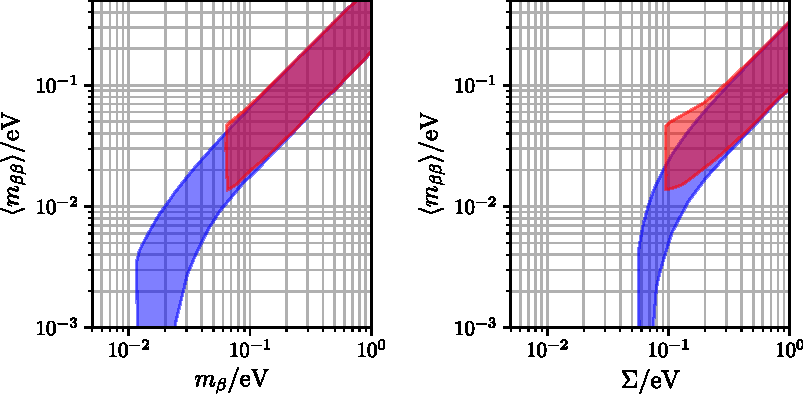
\includegraphics[width=0.8\linewidth]{plots/theory/nu-mass-observables.pdf}
  \caption{%
    The effective mass \mbb\ versus the kinematic neutrino mass observable
    \mb, and the cosmological observable $\Sigma$. The neutrino
    oscillation parameters are varied within their $3\sigma$ ranges. The blue
    (red) area is for the normal (inverted) mass ordering. Taken
    from~\cite{Dolinski2019}.
  }\label{fig:nbb:mass-obs}
\end{figure}

\blocktitle{decay \\ rate}
As we have seen in \cref{eq:nbb:0nudecayrate}, the \onbb\ decay rate can be still
factorized to a good approximation into a phase space factor and a nuclear part, times a
factor encoding the new physics effects generated beyond the Standard Model (the effective
mass in the case of the standard interpretation). Considerations about the theoretical
evaluation of \psft\ and \nmet\ in \cref{sec:nbb:2nbb} are still largely valid for \onbb.
The phase space factor \psfz\ is of the order of $10^{-25}$~yr$^{-1}$ and can be
calculated to a satisfying degree of accuracy~\cite{Kotila2012, Stoica2013} (for \gesix\
it is ${\sim}2.3 \cdot 10^{-15}$~yr$^{-1}$), while nuclear term \nmez\ estimations are in
the 1--10 range but remain terribly affected by large error bars. The situation for the
latter is depicted in \cref{fig:nbb:nme}. As already mentioned in \cref{sec:nbb:2nbb}, the
quenching problem affects also \onbb. Recent studies suggest that there might be less
quenching needed (not more than 20--30\%) in processes with large momentum transfer such
as \onbb~\cite{?}, but there is not yet consensus in the literature. A reduced $g_A$
implies a longer \thalfzero, which is undesirable for experimental searches.  Since no
neutrinos are emitted during the process, the experimental signature of \onbb\ is a
Dirac-delta function at \qbb\ in the summed energy spectrum of the decay products
(\cref{fig:nbb:spectra}).

\begin{figure}
  \centering
  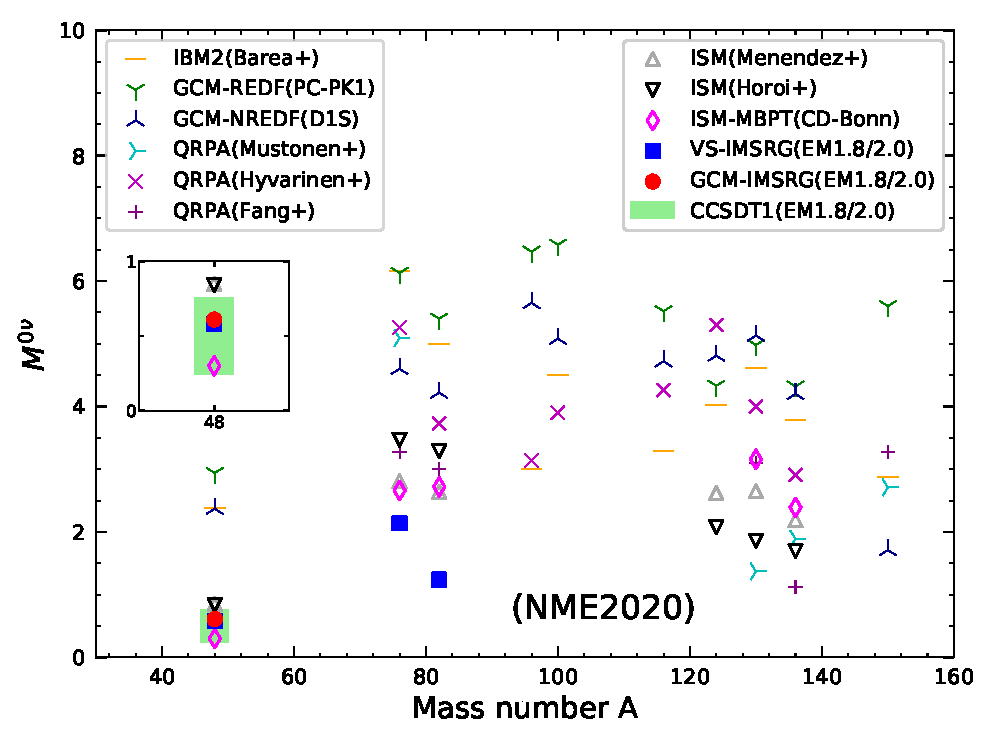
\includegraphics[width=0.6\textwidth]{plots/theory/0nbb-nme.pdf}
  \caption{%
    A representative compilation of nuclear matrix element calculations with an unquenched
    $g_A=1.27$ for different isotopes. Taken from~\cite{Yao2020}. \fillme{replace this
    with plot in \cite{Engel2017}?}
  }\label{fig:nbb:nme}
\end{figure}

\blocktitle{experimental \\ limits}
A compilation of the current most stringent experimental bounds on \thalfzero\ and \mbb\
from \gesix, \nuc{Te}{130} and \nuc{Xe}{136} is given in \cref{tab:nbb:0nbb-lim}. The
\gerda, \kamlandzen\ and CUORE experiments are competing in setting the best half-life
lower limits and \mbb\ upper limits. The experimental program to search for \onbb\ decay
is presented more in detail in \cref{sec:nbb:exp}.

\begin{table}
  \centering
  \caption{%
    Compilation of current most stringent 90\% C.L.~experimental bounds on
    \thalfzero\ and \mbb\ from \gesix, $^{130}$Te and $^{136}$Xe experiments. A
    value of $g_A \simeq 1.27$ is used.
  }\label{tab:nbb:0nbb-lim}
  \begin{tabular}{lcccc}
  \toprule
  Experiment                               & Isotope               & Exposure (\kgyr) & \thalfzero\ (\powtenyr{25}) & \mbb\ (meV)  \\
  \midrule
  \gerda~\cite{Kermaidic2020,Agostini2021} & \mr{2}{\gesix}        & 127.2            & 18                          & 80--102      \\
  \majorana~\cite{Alvis2019}               &                       & 26               & 2.7                         & 200--430     \\
  \midrule
  \cuoricino~\cite{Andreotti2010}          & \mr{3}{\nuc{Te}{130}} & 19.8             & 0.28                        & 300--710     \\
  CUORE-0~\cite{Alfonso2015}               &                       & 9.8              & 0.24                        & 270--760     \\
  CUORE~\cite{Adams2019}                   &                       & 372.5            & 3.2                         & 75--350      \\
  \midrule
  EXO-200~\cite{Anton2019}                 & \mr{2}{\nuc{Xe}{136}} & 234.1            & 3.5                         & 93--286      \\
  \kamlandzen~\cite{Gando2016}             &                       & 594              & 10.7                        & 61--165      \\
  \bottomrule
\end{tabular}

\end{table}

\section{Neutrinoless double-beta decay with Majoron emission}%
\label{sec:nbb:0nbbx}

As mentioned in \cref{sec:nbb:0nbb}, the Majorana nature of the neutrino leads
to the violation of the baryon-lepton number $U{(1)}_{B-L}$ by two units.
Assuming that the symmetry is global and its breaking occurs spontaneously, a
massless Nambu-Goldstone boson, called the Majoron (denoted~$\upchi$), must exist
in the theory~\cite{Chikashige1981, Schechter1982b, Gelmini1981, Georgi1981,
Mohpatra2004}.  Models with massless Majorons have been studied extensively in
the `80 where the Majoron is either a singlet~\cite{Chikashige1981} or part of
a doublet or a triplet~\cite{Gelmini1981, Georgi1981}. However, the last two
possibilities can be ruled out by measurements of the $Z_0$ invisible width at
particle colliders, because of the coupling of the $Z_0$ to the
Majoron~\cite{Berezhiani1992}. All the mentioned models predict neutrinoless
double-beta decay with Majoron emission:
\[
  0\upnu\upbeta\upbeta\upchi:\quad
    \mathcal{N}(A,Z) \longrightarrow \mathcal{N}(A,Z+2) + 2e^- + \upchi
\]
the Feynman diagram is shown in \cref{fig:nbb:majfeydiag}, left. Since the
coupling strength of the singlet `seesaw' Majoron is proportional to $m_{\upnu} /
\Lambda$, where $\Lambda$ is the lepton number breaking energy scale (i.e.~the
heavy right-handed neutrino mass in the seesaw mechanism), obtaining observable
decay rates for \onbbx\ and preserving existing bounds on neutrino masses would
require a severe fine-tuning in the theory~\cite{Burgess1993, Burgess1994}.
\newpar
Another possibility for neutrinoless double-beta decay with Majoron emission
arises in supersymmetric models with R-parity violation~\cite{Masiero1990,
Mohpatra2004}, in which the emission of two Majorons is also
allowed~\cite{Mohpatra1988}:
\[
  0\upnu\upbeta\upbeta\upchi\upchi:\quad
    \mathcal{N}(A,Z) \longrightarrow \mathcal{N}(A,Z+2) + 2e^- + 2\upchi
\]
See \cref{fig:nbb:majfeydiag} (right) for the Feynman diagram of the process.
\newpar
To overcome the fine-tuning problem, many alternative models have been
developed starting from the `90. In this class of models, the term `Majoron'
refers more generically to a light or massless boson, not necessarily a
Goldstone scalar boson, that couples to the neutrino. There are models which
foresee Majorons carrying leptonic charge, thus assuring lepton number
conservation and forbidding \onbb. For the case of Majorons with $L = −2$,
\onbbx\ is expected~\cite{Burgess1993}, while $L = −1$ for the Majoron leads to
\onbbxx~\cite{Burgess1994}. Other models make use of a vector Majoron which
becomes the longitudinal component of a massive gauge boson emitted in
double-beta decay~\cite{Carone1993}, which we will also refer to as `Majoron'
in the latter. A decay process that involves the emission of two Majorons is
also possible~\cite{Bamert1995}.  In~\cite{Mohpatra2000}, the model of a `bulk'
Majoron has been proposed within models featuring extra dimensionalities
(`brane-bulk' scenario for elementary-particle physics).
\newpar
For the sake of completeness, it has to be mentioned that in recent years
models with massive Majorons (\cite{Blum2018} and references therein) have
progressively gained popularity, being this kind of Majoron an appealing dark
matter particle candidate. This hypothesis remains however largely untested
from the experimental point of view, because of the additional level of
complexity added to the double-beta event analysis.

\begin{figure}
  \centering%
  \makebox[\textwidth]{%
    \includegraphics[width=0.5\textwidth]{plots/theory/0nbbxfey.pdf}%
    \includegraphics[width=0.5\textwidth]{plots/theory/0nbbxxfey.pdf}%
  }
  \caption{%
    Feynman graphs for neutrinoless double-beta decay with single (right) and double
    (left) Majoron emission.
  }\label{fig:nbb:majfeydiag}
\end{figure}

\blocktitle{decay \\ rate}
Independently of the model, the decay rate for double-beta decay with Majoron emission can
be factorized as:
\begin{align*}
  \Gamma^{0\upnu\upchi}  &= g_\alpha^2 \cdot G_\alpha^{0\upnu\upchi}(Q_{\upbeta\upbeta}, Z)
    \cdot |M_\alpha^{0\upnu\upchi}|^2 \\
  \Gamma^{0\upnu\upchi\upchi} &= g_\alpha^4 \cdot G_\alpha^{0\upnu\upchi\upchi}(Q_{\upbeta\upbeta}, Z)
    \cdot |M_\alpha^{0\upnu\upchi\upchi}|^2 \;,
\end{align*}
where \ga\ is the effective coupling constant and $\alpha$ denotes the considered
model. The phase space factors can be parametrized as a function of \qbb, the sum kinetic
energy of the two electrons emitted in the decay $K$ and the spectral index $n$:
\[
  G_\alpha^{0\upnu\upchi(\upchi)}(Q_{\upbeta\upbeta}, Z)
    \sim {(Q_{\upbeta\upbeta} - K)}^n \;.
\]
$n = 5$ corresponds to the standard \nnbb\ (i.e.~\cref{eq:nbb:stdmodel}) whereas \onbbx\
can have $n = 1, 2, 3$ and \onbbxx\ can have $n = 3, 7$, depending on the model. As a
consequence, the energy spectrum of the two emitted electrons allows to distinguish the
different models. The energy spectra for all modes of the Majoron emitting double beta
decay are shown in \cref{fig:nbb:majorons-spectra}.

% \begin{table}
%   \centering
%   \caption{%
%     Compilation of up-to-date calculations of phase-space factors
%     \psfmajo~\cite{Kotila2015} and nuclear matrix elements \nmemajo\ for various
%     Majoron-emitting \onbb\ modes and isotopes.
%   }\label{tab:nbb:0nbbx-psf-nme}
%   \begin{tabular}{lcccc}
  \toprule
          & \mc{4}{\psfmajo\ [\powtenyr{-1}] / \nmemajo} \\
  \cmidrule{2-5}
              & $n=1$        & $n=3$        & $n=3$        & $n=7$      \\
  Isotope     & \onbbx\      & \onbbx\      & \onbbxx\     & \onbbxx\   \\
  \midrule
  \gesix\     & \fillme{tbd} & \fillme{tbd} & \fillme{tbd} & \fillme{tbd} \\
  $^{136}$Xe  & \fillme{tbd} & \fillme{tbd} & \fillme{tbd} & \fillme{tbd} \\
  $^{100}$Mo  & \fillme{tbd} & \fillme{tbd} & \fillme{tbd} & \fillme{tbd} \\
  $^{82}$Se   & \fillme{tbd} & \fillme{tbd} & \fillme{tbd} & \fillme{tbd} \\
  $^{116}$Cd  & \fillme{tbd} & \fillme{tbd} & \fillme{tbd} & \fillme{tbd} \\
  $^{48}$Ca   & \fillme{tbd} & \fillme{tbd} & \fillme{tbd} & \fillme{tbd} \\
  $^{150}$Nd  & \fillme{tbd} & \fillme{tbd} & \fillme{tbd} & \fillme{tbd} \\
  $^{130}$Te  & \fillme{tbd} & \fillme{tbd} & \fillme{tbd} & \fillme{tbd} \\
  $^{96}$Zr   & \fillme{tbd} & \fillme{tbd} & \fillme{tbd} & \fillme{tbd} \\
  \bottomrule
\end{tabular}

% \end{table}

\begin{figure}
  \centering
  \includegraphics{plots/theory/majorons-spectra.pdf}
  \caption{%
    Two-electron energy spectra from different models (labeled by the spectral index $n$,
    see text) of double-beta decay of \gesix, including the standard \nnbb, the
    Lorentz-violating mode \nnbblv\ and the Majoron emitting modes.  Analytic formulas,
    obtained with the Primakoff-Rosen approximation, for the Fermi function are taken
    from~\cite{Tretyak1995, Tretyak2002}.
  }\label{fig:nbb:majorons-spectra}
\end{figure}

\blocktitle{experimental \\ limits}
A compilation of the most recent experimental 90\% C.L.~lower limits on the half-life of
Majoron-emitting \onbb-decay for several nuclei is given in \cref{tab:nbb:0nbbx-lim}. To
compare the experimental sensitivity, the upper limit on \ga\ is calculated for the spectral
index $n=1$, for which the half-life limit is usually higher. Phase space factors
\psfmajo\ are taken from~\cite{Kotila2015}, nuclear matrix elements \nmemajo\
from~\cite{Engel2017}. The most stringent limits at the moment are for \nuc{Xe}{136} from
EXO-200 and \kamlandzen.

\begin{table}
  \centering
  \caption{%
    A compilation of the current 90\% C.L.~lower limits on Majoron-emitting \onbb\ modes
    as set by the \gerda, EXO-200, KamLAND-Zen and NEMO-3 experiments for different
    isotopes. The limit on the coupling constant \ga\ for $n=1$ is reported, as calculated
    with phase-space factors from~\cite{Kotila2015} and most up-to-date nuclear matrix
    elements~\cite{Engel2017}. \ga\ limits for the other indices and different models can
    be found in the references.
  }\label{tab:nbb:0nbbx-lim}
  \begin{tabular}{lcccccccc}
  \toprule
                                      &               &                  & \mc{4}{\thalfmajo\ (\powtenyr{21})} &             \\
  \cmidrule{4-7}
  Experiment                          & Isotope       & Exposure (\kgyr) & $n=1$ & $n=2$ & $n=3$ & $n=7$       & $g_\alpha$  \\
  \midrule
  \gerda~\cite{Agostini2015a}         & \gesix\       & 20.3             & 420   & 180   & 80    & 30          & \fillme{tbd}\\
  EXO-200~\cite{Albert2014a}          & \nuc{Xe}{136} & 100              & 1200  & 250   & 27    & 6.1         & \fillme{tbd}\\
  \kamlandzen~\cite{Gando2012}        & \nuc{Xe}{136} & 36.8             & 2600  & 1000  & 250   & 11          & \fillme{tbd}\\
  NEMO-3~\cite{Arnold2013,Arnold2019} & \nuc{Mo}{100} & 34.3             & 44    & 9.9   & 4.4   & 1.2         & \fillme{tbd}\\
  NEMO-3~\cite{Arnold2018}            & \nuc{Se}{82}  & 4.9              & 37    & --    & --    & --          & \fillme{tbd}\\
  NEMO-3~\cite{Arnold2016}            & \nuc{Cd}{116} & 2.16             & 8.5   & --    & --    & --          & \fillme{tbd}\\
  NEMO-3~\cite{Arnold2016a}           & \nuc{Ca}{48}  & 0.037            & 4.6   & --    & --    & --          & \fillme{tbd}\\
  NEMO-3~\cite{Arnold2016b}           & \nuc{Nd}{150} & 0.19             & 30    & --    & --    & --          & \fillme{tbd}\\
  NEMO-3~\cite{Arnold2011}            & \nuc{Te}{130} & 2.31             & 16    & --    & --    & --          & \fillme{tbd}\\
  NEMO-3~\cite{Argyriades2009}        & \nuc{Zr}{96}  & 0.031            & 1.9   & 0.99  & 0.58  & 0.11        & \fillme{tbd}\\
  \bottomrule
\end{tabular}

\end{table}

\section{Lorentz-violating two-neutrino double-beta decay}%
\label{sec:nbb:2nbbLV}

Since the Standard Model of Particle Physics is known to provide a successful description
of most physics at low energies, compared to the Planck scale $m_p {\sim}10^{19}$~GeV, any
signal of new physics must appear at low energies in the form of an effective quantum
field theory containing the Standard Model.  The general effective quantum field theory
constructed from the latter and allowing for arbitrary coordinate-independent Lorentz
violation is called the Standard Model Extension~\cite{Colladay1997, Colladay1998}. As an
effective field theory it provides a link to the Planck scale through operators of
non-renormalizable dimension. The Lagrangian of the Standard Model Extension consists of
the usual Standard Model Lagrangian supplemented by all possible terms that can be
constructed with the existing fields and that introduce violations of Lorentz symmetry.
The additional terms have the form of Lorentz-violating operators coupled to vector
coefficients, and they could arise in a variety of ways.
\newpar
All quantum field operators for Lorentz violation involved in the propagation of neutrinos
have been classified and enumerated~\cite{Kostelecky2012}. Most of these can be studied
using neutrino oscillations, which compare the way different neutrinos propagate and
provide interferometric sensitivity to energy differences between
them~\cite{Kostelecky2003, Diaz2014}. Some effects cannot be detected by neutrino
oscillations because they are produced by `oscillation-free' operators that change all
neutrino energies equally. Most of these can instead be studied by comparing neutrino
propagation to other species, such as time-of-flight experiments that match the group
velocity of neutrinos and photons~\cite{Adam2011}.  However, four oscillation-free
operators leave unaffected the neutrino group velocity and cannot be detected in this way.
Instead, they must be accessed through physical processes that involve neutrino
phase-space properties, such as particle decays. These operators are rare examples of
\textit{countershaded} Lorentz violations~\cite{Kostelecky2009}: Relativity-violating
effects that could be enormous compared to ones suppressed by the ratio $m_W/m_P$ and that
nonetheless could have escaped detection to date. These could provide an interesting path
for building models with viable Lorentz violation obviating the typical requirement of a
heavy suppression factor.
\newpar
The four countershaded neutrino operators are of renormalizable mass dimension $d=3$, are
odd under \cpt, and are controlled by coefficients conventionally denoted with
$(a^{(3)}_\text{of})_{jm}$, where $j$ and $m$ are angular-momentum quantum numbers with $j
= 0,1$. Non-zero values of \aofoo\ could produce small deviations in the shape of the
energy spectra of electrons emitted in \b\ and double-\b\ decays~\cite{Diaz2013a}.
Conservation of energy and momentum is assured by taking these four coefficients to be
constant as usual for couplings beyond the Standard Model, so all physics other than
Lorentz and \cpt\ violation is conventional. Dimensional arguments suggest these
coefficients are likely to dominate at accessible energies and can be measured sensitively
in low-energy processes.
\newpar
The anti-neutrino phase space element $\text{d}^3q$ is modified by the presence
of these new operators:
\[
  \omega^2\text{d}\omega\text{d}\Omega \;\longmapsto\;
    f(\omega)\text{d}\omega\text{d}\Omega\;,
\]
where the anti-neutrino function
\(f(\omega)\simeq\omega^2-\frac{1}{2}m_\nu^2-2\omega\delta\omega\)
encodes the Lorentz-violating modifications
\[
  \delta\omega = -\sum_{jm} e^{im\omega_\oplus T_\oplus}
  \mathcal{N}_{jm}{(a_\text{of}^{(3)})}_{jm}
\]
arising from the modified anti-neutrino dispersion relation~\cite{Kostelecky2012} $\omega
= |\vec{q}| + m_\nu^2 / |\vec{q}| + \delta\omega$. The sidereal time $T_\oplus$
controls the harmonic variation of the anti-neutrino function in the laboratory produced
by the Earth sidereal rotation at frequency $\omega_\oplus \simeq
2\pi/(23\text{h}~56\text{min})$.  The factors $\mathcal{N}_{jm}$ contain information about
the direction of propagation of the anti-neutrinos, expressed relative to the canonical
sun-centered frame of reference~\cite{Bluhm2003, Kostelecky2002}.

\blocktitle{decay \\ rate}
Following the same procedure and adopting the necessary approximations as in the
conventional two-neutrino double-beta decay (\cref{sec:nbb:2nbb}), one can integrate over
all orientation, which implies that only isotropic effects are observable and hence that
the residual spectrum depends only on $\aofM \equiv \aofooM/\sqrt{4\pi}$. After a suitable
change of integration variables and defining the sum of kinetic energies $K=T_1+T_2$ for
the two electrons, the electron sum spectrum reads
\begin{equation}\label{eq:nbb:totwidth}
  \begin{split}
    \frac{\text{d}\Gamma}{\text{d}K} = &
      \Lambda \cdot (K^5 + 10K^4 + 40K^3 + 60K^2 + 30K) \\
      & \times\left[{(Q_{\beta\beta} - K)}^5 + 10 \aofM {(Q_{\upbeta\upbeta} - K)}^4\right] \;. \\
  \end{split}
\end{equation}
The total decay rate can be therefore expressed as an addition of two separate
rates through a perturbation:
\[
  \Gamma = \Gamma_0 + \delta\Gamma = g_A^4 |m_e c^2 \mathcal{M}^{2\upnu}|^2 (G^{2\upnu} +
  \delta G^{2\upnu}) \;,
\]
where the first term is \cref{eq:nbb:stdmodel} and the second one is the perturbation
introduced by Lorentz violation. Detailed calculations can be found
e.g.~in~\cite{Nitescu2020}. The summed-electron energy spectrum generated by the
perturbative term is depicted in \cref{fig:nbb:majorons-spectra}. The proportionality
between the decay rate represented by $\Gamma_0$ (i.e.~the standard \nnbb\ decay
amplitude) and the decay rate relative to the perturbation $\delta\Gamma$ is set by the
\aof\ coefficient:
\[
  \frac{\delta\Gamma}{\Gamma_0} = 10 \aofM \mathcal{R} \;.
\]
Values for the $\mathcal{R}=\aofM G^{2\upnu} / \delta G^{2\upnu}$ coefficient have been
computed in~\cite{Nitescu2020} using radial solutions of the Dirac equation to express the
Fermi function $F(Z,E)$.

\blocktitle{experimental \\ limits}
Conservative constraints on $|(a_\text{of}^{(3)})_{j0}|$ coefficients have
been placed using published results from the Troitsk and Mainz experiments
studying the endpoint of the tritium beta decay energy
spectrum~\cite{Diaz2013}. An outside analysis of data from the two experiments
gives $|(a_\text{of}^{(3)})_{j0}| < 2 \cdot 10^{-8}$~GeV for both $j=0,1$.
Constraints on the values of \aof\ have also been extracted from studies of
threshold effects in pion and kaon decays~\cite{Kostelecky2012}, yielding
$\aofM < 1.9 \cdot 10^{-7}$~GeV as the best upper limit.  Since many
double-beta experiments have now accumulated high-statistic \nnbb\ datasets,
constraints on \aof\ has been recently posed with \nuc{Te}{130}, \nuc{Xe}{136} and
\nuc{Mo}{100}. Published limits are summarized in \cref{tab:nbb:2nbblv-lim}.

\begin{table}
  \centering
  \caption{%
    Compilation of current experimental bounds at 90\% C.L.~on the Lorentz-violating \aof\
    coefficient from double-beta decay.
  }\label{tab:nbb:2nbblv-lim}
  \begin{tabular}{lccc}
  \toprule
  Experiment                  & Isotope    & Exposure (\kgyr) & \aof\ (GeV) \\
  \midrule
  CUPID-0~\cite{Azzolini2019} & $^{130}$Te & 9.95             & $< 4.1 \cdot 10^{-6}$           \\
  EXO-200~\cite{Albert2016}   & $^{136}$Xe & 100              & $\in [-2.65, 76] \cdot 10^{-5}$ \\
  NEMO-3~\cite{Arnold2019}    & $^{100}$Mo & 34.3             & $\in [-4.2, 3.5] \cdot 10^{-7}$ \\
  \bottomrule
\end{tabular}

\end{table}

\section{From theory to the experimental practice}%
\label{sec:nbb:exp}

The primary focus of experiments that involve double-beta decay is the search for the
neutrinoless decay mode, by far the most important compared to other processes. The
observables in direct searches of \onbb\ are the kinematic parameters of the two emitted
electrons. A typical experiment measures the total energy of the two electrons (the only
observable that is both necessary and sufficient for discovery) and may have the
capability to reconstruct the electron tracks in order to reject background events with
different event topologies. Since \qbb\ is usually known to a high degree of accuracy and
the \onbb\ signature is a mono-energetic peak at \qbb, the signal search is performed in a
narrow energy window defined by the energy resolution of the detector.

\blocktitle{background \\ level}
The number of signal counts in this Region Of Interest (ROI) depends linearly on the
detector signal efficiency $\epsilon$, the active mass $M$, the measurement time $t$ and
the isotopic fraction of the double-beta emitter $a$.  These are the quantities that
usually play a fundamental role when designing an experiment. The sensitivity to the
half-life \thalfzero\ scales linearly with the number of candidate signal counts in the
ROI, but the dependence is weaker if some of them are background counts. Two experimental
regimes can be defined:
\begin{equation}\label{eq:nbb:bkglevel}
  T^{0\upnu}_{1/2} =
    \begin{cases}
      a M \epsilon t & \text{background-free} \\
      a \epsilon \sqrt{\frac{M t}{B \Delta{E}}} & \text{with background} \;, \\
    \end{cases}
\end{equation}
where $B$ is the `background index', namely the number of background events normalized to
the width of the ROI, source mass and measurement time. This expression clearly shows the
advantage of a background-free experiment, since the \thalfzero\ scales linearly with $t$
as opposed to $\sqrt{t}$ in the presence of backgrounds. The background-free condition is
effectively realized when the expected number of background events in the ROI in the
measurement time $t$ is of the order of unity:
\[
  M \cdot T \cdot B \cdot \Delta{E} \lesssim 1 \;.
\]

\blocktitle{isotope \\ choice}
Not all the double-beta emitters that exist in Nature can be effectively employed to
search for \onbb. As it can be clearly understood from \cref{eq:nbb:bkglevel}, an ideal
isotope should have a high isotopic abundance $a$, should be available in large quantities
$M$ as high-resolution $\Delta{E}$ detectors under low background conditions $B$. Other
relevant isotope features are a low \nnbb\ decay rate to mitigate the occurrence of
background events in the ROI, and a high \qbb\ to avoid backgrounds from primordial
radioisotopes which are naturally present in construction materials. Moreover, the
detection efficiency $\epsilon$ can be drastically enhanced if the source material is
integrated in the detector medium.  A good double-beta emitter should also be readily
available in its natural form and have a high natural abundance, to reduce the cost of the
experiment. If natural abundance is high enough, isotope enrichment might also be
unnecessary, as demonstrated in the case of $^{130}$Te~\cite{Alduino2017}.

\blocktitle{backgrounds}
To achieve the ambitious goal of operating in a background-free regime, the
next-generation experiments need to fight against many different background sources. Here
a short summary of the main experimental issues concerning this topic is given. The only
irreducible background to \onbb\ signal searches is given by \nnbb\ events. A careful
isotope and detector technology choice can mitigate the impact of such a contribution,
since the number of \nnbb\ events that can leak in the ROI reduces with increasing energy
resolution.  Solar neutrino interactions are also expected to be relevant in tonne-scale
detectors, and the respective background contribution can be mitigated by a high mass
loading of the decaying isotope in the target medium. As already mentioned, radioisotopes
from the uranium and thorium decay chains are ubiquitous in construction materials and
their presence must be kept to a minimum. Material radio-purity must be kept high during
production and later on before installation, to avoid, among the others, contamination by
exposure to \Rn. Natural radioactivity from components far away from the active source,
e.g.~rock walls of an underground laboratory, can be passively screened with clean lead or
copper, water or cryogenic liquid. The latter two options allow the shielding medium to
serve also as an active shield vetoing background events. Cosmic rays can also induce
several type of backgrounds. Prompt muon interactions typically deposit large amount of
energy in detectors and can be easily vetoed. Backgrounds coming from secondary neutrons
and cosmogenically-activated isotopes are the main worries. The latter can be avoided by
minimizing the exposure of the active material to cosmic rays on the Earth's surface and
rapidly deploying them underground.

\blocktitle{experimental \\ approaches}
Neutrinoless double-beta decay has a characteristic event topology with the emission of
two $\sim$MeV electrons. Low-density-gas tracking detectors can in principle resolve the
two electron tracks, leaving only the irreducible background from \nnbb\ decay. For
detectors with higher density, such as discrete detectors or liquid scintillator
detectors, these electrons deposit their energy within a few millimeters, allowing a less
powerful but still useful discrimination between `compact' signal-like events and \g\
rays, which are likely to scatter and deposit energy at multiple sites. The difference may
be resolved through discriminating between the `single-site' and `multi-site' events by
pulse-shape discrimination or reconstructed event topology, depending on the position
resolution, as well as the size and type of a given detector.  Some detectors are capable
of particle discrimination through multiple detection channels, e.g.~scintillation and
ionization. This could allow for the identification of \a\ backgrounds. Other
discrimination techniques exploit the spatial distribution of background events, if
consistently different from that of the signal events. If background events coming from
mechanical support materials are concentrated close around them they might be rejected by
an optimized fiducial volume cut, if a monolithic detector is used. In presence of a
discrete detector, instead, multi-detector event cuts can be used to isolate double-beta
point-like events.

\begin{description}[wide]

  \item[Semiconductors] One of the most promising approaches for scaling to tonne-scale
    experiments is using \gesix-enriched High-Purity Germanium (HPGe) detectors, which
    serve as active source and target for \onbb\ at the same time. The main advantages of
    using HPGe detectors are the maturity of the industrial production technologies, their
    intrinsic purity and the superior energy resolution (per-mill level at \qbb).  A clear
    disadvantage of these detectors is their production cost and the low \qbb\ of
    $\sim$2~MeV. The current generation of \gesix\ experiments is constituted by
    \gerda~\cite{Budjas2013} and \majoranademo~\cite{Abgrall2014}, whose collaborations
    are currently joining their efforts into the next-generation LEGEND experimental
    program~\cite{Abgrall2017}. Its first phase, LEGEND-200, is expected to start data
    taking in 2021 while its planned tonne-scale phase LEGEND-1000, aims at $\thalfzeroM
    {\sim}10^{28}$~yr sensitivity.

  \item[Bolometers] Bolometers are cryogenic calorimeters that operate at temperatures of
    $\sim$10~mK. An absorber is connected to the thermal bath via a weak thermal link, and
    the temperature is read out by a sensitive thermometer. Crystal absorbers can be grown
    from many materials that include double-beta decay isotopes, e.g.~TeO$_2$,
    $^{116}$CdWO$_4$, Zn$^{82}$Se, $^{40}$Ca$^{100}$MoO$_4$, Zn$^{100}$MoO$_4$ and
    Li$_2^{100}$MoO$_4$.  Advantages of this detector technology are the intrinsically low
    crystal radioactivity and the high energy resolution. The challenge is to operate a
    large-scale detector at these ultra-low temperatures. Existing projects that exploit
    the bolometric technique are CUORE~\cite{Arnaboldi2002, Artusa2014}, that takes
    advantage of the large natural abundance of \nuc{Te}{130}, CUPID~\cite{Wang2015}, which
    explores the possibility to improve the background rejection in CUORE through active
    particle discrimination, and \textsc{AMoRE}, a \nuc{Mo}{100}-based
    experiment~\cite{Kim2015}. The ultimate sensitivity goal of the CUPID and
    \textsc{AMoRE} tonne-scale program is $\thalfzeroM > 10^{27}$~yr and $\thalfzeroM
    \sim 5 \cdot 10^{26}$~yr, respectively.

  \item[Time Projection Chambers] The time projection chamber (TPC) is an attractive
    detector technology for \onbb-decay searches because of a combination of mass
    scalability and access to multiple background discrimination variables. A TPC takes
    advantage of a detection medium that produces two energy channels: ionization and
    scintillation. The combination of these two signals allows the reconstruction of event
    topology, position, energy and particle type. \nuc{Xe}{136} is a convenient source and
    detector medium for both liquid- and gas-phase TPCs. By operating high-pressure
    gas-phase xenon TPCs in electroluminescent mode, an energy resolution of better than
    0.5\% FWHM at \qbb\ can be achieved. Liquid-phase xenon TPCs, instead, offer maximum
    source density. Since \onbb\ searches focus on low background and good energy
    resolution, single-phase detectors are usually chosen for liquid-phase TPCs. The
    achievable energy resolution is somewhat worse than that of the gas-phase detectors,
    but multi-site background and spatial distribution discrimination work well with
    position resolution achievable at the few-mm level. Notable projects focusing on the
    liquid-xenon single-phase TPC technology to search for \onbb\ are
    EXO-200~\cite{Auger2012} and its proposed tonne-scale successor,
    \textsc{nEXO}~\cite{Kharusi2018}, which aims at $\thalfzeroM {\sim}10^{28}$~yr
    sensitivity.  Planned high-pressure xenon gas-phase TPC projects are
    NEXT~\cite{Lopez-March2017} (\thalfzero\ sensitivity goal $2.8 \cdot 10^{25}$~yr with
    NEXT-100) and \textsc{PandaX-III}~\cite{Chen2016} (\powtenyr{27} sensitivity goal
    within its tonne-scale program). Two-phase liquid-xenon detectors, popular for dark
    matter searches, such as LUX-ZEPLIN~\cite{Akerib2015},
    \textsc{XENON-nT}~\cite{Aprile2017} and the future DARWIN~\cite{Aalbers2016} might
    also have the capability to search for \onbb\ decay.

  \item[Scintillators] The main appeal of organic scintillators for \onbb\ searches is
    their mass scalability, despite their poor energy resolution.  Another advantage of
    liquid target masses is the possibility to remove contaminants online. A notable
    experiment exploiting this detection approach is \kamlandzen, which loaded nearly
    400~kg of enriched xenon (\kamlandzen\ 400, Phase~II). The collaboration is currently
    starting the new KamLAND-Zen 800 phase, that will load 750~kg of enriched xenon. In
    the longer term, the KamLAND-Zen collaboration plans to deploy over a tonne of
    enriched xenon and to reduce the \nnbb-decay background in the signal region of
    interest by improving the detector resolution in the \textsc{KamLAND2-Zen} experiment and
    reaching a \thalfzero\ sensitivity of ${\sim}2 \cdot 10^{27}$~yr. Searching \onbb\
    decay with $^{130}$Te is the main goal of another liquid scintillator experiment,
    SNO+~\cite{Andringa2015}, which is currently loading its target medium with the source
    isotope~\cite{Paton2019}. Also inorganic CaF$_2$ scintillators have been always
    receiving interest, because of the high $^{48}$Ca \qbb\ of 4.27~MeV. However, finding
    a cost effective process to enrich the isotope, whose natural abundance is only
    $\sim$0.2\%, is still a challenge. The CANDLES series~\cite{Umehara2015} of \onbb\
    searches at the Kamioka Observatory is actively exploring this experimental approach.

  \item[Tracking Calorimeters] The \textsc{SuperNEMO}~\cite{Arnold2010} unique
    experimental programs, based on the technology demonstrated by
    NEMO-3~\cite{Arnold2004}, uses a thin foil of source material in the center of a
    sandwich configuration, surrounded first by a low-pressure gas tracking layer to track
    the two \b\ particles and then a calorimetric layer to measure the energy. This type
    of detectors provides superior topological information and is the only detector
    technology capable of measuring the opening angle between the two {\b}s --- one
    observable that can distinguish certain underlying mechanisms for \onbb\ decay. In
    addition, many different isotopes can be formed into foils and studied in the same
    detector configuration. The advantage of this detection approach is the excellent
    background discrimination, which allows to easily reach a zero-background condition.
    However, the low energy resolution does not permit to efficiently discriminate between
    \nnbb\ and \onbb\ events around \qbb, plus the detection efficiency is low (around
    30\%) and the thin source foils are difficult to scale up to large exposures. The
    sensitivity with $^{82}$Se for a full \textsc{SuperNEMO} is projected to be $1.2 \cdot
    10^{26}$~yr.

\end{description}

\chapsummary
\begin{itemize}
  \item Double-beta decay is a rare nuclear decay process in which two electrons and two
    electron anti-neutrinos are emitted. The decay rate can be factorized in a phase space
    factor, that can be calculated to a high degree of accuracy, and a nuclear matrix
    element, which is notoriously much more difficult to evaluate. Several numerical
    approaches to the problem have been proposed, which give inconsistent results. The
    energy spectrum of the two emitted electrons is a continuous distribution between zero
    and the Q-value of the reaction.
  \item Neutrinoless double-beta decay is an hypothetical decay mode in which no neutrinos
    are present in the final state. The occurrence of such a process is connected to the
    fundamental properties of the neutrino and the origin of the our matter-dominated
    universe. The observation of neutrinoless double-beta decay would establish the
    Majorana nature of the neutrino and imply the existence of physics beyond the Standard
    Model. The observable connected to the neutrino mass tested by neutrinoless
    double-beta decay is the so-called `effective Majorana mass'. The experimental
    signature of the decay is a mono-energetic peak in the summed energy spectrum at the
    Q-value. No experiments have conclusively collected evidence of the existence of the
    decay so far.
  \item Since neutrinoless double-beta decay requires a symmetry breaking in the model, a
    massless bosonic particle, the so-called Majoron, must exist in the theory. Many
    theories predict the presence of Majorons in the final state of the decay process.
    Another hypothetical process is the Lorentz and CPT violating two-neutrino double-beta
    decay, which has been proposed in the framework of the Standard Model Extension. The
    experimental signature of these exotic decay modes is a distortion of the standard
    two-neutrino double-beta decay spectrum, regulated by the coupling constant \ga\ in
    presence of Majorons or the \aof\ coefficient in the case of Lorentz symmetry
    violation.
  \item Several experimental aspects are of fundamental importance when searching for
    neutrinoless double-beta decay in laboratories. The so-called background-free
    condition, in which the sensitivity to the signal scales linearly with exposure time,
    is realized when the expected number of background events at the double-beta decay
    Q-value is of the order of unity. The current and planned experimental program is rich
    and vast. Science collaborations that deploy semiconductors, bolometers, time projection
    chambers, scintillators and tracking calorimeters are challenging each other in
    setting the most stringent limit on the neutrinoless double-beta decay half life, if
    not finding a signal.
\end{itemize}

% vim: tw=90

  %!TEX root = ../main.tex

\chapter{The \gerda\ experiment}\label{chap:gerda}

The GERmanium Detector Array (\gerda) experiment has been proposed in
2004~\cite{gerda-proposal} to search for neutrinoless double-beta decay with High-Purity
Germanium detectors (HPGe) enriched in the \gesix\ double-beta emitter. The proposal lies
in the path opened by the Heidelberg-Moscow (\hdm)~\cite{Klapdor2001} and
\igex~\cite{Aalseth2002} experiments, aiming to develop the germanium technology towards
large-scale, background-free experimental conditions that could tackle the scale of
$\mathcal{O}(10^{26})$~yr sensitivity on the neutrinoless double-beta decay half-life. The
history of the achievements in \thalfzero\ limit setting and background level with \gesix\
is presented in \cref{img:exp:ge76-history}, top. On the bottom plot, a zoom in the
\gerda\ data taking period showing the experimental progresses in terms of \thalfzero\
sensitivity, lower limit and collected active exposure.  \gerda\ data taking officially
ended in December 2019 after hitting the target total background-free exposure of 100~\kgyr\ and
establishing itself as the leading experiment in the field in terms of lowest background
level ever achieved around \qbb~\cite{Agostini2019a}.

\blocktitle{\gerda\ \\ phases}
Since the start of the data taking in 2008 the experiment, located in hall~A of the Gran
Sasso National Laboratories (LNGS) in Italy, has been running through two distinct
experimental phases (\phaseone\ and \phasetwo). Detectors from the former \hdm\ and \igex\
experiments (of semi-coaxial geometry) along with newly produced diodes (of \bege\
geometry type, shorthand for Broad Energy Germanium detectors) were deployed bare into
liquid argon (LAr) during \phaseone, following a suggestion by ref.~\cite{Heusser1995},
for a total amount of 21.3~kg of germanium. \phaseone\ ended in June 2013 with a total
exposure of 21.6~\kgyr\ and a background index in the region of interest of
\pIbi~\cite{Agostini2016}.  Shortly after that the upgrade works for \gerda\ \phasetwo\ started:
a new event veto system based on the LAr scintillation light was installed along with an
additional 20~kg of \bege-type detectors.  The newly designed veto system set the stage for a
significant reduction of the background index (BI) down to the \powctsper{-4} scale, allowing
\gerda\ to seamlessly run in background-free conditions for its full second experimental phase
and surpass the \powtenyr{26} sensitivity threshold in April 2018~\cite{Agostini2019a}.
Data taking was then stopped again to permit a third hardware upgrade, during which
another 9.6~kg of enriched germanium in the form of five inverted-coaxial geometry
detectors was deployed\footnote{Note however that a semi-coaxial detector (\ANG{1}) and
the natural \GTF{} detectors were removed.}. Moreover, the LAr veto system was exchanged
with a more efficient one, thanks to the denser fiber curtain and the addition of a shroud
enclosing the central string, now consisting of inverted-coaxial detectors only. This last
part of \phasetwo, which will be referred as \phasetwop\ in the following, ended in
December 2019 after collecting the total exposure of \fillme{fillme}~\kgyr\ and
establishing the final \gerda\ upper limit on the neutrinoless double-beta decay half-life
of \gerdafinallimit. When generally referring to the \phasetwo\ period, if not specified
in the following, \phasetwop\ must be considered as implicitly included.
\begin{figure}
  \centering
  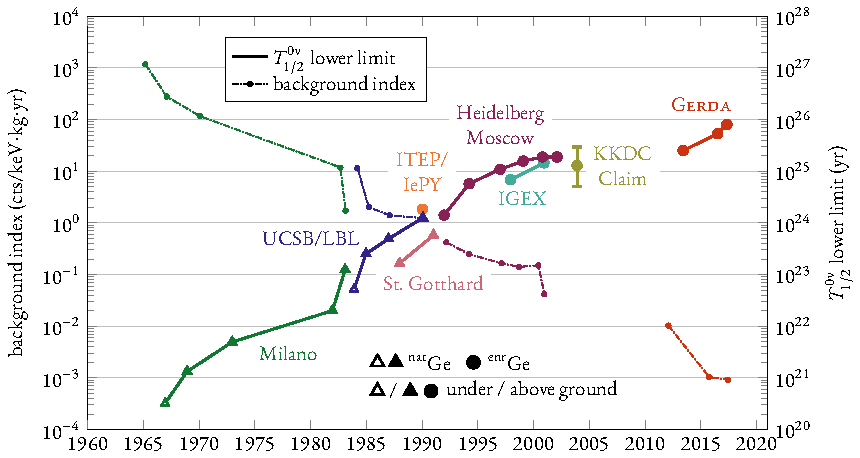
\includegraphics{plots/0nbb-ge76-history.pdf}
  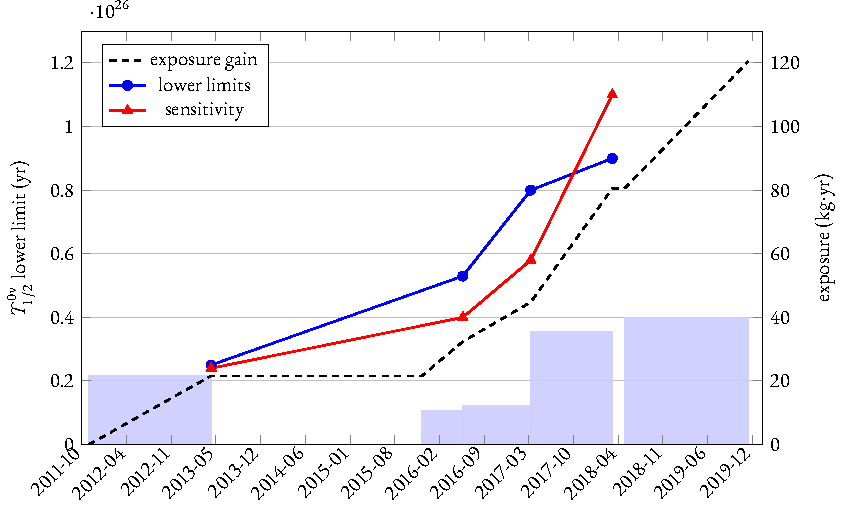
\includegraphics{plots/gerda-history.pdf}
  \caption{%
    Top: history of lower limits (68\% CL, 90\% CL since 1991) and background indices from
    \gesix\ neutrinoless double-beta decay experiments, extracted from~\cite{Fiorini1967,
    Bellotti1984, Caldwell1989, Reusser1991, Vasenko1989, Klapdor2001, Aalseth2002,
    Klapdor2004, Alvis2019, gerda-final} and references therein. Original design by Karl-Tasso
    Kn\"opfle.  Numbers attached to single data points correspond to exposures in
    mol(\gesix)$\cdot$yr. Bottom: evolution and milestones set by the \gerda\ experiment
    through its three experimental phases. The exposure gain, the neutrinoless double-beta
    decay half-life sensitivities and upper limits are tracked over time. \fillme{to be
    updated}
  }\label{img:exp:ge76-history}
\end{figure}
\newpar
The \phasetwop\ upgrade is partly also a test bench for the next-generation successor of
\gerda\ in the field of double-beta decay physics with \gesix, the LEGEND experiment. The
collaboration, formed in October 2016 from the \gerda\ and \majorana~\cite{Abgrall2014}
(the latter experiment is searching for \onbb\ with germanium detectors at the Sanford
Underground Research Facility (SURF) in USA), pursues the goal of building a tonne-scale
\gesix\ experiment and reaching the $\mathcal{O}(10^{28})$~yr sensitivity scale. The first
phase of the experiment, LEGEND-200, will deploy 200~kg of germanium in the existing \gerda\
infrastructure at LNGS and it is currently in commissioning phase.
\newpar
As the present thesis work focuses on \gerda\ \phasetwo\ data, the description of the
experimental setup and the main analysis techniques given in the following will be limited
to that time period. The chapter is structured as follows. In \cref{sec:gerda:setup} a
general overview of the \gerda\ \phasetwo\ (and \phasetwop) apparatus is given. In
\cref{sec:gerda:cuts} the working principles of the main background reduction techniques
that allow \gerda\ to operate in the background-free regime are outlined. The application
of these event-selection criteria to the \phasetwo\ data, the statistical analysis of the
events at \qbb\ and the final results are presented in \cref{sec:gerda:ana}.

\section{Overview of the Phase {\normalfont\textit{II}} experimental setup}%
\label{sec:gerda:setup}

The \gerda\ experiment is located in hall~A of the LNGS laboratories, at a depth of about
3500~m water equivalent, to suppress cosmogenically-induced background
sources~\cite{Wiesinger2018}. The germanium detectors are arranged into strings within a
cryostat filled with 64~m$^3$ of liquid argon (LAr), which acts as a shielding and cooling
medium at the same time. The cryostat itself is enclosed by a large tank containing
590~m$^3$ of ultra-pure water.  Besides the additional shielding effect, this water layer
act as a medium for a \v{C}erenkov veto system with 66 photomultiplier tubes (PMTs)
against muons. An array of scintillating panels is installed on the top of the clean room
to complete the muon veto system~\cite{Freund2016} (see \cref{fig:setup:pictures}a). A
simplified representation of the experimental setup is given in \cref{fig:setup:overview},
together with a picture taken from the outside.

\begin{figure}
  \centering
  \includegraphics[width=\textwidth]{setup/gerda-overview.pdf}
  \caption{%
    On the right: artist view of the \gerda\ experimental setup. On the left: a picture of
    taken during the inauguration in November 2010. The experiment, installed in hall A of
    the Gran Sasso National Laboratories in Italy, deploys an array of germanium detectors
    enriched in \gesix\ bare in liquid argon, together with a liquid argon scintillation
    light veto system. The cryostat is submerged in a water tank to provide additional
    shielding from external background sources. A plastic scintillating panel system is
    installed on the top of the whole structure as an active muon veto, together with the
    water tank.
  }\label{fig:setup:overview}
\end{figure}

\blocktitle{detectors}
The \gerda\ \phasetwo\ array is organized in 7 vertical strings, holding 40 detectors in
total. The detectors can be divided in three groups: the \bege\ detectors, the
semi-coaxial \m{ANG} and \m{RG}, and the semi-coaxial \m{GTF} detectors. The detectors of
the first two groups are made of germanium enriched in \gesix, the third group includes
detectors with natural isotopic germanium abundance. During the upgrade works for
\phasetwop\ in 2018 four enriched inverted-coaxial \IC{} detectors were introduced to
replace the three \GTF{} detectors in the central string, for a total of 41 detectors
deployed.
\newpar
All \gerda\ HPGe detectors are made of high-purity p-type germanium, which is initially
used to pull crystals, typically fuse-shaped (see for example fig.~4.1a in
\cite{Yonenaga2019}).  Crystals are then cut in slices, and each of them is further
processed to obtain the final detector geometry. The electrodes for signal read-out and
voltage biasing are then fabricated on the detector surface. The \nplus\ contact, where the
external voltage is applied, `wraps around' the detector. It is obtained by deposition of
a lithium layer on the surface, which diffuses below the surface until a depth of
$\sim$1~mm during the subsequent thermal annealing cycles. The presence of lithium
impurities effectively creates a region with decreased charge collection efficiency (CCE),
or `dead-layer', even when biased at full-depletion voltages.  In this region, the CCE is
zero at the surface and reaches its maximal value at the full charge collection depth
(FCCD). The \pplus\ electrode, where the signal is read out, is instead fabricated by boron
implantation, and the dead layer it produces is typically smaller, at the level of
hundreds of microns. The two conductive surfaces are separated by an insulating region,
which is typically produced by excavating a `groove'. In some cases such groove is
passivated by deposition of a germanium-oxide layer.
\newpar
\blocktitle{%
  \includegraphics[width=15mm]{gedet/BEGe.png}\\
  \includegraphics[width=15mm]{gedet/SemiCoax.png}\\
  \vspace{2mm} % tweak
  \includegraphics[width=15mm]{gedet/InvCoax.png}%
}
The \gerda\ \phasetwo\ detectors before the 2018 upgrade can be classified according to
two different geometry types: semi-coaxial and \bege. In the semi-coaxial design, a
bore-hole is excavated along the central axis to accomodate the \pplus\ electrode. With
such a configuration, relatively large detector masses can be achieved, of the order of
2--3~kg. The \ANG{} (5), \RG{} (2) and \GTF{} (3) detectors, inherited from the \hdm\ and
\igex\ experiments and already used in \phaseone, are of the semi-coaxial type. Their
total mass amounts to 23.2~kg of germanium, while the enrichment fractions are in the
85.5--88.3\% range. For \phasetwo, 20~kg of germanium enriched at 87.8\% was procured by
the \gerda\ collaboration for the production of 30 new diodes of the \bege\ type. The
Broad Energy Germanium detector design does not include a bore-hole, therefore the \pplus\
contact is a small, dot-shaped surface at the center of one of the two detector sides. The
absence of a bore-hole makes this kind of detectors harder to fully deplete, requiring
lower impurity concentrations and smaller masses, generally lower than 1~kg. A detailed
description of the characteristics of the \bege\ detectors, from germanium procurement to
diode production can be found in~\cite{Agostini2015e, Agostini2018a, Agostini2019}. For
\phasetwop\ four new enriched \IC{} detectors of the inverted-coaxial type were fabricated
and deployed in place of the natural \GTF{} detectors. This new inverted-coaxial geometry
design includes a dot-shaped \pplus\ contact, to enable the \bege-like pulse-shape
discrimination features, and a bore-hole of the other side, to make it possible to achieve
large detector masses. Details about the production and characterization of the  four
inverted-coaxial detectors deployed in \gerda\ \phasetwop\ can be found
in~\cite{inverted-paper}.

\begin{figure}
  \centering
  \includegraphics[height=7cm]{gedet/phII-array.png}
  \hspace{0.5cm}
  \includegraphics[width=4cm, trim=0 -4cm 0 0]{gedet/phII-array-calib.png}
  \hspace{0.5cm}
  \includegraphics[height=7cm]{gedet/phIIp-array.png}
  \caption{%
    The \gerda\ \phasetwo\ detector array. On the left: setup from the start of Phase II
    (December 2015). On the right: \phasetwop\ setup after the 2018 upgrade works. The
    main difference between the two configurations is the presence of upside-down detectors
    in the first configuration and the inverted-coaxial detectors in place of the natural
    detectors in the central string in the \phasetwop\ configuration. In the center: top
    view of the \phasetwo\ array, with the three calibration sources. \fillme{different
    colors for detector types}
  }\label{fig:setup:array}
\end{figure}

\blocktitle{array \\ instrumentation}
As already mentioned, the \gerda\ \phasetwo\ detectors are arranged into 7 strings, packed
closely together as depicted in \cref{fig:setup:array}, to maximize the multi-detector
event rejection efficiency. Since the main background sources in \phaseone\ were located
close to the detectors, the design of the mounting and cabling system has been carefully
chosen to minimize the mass. The detector holder unit consists of a low-mass,
intrinsically radio-pure silicon plate and three vertical copper bars to take the detector
weight and connect the modules between themselves within a string. The silicon plate
provides the substrate onto which signal and high voltage cables are attached
(\cref{fig:setup:pictures}d). The Ge detectors are read out with custom-produced,
cryogenic and low radioactivity preamplifiers called `CC3'~\cite{Riboldi2015}
(\cref{fig:setup:pictures}g). The Ge readout electrode is connected to the JFET-PCB by a
flexible flat cable. Two different cable types are adopted for the signal and HV contact:
the HV cables are made from 10 mils Cuflon\reg, or 3 mils Pyralux\reg, the signal FFCs
from 3 mils Cuflon\reg\ or Pyralux\reg. See \cref{fig:setup:magevolumes}a.
\fillme{PhaseII+ changes?}

\blocktitle{LAr veto}
To improve the sensitivity on the \onbb\ half-life and operate in the background-free
regime, an additional active veto system to collect the LAr scintillation light produced
by background events was designed and installed during the upgrade works for \phasetwo. A
cylindrical hybrid design was chosen to detect the light information: a curtain made of
light-guiding plastic fibers coupled to a ring of silicon photomultipliers (SiPMs) to
surround the array (\cref{fig:setup:pictures}b) and 9 PMTs on the top
(\cref{fig:setup:pictures}h) plus 7 on the bottom (\cref{fig:setup:pictures}i) (see
\cref{fig:setup:magevolumes}d). To enhance the light collection efficiency two copper
shrouds (visible in \cref{fig:setup:magevolumes}d and \cref{fig:setup:pictures}i) coated
with a reflective Tetratex\reg\ layer were added between the fiber shroud and the PMT
holder plates. The latter were coated with a reflective VM2000 layer. Another light
collection improvement introduced by the \phasetwo\ upgrade is the installation of nylon
(mini-)shrouds enclosing each detector string (\cref{fig:setup:pictures}d and
\cref{fig:setup:magevolumes}b). The presence of these shrouds provides an essential
mechanical barrier to reduce the background from \kvz\ ions naturally present in LAr,
which undergo \b-decay and can mimic the \onbb\ signature at \qbb. Being made of
transparent nylon material, in contrast to the ones from \phaseone\ made of copper, the
mini-shrouds let the light propagate more efficiently to a close-by light collecting
surface. To match the fibers and PMTs spectral response many surfaces in the close
vicinity of the array were coated with tetraphenil-butadiene (TPB), a wavelength shifting
material.  Coating has been applied on mini-shrouds, fiber-shroud, copper shroud, PMTs as
well as their holder plates. The reader is referred to ref.~\cite{Agostini2018a} for the
detailed LAr veto instrumentation technical specifications, as implemented for the first
part of
\phasetwo.
\newpar
The LAr veto system was upgraded in 2018 for \phasetwop\ to achieve a higher vetoing
efficiency. The fiber shroud was exchanged and its fiber density increased by 50\%. A new
fiber curtain was fabricated to wrap around the central string and enhance the detection
probability in volumes close to the detectors (\cref{fig:setup:pictures}c,f and
\cref{fig:setup:magevolumes}c). The light collected by the fibers is read out by two SiPM
arrays at the top end (visible in \cref{fig:setup:pictures}b).

\begin{figure}
  \tikzstyle{label} = [circle, fill=white, inner sep=1.5pt]
  \begin{tikzpicture}
    \node[anchor=south west, inner sep=0] at (0,0) {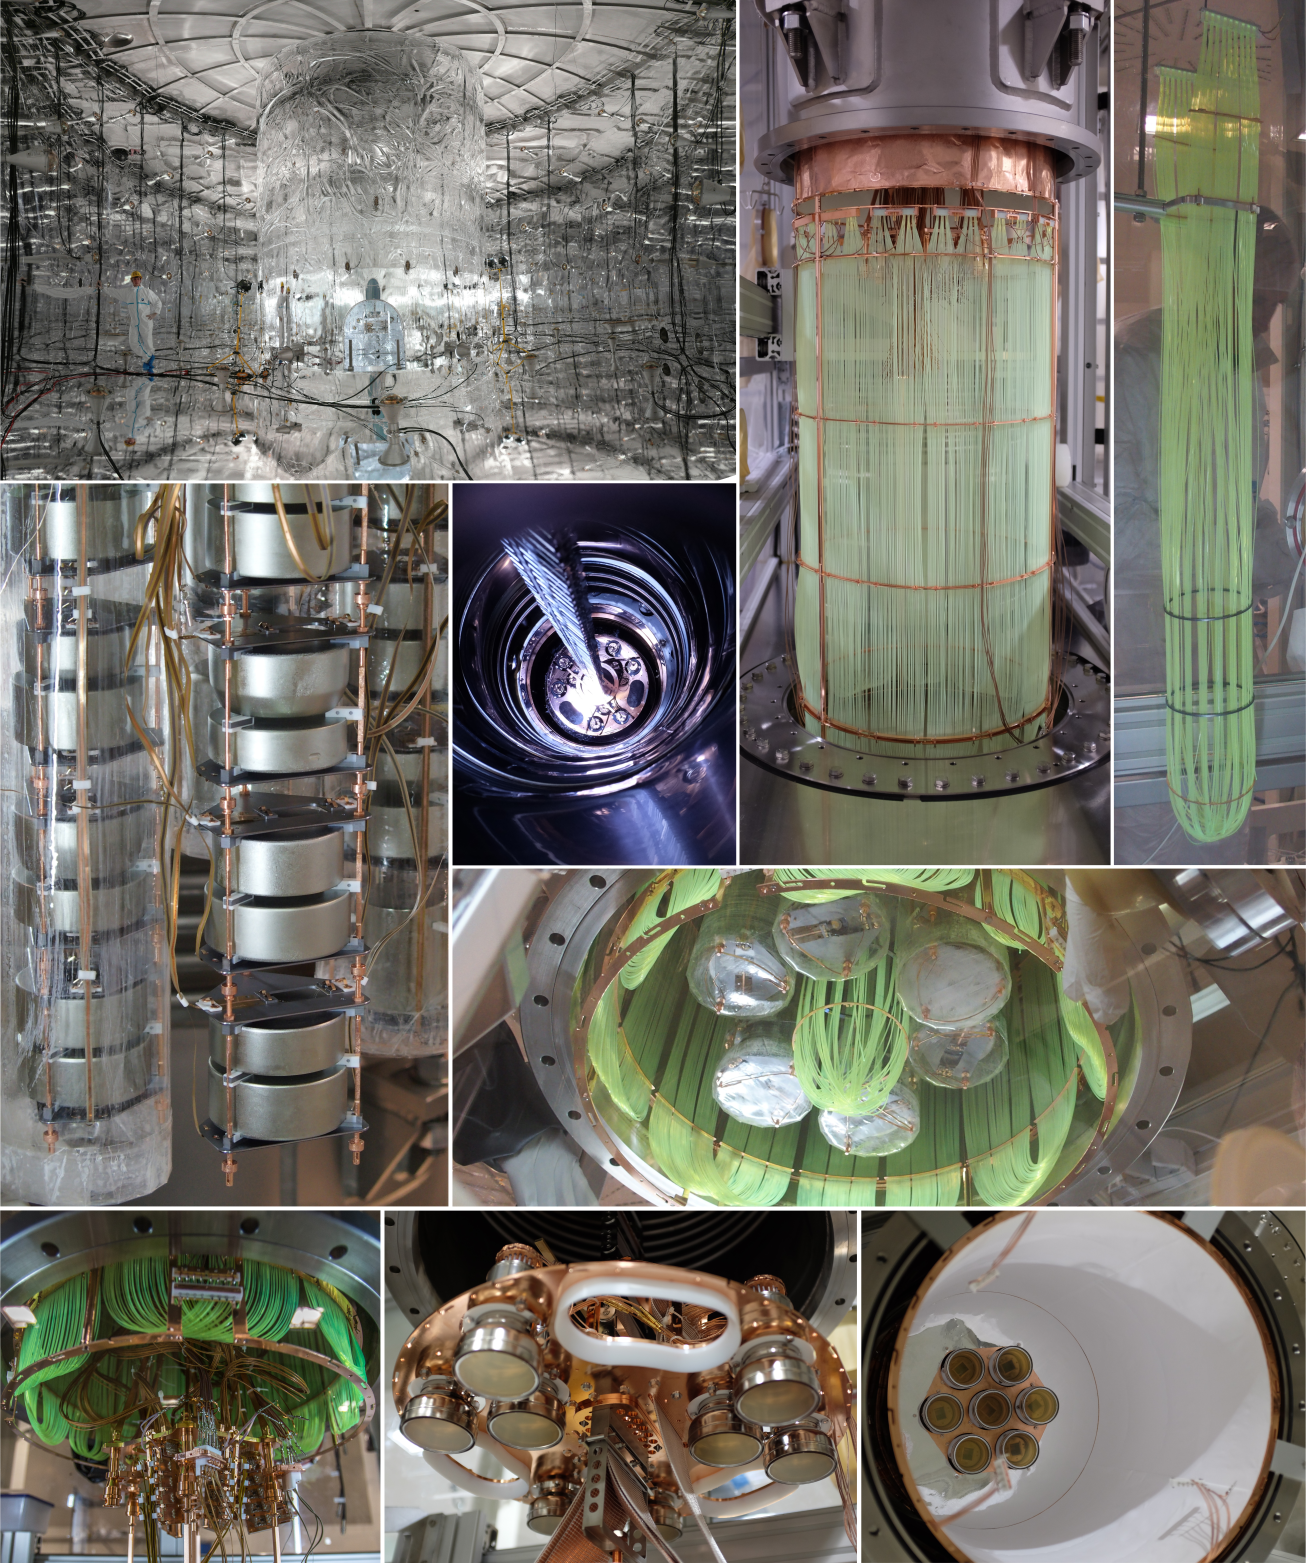
\includegraphics[width=\textwidth]{setup/pic-collage.png}};
    \node[label] at ( 0.3, 17.3) {\emph{a}};
    \node[label] at ( 8.7, 17.2) {\emph{b}};
    \node[label] at (12.8, 17.2) {\emph{c}};
    \node[label] at ( 0.3, 11.8) {\emph{d}};
    \node[label] at ( 5.4, 11.9) {\emph{e}};
    \node[label] at ( 5.4,  7.5) {\emph{f}};
    \node[label] at ( 0.3,  3.6) {\emph{g}};
    \node[label] at ( 4.7,  3.6) {\emph{h}};
    \node[label] at (10.0,  3.6) {\emph{i}};
  \end{tikzpicture}
  \caption{%
    Various pictures of the \gerda\ \phasetwo\ setup, taken during the upgrade works.
    \emph{a)} the muon veto instrumentation inside the water tank; \emph{b)} the light
    guiding outer fiber shroud; \emph{c)} the central fiber shroud; \emph{d)} \phasetwo\
    array closeup, \bege\ detector strings with their holder mounting and WLS mini-shroud
    are visible; \emph{e)} the array being lowered into LAr; \emph{f)} the end cap of the
    central fiber shroud is visible from below the assembled array; \emph{g)} the
    electronics front-end; \emph{h)} the top PMTs and holes for calibration sources;
    \emph{i)} the bottom PMTs in the Tetratex\reg-coated copper shroud.
  }\label{fig:setup:pictures}
\end{figure}

\blocktitle{calibration \\ system}
The \gerda\ weekly calibrations are performed by lowering three \Th\ sources into LAr in
the close vicinity of the array, at the same radial distance from the array central axis
and evenly spaced. Each source, when lowered, just fits into the space between the
cylinder of the LAr veto system and two neighboring outer strings of the detector array,
thereby the sources enter the inner volume of the LAr veto system by three slots in the
top PMT plate.  Three sources were produced and characterized for the first part of
\phasetwo~\cite{Baudis2015} and then again for \phasetwop. The LAr veto instrumentation is
usually switched off during calibration runs because of the too high source activity of
$\mathcal{O}(10)$~kBq.  However, less intense \Ra\ sources are also available and can be
easily exchanged with the standard ones. Special calibration data has been acquired with
these sources and the LAr light instrumentation turned on, to study the performance of the
LAr veto system. The calibration of the experimental setup is extensively described
in~\cite{calib-paper}.

\blocktitle{data \\ acquisition}
A FADC system records traces from germanium detectors (40), PMTs (16) and SiPMs (15) of
the LAr veto, PMTs and scintillating panels of the muon veto when an energy deposition
greater than about 100~keV occurs in at least one of the germanium detectors\footnote{The
  exact trigger threshold is detector- and run-dependent and varies between 20~keV and
200~keV.}. Besides of real physical triggers, two special artificial events are recorded
by the DAQ: test signals injected with a pulser in each germanium detector and baseline
events with no physical trigger to study the electronic noise. These events are recorded
at fixed time intervals during data taking. Since the outset, \gerda\ has adopted a
rigorous blind analysis strategy to ensure an unbiased search for \onbb\ decays. Events with
a reconstructed energy of $\qbbM \pm 25$~keV are blinded (i.e., removed from
the data stream) until the data selection is fixed.
\newpar
The energy deposition associated to each germanium detector signal is
determined via a Zero Area Cusp (ZAC) filter which is optimized off-line for each detector
and each calibration run~\cite{Agostini2015}. PMT and SiPM hits are reconstructed in the
offline analysis following the procedure documented in~\cite{Agostini2018a}. Each event
has to pass a series of quality cuts tailored to discard unphysical events with very high
efficiency (see \cref{sec:gerda:cuts}). The reconstructed trigger positions are converted
into time differences relative to the first trigger found in the germanium detector
traces. Trigger positions and amplitudes are subsequently used together with hits from the
SiPM to test the LAr veto condition. The algorithms were implemented in the \gelatio\
framework~\cite{Agostini2011} which is used to process \gerda\ data. Each event is
characterized by the calibrated energy deposited in the Ge diode, a data quality flag, the
classification as signal or background event from the pulse shape analysis, and veto flags
from the muon veto and LAr veto systems.

\begin{figure}
  \centering
  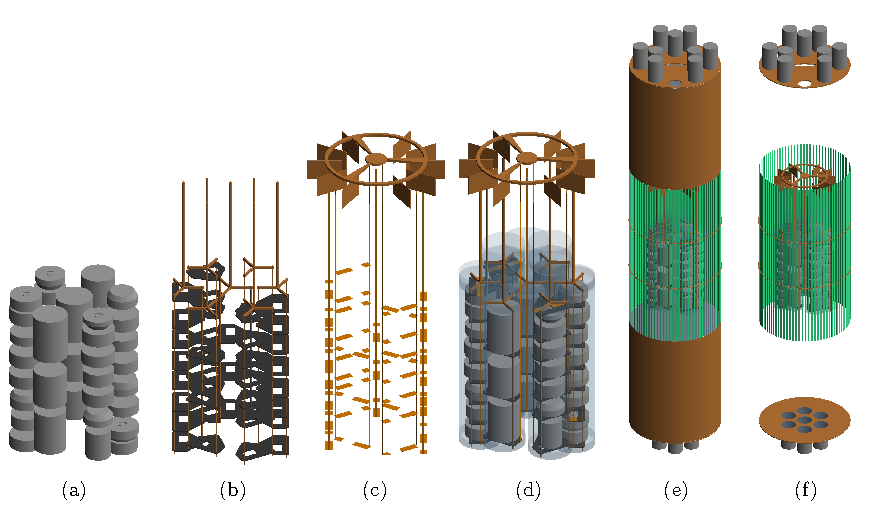
\includegraphics[width=\textwidth]{setup/mage-volumes.pdf}
  \caption{%
    Implementation of the \gerda\ array in \mage, visualized using the \geant\
    visualization drivers. From left to right: \emph{a)} the \phasetwo\ holder mounting,
    composed of silicon plates and copper bars, and the high-voltage and signal flex flat
    cables.  Front-end electronics are on the top end, \emph{b)} the full \phasetwo\ array
    instrumentation, including the transparent nylon mini-shrouds, \emph{c)} the full
    \phasetwop\ array instrumentation, including the central fiber shroud (in green),
    \emph{d)} the full \phasetwo\ LAr veto system, including the outer fiber shroud, the
    Tetratex\reg-coated copper shrouds (above and below the fibers) and the two PMT
    arrays, \emph{e)} the \phasetwop\ LAr veto system without the copper shrouds.
  }\label{fig:setup:magevolumes}
\end{figure}

\section{Background reduction techniques}%
\label{sec:gerda:cuts}

\begin{figure}
  \centering
  \includegraphics[width=\textwidth]{gedet/gerda-events.png}
  \caption{%
    Signal and background events in \gerda, working principles of the main background
    reduction techniques. From left to right: \emph{signal-like events}: the point-like
    topology in dense detectors of double-beta decays generate distinct single-detector
    pulse shapes. \emph{granularity cut}: external, background \g{}s can deposit energy
    in multiple detectors. \emph{pulse-shape discrimination}: insights on the event
    topology can be obtained by analyzing its waveform. Single-site events, multi-site
    events, \b{}s and \a{}s on the surface can be discriminated with offline algorithms
    depending on the specific detector geometry. \emph{LAr veto}: background events that
    deposit energy in germanium and LAr at the same time can be efficiently vetoed by
    the \gerda\ LAr veto.
  }\label{fig:gerda:event-types}
\end{figure}

Various background mitigation techniques are adopted, both at the data acquisition level
(online) and the analysis level (offline) in \gerda\ to lower the background index to the
background-free level of \pIIbi. The techniques outlined in the following have been
gradually developed and refined during several years of research and publications, and
have been employed for the \phasetwo\ final (re-)analysis in~\cite{gerda-final}.
Documentation about partial analyses of the \gerda\ \phasetwo\ data published
in~\cite{Agostini2015a, Agostini2017, Agostini2018, Agostini2019a} can be found in those
publications and references therein.

\blocktitle{muon veto}
Muons may cause a substantial background to rare event searches like \gerda\ by generating
counts at \qbb\ either through direct energy deposition in the detectors or through
e.g.~decay radiation of spallation products. At LNGS the cosmic muon flux is reduced by a
factor of ${\sim}10^6$ to a rate of ${\sim}3.4 \cdot 10^{−4}~\text{s}^{-1}\text{m}^{-2}$,
which is sill sufficient to generate a non-negligible background of the order of
\powctsper{-3}.  As already described in \cref{sec:gerda:setup}, a muon veto comprising of
a water \v{C}erenkov veto and a scintillator veto was implemented in \gerda\ to reduce
this background contribution. An event with energy deposition in germanium is flagged
as muon-induced background if a coincidence with the muon veto signal occurs in a $\pm
10$~\mus\ window around the germanium trigger. The efficiency of the muon veto system
has been estimated to be of ${\sim}99$\%, leading to a residual background index of
${\sim}$\powctsper{-5}~\cite{Freund2016}.

\blocktitle{LAr veto}
The primary role of liquid argon in \gerda\ is to keep the germanium detectors at a
cryogenic operational temperature and provide a passive shielding medium against external
backgrounds. Moreover, the LAr can be also employed as a detector medium in an active veto
system, thanks to its scintillation properties. The production mechanism of the
scintillation light in LAr is known since several decades and is deeply described in
literature and its spectrum is today well known. The incident particles deposit their
energy mainly by interactions with the electron shell of the argon atoms which leads to
either an excitation or an ionization of argon atoms. Excited argon atoms are frequently
called `excited dimers' or `excimers' in the literature. Their decay is accompanied by the
emission of scintillation light in the vacuum ultraviolet region, whose typical wavelength
is usually cited as $\lambda = 128$~nm~\cite{Heindl2010}. The ratio between excitation and
ionization is strongly dependent on the pressure and density of the argon as well as on
the type of radiation itself. In the case of excitation, the excited argon atom can
directly form an excimer via the collision with neighboring argon atoms. The process is
sketched in \cref{fig:setup:lar-scint}.
\begin{figure}
  \centering
  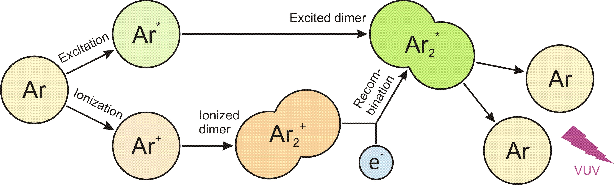
\includegraphics[width=0.7\linewidth]{lar-scint-mechanism.pdf}
  \caption{%
    Scintillation mechanism of liquid argon (or gaseous argon) via the decay of excited
    dimers. The excited dimer can be either formed directly from an excited argon atom or
    from an ionized atom which forms an ionized dimer before its recombination and the
    following recombination in its molecular form. Drawing courtesy of Christoph
    Wiesinger.
  }\label{fig:setup:lar-scint}
\end{figure}
The excimer itself is meta-stable and appears in two different states: the singlet and the
triplet state~\cite{Jortner1965, McCusker1984}.  The decay of the triplet state is
forbidden due to angular momentum conservation, while the decay of the singlet state is
allowed. Consequently the lifetime of the triplet state is 1.59~\mus\ which is
significantly higher than the 6~ns of the singlet state. The scintillation light yield
(combined for both components) is roughly 40 photons/keV, measured in ultra-pure
LAr~\cite{Doke1988}. This value is dependent on different factors, like the presence of
contaminants, the pressure and density of the argon as well as the ionization density of
the incident particle~\cite{Doke1988}.
\newpar
The goal of the \gerda\ LAr veto is to reject those types of background events in the
germanium detectors that simultaneously deposit energy in the surrounding LAr, and hence
generate scintillation. These background types mainly include \g-ray background from Ra
and Th decays in solid materials inside and around the detectors. But also other types of
background can successfully be rejected, such as muons or decays from \Arh\ or \kvz. An
event depositing energy in the germanium detectors is discarded as background if a
coincidence with the LAr veto signal is found in the time window spanned by the germanium
traces.  Since the lifetime of the LAr triplet state significantly depends on the argon
purity~\cite{Amsler2007}, it is possible to monitor the purity of LAr over time.
\cref{fig:lar:triplet-lifetime} shows the lifetime values measured about every month since
the start of \phasetwo. The average measured lifetime dropped after the \phasetwop\
upgrade works from $\sim$1~\mus\ to $\sim$0.9~\mus, as a probable consequence of
maintenance works of the cryogenic system.
\begin{figure}
  \centering
  \includegraphics{plots/lar/lar-triplet.pdf}
  \caption{%
    LAr triplet lifetime regularly measured during \phasetwo. The decrease of the LAr
    purity in 2018 might be attributed to maintenance works of the cryogenic
    infrastructure.
  }\label{fig:lar:triplet-lifetime}
\end{figure}
The veto condition is realized when the signal in at least one channel (SiPM array or PMT)
exceeds a certain threshold (around one photo-electron or less) within a certain time
window around the germanium trigger (usually few microseconds). The \onbb-signal
efficiency of the LAr veto cut can be estimated by evaluating the number of test pulses
and baseline events that are randomly flagged as background events. This fraction has been
evaluated to $(97.7 \pm 0.1)$\% and $(98.2 \pm 0.1)$\% for the first part of \phasetwo\
and \phasetwop, respectively. Combining these two estimates for the whole \phasetwo\
results in an efficiency for \onbb\ events of
\[
  \epsilon_\onbbM^\text{LAr-veto} = \fillme{fillme} \;.
\]

\blocktitle{granularity \\ cut}
Since the topology of \onbb-decay events in germanium is, to a good approximation,
point-like, all events in which energy is simultaneously deposited in more than one
detector can be classified as background. In the offline analysis of a physical event, a
trigger algorithm is applied over all the germanium traces to determine the presence of
other signals besides the main trigger. This `offline' trigger threshold can be as low as
the electronic noise and accounts for possible electronic crosstalk effects between
channels.

\blocktitle{data \\ quality}
Each event has to pass a series of quality cuts tailored to discard unphysical events such
as discharges, pile-up, overflowed events and other problematic traces with very high
efficiency. The \onbb-signal efficiency of the data quality cuts has been estimated by
building an artificial signal-like data sample and applying the data quality cuts to it.
The base for this data sample consists of special pure-baseline events without physical
triggers, which are regularly recorded in \gerda. Since these events are artificially
triggered, no signal is expected in any detector with high probability, and therefore they
can be used to characterize the background noise at a given time during data taking. On
top of these baseline events special averaged waveforms from \Th\ DEP events are added to
baseline events (only one channel per event) to produce the signal-like sample. An
estimation of the acceptance of these events is finally yields:
\[
  \epsilon_\onbbM^\text{QC} = (99.922 \pm 0.002)\% \;.
\]

\blocktitle{pulse-shape \\ discrimination}
The drift of charges created by a ionizing particle in a voltage-biased germanium
detector, which determines the shape of recorded event waveform, depends on the electric
field in the diode. The latter, in particular, depends on the geometry and on crystal
parameters like the impurity concentration and its gradient. Therefore, analysis
techniques can be developed to discriminate between various event types in germanium
detectors. Distinguishing between single-site (SSE) and multi-site (MSE) events is of
primary interest for \gerda, since \onbb\ decays pertain to the SSE class. The two
electrons, in fact, deposit their energy in germanium within 1~mm$^3$ and can be therefore
considered as point-like events. On the other hand, background events caused by
e.g.~multiple Compton scattering of external \g\ rays are mostly of the multi-site type.
Besides MSEs, surface events are another prominent source of background. Energetic \b\
rays created at the \nplus\ electrode surface can penetrate the dead-layer and deposit
energy in the active volume. In particular, the \b\ decay of \kvz, a daughter of \Arh\
naturally present in LAr, is a dangerous background in the ROI because of its high
Q-value. These \b\ decays at the \nplus\ surface can create `slow' pulses with incomplete
charge collection because of the low electric field in the Li-diffused region. The \pplus\
electrode and the insulating groove can be trespassed also by \a\ particles. The
shallowness of the boron implantation of the \pplus\ (hundreds of nanometers) and the
absence of any dead layer in the groove\footnote{The passivation layer, if present, is
usually hundreds of nanometers thick and can be therefore penetrated by \a\ particles.}
let external \b{}s and \a{}s deposit energy in the detector active volume. The intense
electric field causes energy depositions in this region to generate pulses with short
rise times. \a\ events on the \pplus\ electrode are mainly produced by \Po\ accumulated
on its surface, most probably during detector handling. These 5.3~MeV \a\ particles may
lose part of their energy before reaching the active volume and contribute to the
background in the ROI.
\newpar
To mitigate all these background sources, pulse-shape discrimination (PSD) techniques were
developed separately for \bege\ and \scoax\ detectors separately, to be applied after the
LAr veto cut. For the first class a simple univariate cut was sufficient, while for the
latter two techniques were worked out, one based on neural networks and one on the
analysis of the rise time of the pulses.  In order to avoid systematic effects
calibration, training and evaluation of the PSD methods should be performed on pulses with
energies close to these of the expected signal at \qbb.  In practice, appropriate event
sets are extracted from the weekly \Th\ calibration spectra. The PSD methods applied to
the \gerda\ data are briefly outlined in the following. The interested reader is referred
to~\cite{psd-paper} for a detailed treatment of the topic. \fillme{define somewhere FEP,
SEP and DEP}

\blocktitle{PSD for \\ \bege{}s}
PSD for the \bege\ detectors is based on the \aoe\ ratio, where $A$ is the maximum
amplitude of the current signal and $E$ is the event energy. This technique has been
extensively studied in the past in the context of \gerda~\cite{Agostini2013, Agostini2010,
Budjas2008, Budjas2009, Budjas2009a, Agostini2010a}. The motivation in employing such a
relatively simple, univariate cut lies in the observation that in the \bege\ detectors,
thanks to their small \pplus\ contact, the electric field has a special distribution,
resulting in the same shape of pulses induced by drifting holes along paths near the
\pplus\ electrode~\cite{Agostini2010}. Multiple energy depositions in the detector can be
treated as a superposition of several single interactions. It follows that a MSE will have
a lower $A$ compared to a SSE with the same $E$.  A two-sided cut on \aoe\ to cut MSEs
slow pulses and \pplus\ fast events is introduced and determined separately for each
detector. Energy and time stability corrections to \aoe\ are discussed in detail
in~\cite{psd-paper}. As mentioned before, the \aoe\ cut values are determined employing
representative data samples from \Th\ calibration runs.  The low cut position (rejection
of MSEs and slow pulses) is adjusted to achieve a 90\% survival fraction of the
double-escape peak (DEP), a SSE sample. The threshold on the high \aoe\
side (rejection of fast pulses) has been fixed to 3 standard deviations away from the SSE
band distribution. The survival fraction for the \onbb-decay signal has been
calculated assuming that it is the same as for the DEP events. A full analysis of the
statistical and systematic uncertainties yields:
\[
  \epsilon_\onbbM^{A/E} = (87.6 \pm \stat{0.1} \pm \syst{2.6}) \% \;.
\]

\blocktitle{PSD for \\ \scoax{}s}
In semi-coaxial detectors the length of the drift path of the holes depends on the
location of the energy deposition and it induces different types of pulse shapes. Because
of this reason, a simple \aoe\ cut would not be as effective as for the \bege{}s, and
therefore alternative methods have been worked out.
\newpar
The primary method to reject MSE, called here \annmse, consists in a TMVA-based
artificial neural network\footnote{\url{https://root.cern/tmva}} and requires
appropriate selection of input variables (from the rising part of the preamplifier charge
pulse) and training on independent data samples. Several of these samples are available
for training in calibration data (see \cref{fig:gerda:calib-desc}, top) and also in physics data (\kvz\
full-energy peak, \nnbb\ events, \a-induced events). The \annmse\ is specifically trained
on \Th\ calibration data, selecting the \Tl\ DEP as a SSE sample and the \Bil\ FEP at
1621~keV as a MSE sample. The classifier cut threshold is then fixed to a 90\% survival
probability for the \Th\ DEP, and the cut signal efficiency is calculated from Monte Carlo
simulations of \onbb-decay events. The obtained \annmse\ signal survival fraction is $(85
\pm 5)$\%.
\newpar
\a-induced events on the \pplus\ electrode surface are rejected by a separate method based
on the analysis of the pulses rise time (RT). These events are generally characterized by
a fast collection time, and their charge collection might be delayed or partial, if
originated in the proximity of the groove. The RT cut exploits the fast rise time of these
\a\ events and is therefore equivalent to a volume cut, which excludes the surfaces
vulnerable to the \a-induced events. The rise time is defined as the time the waveform
needs to reach from 10\% to 90\% of its amplitude. The RT-cut threshold is defined to
maximize the \onbb\ survival fraction and to minimize the signal-to-noise ratio at the
same time through the definition of a figure of merit defined as the product of the \nnbb\
signal survival square-probability and the \a-events rejection probability. The \nnbb\ and
\a-event test samples are obtained from physics data by selecting data in the $[1.0,
1.3]$~MeV and $>3.5$~MeV energy regions, respectively, after \annmse\ and LAr veto cuts.
The \onbb-signal efficiency of the RT cut is assumed to be the same as for the \nnbb\
decays and hence estimated to $(84.3 \pm \stat{0.4} \pm \syst{1.0})$\%. The \annmse\ and
RT-cut efficiency can be combined to obtain an overall survival fraction for the
\onbb-decay events after the combined \annmse-RT cut:
\[
  \epsilon_\onbbM^\text{\annmse-RT} = (64.6 \pm 3.9) \% \;.
\]

\blocktitle{\deltae\ cut}
Events featuring slow charge collection might suffer from ballistic deficit in the ZAC
energy reconstruction~\cite{Agostini2015} and survive the PSD cuts, especially in
semi-coaxial detectors. Therefore an additional rejection criteria is applied based on the
energy reconstructed with different integration times. The figure of merit for such a cut
is the ratio between the energy of an event reconstructed with a short (4~\mus)
integration time $E_\text{s}$ and the energy reconstructed with a long (20~\mus)
integration time $E_\text{l}$. The energy here is reconstructed using a gaussian-shaping
filter, which has been the default \gerda\ energy reconstruction method for \phaseone.
Ballistic deficit is observed to reduce this ratio, therefore the \deltae\ classifier is
defined as $\delta{E} = {[E_\text{s}/E_\text{l}]}_\text{norm} - 1$, where the energy ratio
is normalized to the values assumed by the \Th\ FEP events. The normalization is applied
in a certain calibration validity period and for each detector separately. The cut value
is defined as 3 negative standard deviations away from the mean of the FEP \deltae\
distribution.

\section{Data analysis}%
\label{sec:gerda:ana}

The \phasetwo\ single-detector data is presented in this section together with the LAr
veto and PSD data.  The statistical analysis used to extract a lower limit for the \onbb\
half-life in \gesix\ is finally presented, and the final results for the combined \gerda\
data are given.

\begin{figure}
  \centering
  \includegraphics{plots/0nbb-results/calib/supercalib.pdf}
  \caption{%
    Top panel: \Th\ calibration summed spectra of \bege, semi-coaxial and inverted-coaxial
    detectors as used to determine the energy resolution curves. Three prominent \Tl\ high
    energy peaks (full-energy, single-escape and double-escape) and the \Bil\
    single-escape peak at 1621~keV are highlighted. Bottom panel: extracted peak widths
    and fitted calibration curves. Points represented by empty markers are excluded from
    the fit because of additional effects that contribute to the width. Triangles label
    peaks broadened by the Doppler effect \fillme{ref?}, diamonds label summation peaks.
    \fillme{fillme}
  }\label{fig:gerda:calib-desc}
\end{figure}

\blocktitle{energy \\ scale and \\ resolution}
As already emphasized in \cref{sec:nbb:exp}, a good energy resolution is a key ingredient
to achieve a high \onbb-decay sensitivity. The main goal of the calibration analysis is
therefore to define and maintain a stable energy scale over years of data taking.  It
is necessary to identify the peak region (and reject all background events with
different energy), combine data from different detectors over extended periods of time,
and efficiently exploit the excellent energy resolution of germanium detectors.
\newpar
As already mentioned in \cref{sec:gerda:setup}, the germanium detectors are calibrated by
exposing them to \Th\ sources with an activity of about 10~kBq. A typical calibration
spectrum is shown in \cref{fig:gerda:calib-desc}. The pattern of \g\ lines in the spectrum
can be exploited to identify certain \g\ lines and calibrate the energy scale of a
detector with their known position in terms of energy.  Additionally, the resolution of a
detector can be determined from the width of the \g\ lines. Once the positions and the
widths of the \g\ lines in an energy spectrum is determined by modeling the peaks with a
suitable analytical function, an function interpolation is performed to obtain the energy
calibration and resolution at other energies. Once these two curves are determined for a
given calibration, they are assumed to be valid until the next one. This validity is
constantly monitored by evaluating the shift of the pulser event energy over time with
respect to its value right after a calibration. Time periods in which in which a detector
shows deviations from its calibration above a certain threshold are removed from the final
analysis in order to meet the stringent requirements for the \onbb\ analysis in terms of
uncertainties on the energy scale and resolution. Fluctuations below this threshold are
taken into account when estimating the systematic contribution to the uncertainty on the
energy resolution. The stability of the energy scale and resolution is also monitored on a
per-calibration basis, and time periods for which detectors show a degraded performance
are excluded from combined analysis data sets.  The calibration spectra that refer to
these combined data sets are obtained by summing together the spectra from all the
calibration runs of the relative time period weighted by their actual validity in time.
Gaussian mixtures are usually not needed to model peaks in these combined spectra, as the
variance of the single centroids and widths is usually small enough to enable the use of
single gaussian distributions with effective parameters. The effective data set energy
resolution is then determined by fitting the square root of a linear function to the
reconstructed \g-line widths. The uncertainty on this effective resolution includes
systematic contributions from the choice of the peak model, the resolution function and
time stability of the experimental setup.  The resolution curves for \bege, semi-coaxial
and inverted-coaxial \phasetwop\ data sets are reported in \cref{fig:gerda:calib-desc} as
an example. The typical energy resolution at \qbb\ is \fillme{fillme} and the associated
uncertainty is of the order of \fillme{fillme}. The calibrated energy spectrum of the
\gerda\ \phasetwo\ data after granularity cut is shown in \cref{fig:gerda:spectrum-cuts},
empty histogram. \fillme{update this to final analysis, calibration paper?}

\begin{figure}
  \centering
  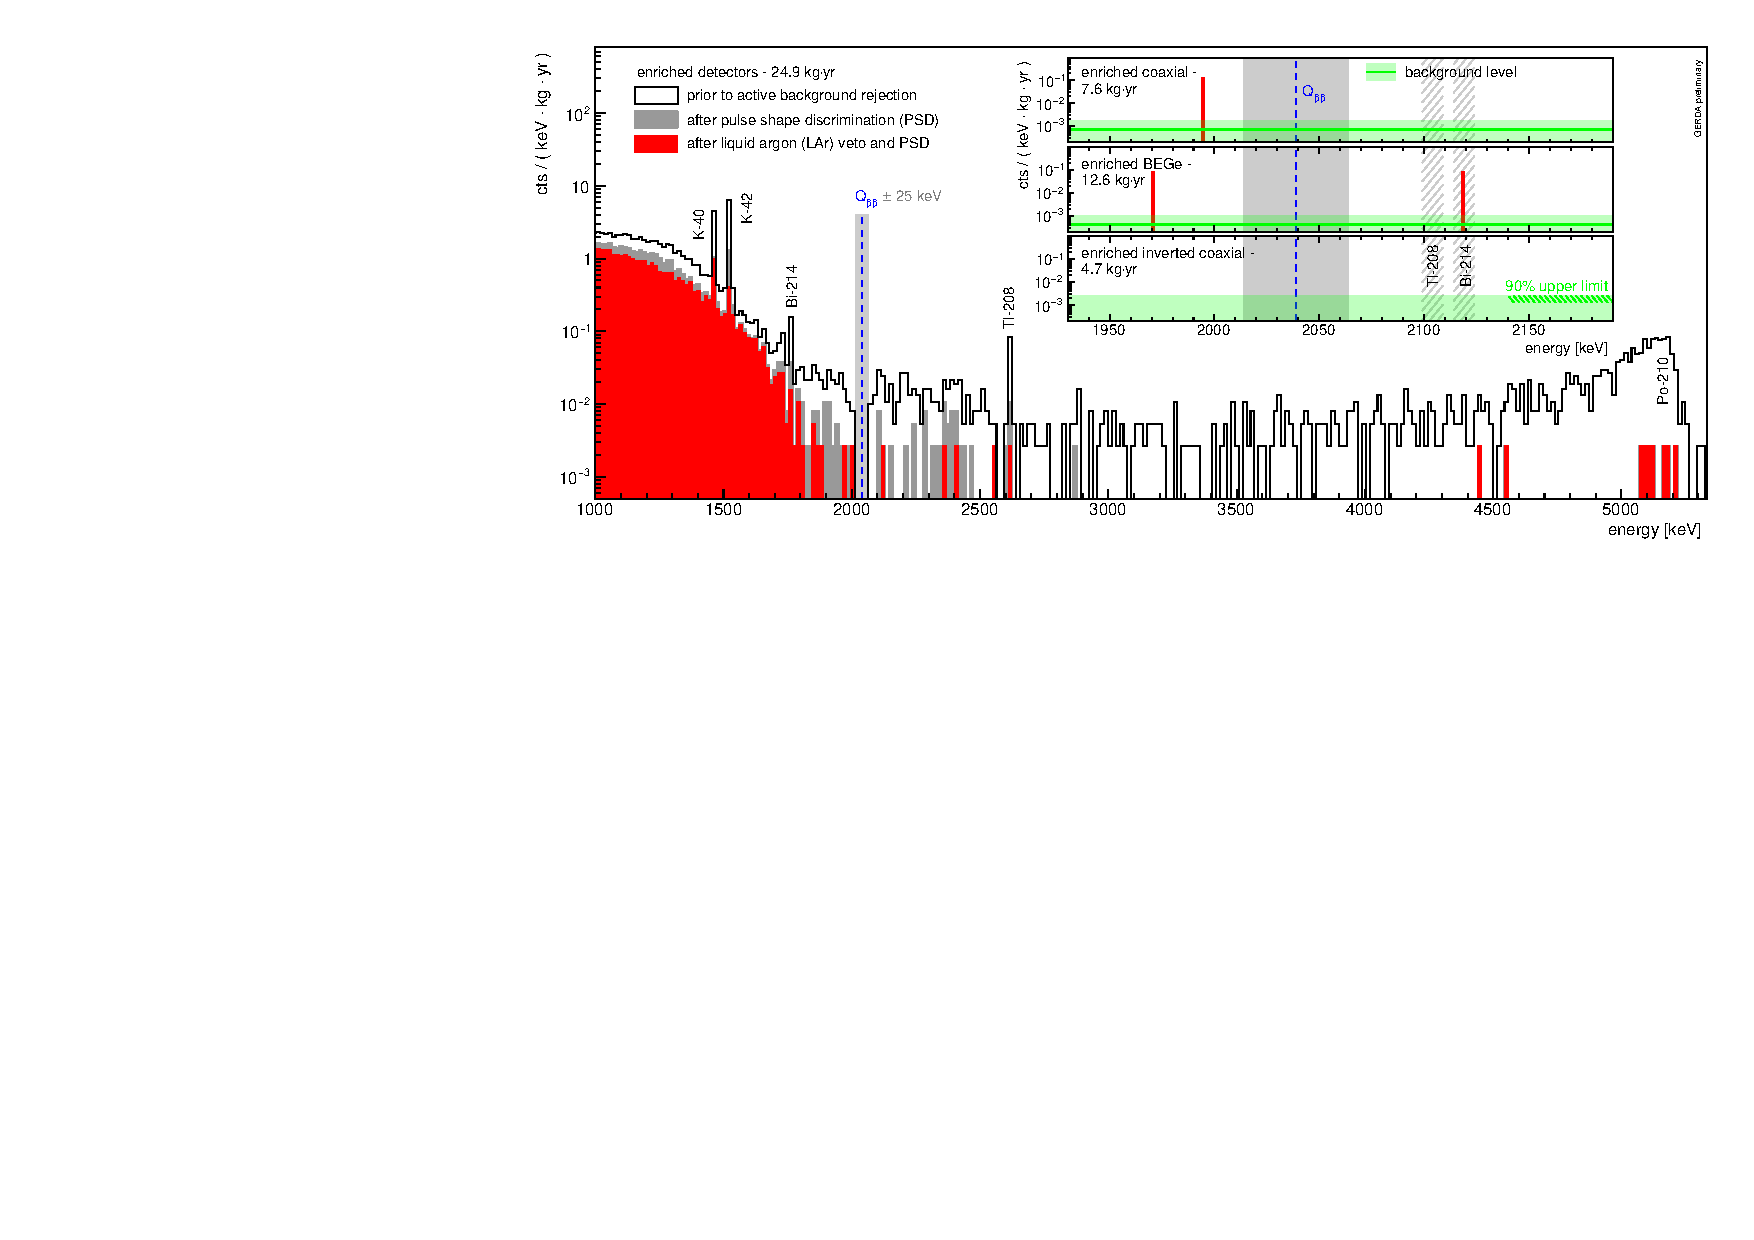
\includegraphics[width=0.9\linewidth]{plots/0nbb-results/spectrum-cuts.pdf}
  \caption{%
    Single-detector data from the enriched detectors is displayed in a combined spectrum
    after indicated cuts. Main contributions to the spectra are labeled. The insets
    display the analysis window for coaxial and \bege\ detectors separately, including the
    background rates (solid blue lines). The dashed blue curves depict the 90\% C.L.~limit
    for a \onbb\ signal of \gerdafinallimit. \fillme{to be updated}
  }\label{fig:gerda:spectrum-cuts}
\end{figure}

\begin{figure}
  \centering
  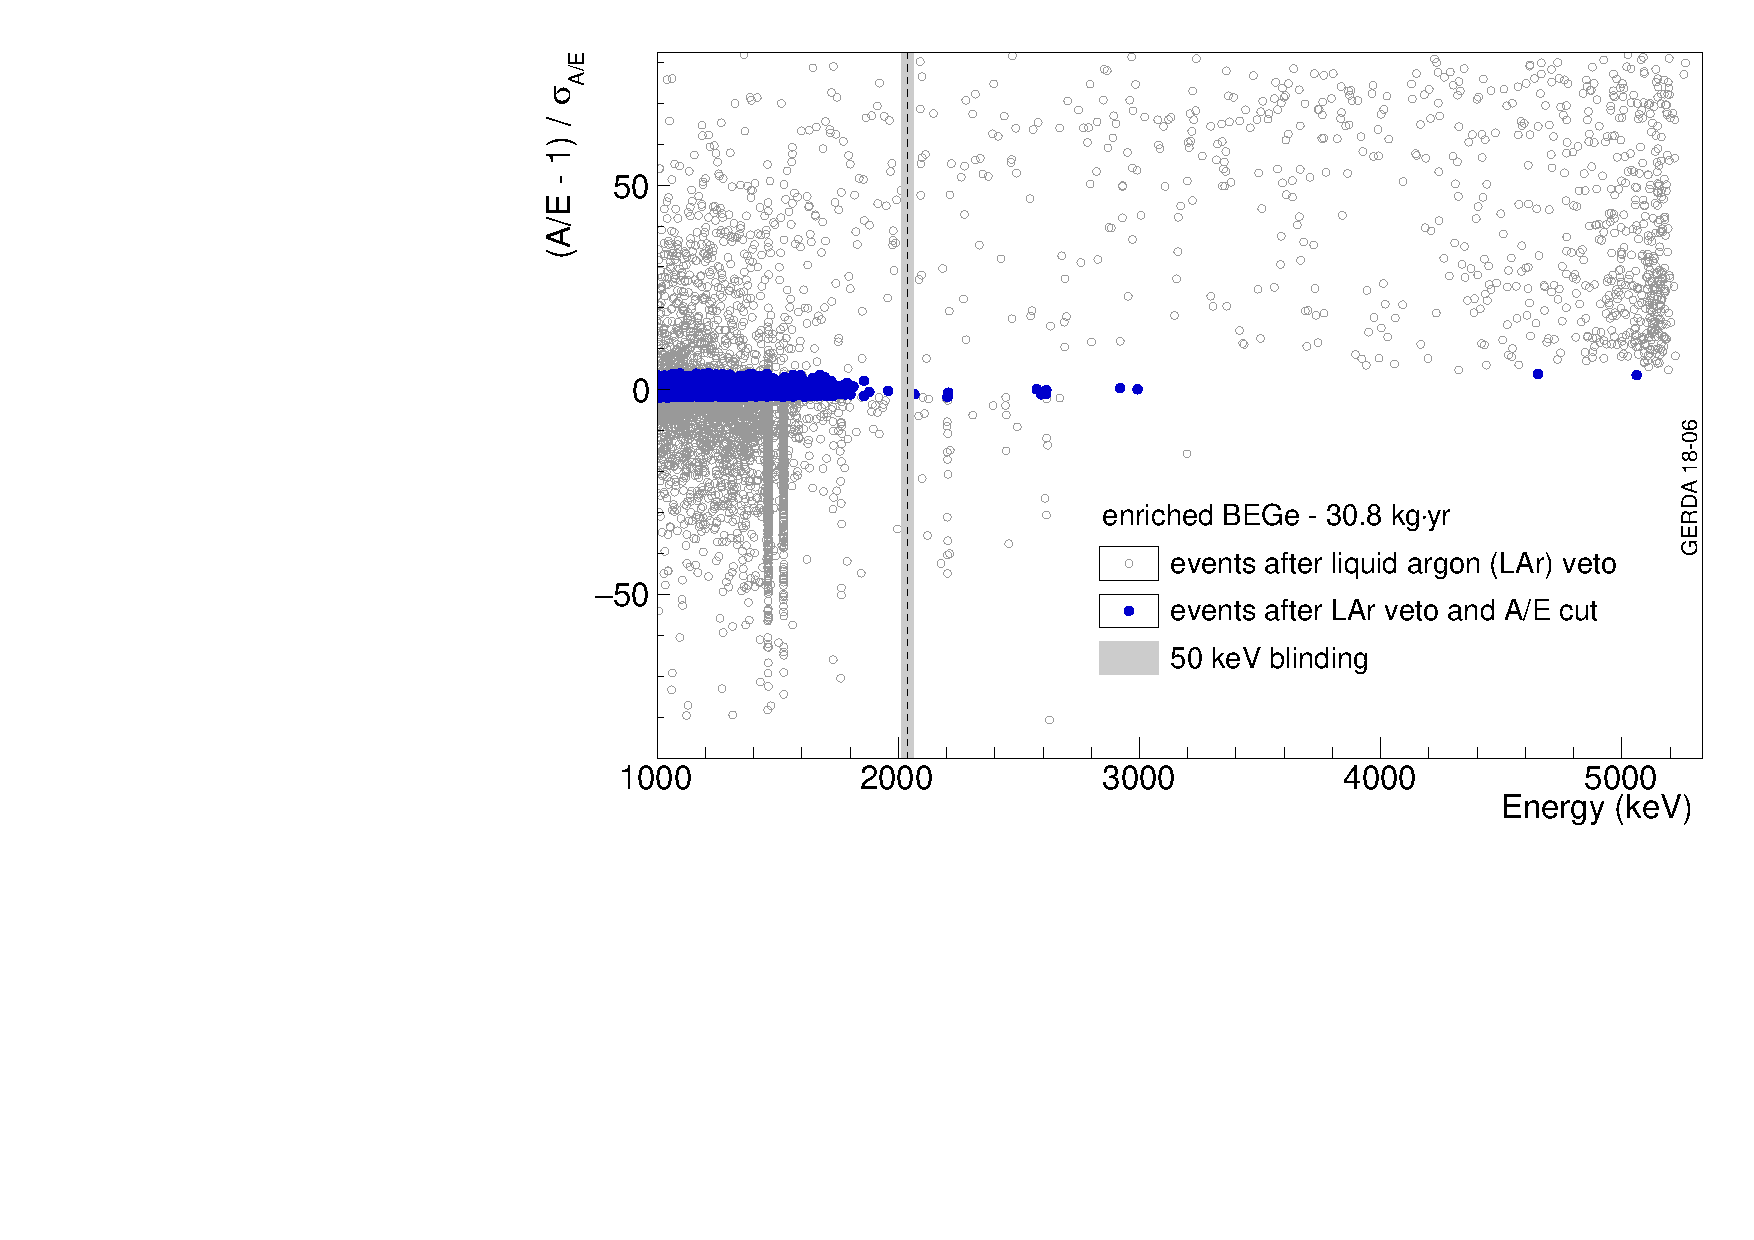
\includegraphics[width=0.45\textwidth]{plots/0nbb-results/aoe-on-data.pdf}%
  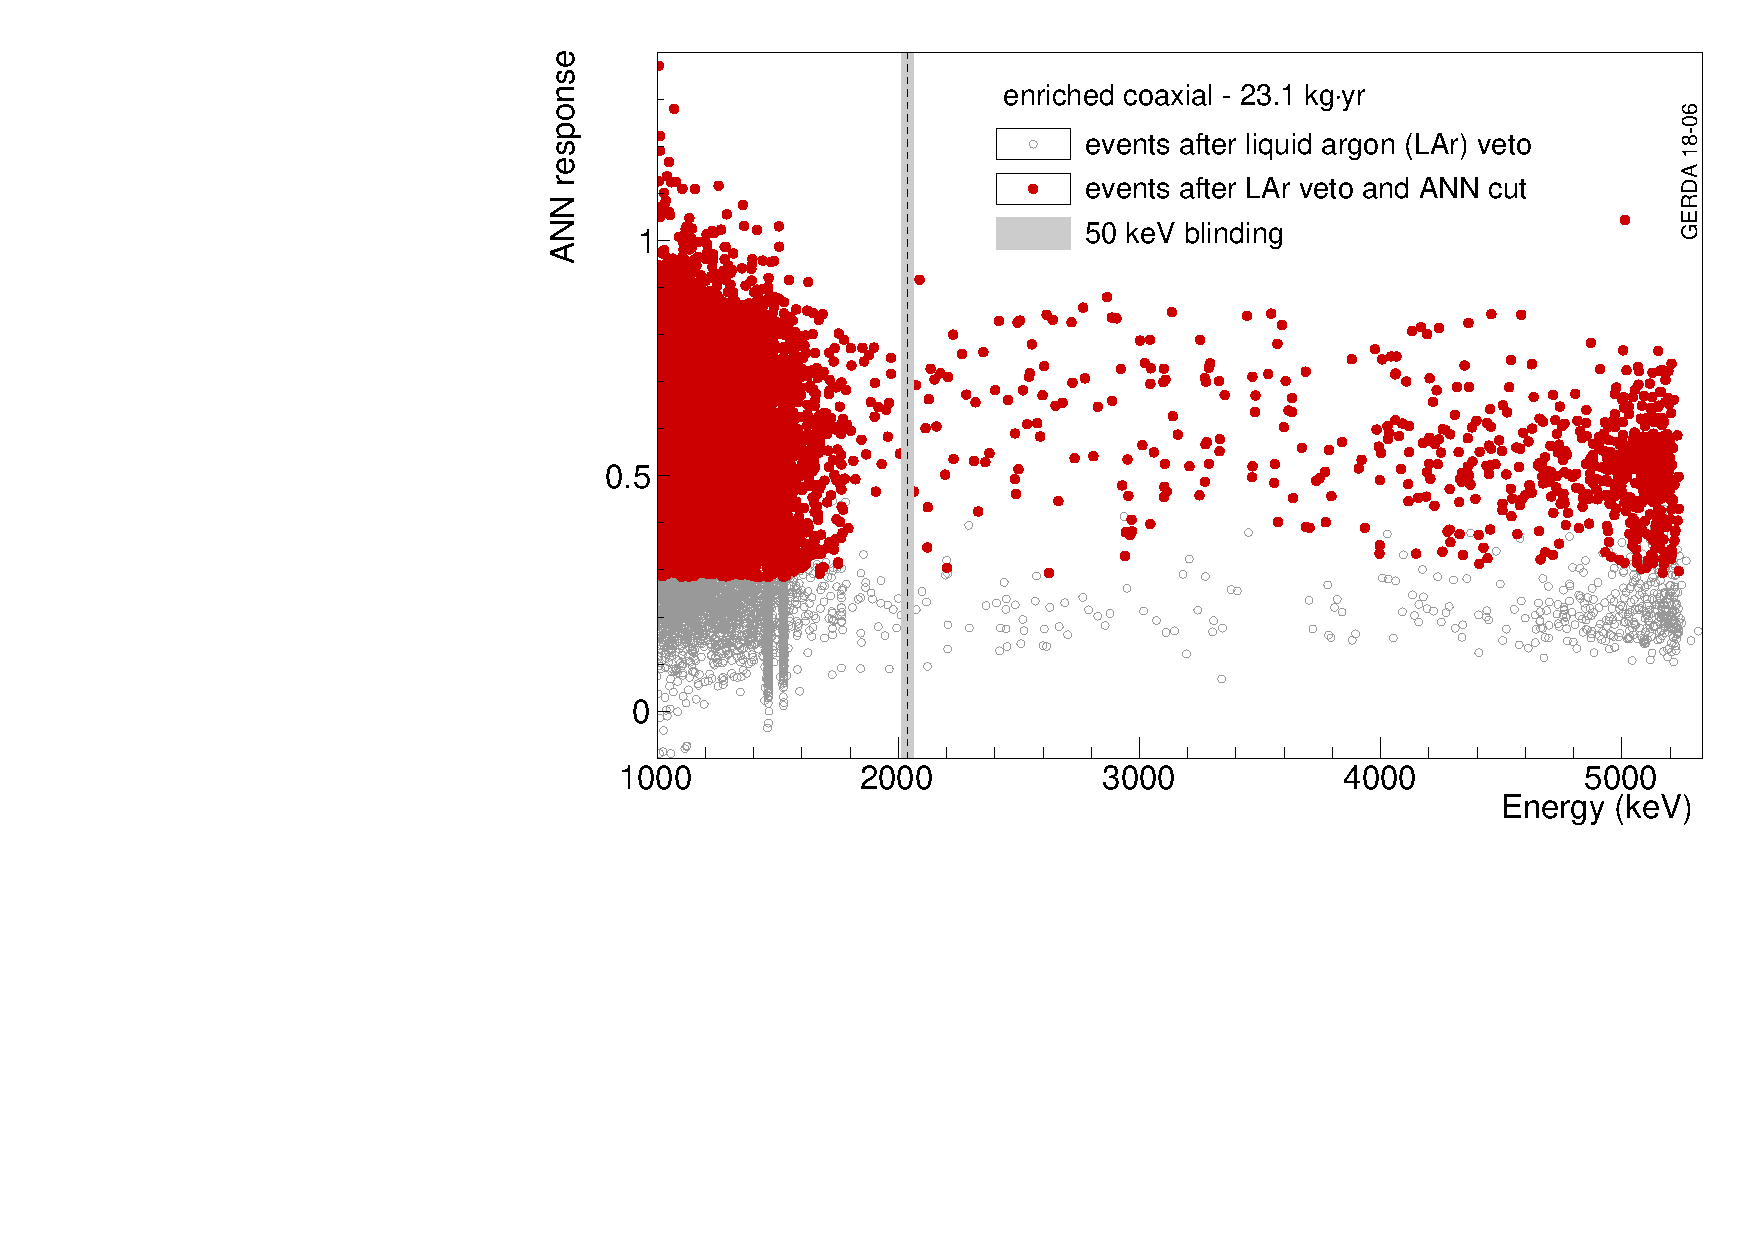
\includegraphics[width=0.45\textwidth]{plots/0nbb-results/ann-on-data.pdf}
  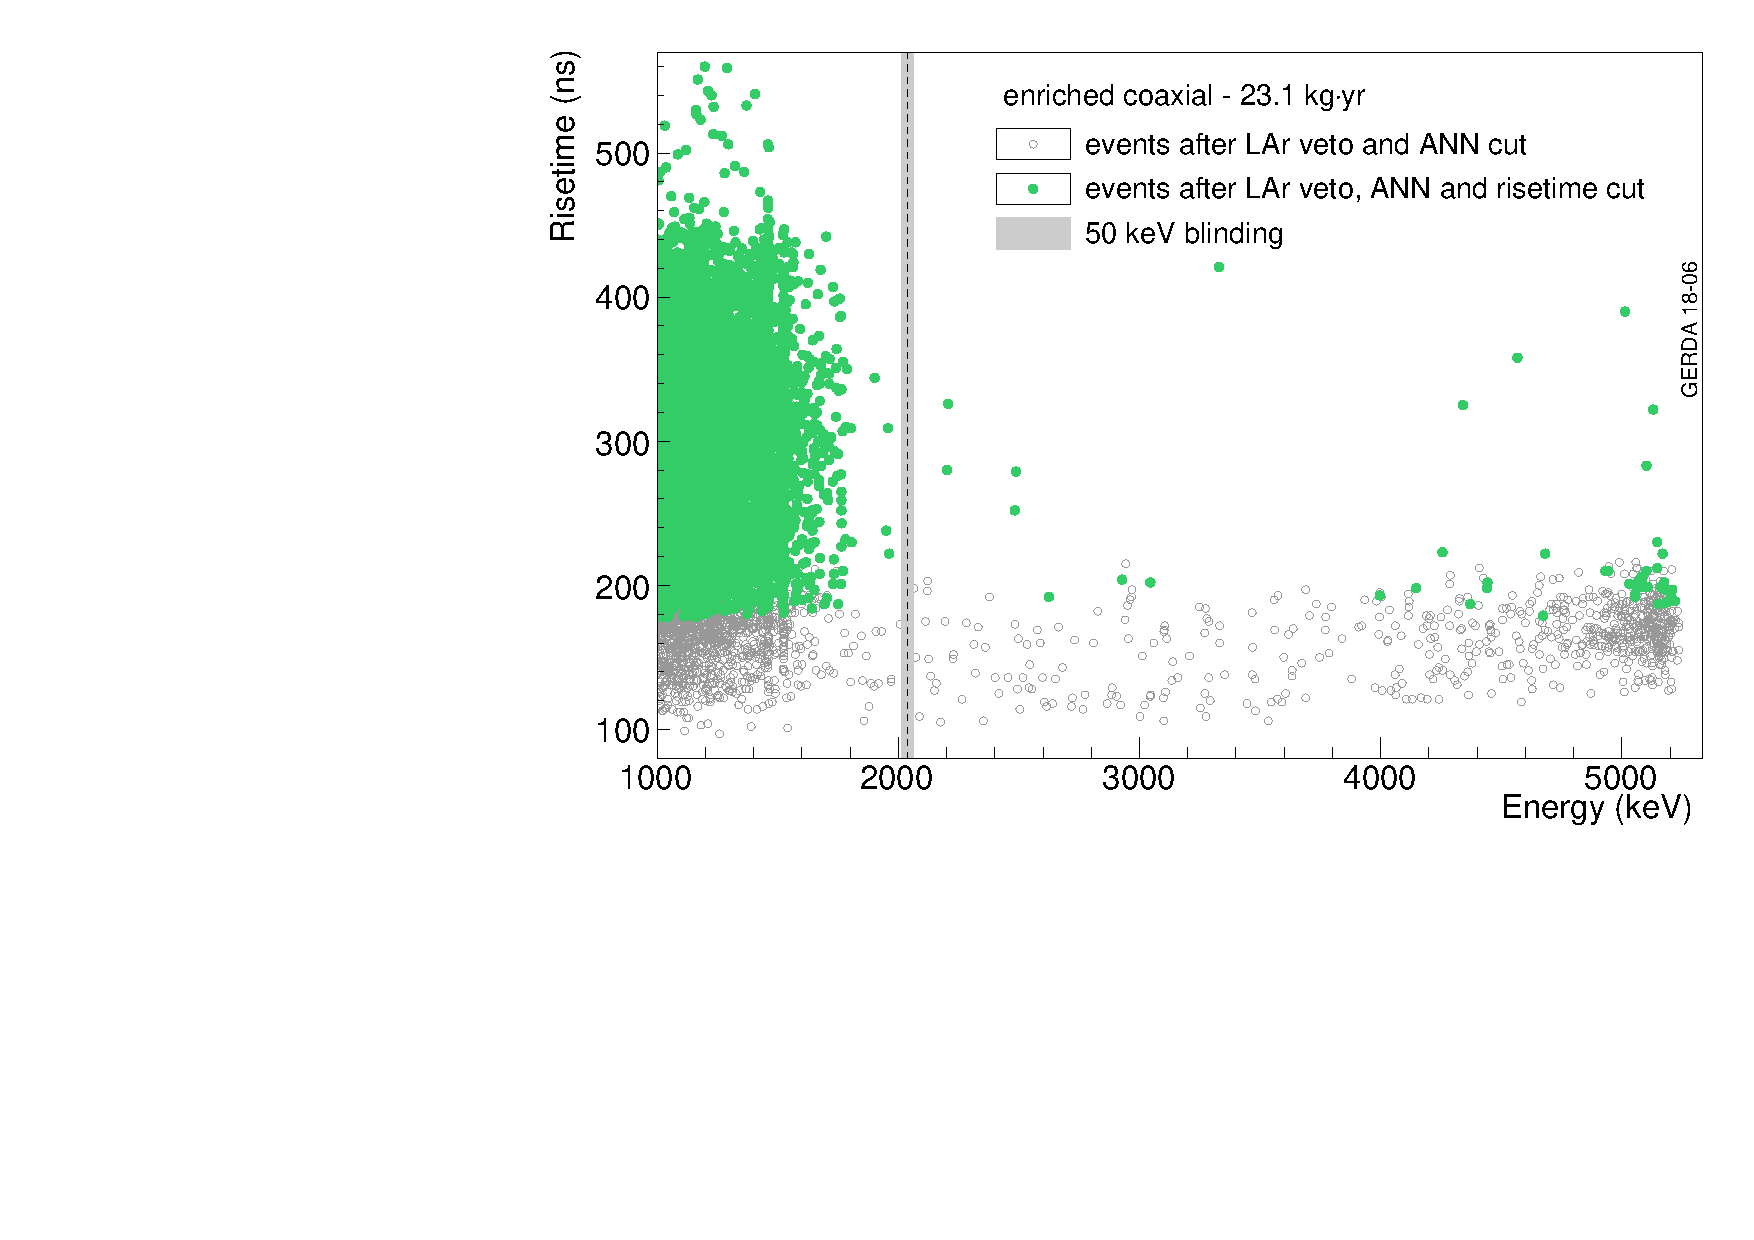
\includegraphics[width=0.45\textwidth]{plots/0nbb-results/rt-on-data.pdf}
  \caption{%
    The three pulse shape discrimination techniques applied on the \gerda\ \phasetwo\
    data. From left to right: the \aoe\ cut, the \annmse\ cut, the rise-time cut.
    \fillme{to be updated with full data}
  }\label{fig:gerda:psd-on-data}
\end{figure}

\blocktitle{statistical \\ methods}
\fillme{update to final decision}

\blocktitle{LAr veto and \\ PSD cuts on \\ data}
The first cut applied to \phasetwo\ data (after the quality cuts and the multiplicity cut)
is the LAr veto cut.  Event energy histograms before and after this event selection are
shown in \cref{fig:gerda:spectrum-cuts}. The cut clearly suppresses background events from
the \Th\ and \Uh\ decay chains, as well as \kvz\ events. The \kvz\ FEP event reduction to
20\% and 18\% in \phasetwo\ and \phasetwop\ data, respectively, demonstrates the
effectiveness of the improved fiber instrumentation installed for \phasetwop. \kvn\
events, which are characterized by a single \g\ emission at 1461~keV and typically do not
deposit energy in LAr, show a high survival fraction of about 98\%, but cannot enter the
ROI at 2039~keV and are therefore of minor concern. \a\ events that dominate the energy
spectrum at higher energies cannot be vetoed but the LAr instrumentation and still
constitute a major background at \qbb.
\newpar
PSD data versus energy is showed in \cref{fig:gerda:psd-on-data} subdivided according to
the PSD method. Data from \bege\ and inverted-coaxial detectors, for which the \aoe\ cut
is used, is shown in the top-left plot. Data from semi-coaxial detectors, for which the
\annmse\ and the rise-time cuts are implemented, is shown in the remaining plots. Colored
data points correspond to events that survive the PSD cut.

\blocktitle{unblinding \\ the ROI}
The events in the background window that survive all cuts are displayed in
\cref{fig:gerda:roi}. \fillme{background indices, should the definition go here?}.

\begin{figure}
  \centering
  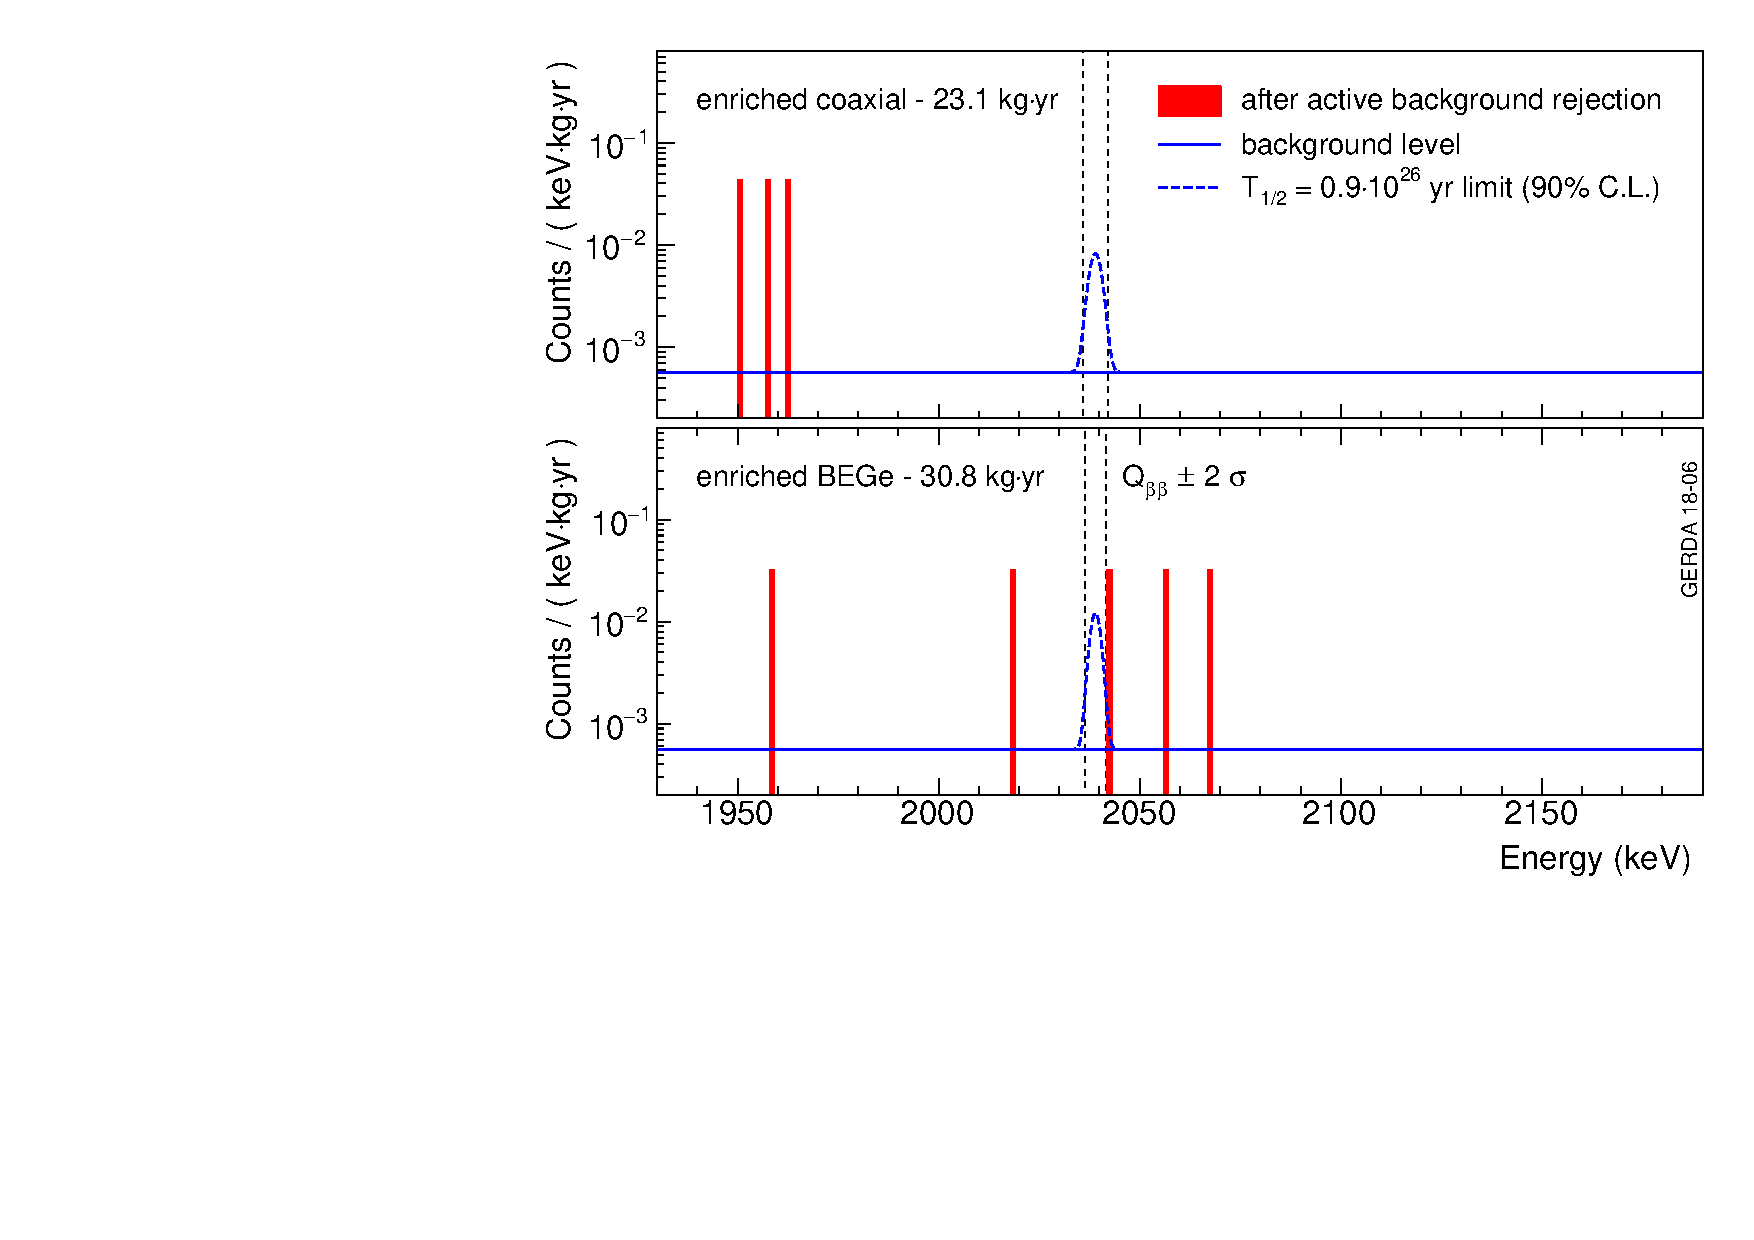
\includegraphics[width=0.8\linewidth]{plots/0nbb-results/roi-unblinded.pdf}
  \caption{%
    Events that survive all cuts in the background window. \fillme{to be updated}
  }\label{fig:gerda:roi}
\end{figure}

% vim: tw=90

  %!TEX root = ../main.tex

\chapter{The background before analysis cuts}\label{chap:bkg:raw:ph2}

As already mentioned, a precise knowledge of background intensity and distribution is
essential to searches of faint signals. One main assumption of the \onbb-decay signal
analysis is the distribution of background events in the analysis window around \qbb\
being uniform, except for the known \Tl\ and \Bil\ \g\ lines. The primary role of the
background model is to verify this assumption by exploiting data outside this energy
region or filtered with a different event selection. The background model is also
complementary to assay measurements in determining the location of the most dangerous
background sources and learn how to improve experimental design and material selection in
similar future projects. Lastly, a good background model allows to isolate \nnbb-decay
events, estimate the half-life of the process and study their distribution as a source of
potential new-physics effects (see \cref{chap:theory}).
\newpar
A first background model has been built for the \gerda\ \phaseone\ data and published
in~\cite{Agostini2013a}. Later, a new and advanced model has been constructed to describe
the first 60~\kgyr\ of \phasetwo\ data before the LAr veto and PSD cuts, which has been
published in~\cite{Agostini2019b} and is described in detail in this chapter. In
\cref{sec:bkg:raw:ph2:data} the selected data is presented and characterized, while the
procedure to compute the theoretical expectations used in the statistical analysis is
outlined in \cref{sec:bkg:raw:ph2:pdfs} (the topic is addressed in more detail in
\cref{apdx:magepdfs}). The prior knowledge about the presence of contaminants in the
\gerda\ setup that contribute to the germanium background spectrum is summarized in
\cref{sec:bkg:raw:ph2:priors}. The statistical framework and the analysis strategy is
presented in \cref{sec:bkg:raw:ph2:stat}. As it will be shown, the high-statistic \kvn,
\kvz\ and \a\ event data samples deserve dedicated studies and are thus treated
separately. These potassium and \a\ event analyses are presented in
\cref{sec:bkg:raw:ph2:kmodel} and \cref{sec:bkg:raw:ph2:amodel} respectively. Finally, the
results of the background decomposition in the full energy range of data from the first
part of \phasetwo\ are given in \cref{sec:bkg:raw:ph2:gmodel} and discussed in
\cref{sec:bkg:raw:ph2:discussion}. To complete the survey of background contributions to
the complete \gerdatwo\ energy spectrum before analysis cuts, the background model of data
from the second part of \phasetwo\ (\phasetwop) is presented in \cref{sec:bkg:raw:ph2p}.

\section{Analysis data sets}%
\label{sec:bkg:raw:ph2:data}

\begin{figure}
  \centering
  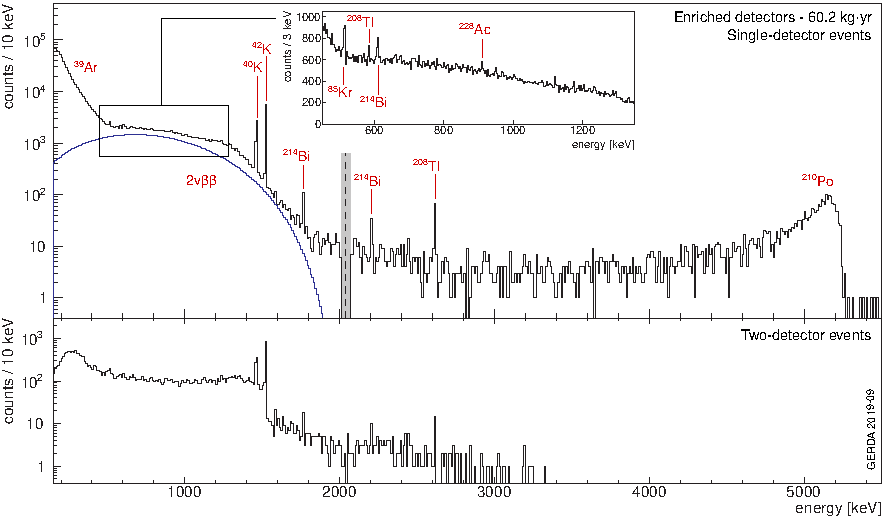
\includegraphics[width=0.9\linewidth]{plots/bkg/raw/ph2/dataGe-desc.pdf}
  \caption{%
    Summed energy spectra of single-detector events (\enrBEGeII\ and \enrCoaxII, top
    panel) and two-detector events (\enrGeII, bottom panel) collected in \gerda\
    \phasetwo.  The prominent features due to detector intrinsic \nnbb\ events, \kvz,
    \Arl\ and \Kr\ in the LAr, \kvn, the \Thh\ and \Uh\ decay chains are highlighted. The
    window blinded for the \onbb\ analysis is marked in grey.
  }\label{fig:bkg:raw:ph2:datasets}
\end{figure}

\begin{table}
  \centering
  \caption{%
    Properties of the data sets considered in this analysis. Further details about the
    \gerda\ detectors can be found in past publications~\cite{Agostini2013a,
    Agostini2018a}.  Note that the \bege\ exposure of 31.1~\kgyr\ is higher than the one
    reported in~\cite{Agostini2019a} because additional data for which PSD methods are not
    applicable is here included.
  }\label{tab:bkg:raw:ph2:datasets}
  \small
  \begin{tabular}{lccccc}
  \toprule
  \mr{2}{data set} & \mr{2}{composition}     & total Ge           & active \gesix\   & total Ge           & active \gesix\     \\
                   &                         & mass (kg)          & mass (kg)        & exposure (\kgyr)   & exposure (\kgyr)   \\
  \midrule
  \enrBEGeIIp\     & 29 \bege\footnotemark{} & $19.362 \pm 0.005$ & $17.17 \pm 0.32$ & $22.181 \pm 0.006$ & $17.31  \pm 0.32$  \\
  \enrSCoaxIIp\    & 6 \scoax\               & $11.827 \pm 0.002$ & $10.38 \pm 0.42$ & $13.179 \pm 0.003$ & $10.00  \pm 0.42$  \\
  \enrICoaxIIp\    & 4 \icoax\               & $ 7.802 \pm 0.002$ & $ 7.23 \pm 0.03$ & $ 8.775 \pm 0.002$ & $ 7.13  \pm 0.03$  \\
  \enrGeIIp\       & all enriched            & $38.991 \pm 0.006$ & $34.78 \pm 0.53$ & $44.135 \pm 0.007$ & $34.44  \pm 0.53$  \\
  \bottomrule
\end{tabular}

% vim: nowrap

\end{table}%
\footnotetext{%
  The \bege\ detector \GD{02D} is the only detector that does not fully
  deplete~\cite{Agostini2018a}. Hence, events triggered by this detector are
  not considered in either data set and it is omitted from the mass
  computation.
}

As already mentioned, the background model before cuts has been developed using data from
the first part of \phasetwo, namely, for data acquired starting from December 2015 to
March 2018. Single-detector (or multiplicity-one, abbreviated \Mone) events and
two-detector (multiplicity-two, abbreviated \Mtwo) events are considered for this
analysis. Events from the semi-coaxial detectors with natural isotope composition, located in
the central detector string, are not used in this analysis due to large uncertainties on
their \nplus\ contact thickness and detection efficiency. The \Mone\ events are split in
two data sets based on the two enriched detector geometries which we call \enrBEGeII\ and
\enrCoaxII\ in the following.  The \Mtwo\ data form a third data set which is named
\enrGeII. The energy we associate to an \Mtwo\ event is the sum of the energies
reconstructed in the two detectors. The data sets, their exposure and respective detector
mass are listed in \cref{tab:bkg:raw:ph2:datasets}.
\newpar
The event energy distribution of the three data sets is displayed in
\cref{fig:bkg:raw:ph2:datasets}: the sum spectrum of \enrBEGeII\ and \enrCoaxII\ in the
top panel and \enrGeII\ in the bottom panel. For the single-detector data, in the top
panel, the following features are most noticeable: the \b\ decay of \Arl\ dominates the
spectrum up to 565~keV while between 600 and 1500~keV the most prominent component is the
continuous spectrum of \nnbb\ decay of \gesix. Two \g\ lines at 1461 and 1525~keV can be
attributed to \kvn\ and \kvz; further visible \g\ lines belonging to \Kr, \Tl, \Bih\ and
\Ac\ are indicated in the figure. The highest energies displayed are dominated by a
peak-like structure emerging at 5.3~MeV with a pronounced low energy tail. This is a
typical spectral feature of \a\ particles and can, here, be attributed to \Po\ decay on
the thin detector \pplus\ surfaces~\cite{Agostini2013a}.  Events above the \Po\ peak
belong to \a\ decays emerging from the \Ra\ sub-chain on the detector \pplus\ surfaces.
All these components contribute also to \enrGeII\ except for \Arl, \nnbb\ and high energy
\a-components. This is due to the short range of \a\ (tens of \mum) and \b\
particles (typically smaller than 1.5~cm) in LAr and germanium with respect to the
distance between detectors which is of the order of several cm.

\section{Monte Carlo simulations and probability density functions}%
\label{sec:bkg:raw:ph2:pdfs}

The probability density functions (pdfs) used to model contributions to the energy spectra
are obtained from Monte Carlo simulations. The latter are performed using the \mage\
simulation framework~\cite{Boswell2011}, based on
\geant~\texttt{v10.4}~\cite{Agostinelli2002, Allison2006, Allison2016}.  \mage\ contains a
software implementation of the \gerdatwo\ detectors as well as the assembly and all other
surrounding hardware components. A visualization of this implementation is presented in
\cref{fig:setup:magevolumes}. Detector intrinsic \nnbb\ decays of \gesix\ and background
events originating from radioactive contaminations in and around the detector assembly are
simulated. The energy spectrum of the two electrons emitted in the \nnbb\ decay is
sampled according to the distribution given in~\cite{Tretyak1995} and implemented in
\decayzero~\cite{Ponkratenko2000}. The pdfs are obtained from the Monte Carlo simulations,
taking into account the finite energy resolution and individual exposure acquired with
each detector during the considered data taking periods. Special care is taken not to
statistically bias the pdfs by assuring that each simulated decay is taken into account
only once in the production of a pdf. For more details see \cref{apdx:magepdfs}. The
germanium detector active volume model is also applied to the simulations during this
post-processing step. A simplified step-like function that defines the charge-collection
efficiency (CCE) value depending on the depth from the detector surface is used to produce
the pdfs for the analysis of \phasetwo\ data before the upgrade. The CCE is set to a null
value through all the transition region between the surface and the full charge-collection
efficiency region. From the full charge-collection depth (FCCD) and below the CCE is set
equal to unity. The recommended FCCD values obtained from dedicated characterization data
(the same used in the \onbb\ detection efficiency calculation) are documented and
discussed in \cref{apdx:gedetav}. The pdfs for the background model of \gerdatwo\ data
before cuts are displayed in
\cref{fig:bkg:raw:ph2:pdfs:gmodel,fig:bkg:raw:ph2:pdfs:amodel,fig:bkg:raw:ph2:pdfs:kmodel:K40,fig:bkg:raw:ph2:pdfs:kmodel:K42}
and will be presented in more detail in the following.

\section{Background expectations}%
\label{sec:bkg:raw:ph2:priors}

\begin{figure}
  \centering
  \subfloat[\label{fig:bkg:raw:ph2:pdfs:gmodel:Th}%
    \Bil\ and \Tl\ (\Thh\ chain) contaminations far from (fiber shroud) and close to
    (mini-shrouds) the detectors.
  ]{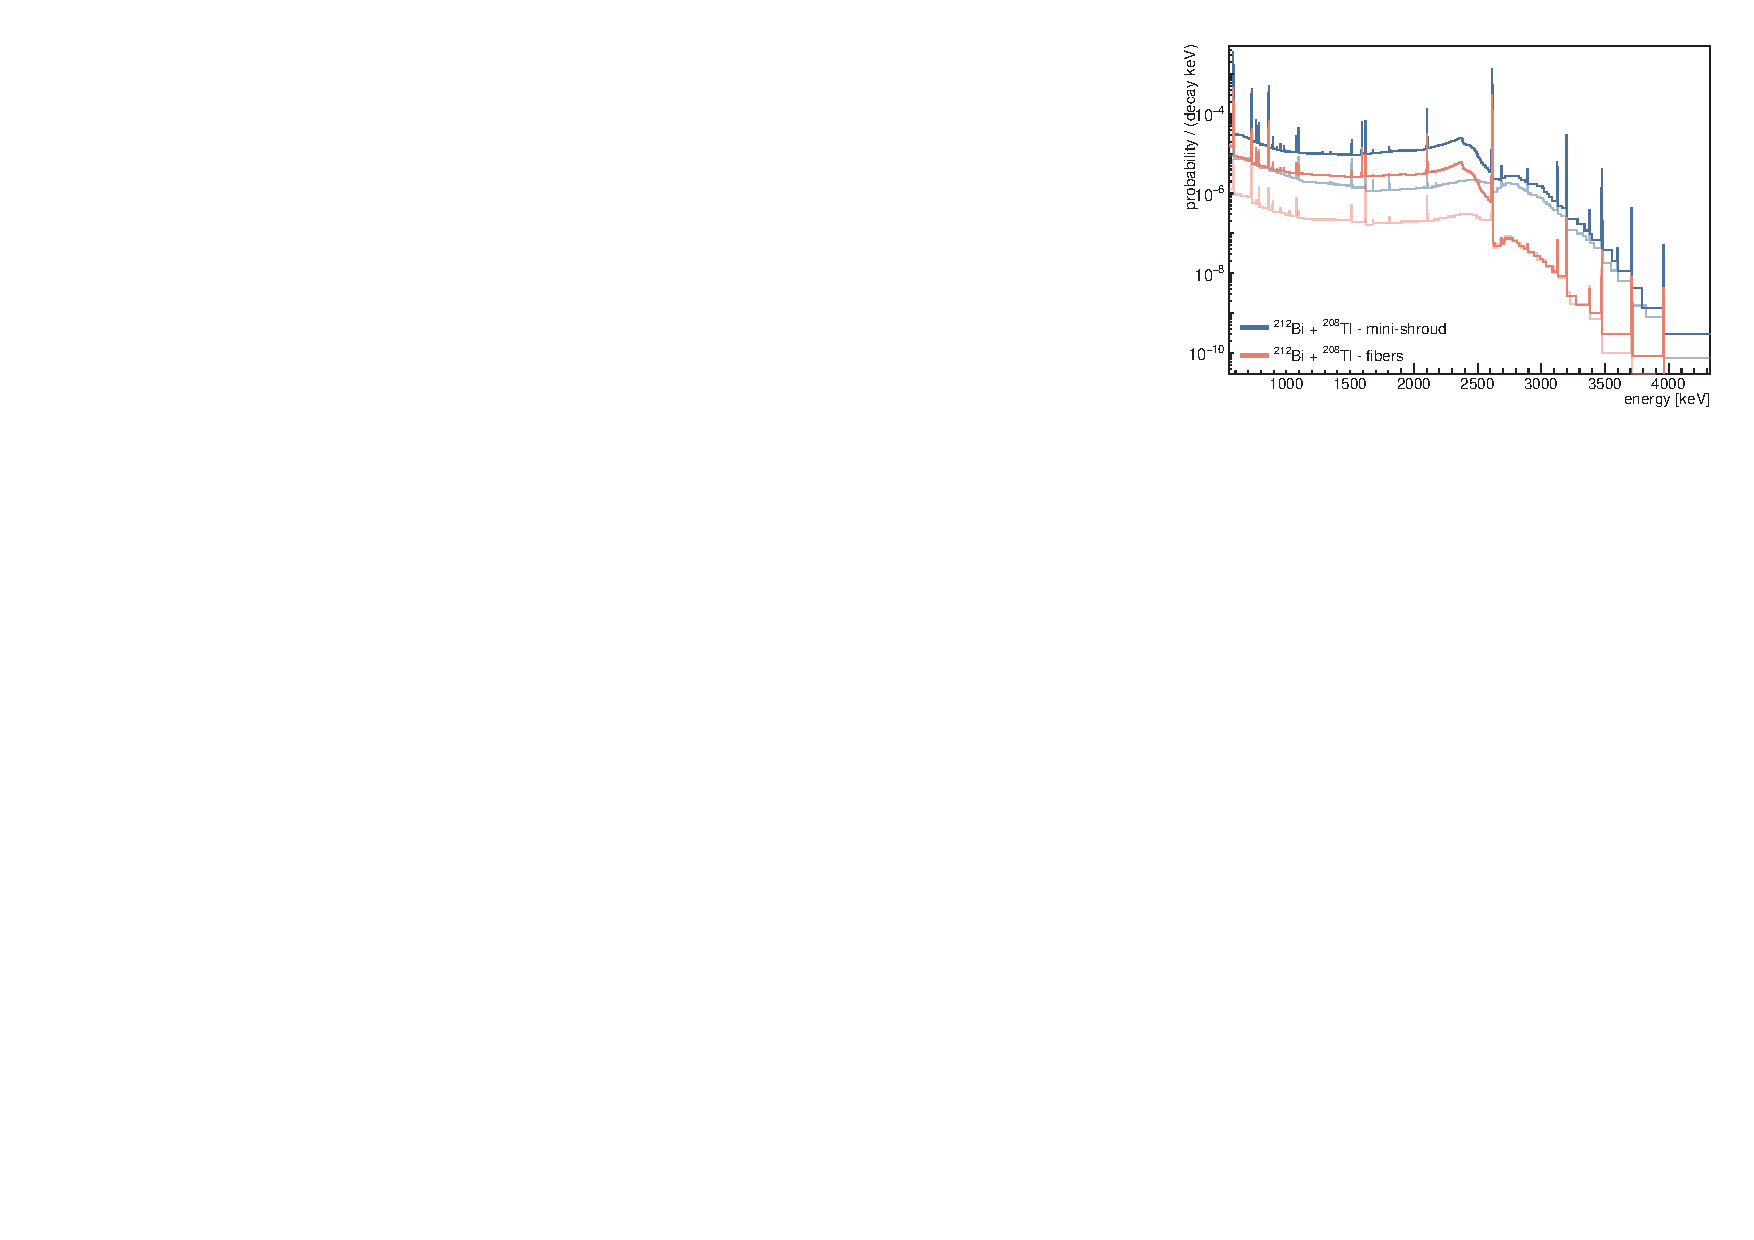
\includegraphics[width=0.48\textwidth]{plots/bkg/raw/ph2/pdfs/gmodel-pdfs-Th.pdf}}
  \hfill
  \subfloat[\label{fig:bkg:raw:ph2:pdfs:gmodel:U}%
    \Bih\ and \Pbh\ (\Uh\ chain) contaminations far from (fiber shroud) and close to
    (mini-shrouds) the detectors.
    ]{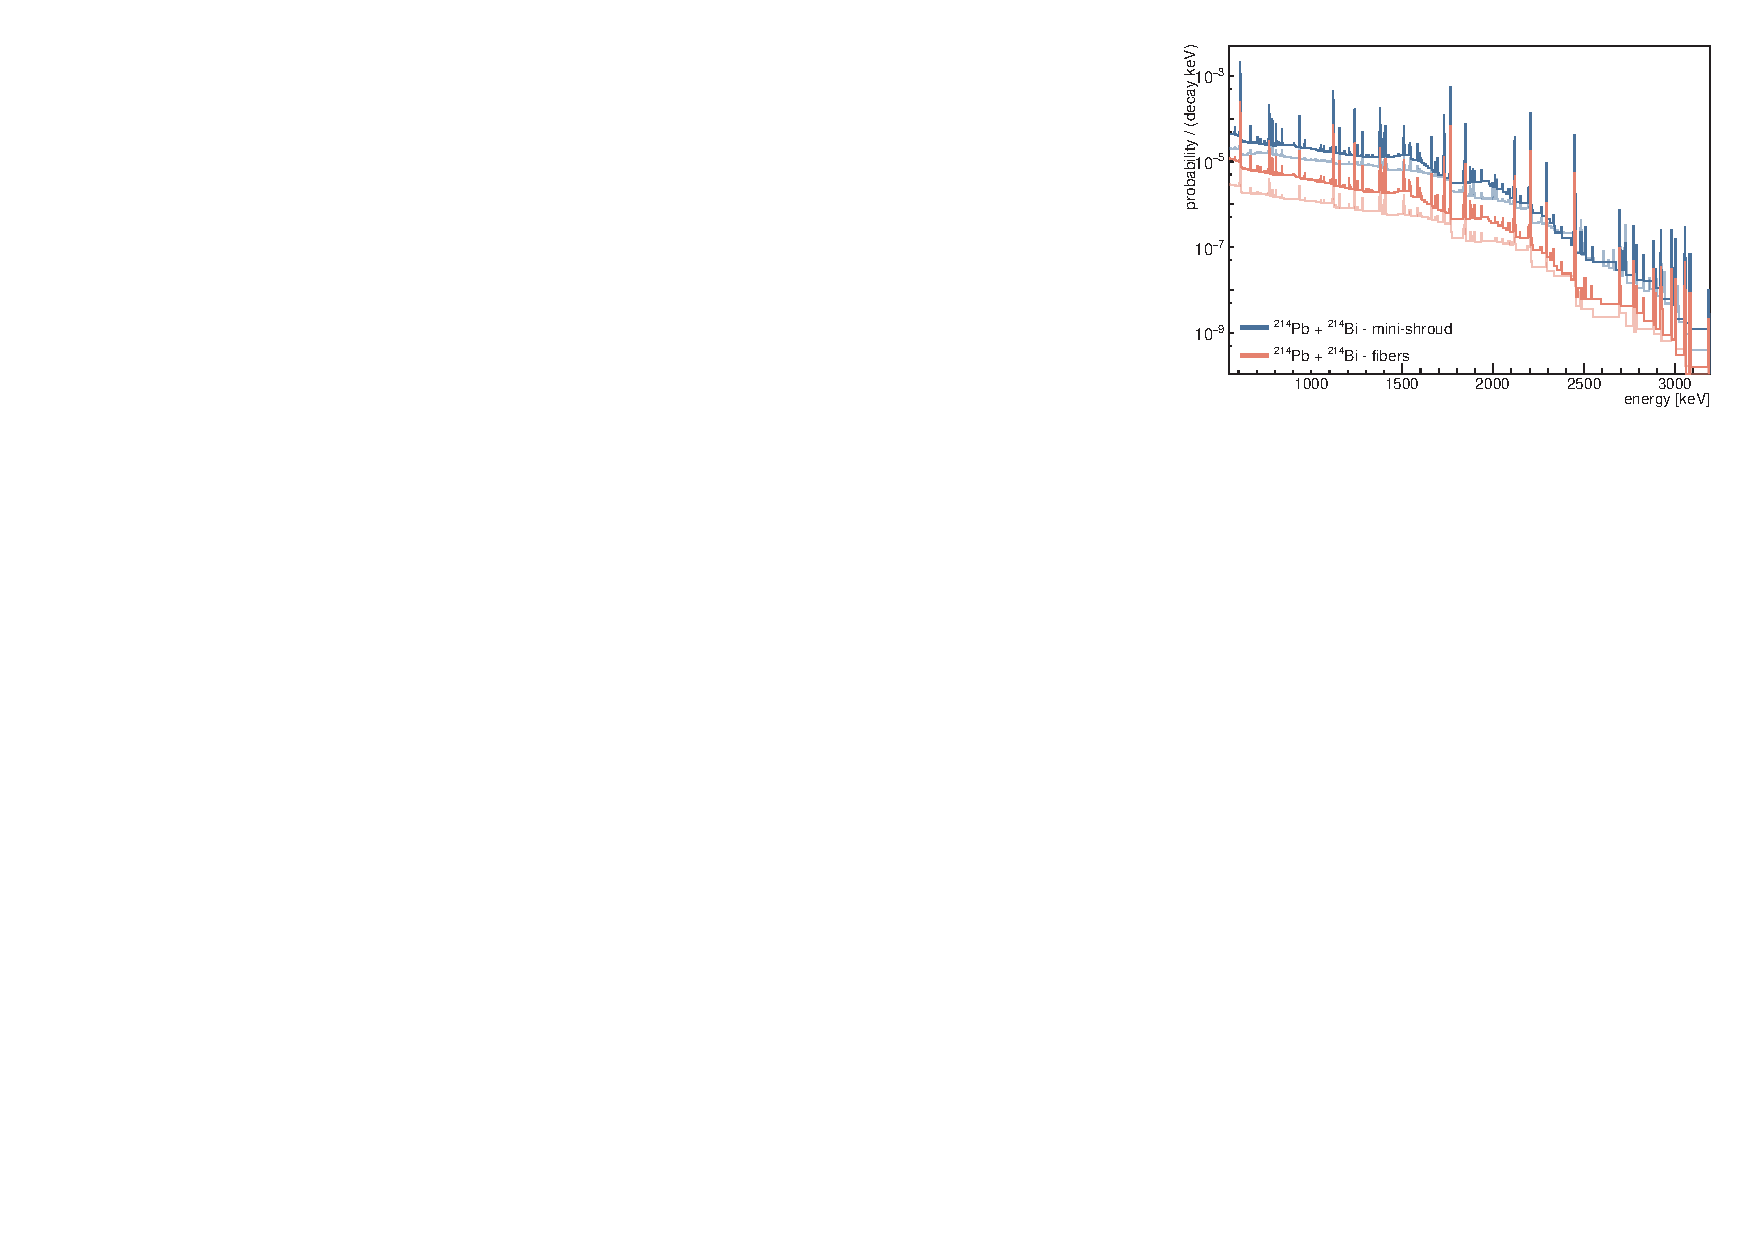
\includegraphics[width=0.48\textwidth]{plots/bkg/raw/ph2/pdfs/gmodel-pdfs-U.pdf}}

  \subfloat[\label{fig:bkg:raw:ph2:pdfs:gmodel:K40}%
    \kvn\ contamination close to the detectors (mini-shrouds), at a higher radial distance
    (fiber shroud) and higher vertical distance (copper shrouds).
  ]{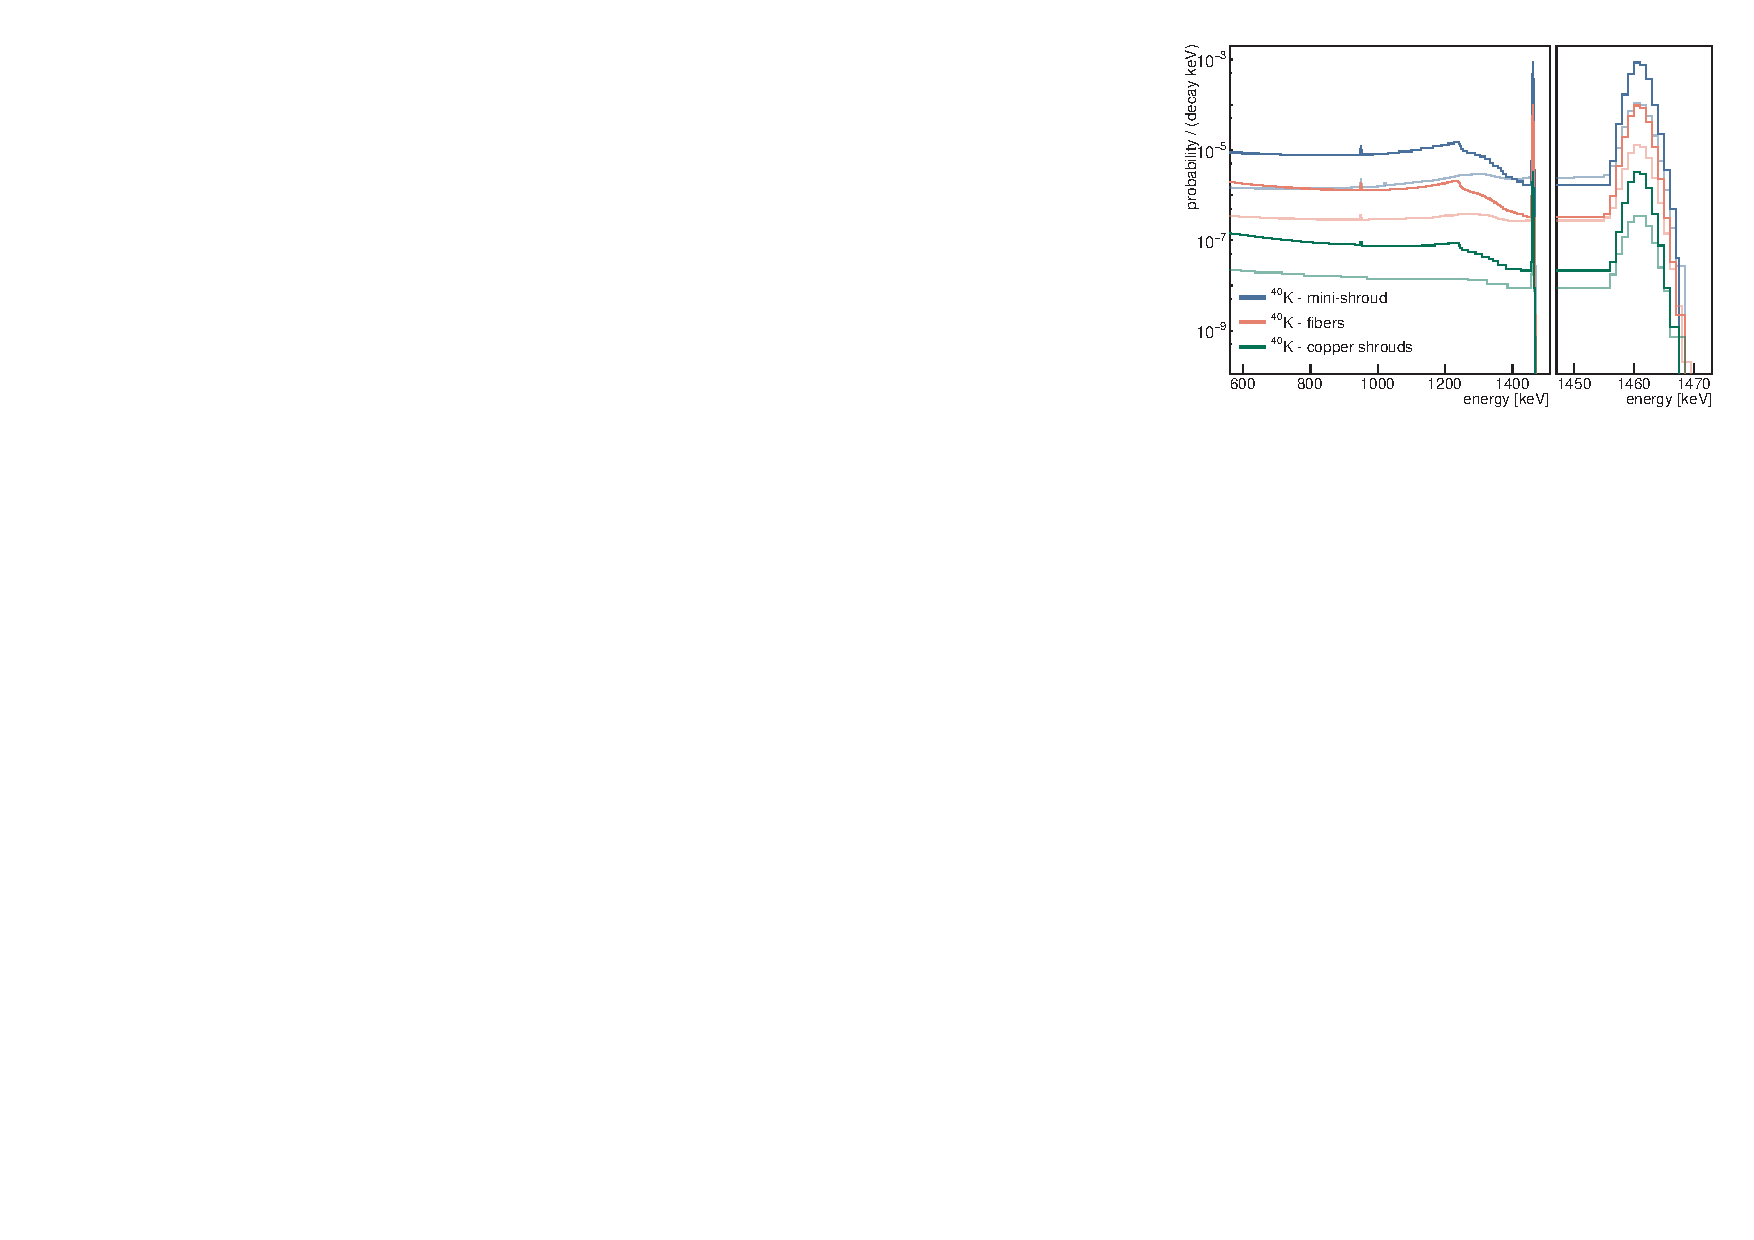
\includegraphics[width=0.48\textwidth]{plots/bkg/raw/ph2/pdfs/gmodel-pdfs-K40.pdf}}
  \hfill
  \subfloat[\label{fig:bkg:raw:ph2:pdfs:gmodel:K42}%
    \kvz\ contamination in different locations inside the LAr.
  ]{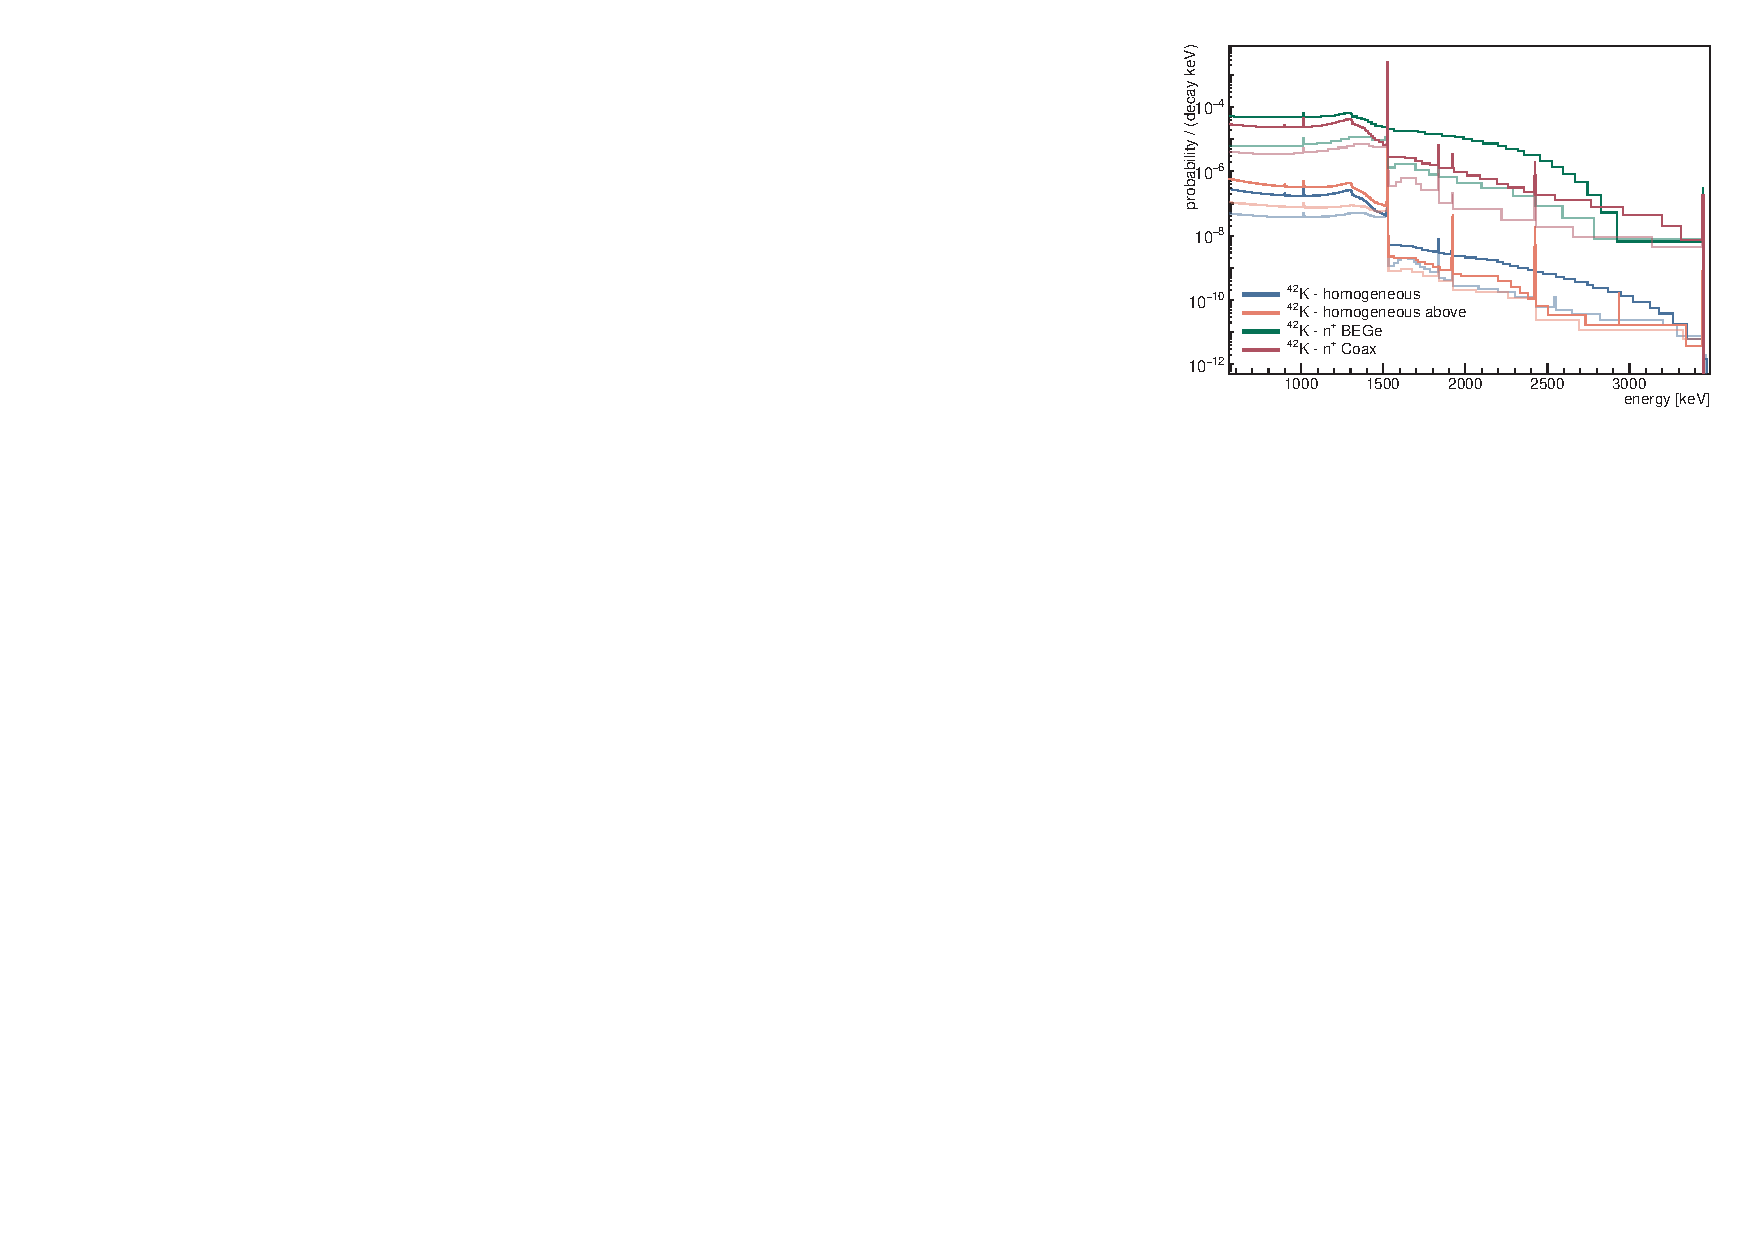
\includegraphics[width=0.48\textwidth]{plots/bkg/raw/ph2/pdfs/gmodel-pdfs-K42.pdf}} \\

  \subfloat[\label{fig:bkg:raw:ph2:pdfs:gmodel:other}%
  \Pa\ and \Ac\ contaminations in the close vicinity of the detectors (mini-shrouds).
  ]{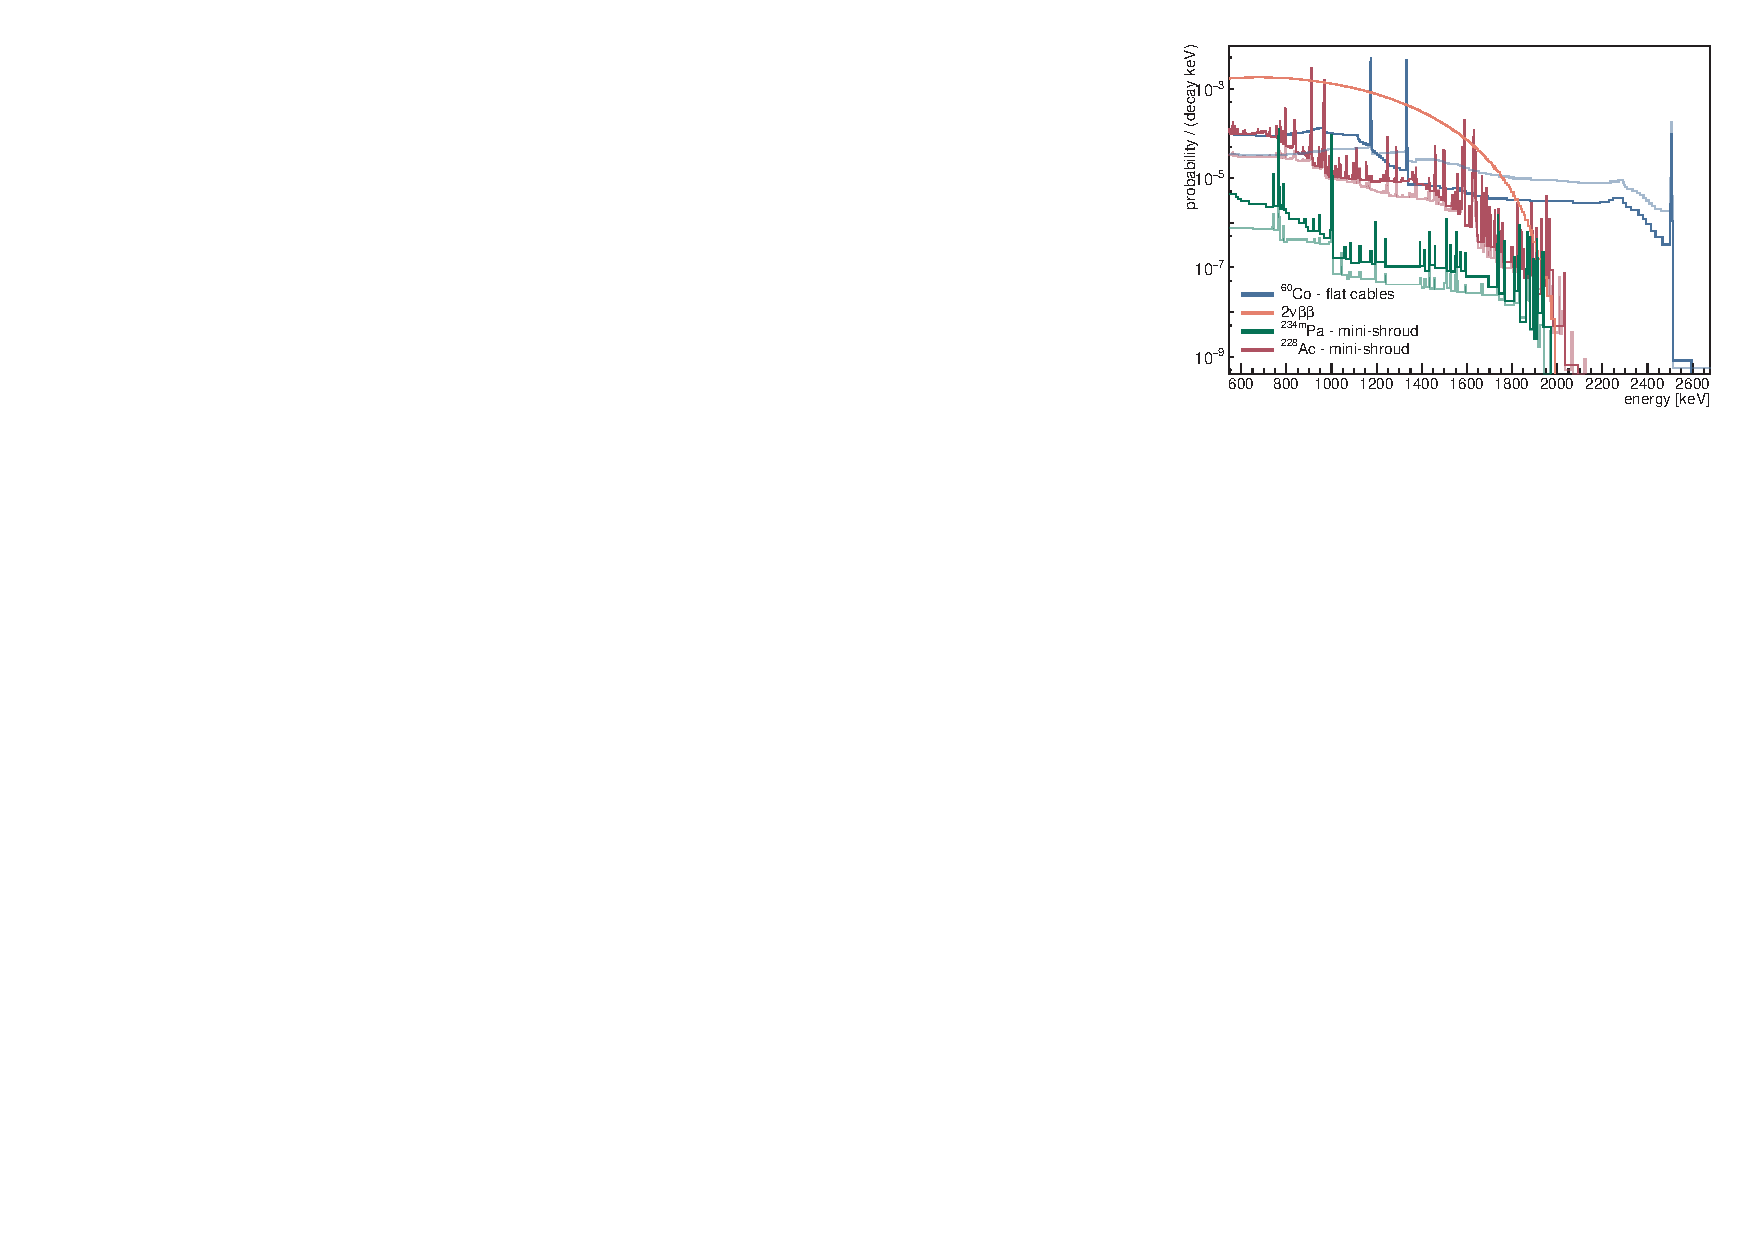
\includegraphics[width=0.48\textwidth]{plots/bkg/raw/ph2/pdfs/gmodel-pdfs-misc.pdf}}
  \hfill
  \subfloat[\label{fig:bkg:raw:ph2:pdfs:gmodel:other2}%
    \Co\ contamination in the signal and high-voltage cables and detector intrinsic
    \gesix\ \nnbb\ decay.
  ]{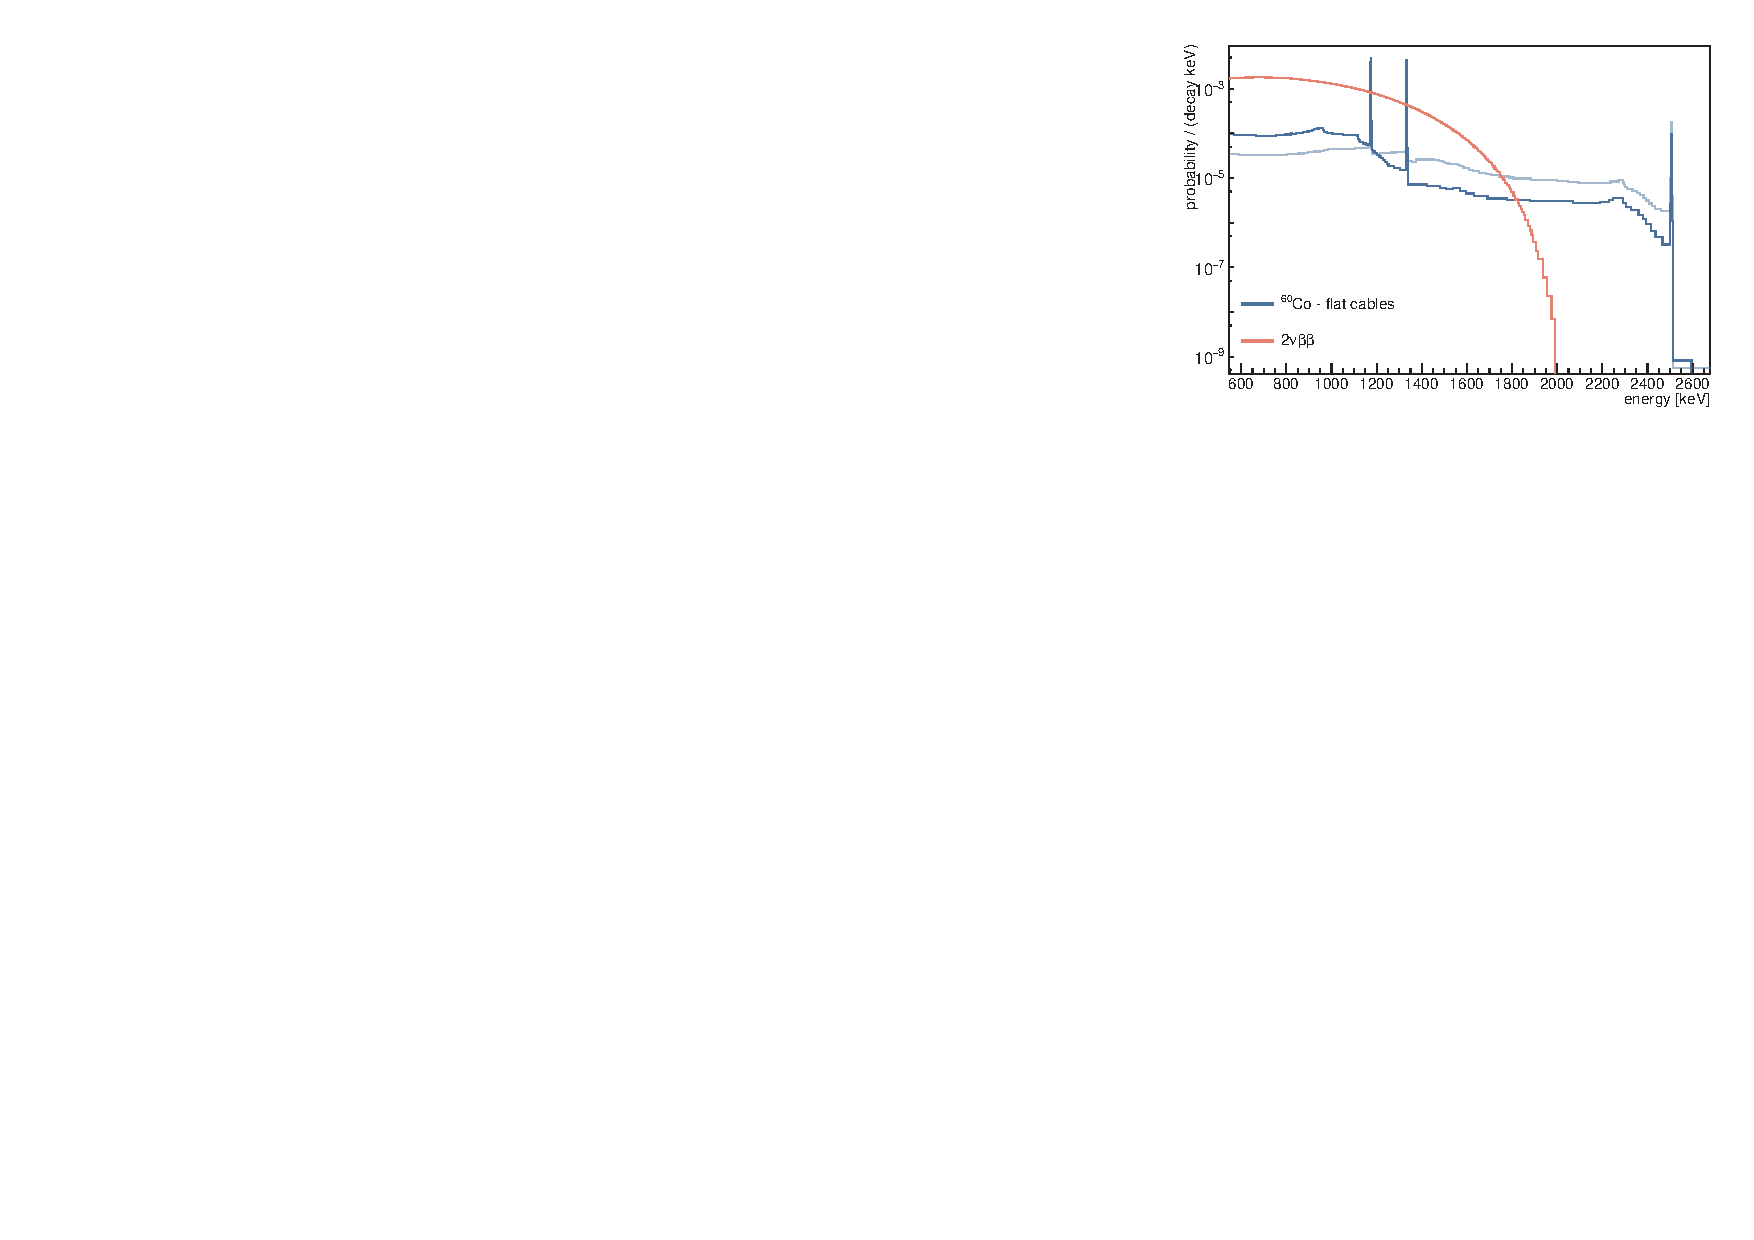
\includegraphics[width=0.48\textwidth]{plots/bkg/raw/ph2/pdfs/gmodel-pdfs-misc2.pdf}}

  \caption{%
    The pdfs for the \m{M1-AllEnr} ($\enrBEGeII + \enrCoaxII$) (in fully opaque colors) and
    the \enrGeII\ (in shaded colors) data sets in the full energy domain and relative to
    different background sources. Bayesian blocks are used to visualize histograms (see
    \cref{apdx:bayesblocks} for details). All pdfs are normalized to the number of
    simulated events.
  }\label{fig:bkg:raw:ph2:pdfs:gmodel}
\end{figure}

The structural components of the setup have been screened for their radio-purity before
deployment. Two measurement methods were used depending on the screened isotope: \g-ray
spectroscopy (Ge-\g) with high-purity germanium (in four underground laboratories, for
details see reference~\cite{Ackermann2012}) and mass spectrometry with Inductively Coupled
Plasma Mass Spectrometers (ICP-MS)~\cite{Vacri2015}. Especially materials close to the
detectors have been screened for radioactive contaminations originating from the \Uh\ and
\Thh\ decay chains, \kvn\ and \Co. For measured activities and upper limits see
\cref{apdx:assay} and sec.~5 in~\cite{Agostini2018a}. All possible background sources
taken into consideration in this analysis are described in detail below.

\blocktitle{\Thh\ \\ \Uh}
The only isotopes simulated are \Pa, \Pbh\ and \Bih\ from the \Uh\ decay chain and \Ac,
\Bil\ and \Tl\ from the \Thh\ decay chain. The following groups of isotopes are assumed to
be in secular equilibrium:
\[
  ^{238}\text{U}  \succ ^{234\text{m}}\text{Pa}               \;\; \| \;\;
  ^{226}\text{Ra} \succ ^{214}\text{Pb} \succ ^{214}\text{Bi} \;\; \| \;\;
  ^{228}\text{Ra} \succ ^{228}\text{Ac}                       \;\; \| \;\;
  ^{228}\text{Th} \succ ^{212}\text{Bi} \succ ^{208}\text{Tl} \;.
\]
Their decay products consist of \g\  or \b\ particles with an energy higher than 520~keV
(\cref{fig:bkg:raw:ph2:pdfs:gmodel:U,fig:bkg:raw:ph2:pdfs:gmodel:Th,fig:bkg:raw:ph2:pdfs:gmodel:other}).
Less energetic particles from the remaining constituents in the chain do not enter the
energy window which is considered in the presented analysis.  The \a\ emitters from the
decay chains contaminating the thin \pplus\ electrodes are described in a separate
paragraph below.

\blocktitle{\Co}
A significant fraction of components in the \gerda\ setup is made of
copper~\cite{Agostini2018a}, which can be produced with high radio-purity but is
potentially activated by cosmic rays and contaminated by the long-lived isotope \Co\
(\cref{fig:bkg:raw:ph2:pdfs:gmodel:other}). The latter decays with a half-life of
5.2711(8)~yr; from material screening it is also expected to be found in some of the
detector high-voltage flexible flat cables.

\blocktitle{\kvn}
This isotope is found in all screened materials.  Construction materials were not
optimized for ultra-low \kvn\ content because the Q-value of its decay is well below \qbb\
and hence does not contribute to the background in the ROI. The \kvn\ decay spectrum
exhibits a \g\ line at 1460.822(6)~keV (see \cref{fig:bkg:raw:ph2:pdfs:gmodel:K40}) with
an accumulated statistics on the order of 100~cts/detector. In
\cref{fig:bkg:raw:ph2:pdfs:kmodel:K40} the expected counts per detector channel for \kvn\
simulated in different locations are shown. Using the ratio of events detected in
different detectors, information about the spatial distribution of \kvn\ can be extracted.
This spatial information is used to resolve degeneracies of \kvn\ in the energy spectra
(for details see \cref{sec:bkg:raw:ph2:kmodel}).

\blocktitle{\kvz}
A cosmogenically-produced isotope in LAr is \Arh\ ($T_{1/2} = 32.9(11)$~yr) which decays
to \kvz. The distribution of \kvz\ inside the LAr is likely to be inhomogeneous due to
drift of the ionized decay products induced by the electric field (generated by
high-voltage cables and detectors) and convection~\cite{Pelczar2016}. \kvz\ decays to
$^{42}$Ca via \b\ decay with a half-life of 12.355(7)~h and a Q-value of 3525.22(18)~keV,
well above \qbb\ (see \cref{fig:bkg:raw:ph2:pdfs:gmodel:K42}). For the \b\ particle to be
detected the decay needs to happen within a distance of a few centimeters\footnote{%
  The path length of \kvz\ \b\ particles in LAr is less than 1.6~cm, but bremsstrahlung
  photons from the interaction with LAr can travel as far as $\sim$10~cm.
} to the detector surface. As the detectors are
in direct contact with the LAr, the \b\ component of \kvz\ potentially gives one of the
most significant contributions to the background in the ROI. Therefore, we separate decays
originating inside and outside the mini-shrouds in the following analysis. The full-range
fit has little sensitivity to any potassium inhomogeneity outside the mini-shrouds. \kvz\
is hence assumed to be distributed homogeneously in this region. Based on detector-wise
observations, however, a surplus of \kvz\ above the detector array in the vicinity of the
front-end electronics is deduced (see \cref{sec:bkg:raw:ph2:kmodel}). Inside the
mini-shrouds the \b\ spectrum becomes potentially important.  Some scenarios are possible:
the closer \kvz\ decays to the detector surface, namely to the \nplus\ and \pplus\
contacts, the more \b\ particles enter the germanium. A fraction of events around \qbb\
coming from \kvz\ is potentially due to \g\ particles with higher energy and sub-percent
level branching ratio or simultaneous energy deposition of multiple \g\ particles. This
\g\ component could become important for large quantities of \kvz\ not located directly on
the detector surfaces with the \b\ particle being absorbed in the LAr. As for \kvn\ also
the \g\ line at 1525~keV of \kvz\ contains valuable information about the spatial decay
distribution of this isotope. In contrast to \kvn\ no additional information, e.g.~from
radio-purity screening measurements, is available. For more detailed information about
\kvn\ and \kvz\ see \cref{sec:bkg:raw:ph2:kmodel}.

\blocktitle{\a\ emitters}
The lithium-diffused \nplus\ detector surfaces act as a barrier for \a\ particles. The
latter can only penetrate the very thin boron-implanted \pplus-contact or the contact
separating groove. \a\ particles have to be emitted directly at the surface or from a thin
adjacent layer of LAr. Since \a\ particles have to cross the $\sim 0.5$~\mum\ thick
\pplus\ dead layer and therefore only part of their initial energy is deposited in the
active volume, this background component leads to peaks with characteristic low-energy
tails in the HPGe energy spectra (see \cref{fig:bkg:raw:ph2:pdfs:amodel}). Some \a\
events, presumably originating from the detector groove, are reconstructed with degraded
energy and lead to an additional, continuous spectral component. We find mainly \Po\ but
also traces of isotopes from the \Ra\ decay chain.

\blocktitle{detector \\ bulk \\ impurities}
Cosmogenically produced long-lived isotopes can also be found in
germanium~\cite{Meierhofer2009, Meierhofer2010, Meierhofer2012}. In particular, $^{68}$Ge
and \Co\ can occur as detector intrinsic impurities with half-lives of 270.93(13)~d and
5.2711(8)~yr.  The \bege\ detectors were kept underground during major parts of the
fabrication and characterization operations. Periods when these detectors were above
ground have been tracked in a database~\cite{Agostini2015e}.  Thus, for the well-monitored
BEGe detectors we expect impurities of 5~nuclei/kg of $^{68}$Ge and 21~nuclei/kg of \Co\
as of September 2014~\cite{Agostini2015e}. Extrapolating the expected impurities to the
whole \phasetwo\ data taking period we expect on average 0.03~cts/day from $^{68}$Ge and
0.1~cts/day due to \Co. From background modeling in Phase I~\cite{Agostini2013a} the
contribution for the coaxial detectors formerly used in the Heidelberg-Moscow
(\hdm)~\cite{Klapdor2001} and \igex~\cite{Aalseth2002} experiments is expected to be even
smaller due to their long storage underground. Simulating the expected detector bulk
impurities we find background contributions around \qbb\ of less than $10^{-4}$~\ctsper\
in both cases. Hence, we conclude that $^{68}$Ge as well as \Co\ can be neglected in the
following analysis. Potential bulk contaminations with \Uh\ and \Thh\ were studied in
reference~\cite{Agostini2016a}. Only upper limits were found, establishing germanium
crystals as material of outstanding radio-purity.  Hence, only the decay of \gesix\ via
\nnbb\ as detector intrinsic background component is considered while all other intrinsic
impurities are considered to be negligible.

\blocktitle{other \\ sources}
Prompt cosmic muon induced background events are efficiently vetoed by the identification
of \v{C}erenkov light emitted by muons when they pass the water tank~\cite{Agostini2013a}.
The expected background indices, due to the direct muon and neutron fluxes at the LNGS underground
laboratory, have been estimated to be of the order $3 \cdot
10^{-5}$~\ctsper~\cite{Freund2014} and $10^{-5}$~\ctsper~\cite{Meierhofer2012} in earlier
works, respectively.  Background contributions coming from delayed decays of $^{77}$Ge and
$^{77\text{m}}$Ge, also induced by cosmic muons, are estimated to be $0.21 \pm
0.01$~nuclei/(kg$\cdot$yr)~\cite{Wiesinger2018} corresponding to a background index prior to the active
background suppression techniques of about $10^{-5}$~\ctsper. Also, the water tank and LAr
cryostat contaminations are expected to contribute to the \gerda\ background index with less than
$10^{-4}$~\ctsper~\cite{Ackermann2012, Barabanov2009}. All above mentioned contributions
are considered negligible in this work. Other potential sources of background from
interactions of \gesix~\cite{Meierhofer2012, Vanhoefen2018} and $^{206}$Pb~\cite{Mei2007}
with neutrons and $^{56}$Co for which no evidence was found are not taken into
consideration. The cosmogenically-produced isotope \Arl\ and the anthropogenic isotope
\Kr~\cite{Winger2005}, which are dissolved in LAr, emit particles which are dominantly
less energetic than the energy window which is considered in the presented analysis.

\section{Statistical analysis}%
\label{sec:bkg:raw:ph2:stat}

The multivariate statistical analysis, which is used to model and disentangle the
background in its components, runs on the three binned data sets \enrBEGeII, \enrCoaxII\
and \enrGeII. The single-detector data sets \enrBEGeII\ and \enrCoaxII\ contain the
reconstructed energy of all \Mone\ events whereas for the two-detector events the sum of
the two reconstructed energies is put in the \enrGeII\ data set. Moreover, the count rate
per detector is used for the two potassium \g\ lines.  The spatial event distribution is a
collection of the number of events per detector for \Mone\ events and expressed in a
matrix of pairs of detectors for all \Mtwo\ events.

\blocktitle{likelihood}
\sloppy Assuming that the number of events in each bin follows the Poisson probability
distribution $\operatorname{P}(n;\nu)$, where $\nu$ is the expected mean and $n$ is the
experimentally measured number of counts, the likelihood function for a binned data set
reads $\prod_{i=1}^{N_\text{bins}} \operatorname{P}(n_i;\nu_i)$. Here $\nu_i =
\sum_{k=1}^{N_\text{com}} \nu_i^{(k)}$ is the expected number of events in the $i$-th bin,
calculated as the sum of the contributions from each background component $k$;
$\nu_i(\lambda_1, \ldots, \lambda_{N_\text{com}})$ is a function of the parameters of
interests $\lambda_j$ (isotope activities, \nnbb\ half-life, etc.). The complete
likelihood function adopted for the present analysis combines the three data sets
\enrBEGeII, \enrCoaxII\ and \enrGeII:
\begin{equation}\label{eq:bkg:raw:ph2:likelihood}
  \mathcal{L}(\lambda_1, \ldots, \lambda_m \,|\, \text{data}) =
    \prod_{d=1}^{N_\text{dat}}
    \prod_{i=1}^{N_\text{bins}}
    \operatorname{P}(n_{d,i};\nu_{d,i})\;.
\end{equation}

\blocktitle{statistical \\ inference}
The statistical inference is made within a Bayesian framework. Hence, to obtain posterior
probabilities for the free parameters of interest $\lambda_j$, the likelihood defined in
\cref{eq:bkg:raw:ph2:likelihood} is multiplied according to the Bayes theorem by a factor
modeling the prior knowledge of each background component as presented in
\cref{sec:bkg:raw:ph2:priors}. The computation is performed using a Markov Chain Monte
Carlo (MCMC) methods and is implemented using the BAT software package~\cite{Caldwell2008,
Beaujean2018}. Posterior probability distributions of any observable that is not a free
parameter of the likelihood function, like background index estimates, are obtained by
sampling the desired parameter from the MCMC. A \pvalue\ estimate is provided as a
goodness-of-fit measure by adopting the algorithm suggested in~\cite{Beaujean2011} for
Poisson-distributed data.  It has to be kept in mind that this \pvalue\ estimate, however,
is not as well suited for model comparison as is for instance a Bayes factor; e.g.~the
number of free parameters is not taken into account while a Bayes factor always penalizes
models that add extra complexity without being required by the data.

\blocktitle{analysis \\ window \\ and binning}
The fit range and data bins are chosen such as to exploit as much information from
spectral features as possible brought by data without introducing undesired bias. The
chosen fit range in energy space for the single-detector data sets (\enrBEGeII\ and
\enrCoaxII) starts from just above the end-point of the \Arl\ $\upbeta^-$-spectrum at
565~keV and ends just above the \Po\ peak at 5260~keV, where the event rate drops to
almost zero values. For the two-detector events (\enrGeII\ data set) the fit range starts
at 520~keV and extends up to 3500~keV. Possible additional components outside of this
range (e.g. \Arl) do neither add information to the background decomposition in the ROI
around \qbb\ nor to the analysis of \nnbb\ decay. Furthermore, at energies lower than
$\sim$100~keV the shape of the pdfs is dominated by uncertainties on the detector
transition layer model, which describes the charge-carrier collection at the interface
between the \nplus\ contact and the detector active volume. The exact nature of this
transition region is different for each detector and prone to systematic
uncertainties (see \cref{apdx:gedetav} for a detailed discussion).
\newpar
With an energy resolution which is typically 3--4~keV at \qbb\ (FWHM)~\cite{Agostini2018,
Agostini2019a} and better at lower energies, a fixed bin size of 1~keV was chosen for all
data sets. The only exceptions are the two \g\ lines from \kvn\ and \kvz\ each of which is
combined in a single bin from 1455~keV to 1465~keV and from 1520~keV to 1530~keV,
respectively. This is done in order to suppress any systematic uncertainties of the energy
calibration and resolution model that affect the position and shape of the \g\
lines~\cite{Agostini2019}.

\blocktitle{likelihood \\ factorization}
A feature of the selected data is that the likelihood in
\cref{eq:bkg:raw:ph2:likelihood} can be factorized in uncorrelated parts which can be
studied individually and in detail. In the following we shortly outline the parts of the
data which were studied in depth based on the approach of factorizing the likelihood into
uncorrelated parts. Finally, the results of these analyses are incorporated into a
full-range fit. This procedure is equivalent to a simultaneous analysis of all data but
increases the input knowledge for the fit and breaks down the computational complexity in
smaller steps.

\blocktitle{potassium \\ tracking \\ analysis}
As can be noted from \cref{fig:bkg:raw:ph2:pdfs:gmodel:K40} and
\cref{fig:bkg:raw:ph2:pdfs:gmodel:K42} the pdfs of \kvn\ and \kvz\ in energy from
different locations are prone to degeneracies and hence parameter correlation. Their most
prominent \g\ lines at 1461~and 1525~keV, respectively, contain information on the spatial
distribution while the two-detector events contain information about the angular
distribution of Compton scattered events. Their combination is beneficial in order to pin
down the potential location of the two potassium isotopes. In total the \Mone\ data
contains 4472~cts in $1461 \pm 4$~keV and 6718~cts in $1525 \pm 4$~keV while the \Mtwo\
events contain 554~cts in $1461 \pm 6$~keV and 865~cts in $1525 \pm 6$~keV, respectively.
An analysis of the number of events in the two potassium \g\ lines in each detector (and
detector pair) is used to exploit mainly top-down and rotational asymmetries in the \kvn\
and \kvz\ distributions. The events in the two energy windows are classified according to
the detectors in which an energy deposition was registered, so to exploit the available
information about the event location. In the following this classification procedure will
be referred to as `projection in detector space'. The treatment of the likelihood
in \cref{eq:bkg:raw:ph2:likelihood} is outlined in detail in
\cref{sec:bkg:raw:ph2:kmodel}.  The number of events in all other \g\ lines is too low in
order to adopt a useful detector-wise analysis. The spatial analysis of \kvn\ and \kvz\ is
incorporated in the full-range fit by directly employing the posterior parameter
distributions as prior information.\footnote{%
  By adopting this approach, a part of the data in the potassium \g\ lines region is
  analyzed twice: first in the potassium-tracking analysis and then in the full-range fit.
  Nevertheless, considering that the two analyses exploit different data features
  (i.e.~count rate per detector and total count rate per energy) and the overlap between
  the two data set is minimal, the overall effect is negligible.
}

\blocktitle{\a\ events background analysis}
The single-detector energy spectra above 3.5~MeV (the Q-value of \kvz\ \b\ decay) are
strongly dominated by \a\ events. They are not present in two-detector data due to the
short range of \a\ particles in LAr and germanium. Also, this component is not correlated
to other backgrounds considered here because it peaks at energies well above the highest
\g\ emission energies and \b\ decay Q-values. A careful study was carried out considering
various \pplus\ contact thickness and event rates to reproduce the \Po\ peak. In order to
reproduce \a\ events with degraded energy an empirical model is fit to the data. A linear
function with free slope and offset and a cut-off below the maximum of the \Po\ peak fits
the data well. The agreement of the \a\ background model with the data is demonstrated in
\cref{sec:bkg:raw:ph2:amodel} and \cref{apdx:timealpha}. Information from the detailed
analysis of the high-energy \a\ region is incorporated in the full-range fit using a
combined pdf that summarizes the \Po\ peak plus the \Ra\ decay chain and a linear floating
component for energy-degraded \a\ events.

\blocktitle{prior \\ distributions}
The following criteria are adopted to convert the prior information described in
\cref{sec:bkg:raw:ph2:priors} into prior probability distributions on the parameters of
interest to be used in Bayesian inference: if a measured value with uncertainty is
available for a background contamination then a Gaussian distribution with a corresponding
centroid and a $1\sigma$ width is adopted. In presence of a 90\% C.L.~upper limit,
instead, an exponential prior distribution is constructed with 90\% of its area covering
parameter values from 0 up to the given 90\% C.L.~upper limit (i.e. $p \sim e^{-\mu x}$).
A uniform prior distribution is assigned to components for which no measured value or
upper limit is available. Ranges for uniform priors are initially taken very wide, in
order to span a large portion of the allowed parameter space, then optimized to contain at
least 99\% of the posterior distribution. As mentioned before, in addition to the
information from screening measurements, prior distributions for \kvn\ and \kvz\ are
constructed considering the posterior inference from their spatial distribution. Moreover,
as \Bih\ is part of the \Ra\ decay chain, we constrain a \Bih\ component on the \pplus\
contact by a Gaussian prior extracted from the obtained \Ra\ activity based on the energy
estimator in the high-energy \a\ region.

\section{\texorpdfstring{\a\ events analysis}{alpha events analysis}}%
\label{sec:bkg:raw:ph2:amodel}

Above an energy of 3.5~MeV almost all registered events are due to \a-emitting isotopes.
The respective part of the full likelihood can be approximately factorized and studied
separately. \a\ particles have a very short range in LAr as well as in
germanium\footnote{%
  In the continuous slowing down approximation (CSDA) the range of \a\ particles is
  estimated to be of 50~\mum\ and 20~\mum\ for LAr and germanium,
  respectively~\cite{Berger2017}.
} and are able to reach a detector's active volume only
through the very thin (of the order of 500~nm) \pplus\ contact surface. Therefore, the \a\
emitter contamination is detector-specific and depends only on the \pplus\ surface
contaminations. For this reason, \enrBEGeII\ and \enrCoaxII\ detector data above 3.5~MeV
is analyzed independently. The projection in detector space shows no significant correlation
between events in different detectors and hence contains no further useful information.
Additionally, the number of events in a single detector is not sufficient to further split
the data on a detector-by-detector basis. The two data sets are uncorrelated and the
statistical analysis can be carried out for each \Mone\ data set separately. As already
mentioned, \a\ events in the \Mtwo\ data are not observed due to the short range of these
particles.

\blocktitle{sources}
All contaminations found are constituents of the \Uh\ decay chain. The main surface
contamination observed is \Po\ which occurs either as an incident contamination and decays
in time with a half-life of $138.3763(17)$~days~\cite{Be2008} or is fed by a \Pbl\ contamination
with a stable rate in time. The spectral form is identical for both cases and
can only be disentangled by analyzing the \a-event rate in time. The analysis of the
evolution of the \a-event count rate in time is presented in \cref{apdx:timealpha}.
Above the \Po\ peak very few events are observed. In the \enrBEGeII\ data set we find only
four events with an energy larger than 5.3~MeV, while in the \enrCoaxII\ data set 22 such
events are observed, 14 of which in a single detector \ANG{2}
(see~\cref{tab:bkg:raw:ph2:amodel:rncts}). These events are due to \a\ decays from \Rn\
and subsequent isotopes on the \pplus\ detector surfaces. \ANG{2} also shows a higher \Ra\
(mother nucleus of \Rn) contamination which suggests dominantly a surface contamination
with \Ra\ rather than \Rn\ dissolved in LAr. In the latter case the decay chain would
be broken, as only the gaseous \Rn\ can emanate from the construction materials.
Unfortunately, the number of counts is too low to distinguish the spectral shape above
5.3~MeV and disentangle a surface contamination with \Ra\ from \Rn\ dissolved in LAr. A
comparison between the counts observed above 5.3~Mev and the \Bih\ 609~keV \g\ line
suggests that \a\ events due to a dissolved \Rn\ contamination would not produce
observable counts in said energy region. Assuming that all \Bih\ observed comes from
dissolved \Rn\ leads, in fact, to a specific activity smaller than 10~\mubq/kg. Hence, in
the following, we will only consider a \pplus\ surface contamination with \Ra\ and all
subsequent isotopes to which we refer as the \Ra\ decay chain. The \Po\ and \Ra\
contaminations are not necessarily spatially correlated.
\begin{table}
  \centering
  \caption{%
    Observed number of counts with energy >5.3~MeV belonging to
    the \Ra\ decay chain. Detectors with zero counts are not listed.
  }\label{tab:bkg:raw:ph2:amodel:rncts}
  \begin{tabular}{cccc}
    \toprule
    data set                    & detector & channel & \Ra\ chain [cts] \\
    \midrule
    \multirow{3}{*}{\enrBEGeII} & \GD{61C} & 16      & 1                \\
                                & \GD{79B} & 32      & 1                \\
                                & \GD{89A} & 35      & 2                \\
    \midrule
    \multirow{6}{*}{\enrCoaxII} & \ANG{1}  & 36      & 2                \\
                                & \ANG{2}  & 27      & 14               \\
                                & \ANG{3}  & 10      & 1                \\
                                & \ANG{4}  & 29      & 1                \\
                                & \ANG{5}  &  8      & 2                \\
                                & \RG{1}   &  9      & 2                \\
    \bottomrule
  \end{tabular}
\end{table}

\blocktitle{model}
Due to the very short range of \a\ particles the energy spectrum of \a\ decays exhibits a
line with a pronounced low-energy tail. The tail is formed when the decay occurs under an
incident angle with respect to the contact and the \a\ particle loses part of its energy
before reaching the detectors active volume. The maximum is shifted with respect to the
full emission energy which is due to energy loss inside the electrode and depends on its
minimal thickness. The detectors have slightly different contact thicknesses, and the
\pplus\ contact of a single detector may also be intrinsically inhomogeneous.  Therefore,
the \Po\ peak is modeled with a mixture of pdfs obtained from simulations with different
contact thicknesses, shown in \cref{fig:bkg:raw:ph2:pdfs:amodel}. Due to the low number of
counts observed in the \Ra\ chain it is sufficient to model this component with only one
pdf. Furthermore, the isotope contamination is assumed to halve at each decay step. A
reduction effect of the subsequent \a\ decays in the \Rn\ chain had been observed in
\phaseone\ and attributed to possible recoil off the surface into the
LAr~\footnote{%
  The hypothesis of nuclear recoils caused by \a\ decays might also be supported by the
  observation that a small suppression of \a\ events (above the level of random
  coincidences) of about 4\% is observed after LAr. Scintillation light could be indeed
  produced by nuclei recoiling in LAr.
}~\cite{Agostini2013}. We adopt this explanation in our model although we note that the
number of events observed with an energy >5.3~MeV is not sufficient to confirm such an
effect.
\newpar
Dedicated measurements~\cite{Agostini2013b} have shown that events originating in the
contact separating groove are partly reconstructed with degraded energy. A
simulation-based model of these energy-degraded events is not available yet. We
approximate this component with an empirical linear distribution truncated below the
maximum of the \Po\ peak. Such a component accommodates also eventual \a\ decays in the
LAr in very close vicinity to the \pplus\ detector surface. However, the number of events
found with an energy >5.3~MeV is too low to fully account for the linearly modeled
distribution.

\begin{figure}
  \centering
  \subfloat[%
    \Po\ \a\ decays on \pplus\ contact surface for different thicknesses of the inactive
    contact layer. For 0~nm the nuclear recoil energy can be absorbed and some energy can
    be lost in the LAr.\label{fig:bkg:raw:ph2:pdfs:amodel:Po}%
  ]{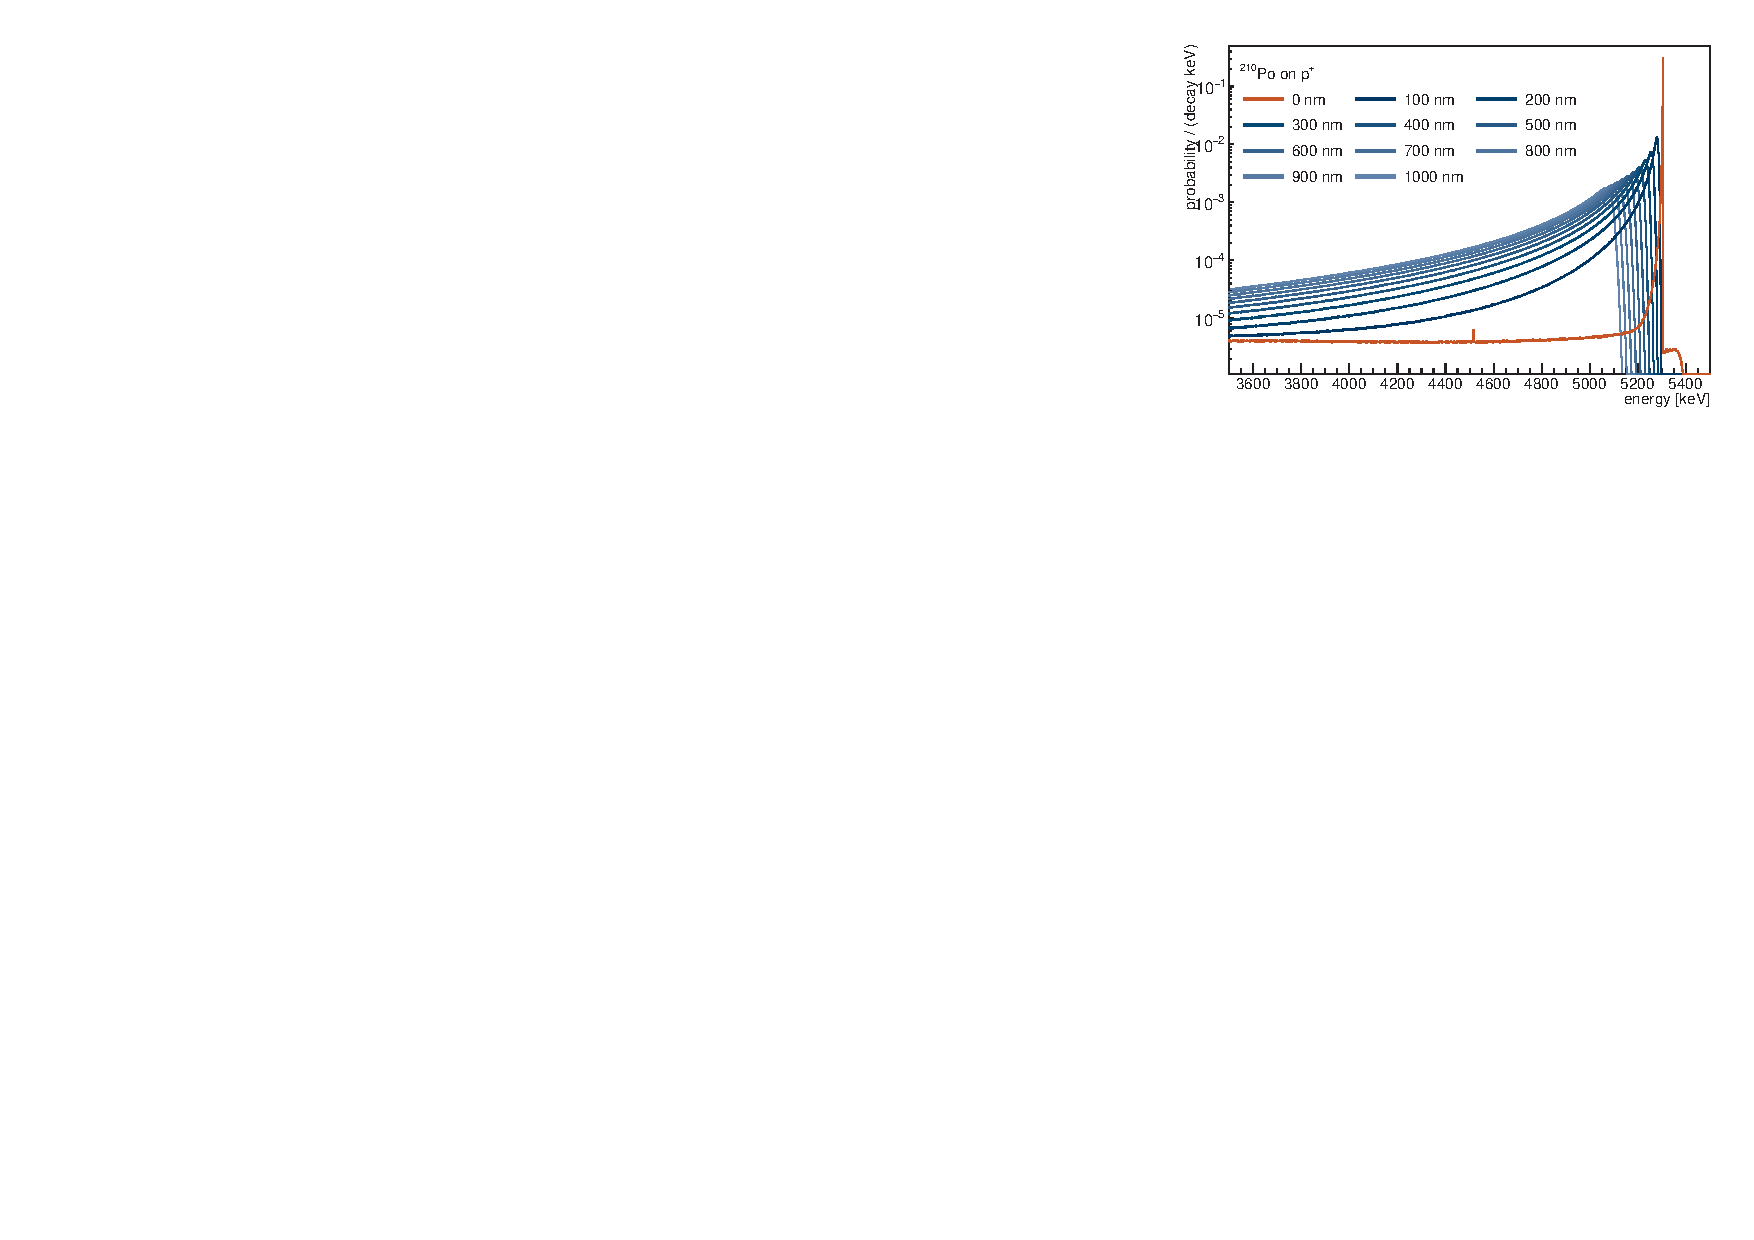
\includegraphics[width=0.48\textwidth]{plots/bkg/raw/ph2/pdfs/amodel-pdfs-Po210.pdf}}
  \hfill
  \subfloat[%
    \a\ decays from the \Ra\ decay sub-chain (\Ra, \Rn, $^{218}$Po and $^{214}$Po) on the
    detectors \pplus\ contact surface for different depths of the inactive contact layer.
    The isotope contamination is assumed to halve at each decay step, because of the
    recoil of the nuclei in LAr.\label{fig:bkg:raw:ph2:pdfs:amodel:Ra}%
  ]{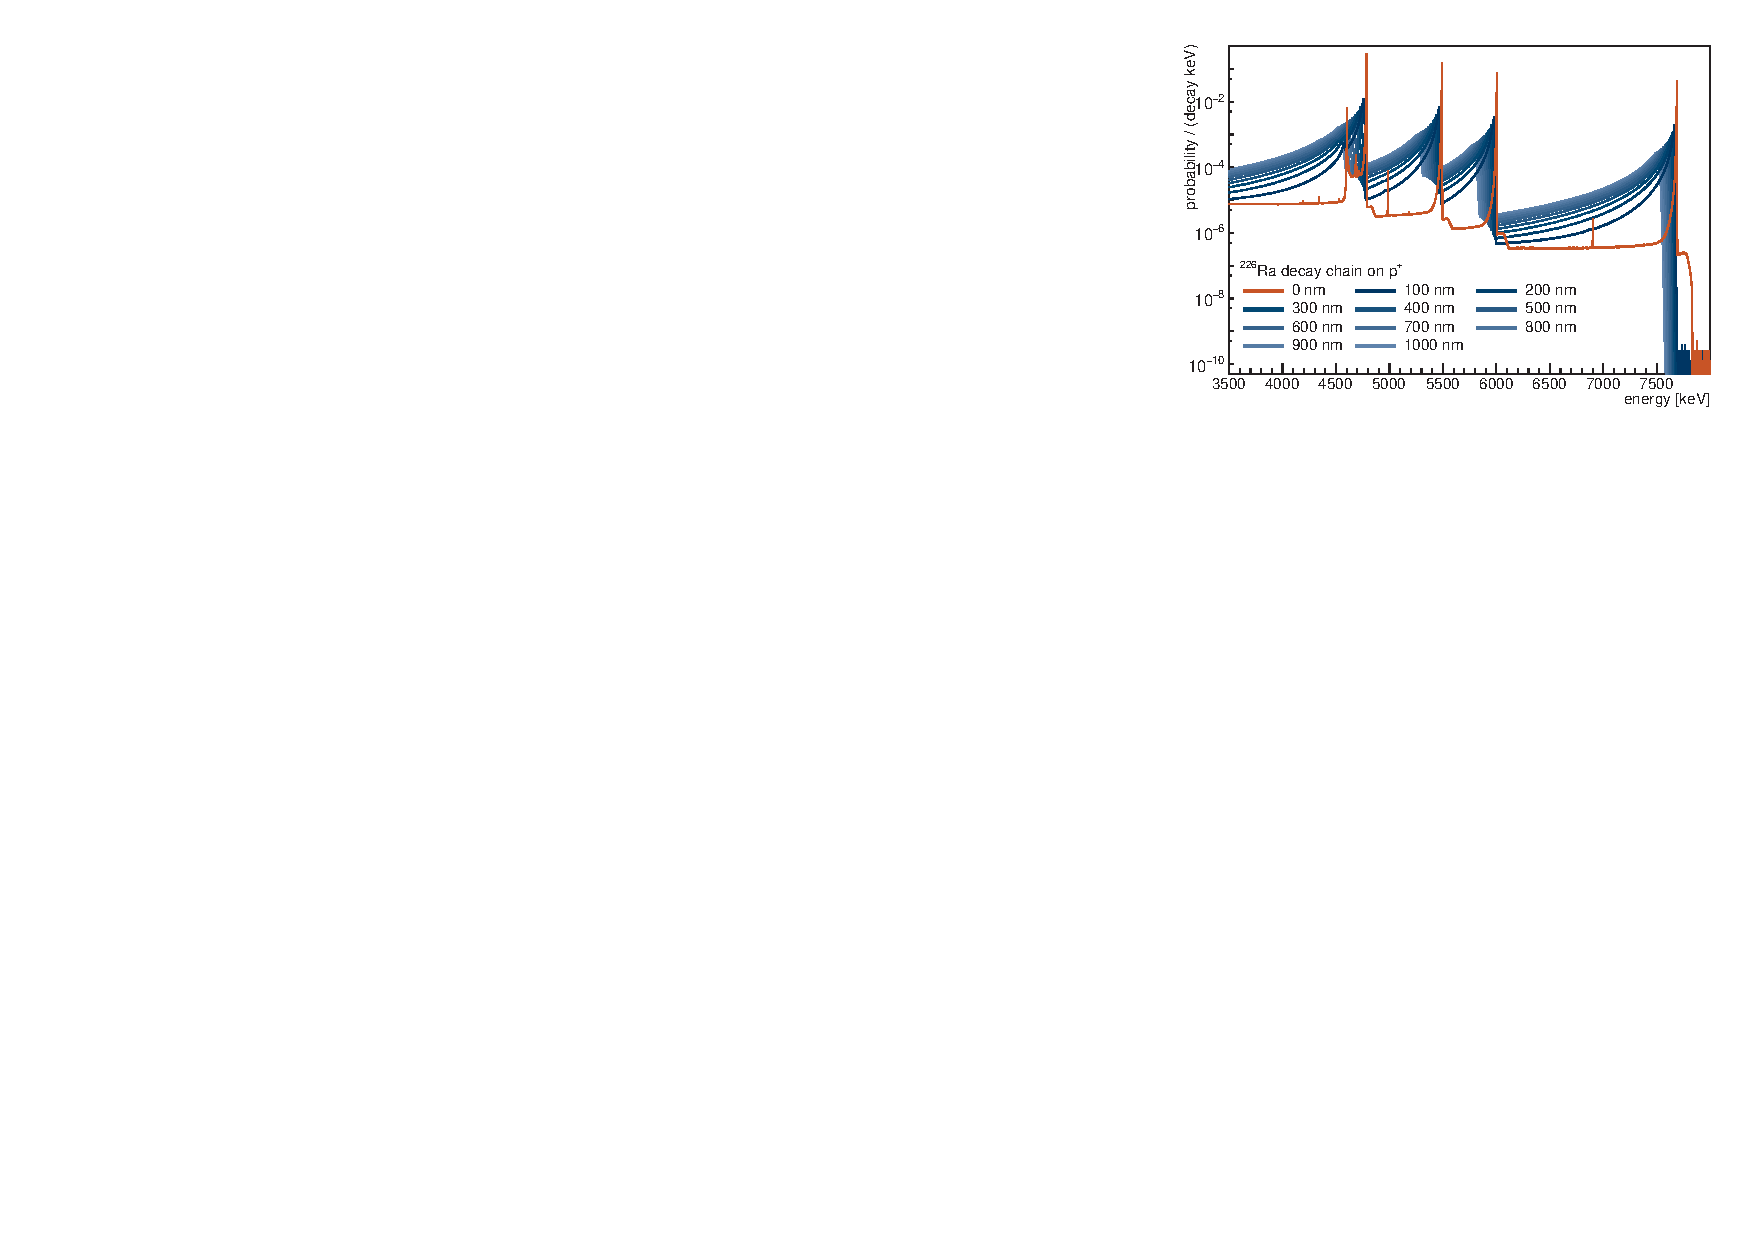
\includegraphics[width=0.48\textwidth]{plots/bkg/raw/ph2/pdfs/amodel-pdfs-U.pdf}}
  \caption{}%
  \label{fig:bkg:raw:ph2:pdfs:amodel}
\end{figure}

\blocktitle{analysis}
The likelihood function for modeling the high-energy region dominated by \a\ decays runs
only on single-detector data, namely \enrBEGeII\ and \enrCoaxII\ separately, in a range
from 3.5~MeV to 5.25~MeV. Events with an energy higher than 5.25~MeV are put in a single
overflow bin:
\begin{equation}
  \mathcal{L}_{\alpha}{(\lambda_1,\ldots,\lambda_m\,|\,n)} =
  \prod_{i=1}^{N_\text{bins}} \operatorname{P}(n_{i};\nu_{i})\;
  \label{eq:bkg:raw:ph2:amodel:likelihood}
\end{equation}
where $\operatorname{P}(n;\nu)$ denotes the Poisson probability of observing $n$ counts
with mean $\nu$. A flat prior probability is assigned to each of the fit parameters
$\lambda_i$. Both data sets are fit separately with a fixed bin size of
10~keV\footnote{%
  The calibration curves are accurate on the sub-keV level up to the highest \g\ energy of
  about 2.6~MeV emitted by the \Th\ calibration sources. Although no major non-linearity
  effects were found the same accuracy cannot be guaranteed at 6~MeV.  Deviations from
  linearity at this energy are within 10~keV, hence, we increase the bin size in the
  higher energy range.
} as the \a\ contamination is detector individual and the
two single-detector data sets are uncorrelated in the respective energy window.
\newpar
The fit results are shown in \cref{fig:bkg:raw:ph2:amodel:resultsplot} and listed in
\cref{tab:bkg:raw:ph2:amodel:results}. The \Po\ component is modeled with a combination of
\pplus\ contact thicknesses from 400 to 600~nm for the \enrBEGeII\ data set and from 300
to 700~nm for the \enrCoaxII\ data set in steps of 100~nm. Further \Po\ components are
rejected by a Bayes factor analysis.  Impurities belonging to the \Ra\ chain are mostly
located on \ANG{2} and thus a fit of the \enrCoaxII\ data set using a single \pplus\
thickness describes this component well. For the \enrBEGeII\ data set we observe a very
small number of counts for the \Ra\ chain, therefore, also in this case a single component
is sufficient. We determine a best-fit value of 100~nm and 500~nm, respectively. The
estimated \pvalue\ for \enrBEGeII\ is 0.2 whereas the \pvalue\ for \enrCoaxII\ is 0.3. The
dominant spectral component below 4.5~MeV is due to degraded \a\ events which extends down
to the ROI.

\begin{figure}
  \centering
  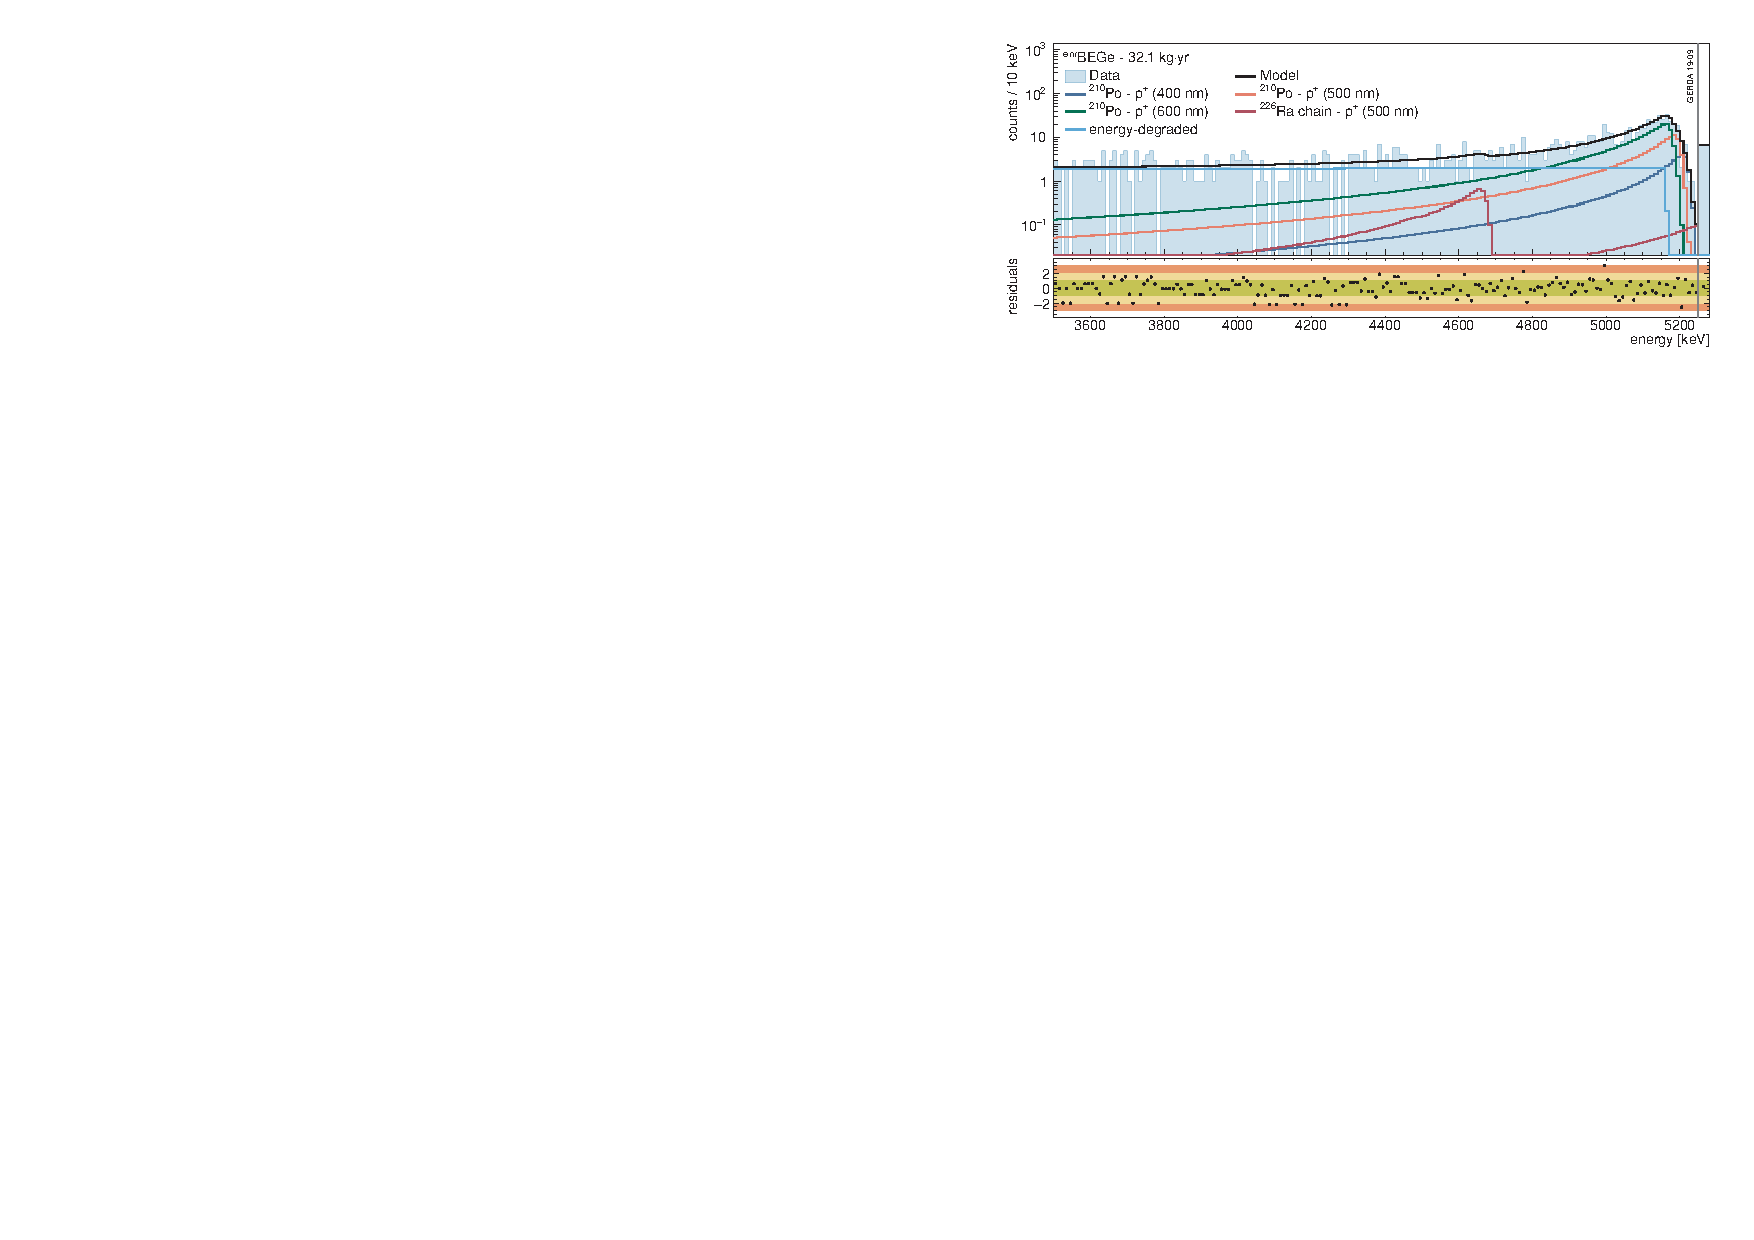
\includegraphics{plots/bkg/raw/ph2/results/amodel/amodel-enrBEGe.pdf}
  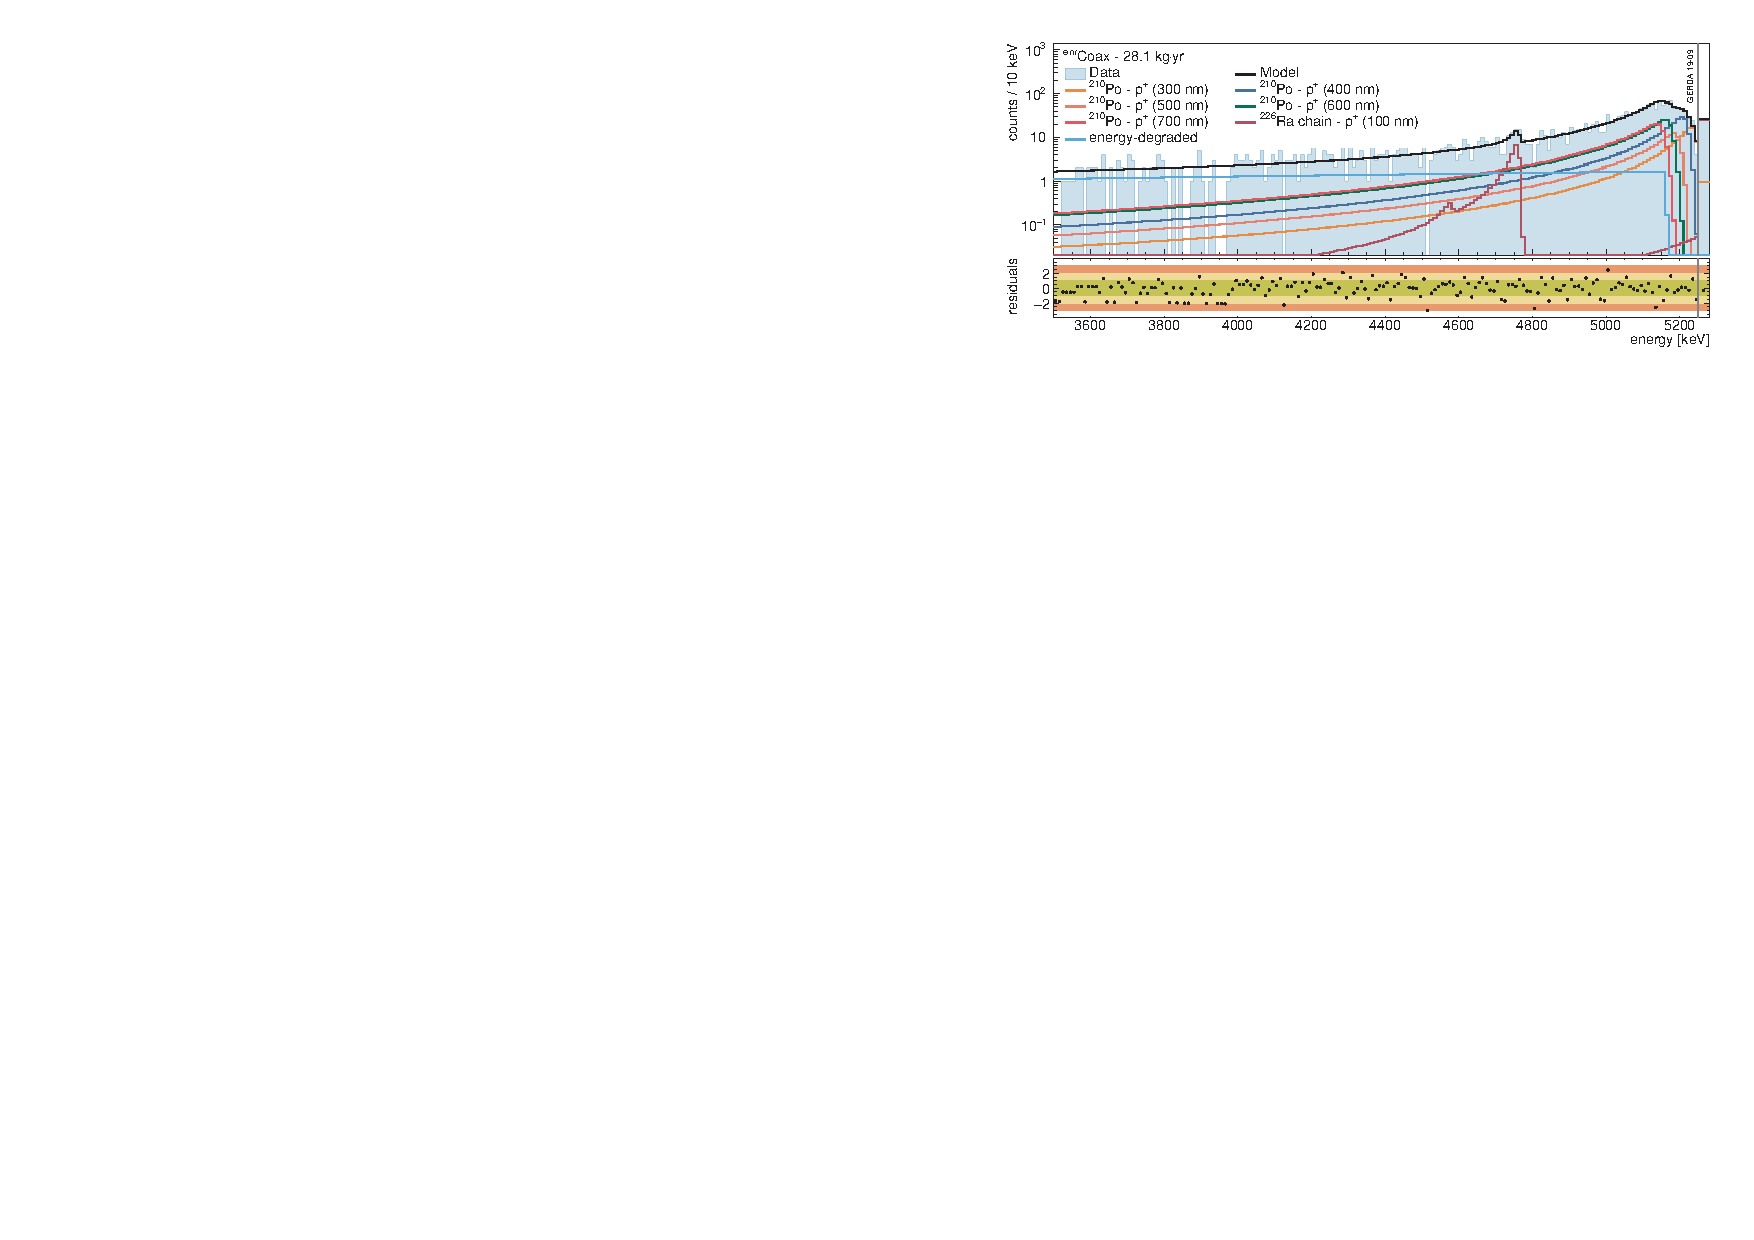
\includegraphics{plots/bkg/raw/ph2/results/amodel/amodel-enrCoax.pdf}
  \caption{%
    Fit results of the \a\ events background analysis for \enrBEGeII\
    (top) and \enrCoaxII\ (bottom). The last bin contains all events above
    5250~keV.
  }\label{fig:bkg:raw:ph2:amodel:resultsplot}
\end{figure}

\begin{table}
\centering
  \caption{%
    Fit results of the \a\ events background analysis for the
    \enrBEGeII\ and \enrCoaxII\ data sets. Values are given in counts in the
    full pdf range from 40~keV to 8000~keV.
  }\label{tab:bkg:raw:ph2:amodel:results}
  \begin{tabular}{rlccr@{ }l}
  \toprule
  \mr{2}{data set}   & \mr{2}{component} & contact & global mode & \mc{2}{marg.~mode}      \\
                     &                   & [nm]    & [cts]       & \mc{2}{68\% C.I.~[cts]} \\
  \midrule
  \mr{6}{\enrBEGeII} & \mr{4}{\Po}       & 400     & 49          & 50   & $[34,76]$        \\
                     &                   & 500     & 162         & 165  & $[107,222]$      \\
                     &                   & 600     & 346         & 342  & $[278,391]$      \\
                     &                   & comb.   & --          & 555  & $[523,586]$      \\
                     & \Ra\ chain        & 500     & 20          & 20   & $[15,29]$        \\
                     & energy-degraded   & --      & --          & 845  & $[698,948]$      \\
  \midrule
  \mr{8}{\enrCoaxII} & \mr{6}{\Po}       & 300     & 167         & 165  & $[140,208]$      \\
                     &                   & 400     & 363         & 368  & $[272,430]$      \\
                     &                   & 500     & 182         & 175  & $[83,338]$       \\
                     &                   & 600     & 433         & 420  & $[233,582]$      \\
                     &                   & 700     & 404         & 410  & $[295,537]$      \\
                     &                   & comb.   & --          & 1555 & $[1511,1609]$    \\
                     & \Ra\ chain        & 100     & 58          & 59   & $[49,70]$        \\
                     & energy-degraded   & --      & --          & 485  & $[426,599]$      \\
  \bottomrule
\end{tabular}

% vim: nowrap

\end{table}

\section{Potassium-tracking analysis}%
\label{sec:bkg:raw:ph2:kmodel}

The two full-energy lines of \kvn\ and \kvz\ at 1461~keV and 1525~keV are distinct
features of the energy spectrum shown in \cref{fig:bkg:raw:ph2:datasets}. Being a relevant
source of background for double-beta decay, the two potassium isotopes play a crucial role
in the background modeling process in \gerda. Uncertainties in their origin and
distribution propagate directly to searches for exotic physics like Majorons, Lorentz
invariance-violating processes or decay modes to excited states of \nnbb\ decay in which
the shape of the \nnbb\ decay spectrum is a unique feature and thus need to be well
understood. In the following the focus will be on the characteristics of the events
constituting these two intense \g\ lines. In order to extract information about the
spatial distribution of \kvn\ and \kvz\ contamination around the \gerda\ array, a
treatment on a detector-by-detector basis is advantageous. The two \g\ lines contain
enough statistics for such an analysis to be meaningful and constitute samples with a high
signal to background ratio.

\blocktitle{sources}
Initial observations in \phasetwo\ have shown that the \kvn\ and \kvz\ full-energy line
intensities have increased by a factor of 4 and 2, respectively, in the single-detector
data compared to \phaseone~\cite{DAndrea2017}. The \kvz\ increase in activity can be
attributed to the exchange of the mini-shrouds material from copper to nylon\footnote{%
  The exchange of material from copper to nylon has been necessary in the presence of a
  LAr veto system. Copper surfaces would have indeed blocked the scintillation light,
  instead of letting it propagate and wavelength-shift as with TPB-coated nylon
  mini-shrouds~\cite{Lubashevskiy2017}.
} during the \phasetwo\ upgrade: The electric field generated by the detectors bias high
voltage is not screened by the conductive material anymore. The \kvz\ ions can be
attracted from a larger LAr volume into the vicinity of the detectors.  Moreover, the
unshielded high-voltage cables could be an explanation for the higher rate of \kvz\ events
seen in the uppermost detectors in the \gerda\ array. The higher \kvn\ event rate, on the
other hand, is possibly attributable to the glue used for the nylon mini-shrouds and other
new materials introduced with the LAr veto system. The exact amount, location and
radio-purity of the glue is not precisely known.  All changes to the setup that have been
made during the upgrade to \phasetwo\ are described and motivated in exhaustive detail in
reference~\cite{Agostini2018a}.

\blocktitle{data set}
Data in two energy windows around the potassium \g\ lines is projected in detector index
space, such that, for single-detector data, each data point $n_i$ represents the total
counts in detector $i$ in the respective window. For two-detector data the detector space
is two-dimensional, and each data point $n_{ij}$ represents the number of events for which
energy is deposited in detector $i$ and detector $j$.  The events in the potassium lines
(denoted with \m{K40} and \m{K42} in the following) are selected in a $\pm 3\sigma$ energy
interval around the respective line, rounded up to an integer number of keV to match the
specific energy windows in the energy distributions with 1~keV binning.  $\sigma$ is the
energy resolution in the respective energy window.  Additionally, three side-bands
(\m{SB1}, \m{SB2} and \m{SB3} in the following) are used to estimate the continuum below
and above the \g\ lines. Considering the further subdivision in single- (\m{M1-}) and
two-detector (\m{M2-}) data, this leads to the definition of $5 \times 2$ energy regions,
summarized in~\cref{tab:bkg:raw:ph2:kmodel:regions-cts}. A visual representation of the
selected windows can be found in~\cref{fig:bkg:raw:ph2:kmodel:regions}. Pdfs for \Bih\ on
the flat cables and detector intrinsic \nnbb\ decays are used to estimate the background.
Other components are expected to contribute less in the respective energy windows.

\begin{table}
  \centering
  \caption{%
    Energy ranges and corresponding number of events for the potassium-tracking analysis
    (visualized in \cref{fig:bkg:raw:ph2:kmodel:regions}). Note that the windows for
    two-detector data are larger as the two single-detector energy resolutions are folded
    in the summed energy spectrum.
  }\label{tab:bkg:raw:ph2:kmodel:regions-cts}
  \begin{tabular}{ccccc}
    \toprule
             & \Mone\ [keV]  & cts. & \Mtwo\ [keV]  & cts. \\
    \midrule
    \m{K40}  & $[1457,1465]$ & 4472 & $[1455,1467]$ & 554  \\
    \m{K42}  & $[1521,1529]$ & 6718 & $[1519,1531]$ & 865  \\
    \midrule
    \m{SB1}  & $[1405,1450]$ & 1852 & $[1405,1450]$ & 452  \\
    \m{SB2}  & $[1470,1515]$ & 1124 & $[1470,1515]$ & 326  \\
    \m{SB3}  & $[1535,1580]$ & 533  & $[1535,1580]$ & 41   \\
    \bottomrule
  \end{tabular}
\end{table}

\begin{figure}
  \centering
  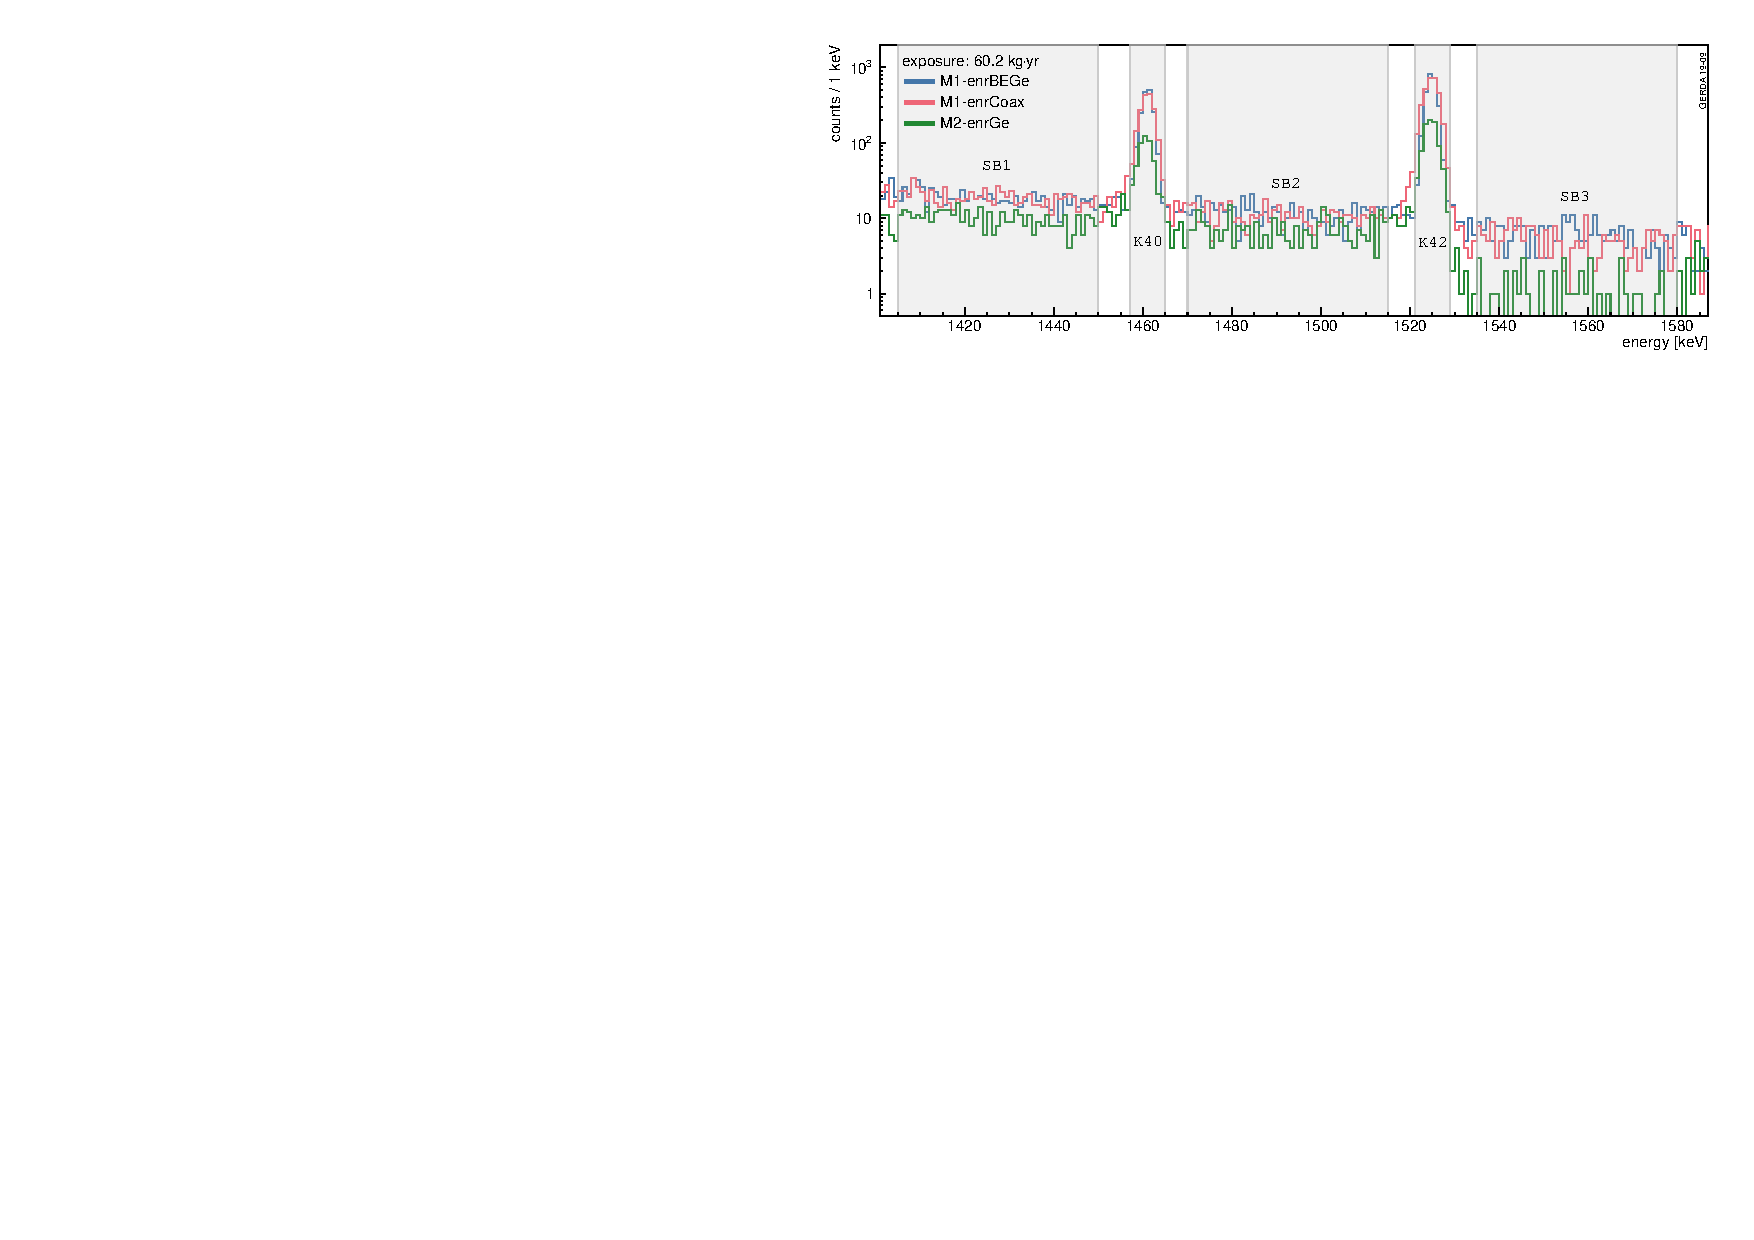
\includegraphics[width=0.8\linewidth]{plots/bkg/raw/ph2/kmodel-regions.pdf}
  \caption{%
    Visual representation of the five energy ranges defined for the potassium-tracking
    analysis. The exact intervals and counts are given in
    \cref{tab:bkg:raw:ph2:kmodel:regions-cts}.
  }\label{fig:bkg:raw:ph2:kmodel:regions}
\end{figure}

\blocktitle{likelihood}
The statistical approach of factorizing the likelihood is described in
\cref{sec:bkg:raw:ph2:stat}. The part of the likelihood analyzed here runs simultaneously
on the $5 \times 2$ energy ranges presented above. Following the previously introduced
naming convention introduced it reads:
\begin{equation}\label{eq:bkg:raw:ph2:kmodel:likelihood}
  \mathcal{L}_\text{K}(\lambda_1,\ldots,\lambda_{m'}\,|\,n) =
  \prod_{d=1}^{N_\text{dat}}
  \left\{
    \prod_{i=1}^{N_\text{det}}
    \operatorname{P}(n_{d,i}^\text{\m{M1}};\nu_{d,i}^\text{\m{M1}})
    \times
    \prod_{j<k}^{N_\text{det}}
    \operatorname{P}(n_{d,jk}^\text{\m{M2}};\nu_{d,jk}^\text{\m{M2}})
  \right\}\;,
\end{equation}
where the index $i$ runs over the bins (i.e.~detectors) and the index $d$ over the 5
considered energy windows, namely the three side-bands \m{SB1}, \m{SB2}, \m{SB3} and the
two line-bands \m{K40} and \m{K42}.  The \m{M2-} data sets are two-dimensional in detector
space and run over the two indices $j$ and $k$. $\operatorname{P}(n,\nu)$ is the usual
Poisson probability.

\blocktitle{priors}
Gaussian prior probability distributions for the \kvn\ activity are built from
radio-purity screening measurements (see \cref{apdx:assay}). For \kvz, for which no
screening information is available, uniform priors are adopted, with the exception of the
two \kvz\ components located on the \nplus\ contact surface of \bege\ and \scoax\
detectors. \kvz\ can be attracted to the \nplus\ surface by the electrical field created
by the high voltage potential applied to the detectors. Both components are expected to be
correlated by the volume ratio of the mini-shrouds (3:2 \bege\ to \scoax) the \kvz\ ions
are attracted from. The volume ratio estimate is extracted from the geometric
implementation in \mage.  We assume an uncertainty of 0.1~mBq on either activity allowing
for a change of their ratio. The correlation is included in the fit via a two-dimensional
prior.

\blocktitle{base \\ model}
The analysis flow starts with a construction of a first, preliminary model, which consists
only of background contributions that are expected from screening measurements of \kvn\
and known properties of \kvz.  The resulting model, however, gives a non-satisfactory
description of data and the posterior distributions for the \kvn\ components are
significantly shifted to higher values with respect to the prior distributions, indicating
a surplus of \kvn.  To find a better agreement with physics data while keeping the model
as simple as possible, additional components using uniform priors are included one at a
time in the fitting procedure, and the Bayes factor is calculated between the extended and
the preliminary model. The model is iteratively updated by adding the component that
results in the highest Bayes factor until no Bayes factor is larger than 10.
\newpar
In a first iteration a replica of the pdf of \kvn\ in the mini-shrouds is added obtaining
a Bayes factor~$\gg$10. \kvn\ in the Tetratex\reg-coated copper shrouds is added in a
second iteration with a Bayes factor of 11.  For \kvz\ the only additional component that
results in a Bayes factor greater than 1 is \kvz\ on the \nplus\ detector contacts.
Although the fit shows only a slight preference (Bayes factor of 2) the component is added
to the model because of its importance in the full-range fit, where the energy region
above the 1525~keV \g\ line is also considered.  The results of the base model are shown
in \cref{tab:bkg:raw:ph2:kmodel:base:results} and a graphic representation showing the
counts per detector in both potassium \g\ lines in \Mone\ and \Mtwo\ data can be found in
\cref{fig:bkg:raw:ph2:kmodel:base:results}. The complete selection of plots is available
in \cref{apdx:kmodelplots}.  The analysis yields a \pvalue\ of $\sim$0.07, indicating an
acceptable description of the data. To further improve the model rotationally asymmetric
fit components are needed. The base model is accurate enough to be used as input for the
full-range fit, which is insensitive to any rotational inhomogeneity of the location of
background sources, as spectra from different detectors are merged into a single data set.

\begin{figure}
  \centering
  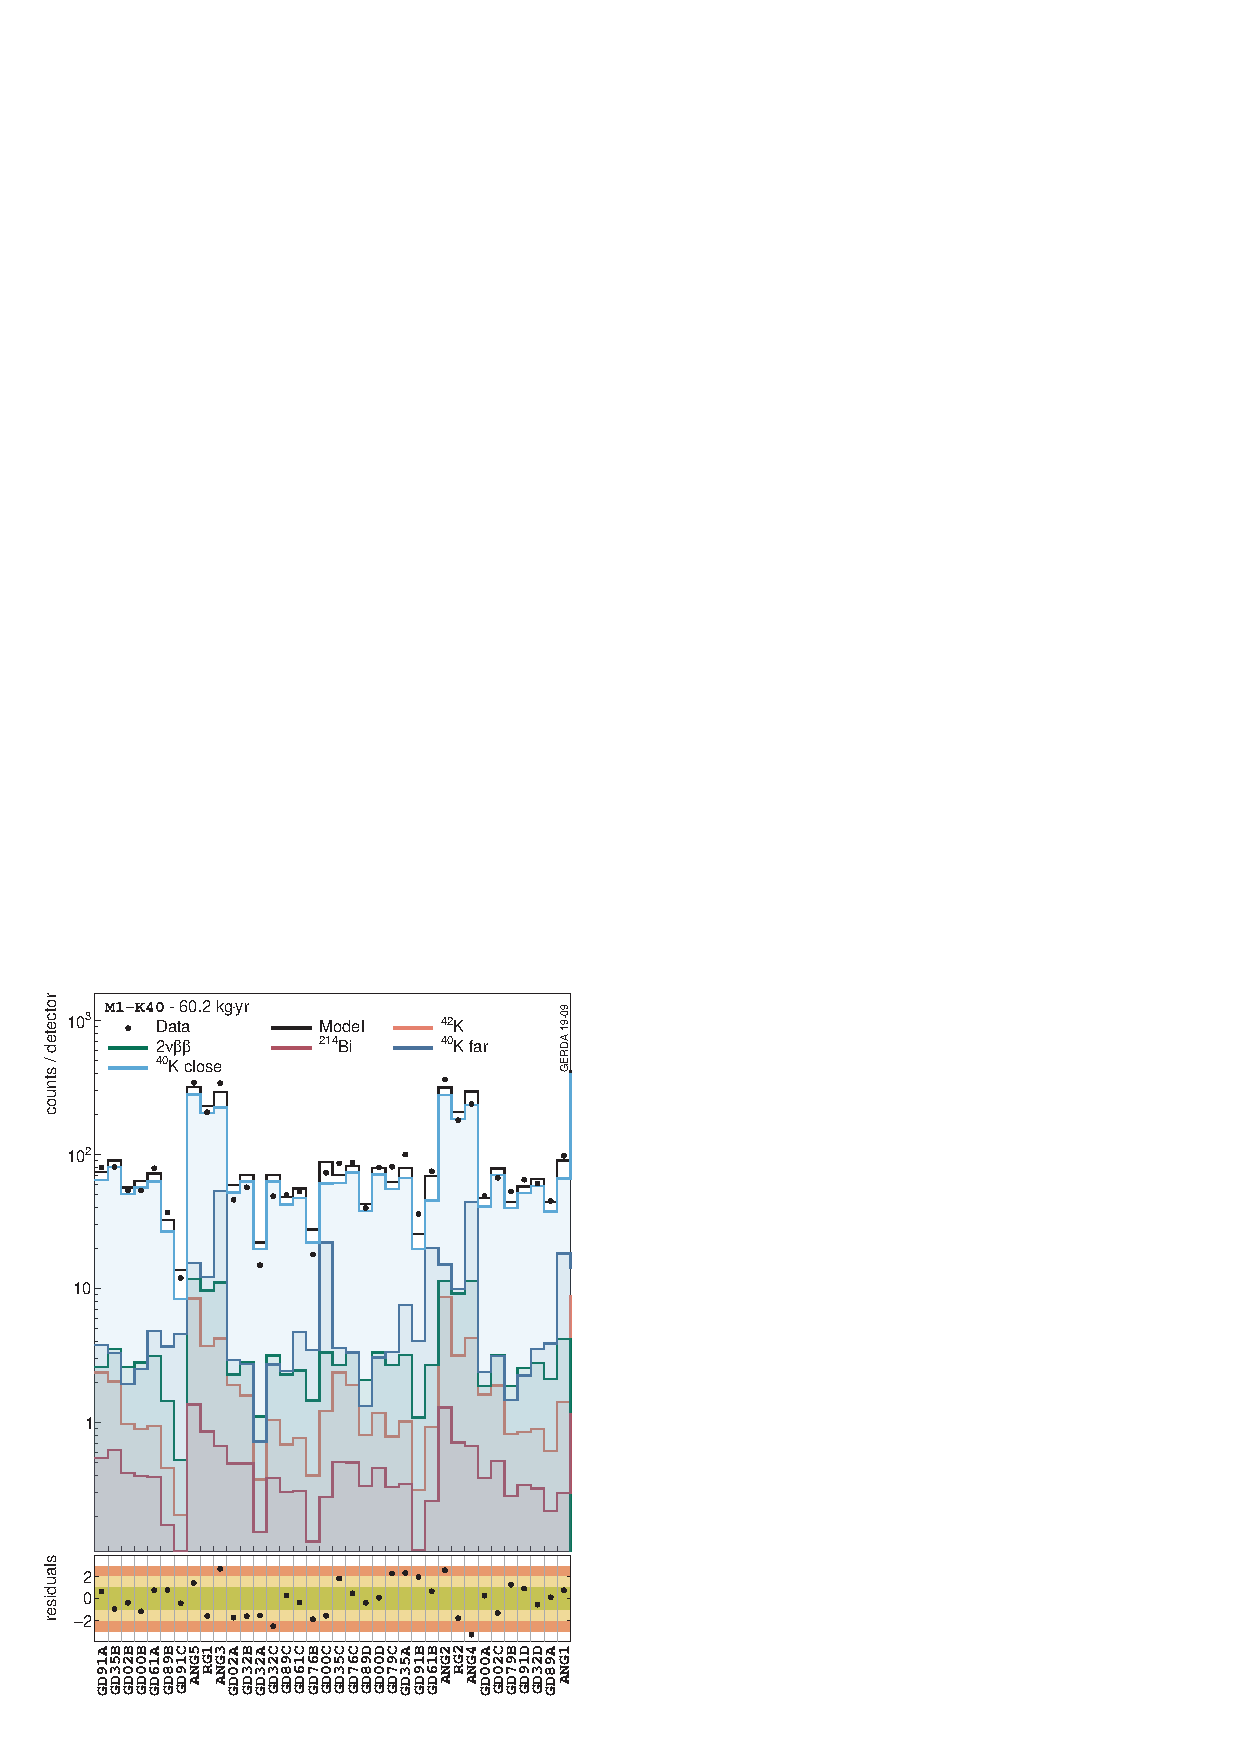
\includegraphics[width=0.45\linewidth]{plots/bkg/raw/ph2/results/kmodel/kmodel-1d-ds0.pdf}
  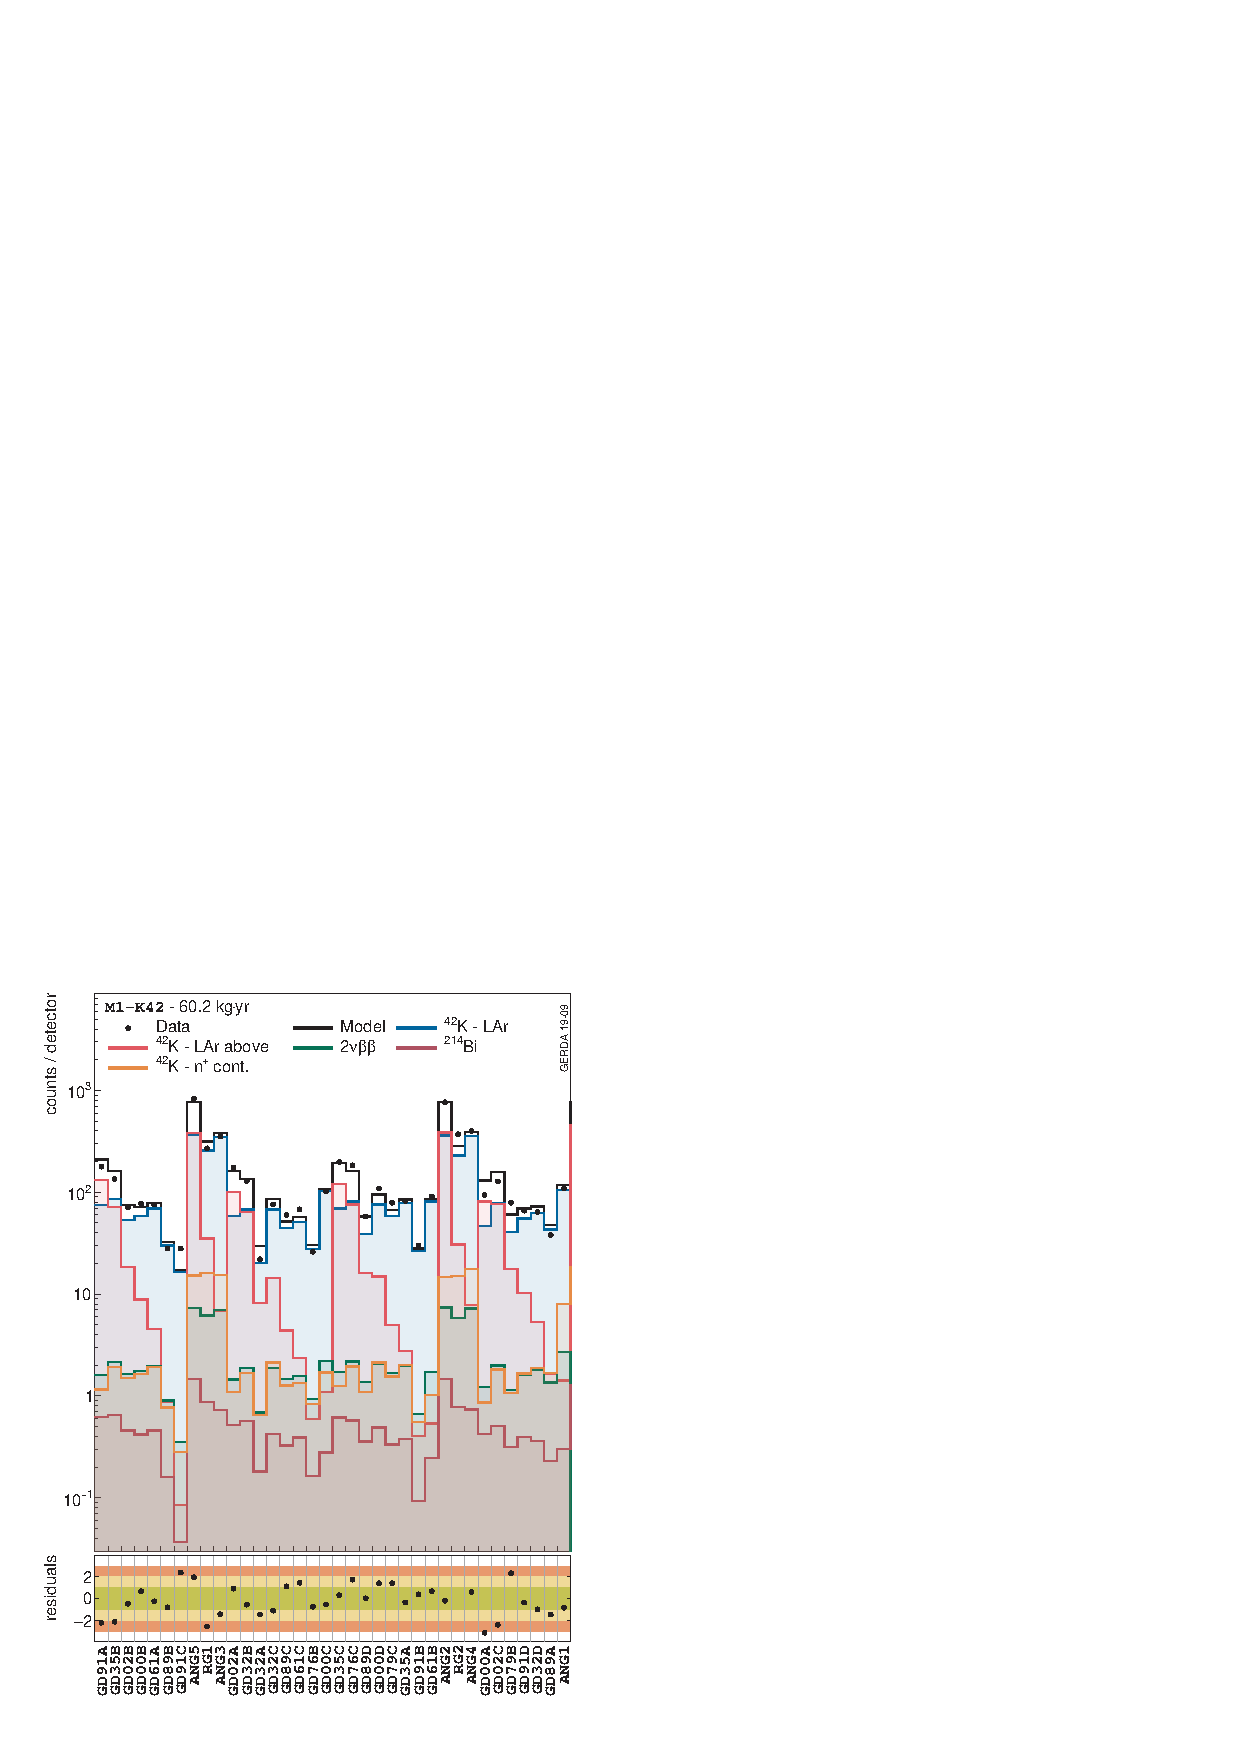
\includegraphics[width=0.45\linewidth]{plots/bkg/raw/ph2/results/kmodel/kmodel-1d-ds1.pdf}
  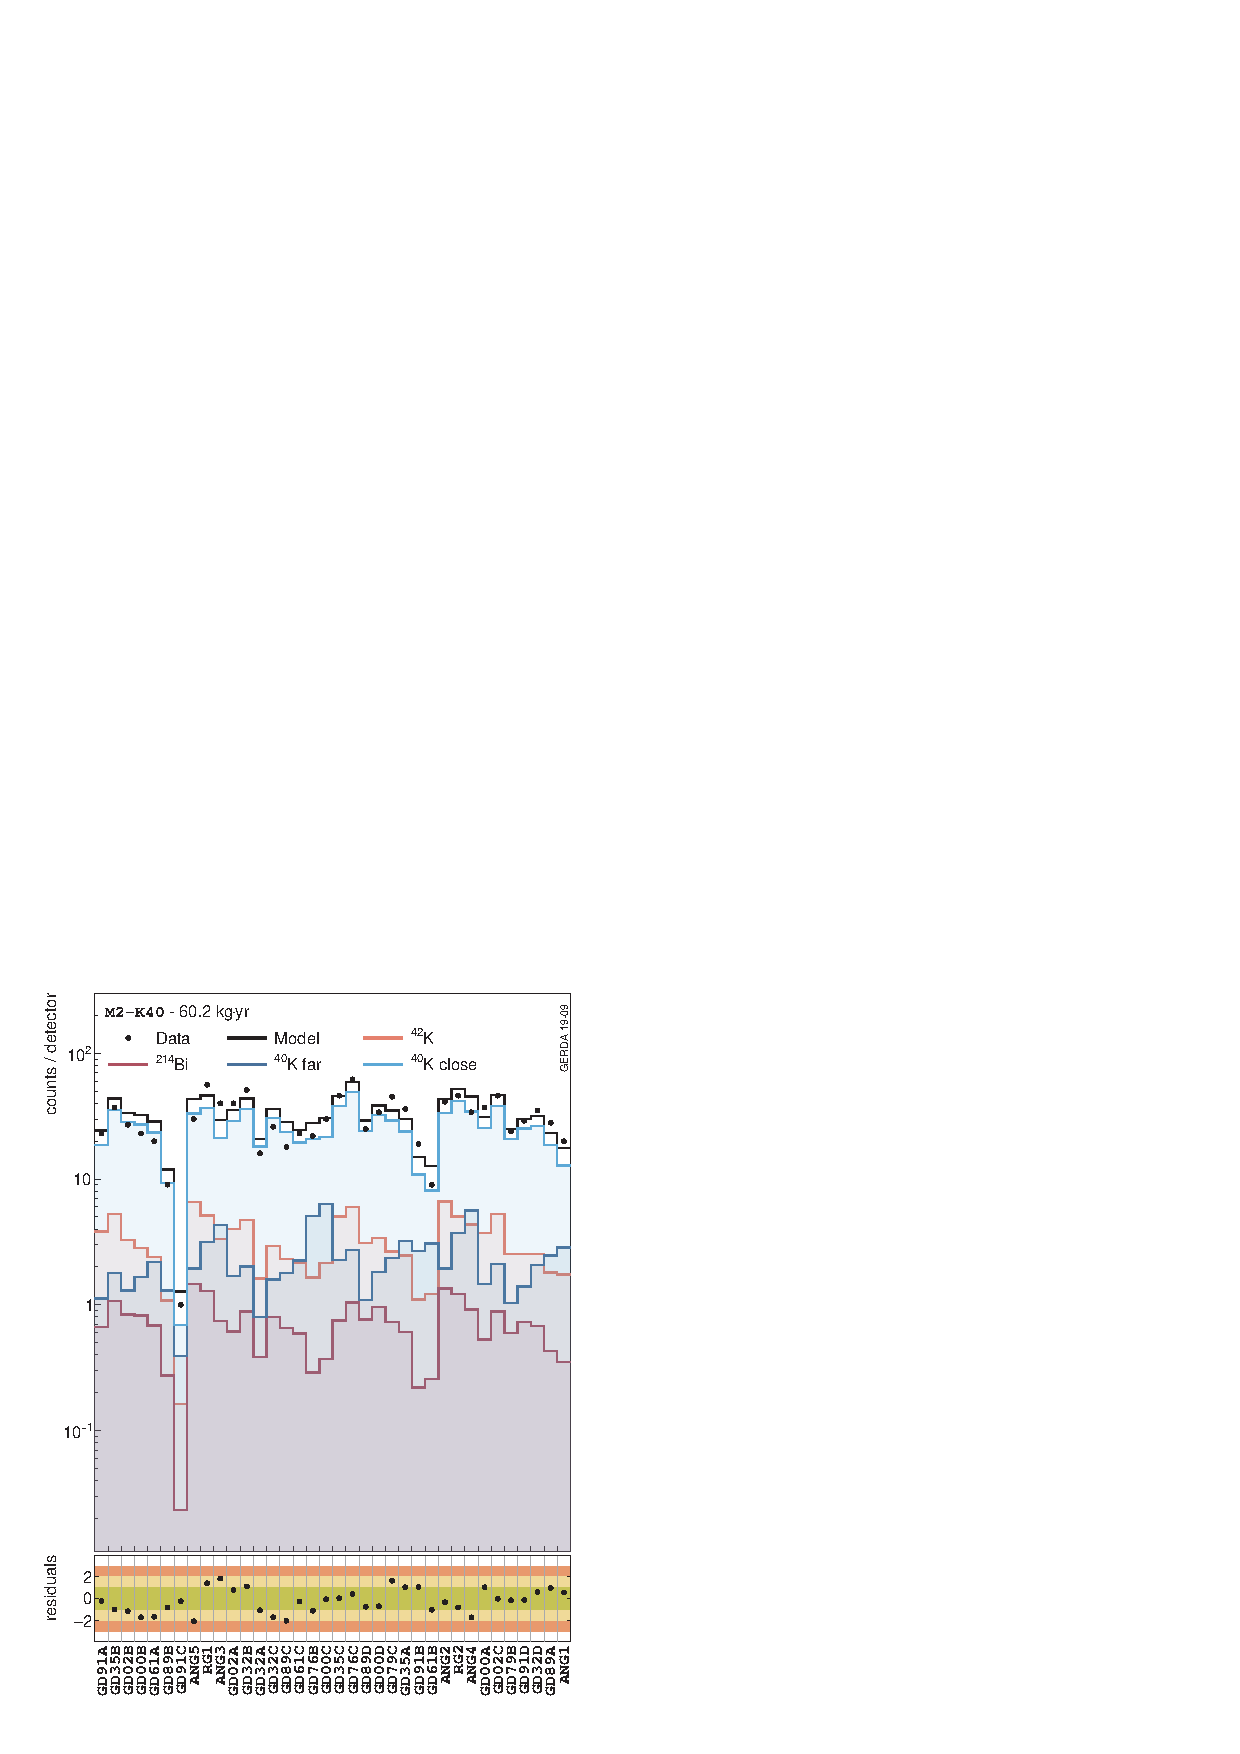
\includegraphics[width=0.45\linewidth]{plots/bkg/raw/ph2/results/kmodel/kmodel-2d-ds5.pdf}
  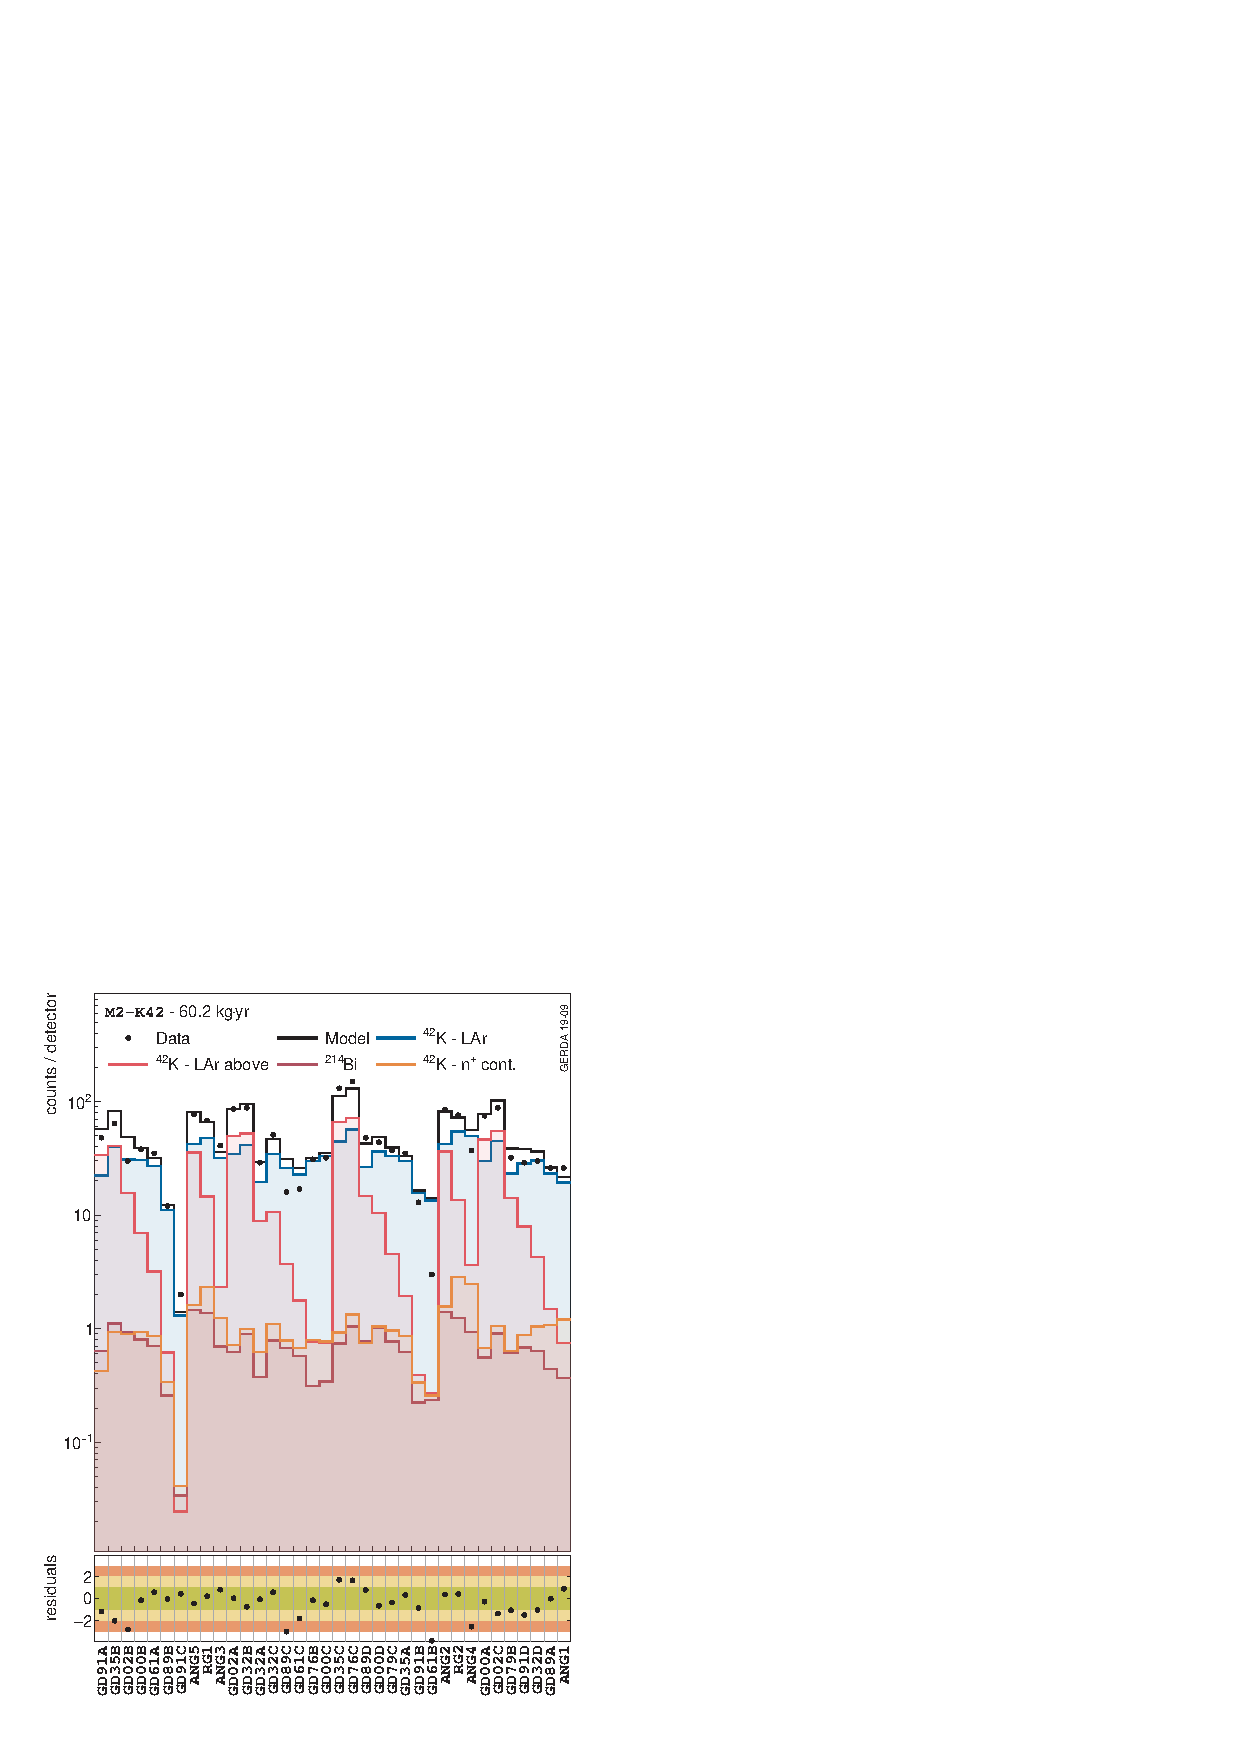
\includegraphics[width=0.45\linewidth]{plots/bkg/raw/ph2/results/kmodel/kmodel-2d-ds6.pdf}
  \caption{%
    Decomposition of the energy windows corresponding to the two potassium lines in
    detector space: single-detector data (top) one-dimensional representation of
    two-detector data (bottom). Some components are merged for visualization purposes: in
    the \m{K40} plots combined components are shown for \kvz\ and \Bih, while \kvn\
    sources are grouped in close (flat cables, holders, mini-shrouds) and far (fibers,
    SiPMs, copper shrouds, front-end electronics) locations from the detector array. To
    visualize the two-detector data the sum of the projections on the two domain axes
    (index $i$ and index $j$) is shown.
  }\label{fig:bkg:raw:ph2:kmodel:base:results}
\end{figure}

\begin{table}
  \centering
  \caption{%
    Summary of the fit parameters estimated with the potassium source tracking analysis
    (base model). The type of prior distribution is indicated with \m{[f]}: flat, \m{[g]}:
    Gaussian. ($\,^{\dagger}$ Tetratex\reg-coated)
  }\label{tab:bkg:raw:ph2:kmodel:base:results}
  \begin{tabular}{rlcccc}
  \toprule
  \mr{2}{source} & \mr{2}{\m{[prior]} location}        & \mr{2}{units} & global & marg. & 68\% C.I. or    \\
                 &                                     &               & mode   & mode  & 90\% upper C.L. \\
  \midrule
  \mr{9}{\kvn}   & \m{[g]} flat cables                 & \mr{9}{mBq}   & 3.29   & 3.25  & $[1.79, 4.72]$  \\
                 & \m{[g]} front-end electronics       &               & 15.7   & 15.9  & $[11.1, 20.1]$  \\
                 & \m{[g]} copper shrouds$^{\dagger}$  &               & 18.4   & 18.1  & $[16.6, 20.0]$  \\
                 & \m{[g]} fiber shroud                &               & 2.82   & 2.81  & $[2.24, 3.38]$  \\
                 & \m{[g]} detector holders            &               & 1.73   & 1.73  & $[1.28, 2.14]$  \\
                 & \m{[g]} mini-shrouds                &               & 1.70   & 1.70  & $[1.60, 1.80]$  \\
                 & \m{[g]} SiPM ring                   &               & 2.50   & 2.73  & $[0.83, 4.13]$  \\
                 & \m{[f]} far from the array          &               & 328    & 322   & $[232,  416]$   \\
                 & \m{[f]} close to the array          &               & 10.8   & 10.8  & $[9.53, 12.1]$  \\
  \midrule
  \mr{4}{\kvz}   & \m{[f]} \nplus\ (BEGe)              & \mr{4}{mBq}   & 0      & 0     & < 0.37          \\
                 & \m{[f]} \nplus\ (Coax)              &               & 0.22   & 0.24  & $[0.12, 0.38]$  \\
                 & \m{[f]} LAr -- above array          &               & 450    & 454   & $[436,  470]$   \\
                 & \m{[f]} LAr -- outside mini-shrouds &               & 2036   & 2009  & $[1915, 2080]$  \\
  \midrule
  \Bih\          & \m{[g]} flat cables                 & mBq           & 1.51   & 1.26  & $[0.93, 1.51]$  \\
%                & \m{[g]} detector holders            &               & 0      & 0     & < 0.35          \\
  \midrule
  \nnbb\         & \m{[f]} germanium                   & $10^{21}$yr   & 1.91   & 1.93  & $[1.86, 2.00]$  \\
  \bottomrule
\end{tabular}

% vim: nowrap

\end{table}

\blocktitle{extended \\ model}
The two components \emph{\kvn\ close to the array} and \emph{\kvz\ in LAr above the array}
are split into 7 sub-components on a string-by-string basis (for the respective pdfs see
\cref{apdx:magepdfs}). Furthermore, we consider a \kvn\ contamination on top of the
central mini-shroud.  The results of this extended analysis are listed in
\cref{tab:bkg:raw:ph2:kmodel:extended:results}. The reader is referred to
\cref{apdx:kmodelplots} for the graphical representation of the background decomposition.
Per-string concentrations of \kvn\ and \kvz\ are visualized also in
\cref{fig:bkg:raw:ph2:kmodel:extended:strings}.  An elevated \kvz\ concentration is found
above the central string while a lower concentration is observed above the adjacent
strings \m{S1} and \m{S6} (string numbers follow the nomenclature used in
\cref{fig:setup:array}). Due to the large number of components the fit yields a high
anti-correlation between the \kvz\ concentration above the outer strings and \m{S7}. This
results in a high uncertainty on the latter fit parameter.
\newpar
The screening measurements do not account for all observed \kvn. In general ICP-MS
screening of the mini-shrouds with respect to \kvn\ is difficult and yielded only a lower
limit. Different measurements seem to indicate different contamination levels of different
mini-shrouds.  Samples of glued nylon yielded the highest potassium contamination. As the
gluing of the nylon mini-shrouds is done manually during installation the amount of glue
and its exact location is hard to control. Hence, an asymmetric distribution is expected.
The \kvn\ content of other close components like holders and cables might also be
asymmetric. The asymmetric \kvn\ contamination is confirmed by the extended potassium
tracking analysis. Also, an additional \kvn\ distribution on the top-lid of the central
mini-shroud is preferred.  The surplus in the far \kvn\ component instead is possibly explained
by setup parts omitted in the model like the PMTs and voltage-dividers of the LAr veto
system. An upper limit of their \kvn\ content, <330~mBq, was estimated from material
screening which is similar to the activity reconstructed for the far \kvn\ component. The
location of the PMTs with respect to the detector array is very similar to the
Tetratex\reg-coated copper-shrouds and their pdfs are, hence, degenerate.

\begin{table}
  \centering
  \caption{%
    Summary of the fit parameters estimated with the potassium source tracking analysis
    (extended model). The type of prior distribution is indicated with \m{[f]}: flat,
    \m{[g]}: Gaussian. ($\,^{\dagger}$ Tetratex\reg-coated)
  }\label{tab:bkg:raw:ph2:kmodel:extended:results}
  \begin{tabular}{rlcccc}
  \toprule
  \mr{2}{source} & \mr{2}{\m{[prior]} location}        & \mr{2}{units} & global & marg. & 68\% C.I. or    \\
                 &                                     &               & mode   & mode  & 90\% upper C.L. \\
  \midrule
  \mr{16}{\kvn}  & \m{[g]} flat cables                 & \mr{16}{mBq}  & 2.33   & 1.08  & $[0.13,2.30]$   \\
                 & \m{[g]} front-end electronics       &               & 14.5   & 14.4  & $[10.2,18.7]$   \\
                 & \m{[g]} copper shrouds$^{\dagger}$  &               & 18.4   & 18.5  & $[16.6,20.0]$   \\
                 & \m{[g]} fiber shroud                &               & 2.83   & 2.77  & $[2.24,3.38]$   \\
                 & \m{[g]} detector holders            &               & 2.57   & 2.29  & $[1.75,2.78]$   \\
                 & \m{[g]} mini-shrouds                &               & 1.70   & 1.70  & $[1.60,1.79]$   \\
                 & \m{[f]} close to \m{S1}             &               & 0.81   & 0.83  & $[0.47,1.28]$   \\
                 & \m{[f]} close to \m{S2}             &               & 2.35   & 2.22  & $[1.83,2.51]$   \\
                 & \m{[f]} close to \m{S3}             &               & 0      & 0     & < 0.50          \\
                 & \m{[f]} close to \m{S4}             &               & 2.58   & 2.55  & $[2.10,3.02]$   \\
                 & \m{[f]} close to \m{S5}             &               & 0.97   & 0.85  & $[0.56,1.16]$   \\
                 & \m{[f]} close to \m{S6}             &               & 1.86   & 1.89  & $[1.46,2.30]$   \\
                 & \m{[f]} close to \m{S7}             &               & 0      & 0     & < 2.92          \\
                 & \m{[f]} \m{S7} mini-shroud (top)    &               & 2.09   & 1.83  & $[1.26,2.40]$   \\
                 & \m{[g]} SiPM ring                   &               & 2.44   & 2.32  & $[0.83,4.02]$   \\
                 & \m{[f]} far from the array          &               & 390    & 374   & $[280,468]$     \\
  \midrule
  \mr{10}{\kvz}  & \m{[f]} \nplus\ (BEGe)              & \mr{10}{mBq}  & 0.15   & 0.19  & $[0.05,0.37]$   \\
                 & \m{[f]} \nplus\ (Coax)              &               & 0.22   & 0.26  & $[0.12,0.41]$   \\
                 & \m{[f]} LAr -- above \m{S1}         &               & 0      & 0     & < 0.80          \\
                 & \m{[f]} LAr -- above \m{S2}         &               & 2.22   & 2.96  & $[2.21,3.63]$   \\
                 & \m{[f]} LAr -- above \m{S3}         &               & 1.20   & 1.57  & $[1.06,2.16]$   \\
                 & \m{[f]} LAr -- above \m{S4}         &               & 1.43   & 1.89  & $[1.33,2.41]$   \\
                 & \m{[f]} LAr -- above \m{S5}         &               & 1.49   & 1.91  & $[1.38,2.73]$   \\
                 & \m{[f]} LAr -- above \m{S6}         &               & 0      & 0     & < 1.21          \\
                 & \m{[f]} LAr -- above \m{S7}         &               & 10.4   & 7.84  & $[4.95,9.83]$   \\
                 & \m{[f]} LAr -- outside mini-shrouds &               & 2083   & 2058  & $[1960,2145]$   \\
  \midrule
  \Bih\          & \m{[g]} flat cables                 & mBq           & 1.60   & 1.41  & $[1.14,1.66]$   \\
%                & \m{[g]} detector holders            &               & 0      & 0     & < 0.26          \\
  \midrule
  \nnbb\         & \m{[f]} germanium                   & $10^{21}$yr   & 1.89   & 1.89  & $[1.83,1.97]$   \\
  \bottomrule
\end{tabular}

\end{table}

\begin{figure}
  \centering
  \includegraphics[width=0.7\textwidth]{plots/bkg/raw/ph2/results/kmodel/kmodel-asym.pdf}
  \caption{%
    Asymmetry of \kvn\ contaminations (left) close to the array strings (for \m{S7} just
    on the top-lid) and \kvz\ (right) above the detector strings. The inner and outer
    radii of each circle are proportional to the edges of the smallest 68\% C.I. of the
    marginalized posterior distributions. The numerical values can be found in
    \cref{tab:bkg:raw:ph2:kmodel:extended:results}.
  }\label{fig:bkg:raw:ph2:kmodel:extended:strings}
\end{figure}

\section{Full-range analysis}%
\label{sec:bkg:raw:ph2:gmodel}

As described in \cref{sec:bkg:raw:ph2:stat} the \a-event background and
potassium \g\ lines are studied individually and the results are incorporated in the
full-range fit as prior distributions.  The latter consists in a simultaneous fit of the
\Mone\ and the \Mtwo\ data sets. For the final combination of parameters, outlined in this
section, components with a posterior distribution peaked at zero were removed from the
fit. The stability of the results with respect to the bin size and prior distributions was
verified. Changing the prior distribution for fit parameters for which no screening
measurement is available from a flat to an exponential one does not significantly impact
the final posterior distributions. The compatibility of the final model, which includes 34
fit parameters, with data is supported by a \pvalue\ of $\sim$~0.3.
\newpar
The estimated activities of individual components and other parameters of interest are
listed in \cref{tab:bkg:raw:ph2:gmodel:results}. In particular, for each component we
report the global and the marginalized mode of the posterior parameter distribution, along
with its smallest 68\% C.I. The global mode corresponds to the global best fit value while
the marginalized mode is the most probable parameter value when integrating over all other
parameters. The original type of prior distribution is marked with \m{[f]} for flat,
\m{[g]} for Gaussian and \m{[e]} for exponential; the latter two are used if screening
measurements are available. Subsequently, for all \kvn\ and \kvz\ components, the prior
distribution is imported from the potassium-tracking analysis and for \Pbh\ and \Bih\ on
the \pplus\ contact from the reconstructed \Ra\ content from the \a\ events background
analysis.
\newpar
The spectral decomposition of all data sets is shown in
\cref{fig:bkg:raw:ph2:gmodel:results}. For each data set the residual distribution as a
multiple of the expected 1$\sigma$ fluctuation in each bin (i.e.~the 68\% probability
interval centered on the mean of the Poisson distribution) is displayed. We find for the
\enrBEGeII\ data set 66.4\%, 94.5\% and 99.6\% of points in the 1$\sigma$-, 2$\sigma$- and
3$\sigma$-bands, for the \enrCoaxII\ data set 66.0\%, 94.7\% and 99.8\% and for the
\enrGeII\ data set 70.0\%, 96.1\% and 99.7\%, respectively. Thus, in all three cases the
residuals are normally distributed. No outliers with residuals larger than $3\sigma$ are
found in a $\pm50$~keV window around \qbb\ and the bins exceeding $3\sigma$ do not
correspond to any known \g\ line.

\begin{sidewaystable}
  \centering
  \footnotesize
  \caption{%
    Summary of the analysis parameter estimates. Global mode and marginalized mode, along
    with its smallest 68\% C.I., are reported as representatives of the posterior
    parameter distribution. The number of reconstructed counts in the fit range and the
    background index at \qbb\ prior active background suppression are listed for each
    component and each analysis data set. The original type of prior distribution is
    marked with \m{[f]} for flat, \m{[g]} for Gaussian and \m{[e]} for exponential.
    ($\,^{\dagger}$ Tetratex\reg-coated)
  }\label{tab:bkg:raw:ph2:gmodel:results}
  \newcolumntype{H}{>{\setbox0=\hbox\bgroup}c<{\egroup}@{}}
\newcolumntype{x}[1]{>{\centering\arraybackslash}p{#1}}
\newcommand{\mrr}[2]{\multirow{#1}[1]{*}{#2}}
\newcommand{\mrc}[2]{\multirowcell{#1}{#2}}

\begin{tabular}{%
  r
  l
  c
  S[% global mode
    table-format=4.2,
    table-number-alignment=right,
    table-text-alignment=right,
    table-parse-only
  ]
  r@{ }l% marginalized with 68% CI interval
  S[% screening measurements
    table-number-alignment=left,
    table-text-alignment=left,
    table-parse-only
  ]
  S[% BEGe
    table-format=5.0,
    table-number-alignment=center,
    table-text-alignment=center,
    table-auto-round=true
  ]@{ | }
  l
  S[% Coax
    table-format=4.0,
    table-number-alignment=center,
    table-text-alignment=right,
    table-auto-round
    ]@{ | }
  l
  S[% M2-All
    table-format=4.0,
    table-number-alignment=center,
    table-text-alignment=center,
    table-auto-round
  ]
}
  \toprule
  \mrr{3}{source}      & \mrr{3}{\m{[prior]} location}         & \mrr{3}{units}      & {\mrc{3}{global\\mode}} & \mc{2}{\mrc{3}{marg.~mode\\with 68\% CI}} & {\mrr{3}{screening}} & \mc{5}{model content in fit range | BI at \qbb}                                             \\
                       &                                       &                     &                         &       &                                   &                      & \mc{5}{units: cts | $10^{-3}$\ctsper}                                                       \\
  \cmidrule(lr){8-12}
                       &                                       &                     &                         &       &                                   &                      & \mc{2}{\enrBEGeII}                     & \mc{2}{\enrCoaxII}                     & \enrGeII\ \\
  \midrule
  \mr{2}{\nnbb}        & \m{[f]} \bege\ detectors              & \mr{3}{$10^{21}$yr} &                         &       &                                   & {--}                 &         & \mrc{2}{0}                   &         & \mrc{2}{0}                   &           \\
                       & \m{[f]} \scoax\ detectors             &                     &                         &       &                                   & {--}                 &         & \mrc{2}{0}                   &         & \mrc{2}{0}                   &           \\
                       & \m{[f]} \icoax\ detectors             &                     &                         &       &                                   & {--}                 &         & \mrc{2}{0}                   &         & \mrc{2}{0}                   &           \\
  \midrule
  \mr{3}{\Bil\ + \Tl}  & \m{[e]} flat cables                   & \mr{3}{$\upmu$Bq}   &                         &       &                                   & < 410                &         & \mrc{3}{3.52\\$[3.30,3.76]$} &         & \mrc{3}{2.21\\$[2.03,2.34]$} &           \\
                       & \m{[g]} copper shrouds$^{\dagger}$    &                     &                         &       &                                   & 194 \pm 19           &         &                              &         &                              &           \\
                       & \m{[g]} mini-shrouds                  &                     &                         &       &                                   & 18  \pm 5            &         &                              &         &                              &           \\
  \midrule
  \mr{6}{\Pbh\ + \Bih} & \m{[f]} \pplus\ (BEGe)                & \mr{6}{$\upmu$Bq}   &                         &       &                                   & {--}                 &         & \mrc{6}{2.63\\$[2.50,2.78]$} &         & \mrc{6}{3.16\\$[2.83,3.50]$} &           \\
                       & \m{[f]} \pplus\ (Coax)                &                     &                         &       &                                   & {--}                 &         &                              &         &                              &           \\
                       & \m{[g]} flat cables                   &                     &                         &       &                                   & 660 \pm 210          &         &                              &         &                              &           \\
                       & \m{[g]} copper shrouds$^{\dagger}$    &                     &                         &       &                                   & 532 \pm 53           &         &                              &         &                              &           \\
                       & \m{[g]} mini-shrouds                  &                     &                         &       &                                   & 43  \pm 13           &         &                              &         &                              &           \\
                       & \m{[g]} SiPM-ring                     &                     &                         &       &                                   & 351 \pm 97           &         &                              &         &                              &           \\
  \midrule
  \mr{9}{\kvn}         & \m{[g]} flat cables                   & \mr{9}{mBq}         &                         &       &                                   & 6  \pm 2             &         & \mrc{9}{0}                   &         & \mrc{9}{0}                   &           \\
                       & \m{[g]} front-end electronics         &                     &                         &       &                                   & 13 \pm 4             &         &                              &         &                              &           \\
                       & \m{[g]} copper shrouds$^{\dagger}$    &                     &                         &       &                                   & 18 \pm 2             &         &                              &         &                              &           \\
                       & \m{[g]} fiber shroud                  &                     &                         &       &                                   & 2.9 \pm 0.6          &         &                              &         &                              &           \\
                       & \m{[g]} detector holders              &                     &                         &       &                                   & 2.8 \pm 0.6          &         &                              &         &                              &           \\
                       & \m{[g]} mini-shrouds                  &                     &                         &       &                                   & 1.7 \pm 0.6          &         &                              &         &                              &           \\
                       & \m{[g]} SiPM ring                     &                     &                         &       &                                   & 2 \pm 2              &         &                              &         &                              &           \\
                       & \m{[f]} far from the array            &                     &                         &       &                                   & {--}                 &         &                              &         &                              &           \\
                       & \m{[f]} close to the array            &                     &                         &       &                                   & {--}                 &         &                              &         &                              &           \\
  \midrule
  \mr{4}{\kvz}         & \m{[f]} \nplus\ (BEGe)                & \mr{2}{$\upmu$Bq}   &                         &       &                                   & {--}                 &         & \mrc{4}{5.69\\$[4.58,6.29]$} &         & \mrc{4}{1.29\\$[1.15,1.40]$} &           \\
                       & \m{[f]} \nplus\ (Coax)                &                     &                         &       &                                   & {--}                 &         &                              &         &                              &           \\
                       & \m{[f]} LAr {--} above array          & \mr{2}{Bq}          &                         &       &                                   & {--}                 &         &                              &         &                              &           \\
                       & \m{[f]} LAr {--} outside mini-shrouds &                     &                         &       &                                   & {--}                 &         &                              &         &                              &           \\
  \midrule
  \mr{3}{\Ac}          & \m{[g]} copper shrouds$^{\dagger}$    & \mr{4}{$\upmu$Bq}   &                         &       &                                   & 62 \pm 6             &         & \mrc{4}{0.36\\$[0.31,0.40]$} &         & \mrc{4}{0.33\\$[0.28,0.37]$} &           \\
                       & \m{[e]} detector holders              &                     &                         &       &                                   & < 250                &         &                              &         &                              &           \\
                       & \m{[g]} mini-shrouds                  &                     &                         &       &                                   & 18  \pm  5           &         &                              &         &                              &           \\
  \Co\                 & \m{[e]} flat cables                   &                     &                         &       &                                   & < 250                &         &                              &         &                              &           \\
  \midrule
  \mr{4}{\a\ decays}   & \m{[f]} \Po\ + \Ra\ chain (\bege)     & \mr{3}{cts}         &                         &       &                                   & {--}                 &         & \mrc{4}{3.31\\$[3.12,3.78]$} &         & \mrc{4}{4.76\\$[4.40,5.08]$} &           \\
                       & \m{[f]} \Po\ + \Ra\ chain (\scoax)    &                     &                         &       &                                   & {--}                 &         &                              &         &                              &           \\
                       & \m{[f]} \Po\ + \Ra\ chain (\icoax)    &                     &                         &       &                                   & {--}                 &         &                              &         &                              &           \\
  \bottomrule%
\end{tabular}%

% vim: nowrap
%
\end{sidewaystable}

\begin{figure}
  \centering
  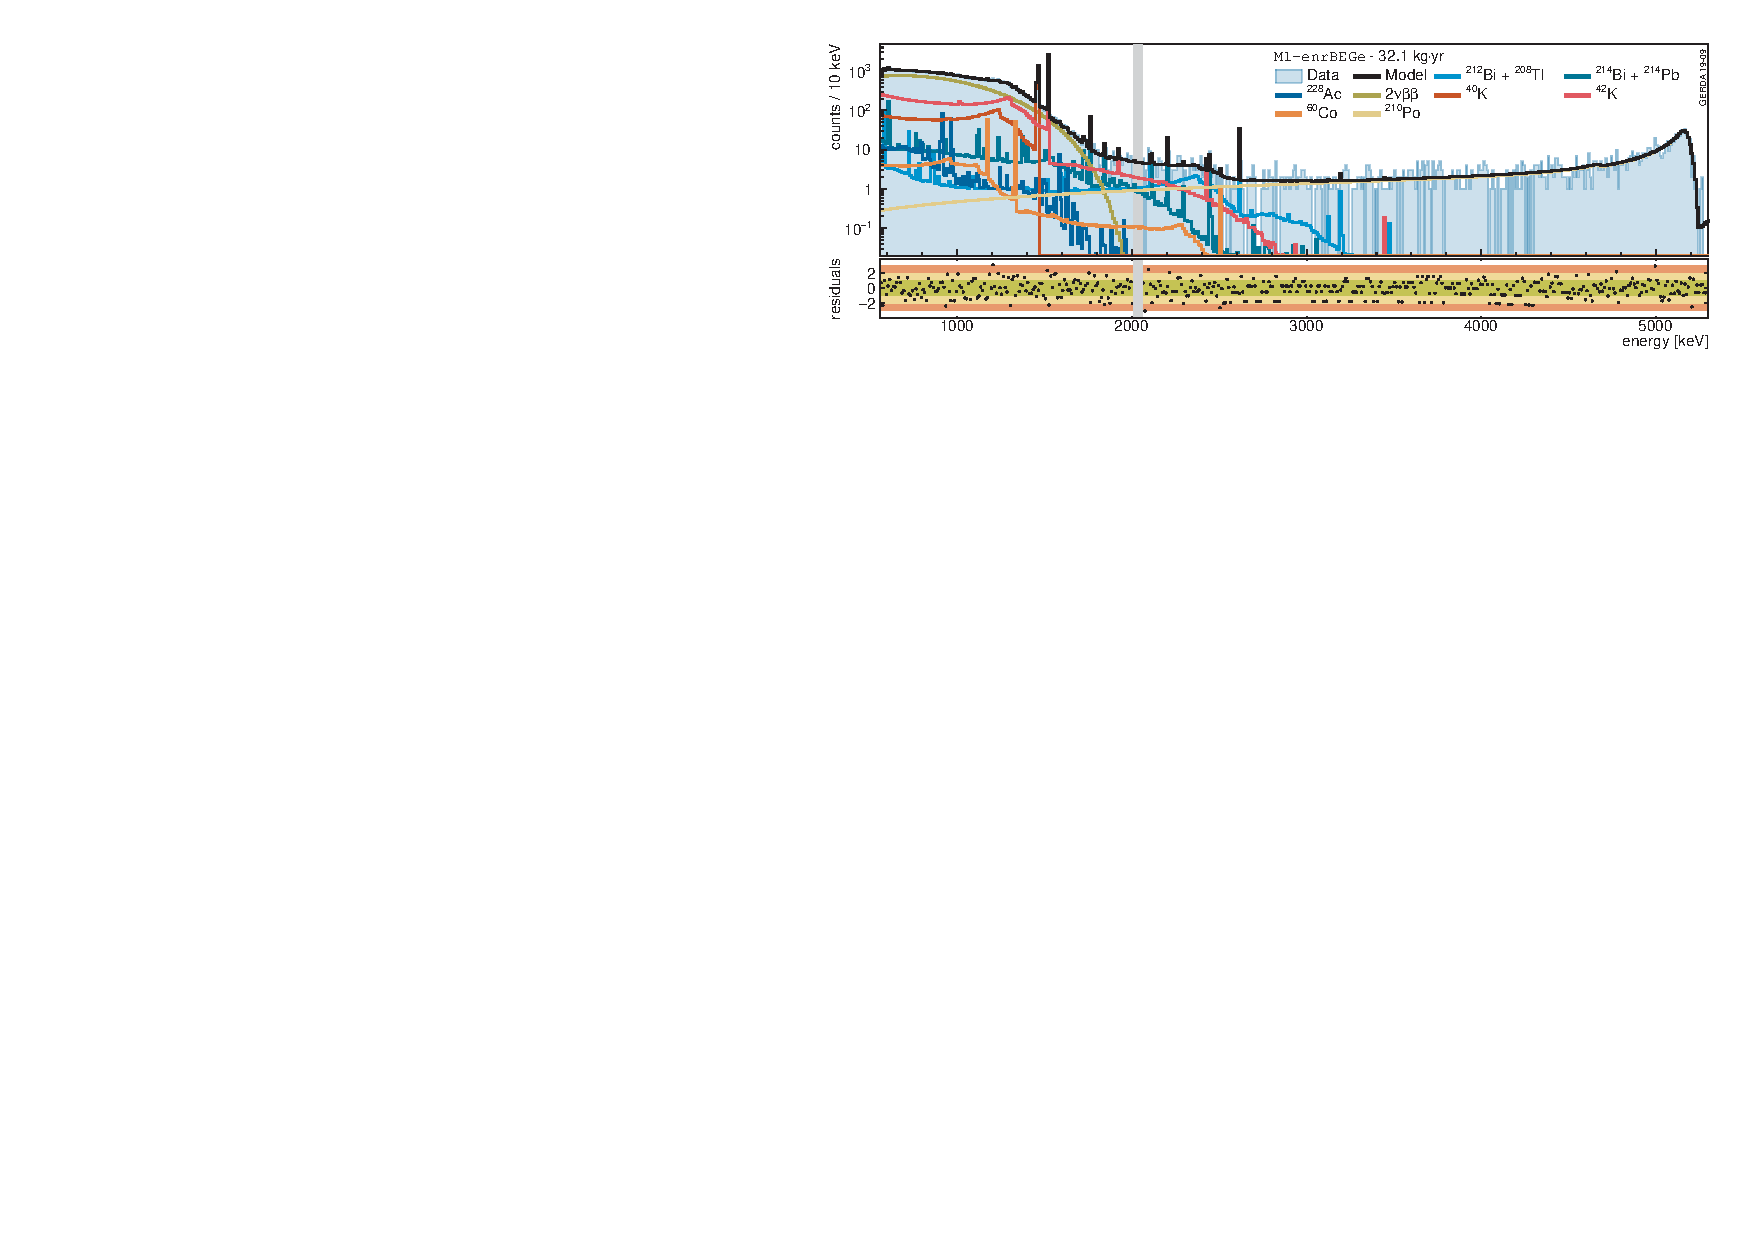
\includegraphics[width=\textwidth]{plots/bkg/raw/ph2/results/gmodel/gmodel-enrBEGe.pdf}
  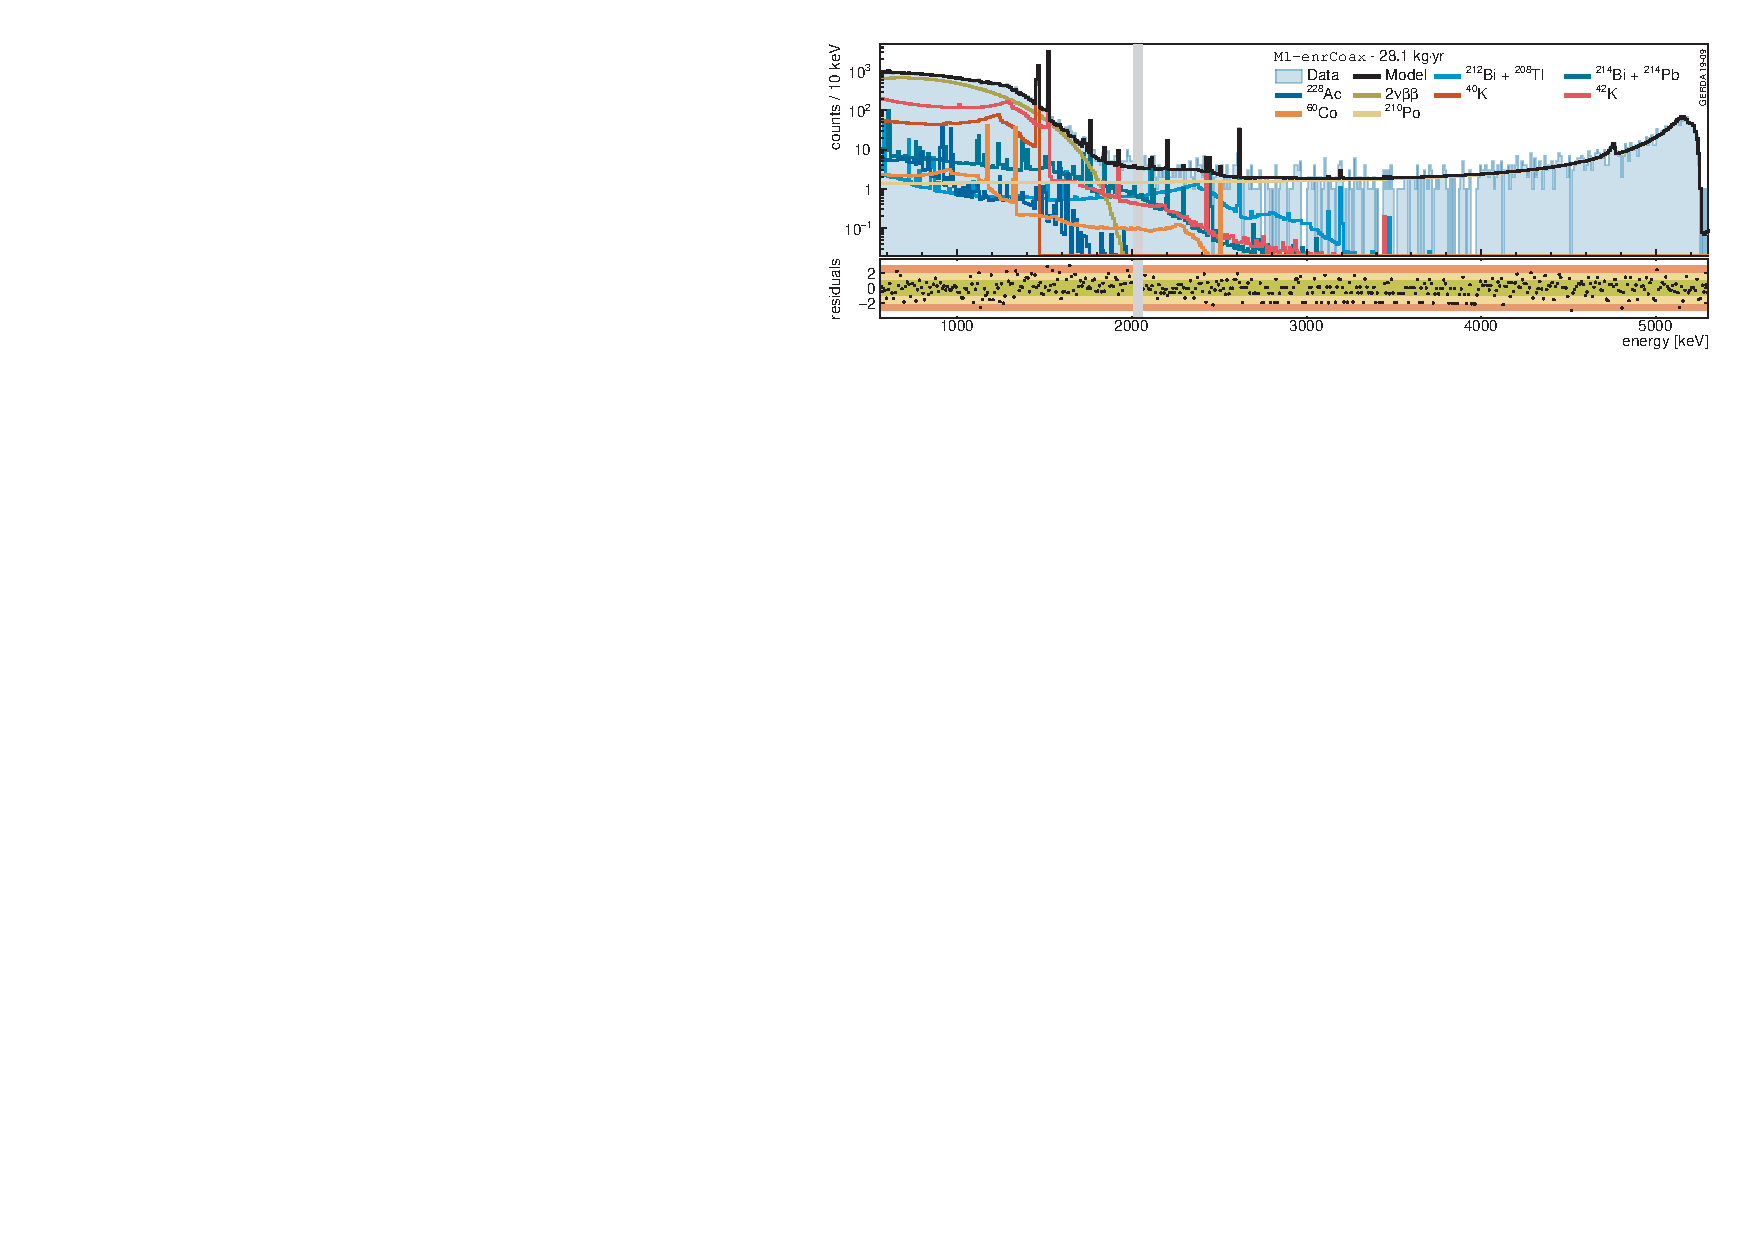
\includegraphics[width=\textwidth]{plots/bkg/raw/ph2/results/gmodel/gmodel-enrCoax.pdf}
  \includegraphics[width=\textwidth]{plots/bkg/raw/ph2/results/gmodel/gmodel-E1plusE2.pdf}
  \caption{%
    Background decomposition of the event energy distributions of the (from top to bottom)
    \enrBEGeII, \enrCoaxII\ and \enrGeII\ data sets.  Components referring to the same
    background source in different locations are summed together for visualization
    convenience. The blinded region $\qbbM \pm 25$~keV is highlighted in gray. In the
    three lower panels displaying the normalized residual distributions the central
    1$\sigma$-, 2$\sigma$- and 3$\sigma$-bands are marked in green, yellow and red,
    respectively. Note that for bins with low expected statistics due to the discrete
    nature of the measured spectrum not all colored bands are
    meaningful~\cite{Aggarwal2011}.%
  }\label{fig:bkg:raw:ph2:gmodel:results}
\end{figure}

\blocktitle{potassium}
The \kvz\ distribution is optimized to best fit the data. In order to disentangle the
\kvz\ \g\  and \b\ components, the volume inside and outside of the mini-shrouds is
separated in the pdf construction. Inside the mini-shrouds a homogeneous distribution is
compatible with the data as well as \kvz\ attached to the detectors contact surfaces. In
the fit model given here, a possible scenario is chosen where all \kvz\ is located on the
\nplus\ surfaces. However, we note that \kvz\ on the \pplus\ appears to partly substitute
the energy-degraded \a\ component in the \enrCoaxII\ data set if introduced in the fit and
predicts a higher total background index around \qbb. The extracted \kvz\ activity on the
\scoax\ \pplus\ contact in this case is $22\pm4$~\mubq\ corresponding to a
contribution to the background index around \qbb\ of $(7\pm1)\cdot10^{-3}~$\ctsper. For the \enrBEGeII\
data set the posterior distribution of a possible \kvz\ component on the \pplus\ contact
is compatible with zero. Outside the mini-shrouds an inhomogeneous distribution of the
\kvz\ decays better explains the observations. Detectors which are located at higher
positions in the strings show an excess of events in the \kvz\ 1525~keV \g\ line which is
compatible with a surplus of \kvz\ located right above the detector array (see
\cref{sec:bkg:raw:ph2:kmodel}). The full-range fit model contains a homogeneous \kvz\
distribution in LAr, outside the mini-shrouds, which is reconstructed with a specific
activity of $186\pm39$~\mubq/kg plus an additional distribution in the vicinity of the
cables (in LAr, above the array).
\newpar
A large fraction of the contamination with \kvn\ in the setup cannot be accounted for by
the screened hardware listed in \cref{tab:bkg:raw:ph2:gmodel:results}. We thus add a close
($\sim$1~cm) and a far ($\sim$50~cm) \kvn\ component with respect to the detector array
which are in fact replica of the pdfs for the mini-shrouds and the Tetratex\reg-coated copper
shrouds. These additional components absorb the excess indicated by the fit, the largest
part of the reconstructed events in the spectra is attributed to impurities close to the
array.
\newpar
The \kvn\ and \kvz\ distributions can be further split into smaller volumes and studied as
an extension of the potassium-tracking analysis (as described in
\cref{sec:bkg:raw:ph2:kmodel}) projected in detector space. The additional \kvn\ component
close to the array and the \kvz\ component above the array are split into 7 sub-components
on a string-by-string basis. The potassium concentration is in general found to be
asymmetric among the detector strings. In particular, a more prominent \kvz\ concentration
is found above the central string. This is consistent with the electrostatic drift of
\kvz\ ions induced by the electric field in the LAr which is generated by the unshielded
high-voltage flat cables biased with about 4~kV. The \kvn\ and \kvz\ spatial analysis
fitting the potassium \g\ lines projected in detector space is presented in full detail in
\cref{sec:bkg:raw:ph2:kmodel}.

\blocktitle{\a\ events}
The \a\ distribution is adjusted to best fit the data. The \Po\ peak at 5.2~MeV is found
to be best described by a mixture of pdfs obtained assuming different \pplus\ contact
thicknesses confirming results of the \phaseone\ background analysis~\cite{Agostini2013a}.
The empirical linear model which is used to describe \a\ events with degraded energy (see
\cref{sec:bkg:raw:ph2:amodel}), extends down to \qbb\ and below. For the \enrBEGeII\ data
set \a\ events are efficiently isolated using pulse shape discrimination (PSD) techniques
(see \cref{sec:gerda:cuts}).  All details about the \a\ events analysis can be found in
\cref{sec:bkg:raw:ph2:amodel}.

\blocktitle{\nnbb}
Most counts in the fit range are attributed to the \nnbb\ decay of \gesix; in fact its
continuous distribution dominates the spectrum up to almost 1.9~MeV. Here, the \nnbb\
half-life estimate is based on the \enrBEGeII\ data set only. An additional parameter,
$\delta^{2\nu}$, parametrizes the observed discrepancy to the value solely derived from
the \enrCoaxII\ data set. The value of $\delta^{2\nu}$ extracted from the fit amounts to a
surplus of 5\% of \nnbb\ counts observed in \enrCoaxII.  It mainly quantifies the
systematic biases between the active volume determination methods of the two detector
types. The \bege\ detectors active volume measurements are affected by a smaller
systematic uncertainty than the \scoax\ detectors~\cite{Agostini2013a, Agostini2019}.
Hence, the extracted \nnbb\ half-life, based on the \enrBEGeII\ data set and given here
only with statistical uncertainties, amounts to $\thalftwoM = (2.03 \pm 0.02) \cdot
10^{21}$~yr. A detailed discussion of this result follows in
\cref{sec:bkg:raw:ph2:discussion}.

\blocktitle{other}
Smaller contributions to the background model in the full energy range are attributed to
\Pbh\ and \Bih\ from the \Uh\ decay chain, \Ac, \Bil\ and \Tl\ from the \Thh\ decay chains
and \Co. With a total contribution in the fit range of $10^{-3}$~cts/keV for both the
\enrBEGeII\ and \enrCoaxII\ data set, \Pa\ gives negligible contribution to the spectra and
is therefore dropped from the full-range fit model. The central values preferred in the
full-range fit are driven by screening measurements and the spectral contributions are all
fully accounted for by the listed hardware components. The only exception is \Pbh\ and
\Bih\ where a minor contribution is added on the p$^+$ contact expected from the
observation of \a\ events belonging to the \Ra\ decay chain.

\begin{figure}
  \centering
  \includegraphics[width=0.45\linewidth]{plots/bkg/raw/ph2/results/gmodel/gmodel-roi-enrBEGe.pdf}
  \hspace{12pt}
  \includegraphics[width=0.45\linewidth]{plots/bkg/raw/ph2/results/gmodel/gmodel-roi-enrCoax.pdf}
  \caption{%
    Background decomposition for the \enrBEGeII\ (left) and the \enrCoaxII\ (right) data
    sets in the background window between 1930~keV and 2190~keV after data unblinding. The
    previously blinded window ($\qbbM \pm 25$~keV) is indicated by two dashed lines.  The
    background distribution before active background suppression in the \onbb\ analysis
    window can be well approximated with a constant function. For color code see
    \cref{fig:bkg:raw:ph2:gmodel:results}.%
  }\label{fig:bkg:raw:ph2:gmodel:results:roi}
\end{figure}

\blocktitle{background \\ at \qbb}
The background model describes the individual contributions to the total background index
around \qbb\ prior active background suppression (see
\cref{fig:bkg:raw:ph2:gmodel:results:roi}).  The background index is defined as the number
of counts over exposure and energy in the energy window from 1930~keV to 2190~keV
excluding the region around \qbb\ ($\qbbM \pm 5$~keV) and the intervals $2104 \pm 5$~keV
and $2119 \pm 5$~keV, which correspond to known \g\ lines from \Tl\ and \Bih. The values
for each background contribution are given in \cref{tab:bkg:raw:ph2:gmodel:results} and
are displayed as a fraction of the total background index in the following.
\begin{center}
  \includegraphics{plots/bkg/raw/ph2/results/gmodel/BI-bar.pdf}
\end{center}
The dominating background contribution around \qbb\ in the \enrBEGeII\ data set come from
\kvz. Isotopes from the \Thh\ decay chain, \a\ particles mainly with degraded energy and
isotopes from the \Uh\ decay chain contribute about equally. The estimated total
background indices extracted from the marginalized posterior distributions are
$\stat{16.04^{+0.78}_{-0.85}} \cdot 10^{-3}$~\ctsper\ for the \enrBEGeII\ data set and
$\stat{14.68^{+0.47}_{-0.52}} \cdot 10^{-3}$~\ctsper\ for the \enrCoaxII\ data set.

\section{Discussion}%
\label{sec:bkg:raw:ph2:discussion}

In general, the marginalized posterior distributions and the results of the material assay
measurements are in very good agreement. The only exception is constituted by the \kvn\
activity, which cannot be explained by the available prior information and is fit with the
additionally introduced components far and close to the detector array. The \kvz\ and
\a-event distributions, as already mentioned, cannot be constrained by screening
measurements and are adjusted to best fit the data.  The background model is not
completely free of parameter correlations. As shown in \cref{fig:bkg:raw:ph2:pdfs:gmodel}
several pdfs of the same source of background located in different structural components
are very similar and thus generate correlations. Most of them have been resolved by
introducing prior distributions based on the screening measurements.  However, a few
anti-correlations persist which are listed in \cref{tab:bkg:raw:ph2:corr}.

\begin{table}
  \centering
  \caption{%
    Correlations between fit components relative to the same background contamination in
    different locations.
  }\label{tab:bkg:raw:ph2:corr}
  \begin{tabular}{rllc}
    \toprule
    contamination & location 1                  & location 2         & correlation \\
    \midrule
    \Bih\ + \Pbh\ & mini-shrouds                & flat cables        & -0.43 \\
    % \midrule
    \mr{2}{\kvn}  & cabling                     & detector holders   & -0.45 \\
                  & cabling                     & close to the array & -0.63 \\
    % \midrule
    \mr{2}{\kvz}  & LAr -- outside mini-shrouds & \nplus\ contact    & -0.42 \\
                  & LAr -- outside mini-shrouds & LAr -- above array & -0.56 \\
    \bottomrule
  \end{tabular}
\end{table}

\blocktitle{\kvz}
For what concerns \kvz\ in the LAr volume outside the mini-shrouds, the adoption of an
additional pdf for \kvz\ above the detector array is purely motivated by the empirical
observation of an excess of background events in the top detectors. The prior knowledge is
indeed limited by the fact that the \kvz\ ions undergo drift due to the electrical fields
surrounding the detectors and high-voltage cables. Also, due to thermal gradients they can
be displaced by convection. With that considered, the presence of unshielded high-voltage
cables above the detector array can perhaps explain the excess of \kvz\ observed in this
region. A more detailed investigation of the \kvz\ distribution in LAr is not pursued any
further, as the full-range fit is inevitably not sensitive to such effects. A more
sophisticated Monte Carlo model would in fact not significantly impact the \kvz\ pdfs
shape. Nevertheless, some considerations are presented in the contest of the
potassium-tracking analysis, which is the only analysis presented here that could shed
some light on the problem (see \cref{sec:bkg:raw:ph2:kmodel}). Systematic uncertainties on
the \kvz\ pdf shape can also arise from the model of the partially-active dead layer of
the germanium detectors, which is treated as completely dead (the charge-collection
efficiency is set to zero throughout all the region between the surface and the full
charge-collection depth) in this analysis. The \b\ component of the \kvz\ spectrum above
the 1525~keV peak, relevant the in \onbb\ ROI, is indeed particularly affected by the
transition-layer model. It follows that the level of background model contributions from
\kvz\ sources particularly close to the \nplus\ contact might drastically change when
considering different active-volume models.

\blocktitle{background \\ window}
For each source of background the contribution to the background index at \qbb\ prior to
active background reduction is listed in \cref{tab:bkg:raw:ph2:gmodel:results}. The
statistical uncertainties on the single contributions to the background index are
generally of the order of 10\% or lower, with the exception of \kvz\ and energy-degraded
\a\ events, for which the uncertainty is roughly doubled. The two contributions are
affected by a higher uncertainty because they are not bound by screening measurements. In
particular, it has been argued how the \kvz\ content in the ROI, arising from \b\
particles reaching the detector active volume, might be strongly affected by the model of
the transition region. Because of the amount of systematic effects which might play a
significant role in the background decomposition of the ROI, the background indices
reported in \cref{tab:bkg:raw:ph2:gmodel:results} should be taken with a grain of salt.
\newpar
The background event distribution in the \onbb\ analysis window can be well approximated
with a constant function (see \cref{fig:bkg:raw:ph2:gmodel:results:roi}).  With this
assumption, the background indices extracted from data are $16.4^{+1.7}_{-1.6} \cdot
10^{-3}$~\ctsper\ for \enrBEGeII\ and $15.4^{+1.8}_{-1.6} \cdot 10^{-3}$~\ctsper\ for the
\enrCoaxII\ data set.  These values agree well with the background model description
presented in \cref{sec:bkg:raw:ph2:gmodel}. The background indices prior to further
analysis cuts and before the upgrade of the \gerda\ experiment to \phasetwo\ can be found
in reference~\cite{Agostini2013c}. For the \enrCoaxII\ data set the background index prior
to the upgrade of $(18 \pm 2) \cdot 10^{-3}$~\ctsper\ is very consistent with the values
presented here.  The background index of the \enrBEGeII\ data set instead is substantially
improved from a \phaseone\ value of $42^{+10}_{-8} \cdot 10^{-3}$~\ctsper\ to a value
which is at least $2.5\times$ smaller in \phasetwo\ despite a significant increase of
inactive hardware mass.\footnote{%
  Note the slight difference of the \enrBEGeII\ analysis data set presented here and the
  data set used for \onbb\ analysis for which the improvement in the background index is
  slightly higher ($3\times$ better background index). This is due to discarded \bege\
  data for which no PSD can be applied.
} Contributions to the background index from all isotopes have been improved with
respect to \phaseone\ with the exception of background introduced by \a\ surface events.
The most drastic improvement is notable for \kvz\ for which the background index
contribution for the \bege\ detectors appears four times smaller than before the upgrade
to \phasetwo.

\blocktitle{\nnbb\ \\ systematics}
As mentioned in \cref{sec:bkg:raw:ph2:gmodel}, the extracted \nnbb\ half-life estimate is
based on the \enrBEGeII\ data set only. The additional parameter $\delta^{2\nu}$ mainly
quantifies the systematic biases between the active volume determination methods of the
two detector types. The full charge collection depth (FCCD), which determines the active
volume of a detector, has been studied extensively in a detector characterization campaign for
the \bege\ detectors~\cite{Agostini2015e, Agostini2019}. The estimate of the FCCD used in
this analysis is based on measurements using an \Am\ source with characteristic \g\ lines
at 60~keV, 99~keV and 103~keV.  However, the FCCD was also measured using a \Co\ source
with characteristic \g\ energies of 1173~keV and 1332~keV. The latter FCCD$_\text{Co}$ is
systematically higher (about 3\%) with respect to the FCCD$_\text{Am}$. The discrepancy
could be explained by an energy dependence of the initial charge-carrier cloud size inside
the detector but the actual impact on the active volume is still under investigation. For
the \scoax\ detectors only FCCD values determined with a \Co\ source are available.
Another possible explanation for the observed shift might lie in the correction
which is applied to the \bege\ FCCD values consequently to the 2--3 year period they were
stored at room temperature, after being characterized and before being deployed into
liquid argon~\cite{Agostini2019}. The dead-layer growth effect in germanium detector has
never been rigorously studied, and therefore the applied correction might be biased. These
systematic uncertainties affecting the active volume estimates are investigated in
\cref{apdx:gedetav}.
Considering the systematic uncertainties affecting the determined active \gesix\ exposures
of the \enrBEGeII\ and \enrCoaxII\ data sets (1.8\% and 5\% respectively, see
\cref{tab:bkg:raw:ph2:datasets}), however, $\delta^{2\nu}$ is compatible with zero within
$1\sigma$.\footnote{%
  The systematic bias between the active volume estimates for the \bege\ and \scoax\
  detector types is a sub-dominant contribution in the \onbb\ analysis with respect to
  e.g.~PSD uncertainties.
}
\newpar
Various systematic effects have to be considered when estimating the uncertainty on the
\nnbb\ half-life \thalftwo. Due to the fact that the aim of this analysis is not a precise
\nnbb\ half-life measurement, for most of them only a conservative evaluation is provided.
Several systematic uncertainties arise from the Monte Carlo simulation framework.
Uncertainties due to the \geant\ model of particle interactions and propagation were
estimated to be of the order of 2\% in previous publications~\cite{Agostini2013a,
Agostini2015a}. Approximations in the implementation of the \gerda\ setup are
conservatively estimated within a $1-2$\% uncertainty range. This accounts for possible
spectral shape modifications due to inaccurate charge collection model between the \nplus\
contact layer and the active detector volume. Uncertainties induced by the theoretical
model of \nnbb\ decays implemented in \decayzero, as well as data acquisition and
selection methods are considered negligible. A 1.8\% contribution accounts for
uncertainties in the enrichment and active mass fraction determination (see active \gesix\
exposure in \cref{tab:bkg:raw:ph2:datasets}). All the systematic effects considered above
sum up to a total systematic uncertainty on \thalftwo\ of 3--4\%. In total this leads to
$T^{2\nu}_{1/2} = (2.03 \pm 0.09) \cdot 10^{21}$~yr compatible with earlier results
\cite{Agostini2013a, Agostini2015a}. A precision measurement of \thalftwo\ after the LAr
veto cut, which removes a large fraction of the background, will be presented in
\cref{chap:2nbb-ana} together with a careful estimation of the contribution of systematic
uncertainty sources.

\section{Full \phasetwo\ data analysis}%
\label{sec:bkg:raw:ph2p}

The background model presented in the past sections is based on data from the first part
of \phasetwo, for a total exposure of \gexpophasetwobkg. In April 2018 the data taking was
stopped to permit a hardware upgrade, in which five new detectors of the inverted-coaxial
type were deployed together with an improved LAr veto system. For further details about
the upgrade the reader is referred to \cref{sec:gerda:setup}. The data taking resumed in
May 2018 and ended in November 2019 after collecting \gexpophasetwopbkg\ of data valid for
the background model. In the following, the extension of the full-range energy spectrum
analysis to this data set is presented.

\blocktitle{data \\ and pdfs}
The total \gexpophasetwopbkg\ of single-detector data is divided according to the detector
type, giving three \Mone\ datasets: \enrBEGeIIp, \enrSCoaxIIp\ and \enrICoaxIIp.
Two-detector events are grouped in a single data set: \enrGeIIp. As above, their energy is
defined as the sum of the energies reconstructed in the two detectors. The four data sets,
their exposures and corresponding detector masses are listed in
\cref{tab:bkg:raw:ph2p:datasets}. The
energy spectra of the four data sets are shown in \cref{fig:bkg:raw:ph2p:data-desc}. In
addition to the list of background contributions in \cref{sec:bkg:raw:ph2:data} that can
be identified by eye in the spectra, an event excess is observed at 1124~keV in
\enrICoaxIIp\ which is attributed to the decay of \Zn\ in the germanium\footnote{%
  The \Zn\ present in the \icoax\ crystals is due to the reaction \nuc{Ge}{70}(n,
  \a{}2n)\Zn, induced by cosmic rays. It disintegrates mainly by electron capture to the
  1115~keV excited level of \nuc{Cu}{65} with a half-life of 244~days. \icoax\ detectors
  have been deployed in \gerda\ short after being produced, so the 1124~keV line (\g\
  de-excitation of \nuc{Cu}{65} coincident with K-shell X-rays) can be seen. A first
  reference to this decay in germanium has been found in a publication from the
  \textsc{Milano} \onbb\ experiment~\cite{Bellotti1986}.
}.
\newpar
The new experimental setup has been implemented into \mage. The changes to the software
include the implementation of the new \icoax\ detector geometry, the central fiber shroud
(see also \cref{fig:setup:magevolumes}, \emph{(c)} and \emph{(d)}) the new detector
arrangement (each holder unit supports only one detector) and the adaption of the
mini-shroud geometry. The updated \mage\ version is then used to run simulations of
background and signal contaminations and produce the corresponding pdfs, as described in
\cref{apdx:magepdfs}.

\begin{figure}
  \centering
  \includegraphics{plots/bkg/raw/ph2p/data-desc.pdf}
  \caption{%
    The \phasetwop\ data before analysis cuts.
  }\label{fig:bkg:raw:ph2p:data-desc}
\end{figure}

\begin{table}
  \centering
  \caption{%
    Properties of the data sets considered in this analysis. Further details about the
    \gerda\ detectors can be found in past publications~\cite{Agostini2013a,
    Agostini2018a, Miloradovic2020}. Note that the exposures for the \bege\ and \icoax\
    data sets are higher than those reported for the \onbb\ analysis~\cite{Kermaidic2020,
    Agostini2021}, because of additional data that that was discarded due to poor PSD
    detector performance. \fillme{check these numbers carefully}
  }\label{tab:bkg:raw:ph2p:datasets}
  \small
  \begin{tabular}{lccccc}
  \toprule
  \mr{2}{data set} & \mr{2}{composition}     & total Ge           & active \gesix\   & total Ge           & active \gesix\     \\
                   &                         & mass (kg)          & mass (kg)        & exposure (\kgyr)   & exposure (\kgyr)   \\
  \midrule
  \enrBEGeIIp\     & 29 \bege\footnotemark{} & $19.362 \pm 0.005$ & $17.17 \pm 0.32$ & $22.181 \pm 0.006$ & $17.31  \pm 0.32$  \\
  \enrSCoaxIIp\    & 6 \scoax\               & $11.827 \pm 0.002$ & $10.38 \pm 0.42$ & $13.179 \pm 0.003$ & $10.00  \pm 0.42$  \\
  \enrICoaxIIp\    & 4 \icoax\               & $ 7.802 \pm 0.002$ & $ 7.23 \pm 0.03$ & $ 8.775 \pm 0.002$ & $ 7.13  \pm 0.03$  \\
  \enrGeIIp\       & all enriched            & $38.991 \pm 0.006$ & $34.78 \pm 0.53$ & $44.135 \pm 0.007$ & $34.44  \pm 0.53$  \\
  \bottomrule
\end{tabular}

% vim: nowrap

\end{table}%
\footnotetext{%
  The \bege\ detector \GD{02D} is the only detector that does not fully
  deplete~\cite{Agostini2018a}. Hence, events triggered by this detector are not
  considered in either data set and it is omitted from the mass computation.
}

\blocktitle{background \\ expectations}
Because of the hardware changes, the expectations about the radio-purity of
the setup parts are different than before. In particular, the contribution of the signal
and high-voltage cables to the global background budget is expected to be lower, as
screening measurements show that the Tecnomec 3 mil cable type is cleaner. Moreover, the
introduction of material around the central string might increase the background level.
Many of the results of the first screening measurement campaign can be still used as prior
information for the \phasetwop\ background model, and part of the new material was
screened before installment in \gerda. The situation is summarized in \cref{apdx:assay}.

\blocktitle{analysis}
The full-range analysis of the binned energy spectra has been repeated for the \phasetwop\
data sets. The usual Poissonian likelihood that runs over each single energy bin and each
data set is maximized in a Bayesian setting. The C++ BAT-based~\cite{Caldwell2008}
software routine is publicly available on GitHub\footnote{\label{footnote:gerda-fitter}%
  The \texttt{gerda-fitter} software, available at
  \url{https://github.com/gipert/gerda-fitter}, is a Bayesian histogram fitting program
  written in C++ and based on the BAT toolkit. It is specialized and tested on the \gerda\
  data and pdfs format, but any ROOT histogram can be provided as input. The analysis is
  fully configurable in JSON format (\url{https://www.json.org}) and does not require
  writing or compiling C++ code (as one would need to do if using BAT directly). The list
  of features include: customization of nearly all the BAT parameters, computation of the
  Bayesian evidence, \pvalue\ computation, prior distribution configuration by
  analytical expression or external histogram, variable re-binning and posterior sampling of
  user-defined observables.
}. Variable bin sizes are used to represent data and pdfs in the analysis, to speed up the
computation. Dedicated, thin bins (depending on the energy resolution) are used for known
\g\ lines; larger ones (depending on the event rate) for the continuum. The analysis is
repeated with fixed-size bins (5~keV) to verify the consistency of the results.
\newpar
Given the lower \a-event rate compared to the first part of \phasetwo, the \a-events
analysis has not been repeated. In principle, the \Po\ contamination could have changed
after being manipulated during the upgrade works (see \cref{apdx:timealpha}), resulting in
a different shape of the event energy distribution. To avoid using a wrong model of \a\
events in the full-range fit, only two large bins are used in the high-energy region of
the single-detector event spectra: $[2620, 4500]$~keV and $[4500, 5260]$~keV. In this way,
no potential bias is introduced, and this last part of the energy range is just used to
constrain the \a\ event contribution in the \nnbb\ region. The \enrBEGeII\ and \enrCoaxII\
\a-model pdfs (see \cref{sec:bkg:raw:ph2:amodel}) are re-used for \enrBEGeIIp\ and
\enrSCoaxIIp, respectively. The \enrBEGeII\ pdf is also arbitrarily used for \enrICoaxIIp,
since the corresponding detectors have been introduced in \phasetwop\ for the first time.
The faithfulness of the pdfs is verified \emph{a posteriori}.
\newpar
Since also the potassium-tracking analysis has not been repeated, no prior information is
used to constrain the potassium activity. Priors are extracted from screening
measurements results: Gaussian distributions for positive contamination detections and
exponential distributions of the form $e^{-2.3 \mu x}$ for 90\% C.L.~upper limits.

\blocktitle{results}
A first fit model is constructed including all the background components for which a prior
distribution is available from material screening measurements. Additionally, based on the
results for the first data of \phasetwo, two unconstrained \kvn\ fit
components are added --- one \emph{close}, on the mini-shrouds and \emph{far}, on the
outer fiber shroud. As done before, 6 pdfs for \kvz\ are considered: one corresponding to
a homogeneous distribution in the LAr volume enclosed by the mini-shrouds, one outside and
one in a cylinder above the array (see \cref{apdx:magepdfs} and
\cref{sec:bkg:raw:ph2:gmodel}). The other three pdfs correspond to \kvz\ homogeneously
distributed on the \nplus\ surface of the detectors included in the three \Mone\ data
sets. A linear function $b_1+b_2x$ is also included for each \Mone\ data set
separately (6 parameters in total) to account for energy-degraded \a\ events, as also
done in \cref{sec:bkg:raw:ph2:gmodel}. Given the known discrepancies between the detector
active volume determination methods, three independent parameters are used for the
\nnbb-decay half-lives reconstructed from the three \Mone\ data sets. A uniform prior is
set on $1/\thalftwoM$\footnote{%
  The detailed fit configuration file is available at
  \url{https://github.com/gipert/gerda-fitter/config/phaseIIplus/gerda-fitter-phIIp-raw-global_extra_blocks.json}.
}.
\newpar
The resulting background decomposition of the four analysis data sets is shown in
\cref{fig:bkg:raw:ph2p:results-1,fig:bkg:raw:ph2p:results-2,fig:bkg:raw:ph2p:results-3}.
Data is presented with the variable binning used in the analysis and a fixed-width 15~keV
binning. In this rich configuration, most of the marginalized posteriors are driven by
their respective prior distribution. This is expected, given the known correlations
between the pdfs and the low count rate of some background sources. All the marginalized
posteriors are compatible with the prior information. The additional, special, \kvn\
component close to the detector array still reports a non-zero result, while the posterior
for \kvn\ far from the array is peaked at zero.  Differently from what has been previously
obtained in \cref{sec:bkg:raw:ph2:gmodel}, the \kvz\ component on the \nplus\ contact of
the \bege\ detectors is now compatible with zero. This is due to the non-null \bege\
detectors transition layer model used to obtain the corresponding pdf, which increases the
rate of \b\ events above the 1525~keV peak (c.f.r.~\cref{fig:bkg:raw:ph2:pdfs:gmodel:K42})
and decreases the compatibility with experimental data.

\begin{sidewaystable}
  \centering
  \footnotesize
  \caption{%
    Summary of the analysis parameter estimates. Global mode and marginalized mode, along
    with its smallest 68\% C.I., are reported as representatives of the posterior
    parameter distribution. The number of reconstructed counts in the fit range and the
    background index at \qbb\ prior active background suppression are listed for each
    component and each analysis data set. The original type of prior distribution is
    marked with \m{[f]} for flat, \m{[g]} for Gaussian and \m{[e]} for exponential.
    \fillme{fill BIs}
  }\label{tab:bkg:raw:ph2p:gmodel:results}
  \newcolumntype{H}{>{\setbox0=\hbox\bgroup}c<{\egroup}@{}}
\newcolumntype{x}[1]{>{\centering\arraybackslash}p{#1}}
\newcommand{\mrr}[2]{\multirow{#1}[1]{*}{#2}}
\newcommand{\mrc}[2]{\multirowcell{#1}{#2}}

\begin{tabular}{%
  r
  l
  c
  S[% global mode
    table-format=4.2,
    table-number-alignment=right,
    table-text-alignment=right,
    table-parse-only
  ]
  r@{ }l% marginalized with 68% CI interval
  S[% screening measurements
    table-number-alignment=left,
    table-text-alignment=left,
    table-parse-only
  ]
  S[% BEGe
    table-format=5.0,
    table-number-alignment=center,
    table-text-alignment=center,
    table-auto-round=true
  ]@{ | }
  l
  S[% Coax
    table-format=4.0,
    table-number-alignment=center,
    table-text-alignment=right,
    table-auto-round
    ]@{ | }
  l
  S[% M2-All
    table-format=4.0,
    table-number-alignment=center,
    table-text-alignment=center,
    table-auto-round
  ]
}
  \toprule
  \mrr{3}{source}      & \mrr{3}{\m{[prior]} location}         & \mrr{3}{units}      & {\mrc{3}{global\\mode}} & \mc{2}{\mrc{3}{marg.~mode\\with 68\% CI}} & {\mrr{3}{screening}} & \mc{5}{model content in fit range | BI at \qbb}                                             \\
                       &                                       &                     &                         &       &                                   &                      & \mc{5}{units: cts | $10^{-3}$\ctsper}                                                       \\
  \cmidrule(lr){8-12}
                       &                                       &                     &                         &       &                                   &                      & \mc{2}{\enrBEGeII}                     & \mc{2}{\enrCoaxII}                     & \enrGeII\ \\
  \midrule
  \mr{2}{\nnbb}        & \m{[f]} \bege\ detectors              & \mr{3}{$10^{21}$yr} &                         &       &                                   & {--}                 &         & \mrc{2}{0}                   &         & \mrc{2}{0}                   &           \\
                       & \m{[f]} \scoax\ detectors             &                     &                         &       &                                   & {--}                 &         & \mrc{2}{0}                   &         & \mrc{2}{0}                   &           \\
                       & \m{[f]} \icoax\ detectors             &                     &                         &       &                                   & {--}                 &         & \mrc{2}{0}                   &         & \mrc{2}{0}                   &           \\
  \midrule
  \mr{3}{\Bil\ + \Tl}  & \m{[e]} flat cables                   & \mr{3}{$\upmu$Bq}   &                         &       &                                   & < 410                &         & \mrc{3}{3.52\\$[3.30,3.76]$} &         & \mrc{3}{2.21\\$[2.03,2.34]$} &           \\
                       & \m{[g]} copper shrouds$^{\dagger}$    &                     &                         &       &                                   & 194 \pm 19           &         &                              &         &                              &           \\
                       & \m{[g]} mini-shrouds                  &                     &                         &       &                                   & 18  \pm 5            &         &                              &         &                              &           \\
  \midrule
  \mr{6}{\Pbh\ + \Bih} & \m{[f]} \pplus\ (BEGe)                & \mr{6}{$\upmu$Bq}   &                         &       &                                   & {--}                 &         & \mrc{6}{2.63\\$[2.50,2.78]$} &         & \mrc{6}{3.16\\$[2.83,3.50]$} &           \\
                       & \m{[f]} \pplus\ (Coax)                &                     &                         &       &                                   & {--}                 &         &                              &         &                              &           \\
                       & \m{[g]} flat cables                   &                     &                         &       &                                   & 660 \pm 210          &         &                              &         &                              &           \\
                       & \m{[g]} copper shrouds$^{\dagger}$    &                     &                         &       &                                   & 532 \pm 53           &         &                              &         &                              &           \\
                       & \m{[g]} mini-shrouds                  &                     &                         &       &                                   & 43  \pm 13           &         &                              &         &                              &           \\
                       & \m{[g]} SiPM-ring                     &                     &                         &       &                                   & 351 \pm 97           &         &                              &         &                              &           \\
  \midrule
  \mr{9}{\kvn}         & \m{[g]} flat cables                   & \mr{9}{mBq}         &                         &       &                                   & 6  \pm 2             &         & \mrc{9}{0}                   &         & \mrc{9}{0}                   &           \\
                       & \m{[g]} front-end electronics         &                     &                         &       &                                   & 13 \pm 4             &         &                              &         &                              &           \\
                       & \m{[g]} copper shrouds$^{\dagger}$    &                     &                         &       &                                   & 18 \pm 2             &         &                              &         &                              &           \\
                       & \m{[g]} fiber shroud                  &                     &                         &       &                                   & 2.9 \pm 0.6          &         &                              &         &                              &           \\
                       & \m{[g]} detector holders              &                     &                         &       &                                   & 2.8 \pm 0.6          &         &                              &         &                              &           \\
                       & \m{[g]} mini-shrouds                  &                     &                         &       &                                   & 1.7 \pm 0.6          &         &                              &         &                              &           \\
                       & \m{[g]} SiPM ring                     &                     &                         &       &                                   & 2 \pm 2              &         &                              &         &                              &           \\
                       & \m{[f]} far from the array            &                     &                         &       &                                   & {--}                 &         &                              &         &                              &           \\
                       & \m{[f]} close to the array            &                     &                         &       &                                   & {--}                 &         &                              &         &                              &           \\
  \midrule
  \mr{4}{\kvz}         & \m{[f]} \nplus\ (BEGe)                & \mr{2}{$\upmu$Bq}   &                         &       &                                   & {--}                 &         & \mrc{4}{5.69\\$[4.58,6.29]$} &         & \mrc{4}{1.29\\$[1.15,1.40]$} &           \\
                       & \m{[f]} \nplus\ (Coax)                &                     &                         &       &                                   & {--}                 &         &                              &         &                              &           \\
                       & \m{[f]} LAr {--} above array          & \mr{2}{Bq}          &                         &       &                                   & {--}                 &         &                              &         &                              &           \\
                       & \m{[f]} LAr {--} outside mini-shrouds &                     &                         &       &                                   & {--}                 &         &                              &         &                              &           \\
  \midrule
  \mr{3}{\Ac}          & \m{[g]} copper shrouds$^{\dagger}$    & \mr{4}{$\upmu$Bq}   &                         &       &                                   & 62 \pm 6             &         & \mrc{4}{0.36\\$[0.31,0.40]$} &         & \mrc{4}{0.33\\$[0.28,0.37]$} &           \\
                       & \m{[e]} detector holders              &                     &                         &       &                                   & < 250                &         &                              &         &                              &           \\
                       & \m{[g]} mini-shrouds                  &                     &                         &       &                                   & 18  \pm  5           &         &                              &         &                              &           \\
  \Co\                 & \m{[e]} flat cables                   &                     &                         &       &                                   & < 250                &         &                              &         &                              &           \\
  \midrule
  \mr{4}{\a\ decays}   & \m{[f]} \Po\ + \Ra\ chain (\bege)     & \mr{3}{cts}         &                         &       &                                   & {--}                 &         & \mrc{4}{3.31\\$[3.12,3.78]$} &         & \mrc{4}{4.76\\$[4.40,5.08]$} &           \\
                       & \m{[f]} \Po\ + \Ra\ chain (\scoax)    &                     &                         &       &                                   & {--}                 &         &                              &         &                              &           \\
                       & \m{[f]} \Po\ + \Ra\ chain (\icoax)    &                     &                         &       &                                   & {--}                 &         &                              &         &                              &           \\
  \bottomrule%
\end{tabular}%

% vim: nowrap
%
\end{sidewaystable}

\begin{figure}
  \centering
  \includegraphics[width=\textwidth]{plots/bkg/raw/ph2p/results/gmodel/enrBEGe-results.pdf}
  \includegraphics[width=\textwidth]{plots/bkg/raw/ph2p/results/gmodel/enrCoax-results.pdf}
  \includegraphics[width=\textwidth]{plots/bkg/raw/ph2p/results/gmodel/enrInvCoax-results.pdf}
  \caption{%
    The background decomposition of the last \gexpophasetwopbkg\ of \gerdatwo\ before
    analysis cuts. The binning is the one used in the analysis. Contributions from
    the same radioactive decay are summed for visualization purposes. The data-to-model
    ratio is shown in the bottom panels together with the smallest 60\%, 95\% and 99\%
    confidence intervals.
  }\label{fig:bkg:raw:ph2p:results-1}
\end{figure}

\begin{figure}
  \centering
  \includegraphics[width=\textwidth]{plots/bkg/raw/ph2p/results/gmodel/enrE1plusE2-results.pdf}
  \includegraphics[width=\textwidth]{plots/bkg/raw/ph2p/results/gmodel/enrBEGe-results-fixbw.pdf}
  \includegraphics[width=\textwidth]{plots/bkg/raw/ph2p/results/gmodel/enrCoax-results-fixbw.pdf}
  \caption{%
    The background decomposition of the last \gexpophasetwopbkg\ of \gerdatwo\ before
    analysis cuts. The binning is the one used in the analysis. Contributions from
    the same radioactive decay are summed for visualization purposes. The data-to-model
    ratio is shown in the bottom panels together with the smallest 60\%, 95\% and 99\%
    confidence intervals.
  }\label{fig:bkg:raw:ph2p:results-2}
\end{figure}

\begin{figure}
  \centering
  \includegraphics[width=\textwidth]{plots/bkg/raw/ph2p/results/gmodel/enrInvCoax-results-fixbw.pdf}
  \includegraphics[width=\textwidth]{plots/bkg/raw/ph2p/results/gmodel/enrE1plusE2-results-fixbw.pdf}
  \caption{%
    The background decomposition of the last \gexpophasetwopbkg\ of \gerdatwo\ before
    analysis cuts. The binning is the one used in the analysis. Contributions from
    the same radioactive decay are summed for visualization purposes. The data-to-model
    ratio is shown in the bottom panels together with the smallest 60\%, 95\% and 99\%
    confidence intervals.
  }\label{fig:bkg:raw:ph2p:results-3}
\end{figure}

\blocktitle{\thalftwo}
The three marginalized posteriors for the \nnbb-decay half-life, coming from the three
detector types separately, are shown in \cref{fig:bkg:raw:ph2p:gmodel:2nbb-post}. The
distributions have been obtained by re-sampling of the Markov chain\footnote{%
  Note that the priors on \thalftwo\ are not exactly flat, as the real uniform priors are
  set on the number of \nnbb\ counts, which is proportional to $1/\thalftwoM$. In this
  range of half-life values, however, they can be well approximated by a flat
  distribution.
}. As it is evident, a systematic discrepancy between the half-life predicted with \bege\
detectors and with \scoax\ detectors is found, at the same level of what observed in the
analysis of the \enrBEGeII\ and \enrCoaxII\ (c.f.r.~\cref{sec:bkg:raw:ph2:gmodel}). The
half-life predicted with \icoax\ detectors, on the other hand, seems to give the same
results extracted from the \scoax\ detectors. Again, there is a clear evidence for a
systematic underestimation of the \scoax\ and \icoax\ detector active volume, or
overestimation of the \bege\ detector active volume, or even a more complex effect. This
issue is addressed in detail in \cref{apdx:gedetav}, where additional evidence for the
presence of systematic biases in the active volume estimate is presented. As remarked
before, in the case of \bege\ detectors the shift could be largely due to uncertainties on
the \nplus\ dead-layer growth speed at room temperature.
\newpar
To further investigate the origin of the discrepancy, the full-range analysis is repeated
with pdfs (for all background sources and \nnbb-decay) that assume the preliminary active
and transition layer model extracted from \Arl\ data, which is described in detail in
\cref{sec:gedetav:ar39}. A comparison between the latter and the official model is given
in \cref{fig:gedetav:ar39-results}, and the obtained \thalftwo\ posteriors are shown in
\cref{fig:bkg:raw:ph2p:gmodel:2nbb-post-ar39av}. \icoax\ and \scoax\ posteriors are
shifted up, while the \bege\ posterior is shifted down, achieving a better compatibility
between the three estimates. These results, however, must be taken with a grain of salt:
the \Arl\ data analysis is still at an early stage and the impact of possible sources of
systematic uncertainties has not been evaluated yet. They demonstrate, indeed, the
potential of an analysis of \Arl\ data to obtain unbiased estimated of the detector active
volumes in their experimental working conditions. A robust estimated of the active volumes
is, in fact, of great interest for the \nnbb\ analysis and the \onbb\ search.

\begin{figure}
  \centering
  \includegraphics{plots/bkg/raw/ph2p/results/gmodel/2nbb-posteriors.pdf}
  \caption{%
    Marginalized posterior distributions of the \nnbb-decay half-lives reconstructed from
    the three \enrBEGeIIp, \enrSCoaxIIp\ and \enrICoaxIIp\ data sets separately. The three
    parameters are independent from each other in the fit and carry a nearly uniform prior
    distribution (the prior is actually uniform on $1/\thalftwoM$).
  }\label{fig:bkg:raw:ph2p:gmodel:2nbb-post}
\end{figure}

\begin{figure}
  \centering
  \includegraphics{plots/bkg/raw/ph2p/results/gmodel/2nbb-posteriors-ar39av.pdf}
  \caption{%
    Marginalized posterior distributions of the \nnbb-decay half-lives reconstructed from
    the three \enrBEGeIIp, \enrSCoaxIIp\ and \enrICoaxIIp\ data sets separately. The pdfs
    in the analysis have been computed with the preliminary detector active volume model
    results obtained from \Arl\ data in \cref{sec:gedetav:ar39}. The systematic shifts
    observed in \cref{fig:bkg:raw:ph2p:gmodel:2nbb-post} are reduced.
  }\label{fig:bkg:raw:ph2p:gmodel:2nbb-post-ar39av}
\end{figure}

\blocktitle{upgrade \\ effect}
To detect changes of the background level before and after the \phasetwop\ upgrade works,
the full-range analysis of the energy spectra presented in \cref{sec:bkg:raw:ph2:gmodel}
and in this section has been repeated with a minimal fit configuration. A representative
set of background components has been identically selected for the two analyses:
\nnbb-decay for each detector type, \Bil, \Tl, \Pbh, \Bih, and \Co\ on cables, \Ac\ on
detector holders, \kvn\ close (mini-shrouds) and far (outer fiber shroud) from the array,
\kvz\ in LAr outside/inside the mini-shrouds, above the array and on the \nplus\ surface
for each detector type, the \a\ model pdfs and \Zn\ in the \icoax\ detectors.
\newpar
In \cref{fig:bkg:raw:ph2p:comparison} the number of reconstructed counts above the \Arl\
Q-value (565~keV) for each radioactive source, for each single-detector event data set,
before and after the \phasetwop\ upgrade, in units of \gesix\ exposure is shown. The
extracted count rates before and after the upgrade are consistent within their statistical
error, except for \Th\ (\Bil\ and \Tl) and \Co\ contaminations, which seem to have
increased after the upgrade.

\begin{figure}
  \centering
  \includegraphics{plots/bkg/raw/ph2p/results/gmodel/ph2-comparison.pdf}
  \caption{%
    Comparison between the single-detector event background counts in units of \gesix\
    exposure above the \Arl\ Q-value (565~keV) reconstructed with the background model
    analysis before and after the \phasetwop\ hardware upgrade.
  }\label{fig:bkg:raw:ph2p:comparison}
\end{figure}

The results of the background decomposition of the full \gerdatwo\ data before the LAr
veto and PSD cuts have been combined in \cref{fig:bkg:raw:results}. The single-detector
data sets \enrBEGeII, \enrCoaxII, \enrBEGeIIp, \enrSCoaxIIp\ and \enrICoaxIIp\ have been
combined in the upper panel; \enrGeII\ and \enrGeIIp\ have been combined in the bottom
panel.

\begin{figure}
  \centering
  \includegraphics{plots/bkg/raw/combined-results.pdf}
  \caption{%
    Background decomposition of the full \gerdatwo\ data set, divided in single- and two-
    detector events. Background components are grouped per radioactive source for
    visualization purposes.
  }\label{fig:bkg:raw:results}
\end{figure}

\chapsummary
\begin{itemize}
  \item The development of a careful model of the background in the full energy range of
    events collected by a neutrinoless double-beta decay experiment is crucial in order to
    understand the composition of background events in the region of interest. The spatial
    distribution of the background sources and their effect in the data is useful
    information in designing future hardware upgrades or experimental efforts. Last but
    not least, a background model grants access to the two-neutrino double-beta decay
    event distribution, that can be analyzed to determine the half-life of the process and
    to constrain the presence of beyond the standard model physics phenomena.
  \item The energy spectrum of single- and two-detector events before the LAr veto and the
    PSD cuts, divided by detector type, is decomposed in a Bayesian setting, which
    includes prior information from material screening measurements. The expected
    distribution of the various background components is generated starting from a full
    Monte Carlo simulation chain of the experimental setup. The shape of high-energy events,
    attributed to \a\ decays on the \pplus\ detector contacts, is studied separately and
    incorporated in the final fit. The spatial information enclosed in potassium events
    from the two intense \g\ peaks is exploited in a potassium-tracking analysis, which
    considers data from each detector separately and is therefore able to better
    unravel the origin of the background events. The results are incorporated in the final
    fit as prior information.
  \item The obtained model describes the data and reproduces the screening measurement
    results to a satisfying degree of accuracy. An unexpected higher \kvn\ contamination
    is found both in locations close to the detector array and far from it. Moreover, an
    excess of \kvz\ events is seen by detectors at the top of the array, possibly
    attributed to the electromagnetic attraction of the potassium ions towards the
    high-voltage cables. The background at the \onbb\ is found to be flat except for two
    \g\ lines from \Tl\ and \Bih. The main contribution is \kvz\ \b\ particles, while \a\
    events and isotopes from the \Thh\ and \Uh\ decay chains contribute equally. However,
    the composition of the background at the \onbb\ Q-value must be taken with a grain of
    salt: many sources of systematic uncertainties have not been taken into account.
  \item A discrepancy between the \nnbb-decay half-life reconstructed with \bege\
    detectors and the one from \scoax\ detectors is found, revealing the presence of a
    systematic bias between the two active volume estimates. This is attributed to the
    employment of different measurement techniques or the underestimation of the \bege\
    detectors dead-layer growth at room temperature. Nevertheless, the two results are
    compatible within the systematic uncertainty attributed to the active volume
    estimates. The measurement of the \nnbb\ half-life is, however, out of the scope of
    the analysis of data before the analysis cuts. A more precise determination will be
    presented in \cref{chap:2nbb-ana}, based on data after LAr veto cut.
  \item The full-range analysis of the energy spectrum has been repeated for data
    collected after the \phasetwop\ upgrade. The experimental setup implemented in the
    Monte Carlo has been updated, and new pdfs have been generated. Compared to the first
    part of \phasetwo, the background has not significantly changed as a consequence of
    the upgrade works. A systematic shift between the \nnbb-decay half-life estimates from
    \scoax\ and \icoax\ detectors, from one side, and \bege\ detectors is also observed
    with the new data. A preliminary re-analysis using the detectors active volume
    extracted from \Arl\ data seems to remove this tension.
\end{itemize}

% vim: tw=90

  %!TEX root = ../main.tex

\chapter{The background after the LAr veto cut}\label{chap:bkg:lar:ph2}

All what has been shown until now concerns data before the LAr and PSD cut. In this
chapter a model of the background after the LAr veto cut will be presented, based on a
Monte Carlo simulation of the LAr scintillation light propagation. Being able to describe
the background after this major event selection is indeed of great interest to study the
distribution of two-neutrino double-beta decay events, which are almost never vetoed by
the LAr veto system. As extensively shown in \cref{chap:theory}, the presence of several
new physics phenomena can be constrained by looking at the shape of the \nnbb\ events
distribution. Understanding the action of the LAr veto cut on background events from the
point of view of the background model requires, however, a full Monte Carlo simulation of
the LAr scintillation mechanism as well as the implementation of all the relevant material
and surface optical properties that contribute to light propagation in the \gerda\ experimental
setup. Implementing such a simulation, as it will be shown, requires an accurate knowledge
of many optical parameters, which is not always the case, unfortunately, with the \gerda\
setup. Nevertheless, it is possible to use special calibration data with low-activity
sources and the LAr veto instrumentation turned on to constrain the LAr veto Monte Carlo
model. An independent analysis of this special data set is used to tune the unknown
optical parameters in the Monte Carlo such to reproduce the observed vetoing performance.
The obtained parameters are then used to produce a map of the LAr scintillation light
detection probability, which is applied to the background model simulations in order to
obtain the LAr veto flag. Based on these new background model pdfs, a statistical analysis
to test possible deviations of the \nnbb\ distribution from its Standard Model description
will be finally presented.
\newpar
The chapter is structured as follows: \fillme{fillme}

\section{Optical physics in \mage}%
\label{sec:bkg:lar:ph2:mage}

Optical materials and surfaces are implemented in \mage\ through the relevant \geant\
libraries. Once properties like reflectivity, wavelength-shifting capabilities,
attenuation lengths, scintillation yields etc.~are defined, the \geant\ core routines take
care of simulating light propagation accordingly. When defining optical parameters in the
Monte Carlo, one must keep in mind what are the typical photon wavelengths that come to
play in the \gerda\ setup. The most important wavelength is 128~nm, in the so-called
vacuum-ultra-violet (VUV) regime, which defines the energy of the photon emitted by the
LAr scintillation process. The second interesting regime is in the 400--600~nm range,
typical of photons which are wavelength-shifted (WLS) in the fiber curtain or by
Tetraphenil-Butadiene (TPB) coatings to match the absorption range of the light detectors
(PMTs, SiPMs). As it will be clear in the next sections, many optical parameters are
poorly known in the VUV regime or depend on the details of the experimental setup (LAr
purity, WLS coating thickness etc.), and a dedicated measurement should be therefore
performed.  In the following sections a reference list of the optical properties
implemented in \mage\ is provided, with references to the literature.

\blocktitle{liquid \\ argon}
Key properties of the liquid argon from the point of view of the vetoing performance in
\gerda\ are the scintillation mechanism, the refractive index and the attenuation length.
The first two are relatively well known, while the latter strongly depends on the LAr
purity, which has not been measured for \gerda. We recall here that the deployed LAr has
not been subject to any purification process, and is therefore expected to meet the purity
specifications of natural argon.

\begin{description}

  \item[Refractive index] Its implementation is dependent on the photon energy (shown in
    \cref{fig:bkg:lar:ph2:mage:lar-props}). Formulas are taken from~\cite{Bideau-Mehu1981}
    and give about 1.41 at 128~nm. A more recent measurement, similarly based on an
    extrapolation of measured data to lower wavelengths, suggests a lower value of about
    1.37~\cite{Babicz2018}.

  \item[Rayleigh scattering length]. Depends on the refractive index and therefore the
    photon energy (shown in \cref{fig:bkg:lar:ph2:mage:lar-props}). Formulas are taken
    from~\cite{Seidel2002}. The already implemented refractive index values are used. The
    obtained scattering length value at 128~nm is about 60~cm. The value suggested
    in~\cite{Babicz2018} is 91~cm, 50\% higher.

  \item[Scintillation spectrum] Taken from~\cite{Heindl2010}, which reports an
    experimental measurement (fig.~1 and 2). Only the (gaussian) peak is implemented in
    \mage, as the non-gaussian contributions are of several orders of magnitude lower and
    are therefore negligible. A normal distribution $(\mu=128\;\text{nm},
    \sigma=2.929\;\text{nm})$ is implemented (\cref{fig:bkg:lar:ph2:mage:lar-props}).

  \item[Scintillation yield] Different scintillation processes are defined in the \mage\
    physics list for different ionizing particles, that in general have different
    scintillation yields in LAr. A default, reference value of $51\;\upgamma/\text{keV}$
    is set for all particles~\cite{Doke2002}. This value does certainly not represent the
    reality of \gerda, as the yield strongly depends on the electric field configuration
    and the quencher impurities. Unfortunately a a reliable direct measure of the
    scintillation yield of the \gerda\ LAr is not available.  Indirect measurements were
    performed within the \LArGe\ setup~\cite{Lehnert2015} and with a dedicated setup
    deployed inside the \gerda\ cryostat~\cite{Barros2020}, but they both yield
    incompatible results. As shown in~\cite{Doke2002}, some particles, interestingly \a\
    particles and nuclei, can have lower yields. Therefore, the photon yield is reduced
    for \a\ particles and nuclei by a factor of 0.875 and 0.375 respectively in the
    physics list. These numbers are extracted from~\cite{Doke2002}. In this way \b\ and
    \g\ particles will be affected by the nominal (maximum) photon yield, while \a\
    particles and nuclei will produce less light by a factor 0.875 and 0.375 (0.7/0.8 and
    0.3/0.8 according to~\cite{Doke2002}), respectively.

  \item[Singlet and triplet lifetime] \sloppy The implemented triplet lifetime is the one
    measured during \gerdatwo, before the \phasetwop\ upgrade
    (\cref{fig:lar:triplet-lifetime}), the singlet lifetime \fillme{fillme}. The relative
    occurrence of the two de-excitation processes is also specified in terms of
    scintillation yield. The \geant\ \m{YIELDRATIO} property, which is defined as the
    relative strength of the fast component as a fraction of total scintillation yield, is
    set to 0.23 for all particles (\b\ and \g\ particles), 0.75 for nuclei and 1.0 for \a\
    particles (the latter is a rough guess).

  \item[Attenuation length] As the absorption length is strongly dependent on the LAr
    purity, no literature values can be used. It is known to depend on the wavelength of
    the photon in general, but this dependence is poorly known in the VUV regime. What is
    most important in \mage\ is its value at 128~nm, i.e.~the wavelength of the LAr
    scintillation light. The following, heuristic implementation is adopted: an
    exponential function is used to make sure that the LAr is opaque to VUV photons
    ($\lambda \leq 128$~nm) but transparent to wavelength-shifted photons ($\lambda
    \gtrsim 400$~nm), see fig.~\ref{fig:bkg:lar:ph2:mage:lar-props}. A measurement of the
    attenuation length in the \gerda\ LAr was performed~\cite{Barros2020}, yielding
    $\sim15$~cm as a result, but \fillme{fillme}

  \item[Fano factor] A Fano factor of 0.11 is set, taken from~\cite{Doke1976}.

\end{description}

\begin{figure}
  \centering
  \includegraphics{plots/mage/lar-props.pdf}
  \caption{%
    LAr optical properties as implemented in \mage. Top left: the refractive index, top
    right: the Rayleigh absorption length, bottom left: the scintillation spectrum, bottom
    right: the absorption length. Taken from~\cite{Bideau-Mehu1981, Seidel2002,
    Heindl2010}.
  }\label{fig:bkg:lar:ph2:mage:lar-props}
\end{figure}

\blocktitle{reflectivity}
Reflectivity is another key property in optical simulations, as it can be different for
VUV scintillation photons and wavelength-shifted photons. Unfortunately, the available
literature about material reflectivity in the VUV regime is often very scarce. Surfaces
in the \gerda\ setup for which knowing the reflectivity is crucial are certainly
germanium, silicon holder plates and the VM2000 and Tetratex\reg{} reflectors that cover
the internal copper surface of the LAr veto instrumentation.

\begin{description}
  \item[Ge, Si, Cu and Teflon] Measurements performed for \gerda\ are available
    in~\cite{Wegmann2017}.  A reflectometer at room temperature and in air was used to
    measure the reflectivity in the wavelength range $[280, 700]$~nm, therefore values in
    the VUV region must be taken from other sources. For germanium it seems to strongly
    depend upon the radiation incident angle~\cite{Marton1967}, but it's not possible to
    implement angle-dependent reflectivities in \geant\ yet. A rough, average value of
    0.65 is therefore set for wavelengths smaller than 280~nm. The source of the
    reflectivity values of the other materials below 280~nm is not known to me
    \fillme{fillme}. The reflectivity values for all materials mentioned above are plot in
    \cref{fig:bkg:lar:ph2:mage:metals-refl}.

    \begin{figure}
      \centering
      \includegraphics{plots/mage/metals-refl.pdf}
      \caption{%
        Reflectivity of germanium, copper, silicon and Teflon as implemented in \mage.
      }\label{fig:bkg:lar:ph2:mage:metals-refl}
    \end{figure}

  \item[Polymeric reflectors] Tetratex\reg{} values are taken from~\cite{Janecek2012}. The
    author reports measurements of the reflectivity of 2 and 4 superimposed layers of
    160~\mum\ thick Tetratex\reg{}. As the thickness of the foils used in \gerda\ is
    254~\mum, the results for the two superimposed foils (320~\mum) are implemented in
    \mage. In reality, the reflectivity of the \gerda\ foils should be (negligibly)
    smaller. The TPB layer has some effect on the reflectivity, but there's no measurement
    available in literature.  VM2000 values are taken from~\cite{Francini2013}.  The
    authors report measurements of TPB-coated VM2000, as in the \gerda\ setup, which then
    take into account the effect of the TPB emission spectrum. The measurement seems to be
    independent on the TPB layer thickness. The values are plot in
    \cref{fig:bkg:lar:ph2:mage:misc}, left.

    \begin{figure}
      \centering
      \includegraphics{plots/mage/misc.pdf}
      \caption{%
        Reflectivity of VM2000 and Tetratex\reg{} reflectors (right) and absorption length
        of the nylon mini-shrouds (left), as implemented in \mage.
      }\label{fig:bkg:lar:ph2:mage:misc}
    \end{figure}

\end{description}

\blocktitle{wavelength \\ shifters}
Various surfaces in the \gerda\ setup are coated with a wavelength-shifting material in
order to enhance the light collection efficiency and therefore the LAr veto cut
efficiency. Tetraphenyl-Butadiene (TPB) is either evaporated on the surface pure or
embedded in a polystyrene matrix. The concerned surfaces are the nylon mini-shrouds, the
light-guiding fibers, the VM2000 and Tetratex\reg{} reflectors on the copper components of
the LAr veto instrumentation (or simply copper shrouds in the following) and the PMTs
glass window. The physical properties that define the wavelength-shifting process are the
quantum efficiencies (average number of WLS photons emitted), the emission spectrum of the
emitted WLS photons and their absorption length in the material. Since these properties
depend on the substrate and other characteristics like the thickness or the deposition
technique, multiple definitions of TPB are present in \mage. The quantum efficiency
depends on the layer thickness, so it should be measured for the specific sample. Since
these measurements are not available, an arbitrary but realistic value of 1.2 is set. The
WLS absorption length is another property for which no good data seems to be available in
the literature. The implemented values are taken from~\cite{Benson2017}
(\cref{fig:bkg:lar:ph2:mage:tpb-props}, left). Other TPB properties which are common to
all instances are the WLS emission time constant, which is set to an arbitrarily small
value of 0.01~ns and the reflectivity which should be small but not zero (set to 0.2).
The WLS emission spectrum changes upon the specific layer

\begin{description}

  \item[TPB on nylon mini-shrouds] This WLS coating consists of TPB embedded in a
    polystyrene matrix (3:7 ratio TPB:polystyrene) and diluted in toluene (1:10).  The
    solution is then brushed on the nylon. The emission spectrum has been
    measured~\cite{Walter2015} (see \cref{fig:bkg:lar:ph2:mage:tpb-props}, right) and is
    similar to the one in reported~\cite{Francini2013} (fig.~14) for TPB in polystyrene
    matrix on glass.

  \item[TPB on VM2000] The copper shroud internal reflective surface is coated with
    evaporated TPB. The emission spectrum is taken from~\cite{Francini2013}
    (\cref{fig:bkg:lar:ph2:mage:tpb-props}, right).  The authors report the measurement of
    a $\sim$160~\mum\ thick TPB layer on VM2000 at an excitation wavelength of 128~nm and
    at 87~K, the same \gerda\ experimental conditions. The major differences brought in by
    the LAr temperature are the vibronic structures that modify the shape of the spectrum.

  \item[TPB on fibers] No measurement is available here so the same emission spectrum
    defined for TPB on VM2000 is used. The TPB is evaporated.

  \item[TPB on Tetratex\reg{}] The Tetratex\reg{} is dip-coated (0.9~mg/cm$^2$, 8~\mum\
    thickness) with TPB. The emission spectrum has been measured for
    \gerda~\cite{Baudis2015a} and is reported in \cref{fig:bkg:lar:ph2:mage:tpb-props},
    right. The measured sample has a TPB surface density of 0.17~mg/cm$^2$. In principle
    the thickness affects the shape of the emission spectrum, as the efficiency of the
    reabsorption effect increases with the thickness of the layer. However, no relative
    measurements could be found at the time.

    \begin{figure}
      \centering
      \includegraphics{plots/mage/tpb-props.pdf}
      \caption{%
        Optical properties of Tetraphenyl-Butadiene (TPB) implemented in \mage. On the
        left: the attenuation length of the wavelength-shifted light. On the right:
        emission spectrum.
      }\label{fig:bkg:lar:ph2:mage:tpb-props}
    \end{figure}

\end{description}

\blocktitle{fiber shroud \\ mini-shrouds}
An essential part of the LAr veto system is the wavelength-shifting light-guiding fiber
curtain. The fibers themselves are a Saint Gobain product (BCF-91A polystyrene
fibers~\cite{FibersData}), and consist of a core and two cladding layers with different
refraction indices, to increase the light trapping efficiency, which is of about 3\%.
Photons interacting in the fiber are shifted to the green band of the optical spectrum,
guided to the endpoints and collected by the SiPMs at the top. The fibers are coated with
TPB, that shifts the VUV light to match the fiber absorption range.
\newpar
The nylon mini-shrouds have the triple role of keeping \kvz\ ions out, being transparent
to optical photons and eventually shift VUV photons to higher wavelengths. This capability
is achieved by coating them with TPB.

\begin{description}

  \item[BCF-91A polystyrene] Material of the fiber core. The data sheet from Saint
    Gobain~\cite{FibersData} reports the absorption spectrum, knowing that the fibers are
    1~mm thick one can extract the absorption length. Starting from the trivial relation:
    \[
      1 - P(E) = e^{-x/l(E)}
    \]
    where $P(E)$ is the probability (thus proportional to the absorption
    spectrum) for a photon travelling a distance $x$ to be absorbed in the
    material. Given the attenuation length $l(E)$, one can extract $l(E)$ from
    $P(E)$. By integrating over the thickness of the material $L$ one obtains:
    \[
      L \cdot (1 - P(E)) = l(E) \cdot (1 - e^{-L/l(E)})
    \]
    The problem now is that $l(E)$ cannot be extracted analytically (the expression is
    inhomogeneous). It can however be solved numerically.  Since the units are arbitrary
    because the original absorption spectrum has arbitrary units, the spectrum has been
    then rescaled to match a measurement performed at 400~nm, which yielded
    0.7~mm~\cite{Raphael Kneissl's bachelor thesis}. The result is shown in
    \cref{fig:bkg:lar:ph2:mage:fibers-props}, left. The emission spectrum is taken again
    from~\cite{FibersData} and shown in \cref{fig:bkg:lar:ph2:mage:fibers-props}, right.
    The absorption length is set to 3.5~m \fillme{fillme}. The WLS time constant, the
    refractive index have also been taken from~\cite{FibersData}. The quantum efficiency
    is set to 1. The two cladding layers are made of PMMA. As only the refractive index is
    important, it is set to 1.49 for the inner cladding layer and to 1.42 for the outer
    layer~\cite{FibersData}.

  \item[Nylon mini-shrouds] The refraction index is set to 1.54, constant over
    incident photon wavelength. The attenuation length values are taken
    from~\cite{Agostini2017a}, since \gerda\ is using the same material used for the
    \textsc{Borexino} balloon (\cref{fig:bkg:lar:ph2:mage:misc}, right).

    \begin{figure}
      \centering
      \includegraphics{plots/mage/fibers-props.pdf}
      \caption{%
        Absorption length and emission spectrum of the wavelength-shifted light in the
        light-guiding fibers, as implemented in \mage.
      }\label{fig:bkg:lar:ph2:mage:fibers-props}
    \end{figure}

\end{description}

\section{Simulating the LAr veto}%
\label{sec:bkg:lar:ph2:heatmap}

Simulating optical physics is notoriously a computationally intensive task, as the number
of photons to track is very high. Enabling optical processes in background model
simulations, which already take tens of thousands of CPU hours to complete, is not
feasible. To address the issue, an alternative approach to compute the LAr veto flag for
already existing simulations has been developed, based on the construction of a detection
probability map of scintillation photons in LAr. This object, which is going to be
described in this section, will be also be referred to simply as `heat map' or
`probability map' in the following.
\newpar
The first step to produce the probability map is to run a full photon tracking simulation
of 128~nm scintillation photons in the whole LAr volume defined in \mage. An isotropic
source of VUV photons homogeneously distributed in a pre-selected LAr volume is simulated.
\mage\ allows to restrict the sampling to the volume occupied by LAr only or its
intersection with a geometric solid (e.g.~a cylinder). The photon initial energy is
sampled from a Gaussian distribution with mean 128~nm and variance 2.929~nm. After being
propagated in the implemented \gerda\ setup by the \geant\ core routines, it may hit a
LAr instrumentation sensitive volume (SiPM channel or PMT channel), which identification
number is finally written on disk. After collecting a sufficient amount of simulated
events, the simulation output is further processed into the probability map. The
three-dimensional LAr volume implemented in \mage\ is partitioned in small boxes (or voxels),
that define a probability validity region. Events generated in a voxel are collected and
the ratio between the number of detected photons (at least one fired LAr veto channel)
over the total is computed.
\[
  p_i = \frac{n_i}{N_i} \pm \frac{1}{N_1}\sqrt{n_i \left(1 - \frac{n_i}{N_1} \right)} \;.
\]
where $n_i$ and $N_i$ are the total number of detected and simulated photons in voxel $i$,
respectively. The binomial uncertainty estimate assumes $N_i>0$ and $n_i<N_i$, which is
always the case for the voxel size considered in this study.  These probability estimates
are saved in a three-dimensional histogram, or LAr light detection probability map. The
\gerda\ Monte Carlo LAr model is effectively condensed in this probability map object.
\newpar
The last step is to fold the probability map into the usual background model simulations,
for which no information derived from optical processes is available. Information about
energy depositions by \g, \b\ and \a\ particles in LAr is, in fact, available in the
simulation output and provide the starting point to compute the LAr veto flag. A number
of generated scintillation photons is drawn from a Poisson distribution with mean equal to
the deposited amount of energy times the LAr scintillation yield times the LAr Fano
factor:
\[
  M \sim \operatorname{Poisson}(E \cdot Y \cdot F) \;.
\]
The number of detected photons is then randomly drawn from a binomial distribution with
success probability $p_k$, where $k$ labels the voxel that contains the LAr hit position,
and number of trials equal to $M$:
\[
  m \sim \operatorname{B}(M, p_k) \;.
\]
If $m>0$ the event is flagged as vetoed by the LAr instrumentation.

\blocktitle{the LAr \\ heat map}
A visualization of an example probability map is given in
\cref{fig:bkg:lar:ph2:larmap:tac}, with one-voxel wide transversal and longitudinal
slices. Voxels are colored according to their probability value: darker areas correspond
to regions in which less scintillation photons reach the LAr veto detectors and therefore
the vetoing efficiency is worse. It is worth to let the reader note how the detection
probability reaches very low values in the LAr volume enclosed by germanium detectors, as
photons get easily trapped in such a complex geometry. On the other hand, the closer to
PMTs and fibers the photons are produce, the higher their detection probability. In the
horizontal slice one can also appreciate the effect of the different SiPM channel
efficiencies, which break the rotational invariance of the map.
\newpar
As remarked in \cref{sec:bkg:lar:ph2:mage}, uncertainties on the optical specifications
implemented in \mage\ can be quite large. Properties like the LAr scintillation yield and
attenuation length, the germanium reflectivity and the TPB quantum efficiency can possibly
have a large impact on the probability map. Other crucial unknowns are the SiPM and PMT
channel efficiencies and the coverage of the fiber shroud, defined as the fraction of
lateral surface area of the curtain occupied by fiber material. Channel efficiencies
extracted from physics data cannot be used, as the simulated efficiencies account for
various other effects in the Monte Carlo and can therefore be quite different. The fiber
coverage on the other hand should be around 0.5, but there could be shrinking phenomena or
single-fiber twists in LAr which could make the real coverage significantly different. To
understand the systematic impact of these parameters on the LAr probability map, a
dedicated Monte Carlo study has been performed. A set of representative voxels has been
selected, whose location is documented in \cref{fig:bkg:lar:ph2:larmap:dist}, rightmost
image. For each of these voxels the probability dependence on some Monte Carlo parameters
has been investigated, giving the results displayed in the remaining plots of
\cref{fig:bkg:lar:ph2:larmap:dist}. Voxels have been considered along the central array
axis (green), just outside (blue) and inside (red) the fiber shroud. An additional voxel
has been chosen in the low-probability region between the \GD{89B} and \GD{02D} detectors
(black). Three properties have been taken into consideration for this study: the germanium
reflectivity, the fiber shroud coverage and the LAr absorption length. The reflectivity
has been scaled with a global factor, such that the unit value refers to the value
implemented in \mage.

\begin{figure}
  \centering
  \includegraphics[width=0.9\linewidth]{plots/lar/larmap-tac.png}
  \caption{%
    The three-dimensional LAr photon detection probability map interactive viewer.
    Two-dimensional longitudinal and transversal sections are displayed in the second and
    third pad from the left corresponding to the user pointer position on the 3D
    rendering in the first pad. Red lines mark the cut positions. A smoothing algorithm is
    applied to wash out statistical fluctuations and make the map look more homogeneous to
    the eye.
  }\label{fig:bkg:lar:ph2:larmap:tac}
\end{figure}

\begin{figure}
  \centering
  \includegraphics{plots/lar/larmap-dist.pdf}%
  \includegraphics[height=7cm, clip, trim=0 -300 0 0]{plots/lar/lar-points-position.pdf}
  \caption{%
    Study of the impact of Monte Carlo parameters on LAr light detection probabilities in
    various spatial points. Each curve shows the dependence of the probability upon
    germanium reflectivity, fiber shroud coverage and LAr absorption length in the points
    shown in the rightmost scheme of the \gerda\ setup, using the same color code. The
    germanium reflectivity is scaled by a global factor, such that the unit value
    corresponds to the value implemented in \mage.
  }\label{fig:bkg:lar:ph2:larmap:dist}
\end{figure}

% vim: tw=90

  %!TEX root = ../main.tex

\chapter{\texorpdfstring{Testing the \nnbb\ distribution}{Testing the 2νββ distribution}}%
\label{chap:2nbb-ana}

As extensively demonstrated in \cref{chap:theory}, the \nnbb\ event distribution is of
great interest for new-physics searches. Many of these exotic processes can indeed
generate distortions in the energy spectrum shape predicted by the Standard Model. The
most frequently-considered phenomena, namely neutrinoless double-beta decay with Majoron
emission (\onbbx, \onbbxx) and Lorentz-violating two-neutrino double-beta decay (\nnbblv)
have been reviewed in \cref{chap:theory}. The aim of the research presented in this
chapter is to constrain the presence of these distortions in the \nnbb\ events collected
by \gerda\ in the first part of \phasetwo, by setting limits on the theoretical model
parameters that regulate their magnitude. Moreover, a new estimate of the \nnbb\ half-life
\thalftwo\ will be presented with a reduced systematic uncertainty compared to past
publications~\cite{Agostini2015a}. To improve the sensitivity of the analysis the data
after the liquid argon veto cut is considered for the first time. As already shown in
\cref{sec:bkg:lar:ph2:gmodel}, the signal-to-background ratio is improved of a factor 10
in the \nnbb\ energy region after the cut. Furthermore, to reduce the systematic
uncertainties connected to the detector active volume model, data from enriched coaxial
detectors are discarded.
\newpar
\fillme{organization of the chapter}

\section{Statistical analysis}%
\label{sec:2nbb-ana:stat}

\blocktitle{data and \\ pdfs}
The \enrBEGeII\ data set after the LAr veto cut (already characterized in
\cref{sec:bkg:lar:ph2:data}, see \cref{fig:bkg:lar:ph2:data-desc} (top panel) for the
energy spectrum) has been considered for this analysis both because of the higher
signal-to-background ratio in the \nnbb\ region of about 20 (excluding the two potassium
\g\ lines) compared to data before analysis cuts and for the lower uncertainty in the
\bege\ detectors active volume determination (c.f.r.~\cref{apdx:gedetav}).
\newpar
The theoretical predictions for signal and background event distributions are obtained, as
usual, from Monte Carlo simulations through the \mage\ software framework. The LAr veto
model extensively described in \cref{sec:bkg:lar:ph2:pdfs} is used to compute the LAr veto
flag for synthetic events. A selection of pdfs is shown in
\cref{fig:bkg:lar:ph2:pdfs:gmodel}. The pdf sample considered in the background model
after the LAr veto cut (\cref{sec:bkg:lar:ph2:gmodel}) has been selected to represent the
background in the current analysis. The choice of a reduced set, compared to the
background model before analysis cuts, is motivated by the smallness of the background
sample. The obtained goodness-of-fit for the \enrBEGeII\ data set in the \nnbb\ region is
satisfactory enough, and the impact of different pdf shapes (e.g.~\Ac\ far or close to the
detector array) is assessed in the analysis of the systematic uncertainties.
\newpar
The likelihood function defined to compare data and expectations is the usual Poissonian
likelihood which runs over the binned \enrBEGeII\ energy spectrum:
\[
  \mathcal{L}(S, \vec{B} | \vec{n}) =
    \prod_i^{N} \frac{{\nu_i(S, \vec{B})}^{n_i} e^{\nu_i(S, \vec{B})}}{n_i!} \;,
\]
where $i$ is the bin index, $N$ is the number of bins, $n_i$ is the number of counts
observed in bin $i$ and $\nu_i$ is the predicted number of counts in bin $i$. The latter
can be decomposed as
\[
  \nu_i(S, \vec{B})
    = s_i + \sum_k b_{i,k}
    = S \int_i \text{pdf}_S(E)dE + \sum_k B_k \int_i \text{pdf}_{B_k}(E)dE \;,
\]
where $s_i$ and $b_{i,k}$ are the signal (\nnbb\ or other physics) and background
contribution from component $k$ in bin $i$ and the integrals run over the bin energy
range. With the pdfs normalized to unity, $S$ and $B_k$ represent the total number of
counts from signal and background events in the energy spectrum, respectively. The
parameter of interest for this analysis is, of course, $S$, and the $B_k$ are treated as
nuisance parameters. In case $S$ represents the standard two-neutrino double-beta decay
process, the relation with the half-life is
\[
  \thalftwoM = \fillme{?}
\]

\blocktitle{test \\ statistic}
To test a hypothesized value of $S$ the following profile likelihood ratio is defined:
\[
  \lambda(S) = \frac{\mathcal{L}(S, \hat{\hat{\vec{B}}})}{\mathcal{L}(\hat{S}, \hat{\vec{B}})}
\]
where $\hat{\hat{\vec{B}}}$ denotes the value of $\vec{B}$ that maximizes $\mathcal{L}$
for the specified $S$ and $\hat{S}$, $\hat{\vec{B}}$ are maximum likelihood
estimators. The test statistic is defined as
\[
  t_S = -2\log\lambda(S)
\]
where higher values of $t_S$ correspond to increasing incompatibility between the data and
$S$. It is a known result of the Wilks theorem that the probability distribution of the
test statistic $t_S$ follows, in the large sample limit, a $\chi^2$ distribution with
number of degree of freedom given by the number of parameter of interest~\cite{Cowan2011}.
Since, however, not all the regularity conditions for the Wilks theorem to
hold~\cite{Algeri2020} are satisfied in this analysis, deviations from the $\chi^2$
distribution are expected \fillme{details?}. Therefore, the $t_S$ distribution is computed
from Monte Carlo toy experiments, in which synthetic energy spectra are generated from the
background model results (\cref{sec:bkg:lar:ph2:gmodel}). For each signal hypothesis,
$10^6$ toy data sets are generated and an histogram is filled with the corresponding
values of $t_S$. The results are shown in \cref{fig:2nbb-ana:ts-dist}. A small deviation
from the $\chi^2$ distribution for 1 degree of freedom (left panel, in red) is observed
for the standard \nnbb\ hypothesis at high values of the test statistic. In the analysis
all the fit parameters are constrained to be positive. In the case of new physics
hypotheses, where the maximum likelihood estimator of $S$ is close to zero, this
assumption modify the distribution of the test statistic (right panel). In the large
sample limit it is expected to be well approximated by a half-$\chi^2$ distribution --- a
sum of a delta function at zero and a $\chi^2$ distribution for one degree of
freedom~\cite{Cowan2011}.

\begin{figure}
  \centering
  \includegraphics[width=0.4\textwidth]{plots/2nbb-ana/2nbb_teststat.png}%
  \includegraphics[width=0.4\textwidth]{plots/2nbb-ana/teststatNewphysics.png}
  \caption{%
    \fillme{Betta give me the histos}
  }\label{fig:2nbb-ana:ts-dist}
\end{figure}

\blocktitle{sensitivity \\ studies}
The sensitivity to alternative signal hypotheses can be characterized by the median
significance, assuming data generated according to the zero-signal (null) hypothesis, with
which one rejects the signal hypothesis~\cite{Cowan2011}. To compute the sensitivity the
distributions $f(t_S|S)$ and $f(t_S|0)$ are needed. For a discrete set of hypothesis on
the signal $S$, the two distributions are obtained with Toy Monte Carlo and the median
\pvalue\ assuming the null hypothesis is computed. Figure \cref{fig:?} shows the median
\pvalue\ as a function of $S$, for all the considered processes.  The sensitivity for 90\%
C.L.~limit setting corresponds to the value of $S$ for which the median \pvalue\ is 0.1.
In \cref{tab:2nbb-ana:sensitivity} the sensitivity on the half-lives of the investigated
processes are reported.

\begin{table}
  \centering
  \caption{%
    Statistical-only sensitivity for 90\% C.L.~limit setting on the half-lives of some new
    physics processes contributing to the \nnbb\ event distribution. The results are
    extracted from toy Monte Carlo data sets.
  }\label{tab:2nbb-ana:sensitivity}
  \begin{tabular}{ccc}
    \toprule
    Decay mode             & Spectral index ($n$) & Sensitivity            \\
    \midrule
    \onbbx\                & 1                    & $1.0 \cdot 10^{24}$ yr \\
    \onbbx\                & 2                    & $1.0 \cdot 10^{23}$ yr \\
    $\onbbM\upchi(\upchi)$ & 3                    & $1.0 \cdot 10^{23}$ yr \\
    \onbbxx\               & 7                    & $1.0 \cdot 10^{23}$ yr \\
    \nnbblv\               & 4                    & \fillme{?}             \\
    \bottomrule
  \end{tabular}
\end{table}

\section{Systematic uncertainties}%
\label{sec:2nbb-ana:systematics}

Besides the purely-statistical effects, a set of uncertainties which might contribute
systematically to the final analysis uncertainty (both for the \nnbb\ half-life and
new-physics limits) must be considered. Until now, the test statistics studies have been
considering only the effect of Poisson fluctuations in the bin contents, as the generative
model for the toy data sets was fixed. A way to include systematic model uncertainties
when sampling the test statistic distribution is to sample the generative pdf from a set
of `alternative' models according to a certain probability distribution. This is
conceptually equivalent to fitting the data with `wrong' models that assume the presence
of a systematic distortion of the best model. As instance, alternative transition layer
or LAr veto models induce coherent distortions in all background and signal pdfs, which
must be taken into account when generating the toy data sets.
\newpar
This way of treating systematic uncertainties is formalized as a \emph{hybrid
Bayesian-frequentist} approach~\cite{Tanabashi2018}. In this setting, the distribution
of the test statistic becomes:
\[
  f(t_s) = \int f(t_s | S, \vec{B}, \nu) \pi(\vec{\nu}) d\vec{\nu} \;,
\]
Where $\vec{\nu}$ are the parameters representing the sources of systematic uncertainties
in the model and $\pi(\vec{\nu})$ a `prior' distribution from which $\vec{\nu}$ is sampled
from. The effect introduced by these additional parameters is to smear $f(t_S)$ and
enlarge its tail, weakening the new-physics experimental limits extracted from it. The
software that implements this approach for the \nnbb\ analysis is implemented in the
\texttt{gerda-factor} suite, publicly available on GitHub\footnote{The
\texttt{gerda-factory} software suite: \url{https://github.com/gipert/gerda-factory}.
\fillme{describe}}.

\begin{figure}
  \centering
  \includegraphics{plots/2nbb-ana/bege-pdf-dist.pdf}
  \caption{%
    Distortions
  }\label{fig:2nbb-ana:pdf-dist}
\end{figure}

\begin{description}

  \item[LAr veto model] The Monte Carlo LAr veto model, as shown in detail in
    \cref{sec:bkg:lar:ph2:pdfs}, suffers from many uncertainties, some of them arising
    directly from the poor knowledge of LAr channel efficiencies and material optical
    properties implemented in \mage\ (c.f.r~\cref{sec:apdx:mage-optics}). The systematic
    effect of variations of some of these Monte Carlo parameters (i.e.~the LAr absorption
    length, the germanium reflectivity, the coverage of the fiber shroud and the TPB
    quantum efficiency) has been already studied in selected regions of the LAr
    probability map (the object in which the LAr veto model is encoded) in
    \cref{sec:bkg:lar:ph2:heatmap,fig:bkg:lar:ph2:larmap:dist}. Special calibration data
    can be used to determine the channel efficiencies (\cref{sec:bkg:lar:ph2:pcalib}), but
    could not be exploited to reliably constrain other Monte Carlo parameters. This second
    possibility, which requires a much more complex analysis and a deeper understanding of
    simulated and physics data, is discussed in~\cite{Wiesinger2021}.
    \newpar
    To include the LAr veto model uncertainties in the \nnbb\ distribution analysis, the
    following approach has been formulated. First, the special calibration data is
    compared to Monte Carlo simulations to extract three effective channel efficiencies:
    one for all top PMTs, one for all SiPM modules and one for all bottom PMTs
    (\cref{eq:bkg:lar:ph2:chan-eff}). Considering the cylindrical symmetry of the problem
    (a set of detectors arranged in a cylindrical array), A more detailed knowledge of
    efficiencies for each single channel is not necessary. In this reference probability
    map the other Monte Carlo optical parameters are fixed to the values that better
    reflect our degree of belief, which are documented in \cref{sec:apdx:mage-optics}.
    \newpar
    The second step is to provide alternative LAr veto maps for the determination of the
    test statistic distribution, generated with different assumptions for the optical
    parameters. These alternative maps will still have to reproduce the special
    calibration data (i.e.~they will have to be re-tuned on them), which is, technically
    speaking, the \emph{control sample}, but they will differ from the original map in all
    other LAr regions, in particular those probed by the background source simulations.
    Unfortunately, the map generation process is exceptionally expensive from
    the computational point of view (the required time is on the order of several
    thousands of CPU hours), therefore obtaining several alternative probability maps from
    scratch is not feasible. To overcome with this issue, the possibility to perform
    manual distortions of the reference probability map has been investigated.
    \newpar
    An alternative presentation of the probability map distortions in
    \cref{fig:bkg:lar:ph2:larmap:dist}, in which the detection probability in the first
    calibration source position area is set to unity, is given in
    \cref{fig:2nbb-ana:dist-pcanorm} for the germanium reflectivity, the fiber shroud
    coverage and the LAr absorption length (first three panels from left). In this way the
    constraint of reproducing the special calibration data set is made visually explicit,
    as the corresponding probability (in red) is invariant under transformations of the
    Monte Carlo parameters. TPB quantum efficiency and LAr light yield distortions are not
    considered because they can be well-approximated with a global scaling of the
    probability map (i.e.~their effect is fully absorbed in the LAr channel efficiencies).
    The distortions shown in the rightmost panel are obtained in a different way: instead
    of running the full simulation chain with different Monte Carlo parameters to compute
    the detection probability in the selected spatial points, the probability map is
    directly distorted by means of an analytical transformation. A power-law
    transformation is used:
    \[
      p_k \rightarrow c \cdot p_k^a \;,
    \]
    in which $p_k$ is the probability value in the LAr voxel $k$ (i.e.~the probability
    map) and $a$ is an arbitrary coefficient controlling the magnitude of the distortion
    and $c$ is a constant factor to let the new map reproducing the special
    calibration data. \fillme{the analysis flow is not very logical here, talk with
    Christoph}

    \begin{figure}
      \centering
      \includegraphics{plots/2nbb-ana/larmap-dist-pcanorm.pdf}
      \caption{%
        Study of the impact of Monte Carlo parameters on LAr light detection probabilities in
        various spatial points, normalized to unity at the best value and such to leave the
        probability at the uppermost calibration source position (red point) unchanged. In
        the rightmost panel the effect of a direct, power-law transformation of the
        probability map is shown (no normalization to the red point applied, see text for
        details). The color code and other details are described in
        \cref{fig:bkg:lar:ph2:larmap:dist}.
      }\label{fig:2nbb-ana:dist-pcanorm}
    \end{figure}

  \item[Transition layer model] \fillme{fillme}

  \item[Detector active volume] \fillme{fillme}

  \item[Background model] \fillme{fillme}

  \item[Theoretical \nnbb\ decay model] \fillme{fillme}

  \item[\mage\ and \geant{}] \fillme{fillme}

\end{description}

\section{Results and discussion}

% vim: tw=90

  %!TEX root = ../main.tex

\chapter*{Conclusions and outlook}%
\label{chap:concl}
\addcontentsline{toc}{chapter}{Conclusions and outlook}

In the course of this thesis work, a path has been drawn from the origins of the \gerda\
background model to a full study of the spectral shape of two-neutrino double-beta decay
events. In \cref{chap:bkg:raw:ph2}, the background model of \gerdatwo\ data before
analysis cuts has been presented to the reader, to demonstrate the accuracy of the Monte
Carlo predictions in reproducing the experimental data. The distribution of the background
in the region of interest for neutrinoless double-beta decay is shown to be uniform,
excluding two \g\ peaks, which are far enough from the Q-value. In
\cref{chap:bkg:lar:ph2}, it has been shown how propagation of optical photons is
implemented into the Monte Carlo framework in order to simulate the liquid argon veto
system. Thanks to this capability, the LAr veto flag has been computed for simulated
background events, and a background model of events after the LAr veto cut has been
developed. This last achievement allowed for a precision analysis of the two-neutrino
double-beta decay energy spectrum, both to measure the process half-life and to search for
new-physics phenomena. The experimental estimate of the two-neutrino double-beta decay
half-life $\thalftwoM = (\fillme{?} \pm \fillme{?}) \cdot 10^{21}$~yr is one of the most
precise measurements ever reported in the double-beta decay research field. Limits on
Majoron-emitting neutrinoless double-beta decay modes are set in the
$10^{22}$--$10^{23}$~yr range, competitive with recent experimental estimates by
\kamlandzen\ and EXO-200. The most stringent half-life lower limit of $\fillme{?} \cdot
10^{23}$~yr at 90\% C.L.~is set on the Majoron-emitting double-beta decay modes with
spectral index $n=1$. The latter converts to an upper limit on the coupling constant \ga\
of \fillme{?}--\fillme{?}~$10^{-5}$~GeV. A search for violations of the Lorentz symmetry
and CPT theorem effects is also performed on the two-neutrino double-beta decay spectrum.
No significant evidence of the spectral deformation is found, and a two-sided 90\%
C.L.~interval of $\fillme{?}~\text{GeV} < \aofM < \fillme{?}~\text{GeV}$ is placed on the
relevant coefficient within the Standard Model Extension.
\newpar
In conclusion of this research work, I would like to spend few words on learned lessons
and possible ideas on how to improve the quality of the science program in future
experimental efforts~---~the LEGEND program, in particular. Building a Monte Carlo model
of the liquid argon veto has proven to be a challenging task. From one side, optical
specifications of materials commonly used in low-background cryogenic experiments are
poorly known in the vacuum ultra-violet regime. A particularly serious problem is posed by
the lack of a precise measurement of the germanium reflectivity at the LAr scintillation
light typical wavelengths. Dedicated measurements campaigns commissioned by the LEGEND
collaboration are ongoing.  Properties of liquid argon, e.g.~the attenuation length,
should be also determined with dedicated devices and monitored during data taking. Ideas
on how to put this in practice are being developed for the LEGEND experiment. From the
other side, optical simulations are exceptionally demanding from the computational point
of view, on average CPUs. The issue has been partly overcome by generating a
light-detection probability map, that effectively encapsulates the LAr veto model and can
be applied to existing background simulations obtained without photon tracking.
Nevertheless, generating a single map requires tens of thousands of CPU hours, and its
characterization is therefore problematic. Experiments in which massive simulations of
optical processes are imperative usually make use of Graphical Processing Units
(GPUs)~\cite{Merck2012, Blyth2019} --- a possibility that could be considered by the
LEGEND collaboration. A more efficient way to simulate light propagation in liquid argon
would speed up the development of a reliable background model after the LAr veto cut and
the subsequent analysis of the \nnbb\ distribution.
\newpar
The second issue regards the active volume of germanium detectors. A precise knowledge of
this detector parameter is mandatory to extract an unbiased measure of the \nnbb-decay
half-life. Evidence for unreliable active volume fractions of \bege\ detectors has emerged
from the study of the \nnbb\ distribution in different detector types and a preliminary
analysis of \Arl\ data.  The detectors have been indeed precisely characterized after
being fabricated, but were then stored at room temperature for a long period before
deployment in liquid argon. At room temperature, the detector dead layer grows at a rate
which has never been rigorously determined. The \Arl\ data set offers the unique
opportunity to calibrate the detector active volume at the same experimental conditions in
which the physics data is recorded. A careful analysis of the \Arl\ energy spectrum is
strongly advised to correct and reduce the uncertainty of the \nnbb\ half-life estimate
presented in this work and to measure the dead-layer growth rate.
\newpar
The ultimate achievement for a \gesix\ neutrinoless double-beta decay experiment would be
to build a model of the background after the pulse-shape discrimination cut. The results
would be extremely relevant for the neutrinoless signal search, which is performed after
this cut, and the two-neutrino double-beta decay distribution analysis. As a matter of
fact, the \gerda\ energy spectrum after PSD consists of a nearly-pure double-beta decay
event sample. Unfortunately, computing the PSD flag for Monte Carlo events is currently a
challenging task, as pulse-shape simulations are still under heavy development. Heuristic
PSD cuts based on the width of the distribution of interaction centers in germanium
detectors show only a qualitative agreement. An intense pulse-shape simulation program,
started in the \gerda\ and \majorana\ collaborations, is ongoing for the LEGEND project.

\chapendgliph{}

% vim: tw=90

  %!TEX root = ./main.tex

\chapter*{Acknowledgements}

I would like to express all my gratitude to my mentors Prof.~Riccardo Brugnera and
Prof.~Alberto Garfagnini, for welcoming me in their research group and providing me with
everything I needed to carry on my research project. Thank you for being available to help
promptly and in any occasion, thank you for the intellectual honesty of your advices,
thank you for helping me designing my future as a researcher. I believe not so often a
Ph.D.~student has the luck to receive this kind of support and motivation from its
research group.
\newpar
A Ph.D.~research project is never a one-man effort. This thesis work would not have been
successfully completed without the collaboration of several people. Before everyone, I
would like to thank Katharina~von~Sturm

% vim: tw=90


  \cleardoublepage{}
  \titleformat{\chapter}[hang]{\huge\swshape}{\thechapter.}{20pt}{\Huge\swshape}

  \appendix
  %!TEX root = ../main.tex

\chapter{Germanium detector models}%
\label{apdx:gedetav}

As a result of the presence of the \nplus\ contact on the outer surface of the germanium
detectors, the charge-collection efficiency (CCE) differs from unity in the region close
to the contact. As a matter of fact, lithium impurities diffused inside the crystal during
the \nplus\ contact fabrication process act as recombination centers for charge carriers, and the
CCE curve strongly depends on the lithium concentration profile. Such a situation
typically leads to events depositing energy in this region being characterized by a lower
reconstructed energy, depending on the local CCE. Since the \pplus\ contact is
boron-implanted, it is expected to have a thin dead layer, on the order of 1~\mum, and it
will not be considered in the following. The reader is referred
to~\cite{Lehnert2016} for an extensive discussion of the charge-collection mechanism in
germanium detectors and CCE models.

\begin{figure}
  \centering
  \includegraphics{setup/gedet-av/tl-model.pdf}
  \caption{%
    Germanium detector active volume model. The charge-collection efficiency is zero by
    definition at the outer surface and remains such through all the `dead layer'. The
    detector is partially active in the `transition layer' region, where the CCE gradually
    increases until reaching its maximal value in the fully active volume.
  }\label{fig:gedetav:tl-model}
\end{figure}

\blocktitle{fully \\ active \\ volume}
The full charge-collection depth (FCCD), defined as the depth at which the CCE reaches
unity, has been estimated for each germanium detector deployed in \gerda\ at the \nplus\
contact during dedicated characterization campaigns. In these measurements, a radioactive
source (e.g.~\Am, \Ba, \Co) is positioned close to the detector surface to sample its
energy spectrum. A matching between data and Monte Carlo simulations is then performed to
find the FCCD value that best describes data. The recommended FCCD values obtained from
this characterization data are reported in \cref{tab:gedetav:official}. The \scoax\ values
are extracted from \Co\ data as documented in~\cite{Heider2009}, while the \bege\ values
are obtained combining \Am\ and \Ba\ data~\cite{Agostini2019}. \icoax\ values are
extracted from \Am\ measurements. The \bege\ detectors have been stored at room
temperature in the time interval between their characterization to the deployment in
liquid argon, and must be therefore corrected for the dead-layer growing effect. The
growth speed at room temperature has never been determined rigorously, and the best
available estimate is of about $\sim{}0.1$~mm/yr, with a standard deviation of 0.04~mm/yr
(\cite{Agostini2019} and references therein). The correction is therefore applied
considering the exact time spent by each detector at room temperature together with an
additional systematic uncertainty of 50\%.
\begin{table}
  \centering
  \caption{%
    Recommended full charge-collection depth (FCCD) and dead layer fraction (DLF) values
    for each detector deployed in \gerdatwo, calculated from detector characterization
    data. The \bege\ FCCD values are obtained combining \Am\ and \Ba\
    data~\cite{Agostini2019} while \scoax\ values are extracted from \Co\
    data~\cite{Heider2009}. The \icoax\ values are obtained from \Am\ data. The \bege\
    FCCDs are corrected for the dead-layer growing effect at room temperature experienced
    before installment in \gerda~\cite{Agostini2019}. The uncertainties are split into
    correlated and uncorrelated contributions. The DLF values have been estimated
    in~\cite{Lehnert2016} and do not include any growing effect at room temperature.
    \fillme{fill table}
  }\label{tab:gedetav:official}
  \newcommand{\mes}[3]{\measurement{#1}{#2}{#3}}
\newcommand{\mep}[5]{${#1}\substack{+#2\,+#3 \\ -#4\,-#5}$}

\begin{tabular}{rcc}
  \toprule
  Detector & FCCD (mm)                          & DLF                    \\
  \midrule
  \ANG{1}  & \mep{0.00}{0.00}{0.00}{0.00}{0.00} & --                     \\
  \ANG{2}  & \mep{0.00}{0.00}{0.00}{0.00}{0.00} & --                     \\
  \ANG{3}  & \mep{0.00}{0.00}{0.00}{0.00}{0.00} & --                     \\
  \ANG{4}  & \mep{0.00}{0.00}{0.00}{0.00}{0.00} & --                     \\
  \ANG{5}  & \mep{0.00}{0.00}{0.00}{0.00}{0.00} & --                     \\
  \RG{1}   & \mep{0.00}{0.00}{0.00}{0.00}{0.00} & --                     \\
  \RG{2}   & \mep{0.00}{0.00}{0.00}{0.00}{0.00} & --                     \\
  \midrule
  \GD{00A} & \mep{0.91}{0.15}{0.03}{0.14}{0.05} & \mes{0.17}{0.05}{0.04} \\
  \GD{00B} & \mep{0.00}{0.00}{0.00}{0.00}{0.00} & \mes{0.00}{0.00}{0.00} \\
  \GD{00C} & \mep{0.00}{0.00}{0.00}{0.00}{0.00} & \mes{0.00}{0.00}{0.00} \\
  \GD{00D} & \mep{0.00}{0.00}{0.00}{0.00}{0.00} & \mes{0.00}{0.00}{0.00} \\
  \GD{02A} & \mep{0.00}{0.00}{0.00}{0.00}{0.00} & \mes{0.00}{0.00}{0.00} \\
  \GD{02B} & \mep{0.00}{0.00}{0.00}{0.00}{0.00} & \mes{0.00}{0.00}{0.00} \\
  \GD{02C} & \mep{0.00}{0.00}{0.00}{0.00}{0.00} & \mes{0.00}{0.00}{0.00} \\
  \GD{02D} & \mep{0.00}{0.00}{0.00}{0.00}{0.00} & \mes{0.00}{0.00}{0.00} \\
  \GD{32A} & \mep{0.00}{0.00}{0.00}{0.00}{0.00} & \mes{0.00}{0.00}{0.00} \\
  \GD{32B} & \mep{0.00}{0.00}{0.00}{0.00}{0.00} & \mes{0.00}{0.00}{0.00} \\
  \GD{32C} & \mep{0.00}{0.00}{0.00}{0.00}{0.00} & \mes{0.00}{0.00}{0.00} \\
  \GD{32D} & \mep{0.00}{0.00}{0.00}{0.00}{0.00} & \mes{0.00}{0.00}{0.00} \\
  \GD{35A} & \mep{0.00}{0.00}{0.00}{0.00}{0.00} & \mes{0.00}{0.00}{0.00} \\
  \GD{35B} & \mep{0.00}{0.00}{0.00}{0.00}{0.00} & \mes{0.00}{0.00}{0.00} \\
  \bottomrule
\end{tabular}
\quad
\begin{tabular}{rcc}
  \toprule
  Detector & FCCD (\mum)                        & DLF                    \\
  \midrule
  \GD{35C} & \mep{0.00}{0.00}{0.00}{0.00}{0.00} & \mes{0.00}{0.00}{0.00} \\
  \GD{61A} & \mep{0.00}{0.00}{0.00}{0.00}{0.00} & \mes{0.00}{0.00}{0.00} \\
  \GD{61B} & \mep{0.00}{0.00}{0.00}{0.00}{0.00} & \mes{0.00}{0.00}{0.00} \\
  \GD{61C} & \mep{0.00}{0.00}{0.00}{0.00}{0.00} & \mes{0.00}{0.00}{0.00} \\
  \GD{76B} & \mep{0.00}{0.00}{0.00}{0.00}{0.00} & \mes{0.00}{0.00}{0.00} \\
  \GD{76C} & \mep{0.00}{0.00}{0.00}{0.00}{0.00} & \mes{0.00}{0.00}{0.00} \\
  \GD{79B} & \mep{0.00}{0.00}{0.00}{0.00}{0.00} & \mes{0.00}{0.00}{0.00} \\
  \GD{79C} & \mep{0.00}{0.00}{0.00}{0.00}{0.00} & \mes{0.00}{0.00}{0.00} \\
  \GD{89A} & \mep{0.00}{0.00}{0.00}{0.00}{0.00} & \mes{0.00}{0.00}{0.00} \\
  \GD{89B} & \mep{0.00}{0.00}{0.00}{0.00}{0.00} & \mes{0.00}{0.00}{0.00} \\
  \GD{89C} & \mep{0.00}{0.00}{0.00}{0.00}{0.00} & \mes{0.00}{0.00}{0.00} \\
  \GD{89D} & \mep{0.00}{0.00}{0.00}{0.00}{0.00} & \mes{0.00}{0.00}{0.00} \\
  \GD{91A} & \mep{0.00}{0.00}{0.00}{0.00}{0.00} & \mes{0.00}{0.00}{0.00} \\
  \GD{91B} & \mep{0.00}{0.00}{0.00}{0.00}{0.00} & \mes{0.00}{0.00}{0.00} \\
  \GD{91C} & \mep{0.00}{0.00}{0.00}{0.00}{0.00} & \mes{0.00}{0.00}{0.00} \\
  \GD{91D} & \mep{0.99}{0.16}{0.03}{0.16}{0.06} & \mes{0.36}{0.04}{0.03} \\
  \midrule
  \IC{48A} & \mep{0.00}{0.00}{0.00}{0.00}{0.00} & --                     \\
  \IC{48B} & \mep{0.00}{0.00}{0.00}{0.00}{0.00} & --                     \\
  \IC{50A} & \mep{0.00}{0.00}{0.00}{0.00}{0.00} & --                     \\
  \IC{50B} & \mep{0.00}{0.00}{0.00}{0.00}{0.00} & --                     \\
  \IC{74A} & \mep{0.00}{0.00}{0.00}{0.00}{0.00} & --                     \\
  \bottomrule
\end{tabular}

\end{table}

\blocktitle{transition \\ layer}
The region enclosed by the detector surface and the FCCD is, of course, not completely
dead, and regions with reduced CCE are expected. The CCE curve in this region strongly
depends on the lithium concentration profile, which is in turn strongly dependent on the
diode fabrication process (initial lithium concentration at the surface, thermal annealing
cycles etc.) and is \emph{a priori} different for each detector. As a consequence, the
transition region must be characterized for each detector individually, e.g.~in a similar
way as FCCD is determined from external source data.
\newpar
It is important to stress here that a precise characterization of the transition layer is
not needed for the \onbb\ analysis, as the introduction of a partially-active region above
the FCCD results in hypothetical, new \onbb\ events below the \qbb. \onbb\ events
originating in this transition region would in fact be detected with an effectively lower
energy and therefore `get out' of the gaussian peak at \qbb, which is what the experiment
looks for. In summary, the presence of a non-null transition layer would have no impact on
the signal detection efficiency defined for the \onbb\ analysis. Constraining the CCE
curve is instead very important for the \nnbb\ analysis. Different transition layer models
result in shape distortions of the \nnbb\ energy distribution that can potentially mimic
the presence of new-physics phenomena (e.g.~those considered in
\cref{sec:nbb:0nbbx,sec:nbb:2nbbLV}). The potential systematic effect due to the
uncertainties in the CCE curve determination is investigated in \cref{?}. Last but not
least, the size of the transition region marginally affects the \thalftwo\ estimate, since
it depends on the total number of detected \nnbb\ events.
\newpar
An attempt to determine the CCE curve for \gerda's \bege\ detectors has been carried on
in~\cite{Lehnert2016}. A simple linear model (the one shown in
\cref{fig:gedetav:tl-model}) has been considered first. Once the FCCD is fixed, the only
parameter that needs to be constrained is the starting point of the transition region,
i.e.~the dead layer thickness (DLT). Monte Carlo simulations performed with different DLTs
have been compared to \Am\ data in order to determine the dead layer fraction (DLF),
defined as
\[
  \text{DLF} = \frac{\text{DLT}}{\text{FCCD}} \in [0,1] \;,
\]
For each \bege\ detector. The results are reproduced in \cref{tab:gedetav:official}. Since
the effect of the lithium concentration profile evolution at room temperature on the
transition region is not known, these values have not been corrected. A more complex
transition layer model has been also derived from first principles in~\cite{Lehnert2016},
but it requires special PSD data from other radioactive sources (\aoe\ from \nuc{Sr}{90}
in~\cite{Lehnert2016}) that was available just for \GD{91C}.

\blocktitle{known \\ issues}
Unfortunately, the active volume model presented above suffers from many uncertainties and
cannot be fully trusted. A systematic discrepancy between FCCD values obtained from
different radioactive sources (\Am, \Ba\ and \Co) has been highlighted and
discussed~\cite{Lehnert2016}, but no convincing explanation of its origin has been
formulated yet. Moreover, the fact that \bege\ detectors were stored at room temperature
for a significant amount of time after being carefully characterized poses an additional
question mark on these FCCD values, as the growing effect has never been carefully studied
in detail. In particular, the size of the transition region extracted from the
characterization data must also be affected by the evolution of the lithium concentration
profile in some way, and cannot be left uncorrected when considering data collected in the
\gerda\ cryostat. Finally, the linear transition layer model could be a bad approximation
in some detectors. Evidence for these systematic discrepancies will be presented in the
following sections.

\section{Tuning the \bege\ transition layer model on calibration data}%
\label{sec:gedetav:calib-optim}

\fillme{Check with Katharina}

\begin{table}
  \centering
  \caption{%
    \bege\ dead layer fractions obtained from calibration data. \fillme{fill numbers}
  }\label{tab:gedetav:calib-optim}
  \newcommand{\mes}[3]{\measurement{#1}{#2}{#3}}

\begin{tabular}{rc}
  \toprule
  Detector & DLF                    \\
  \midrule
  \GD{00A} & \mes{0.17}{0.05}{0.04} \\
  \GD{00B} & \mes{0.00}{0.00}{0.00} \\
  \GD{00C} & \mes{0.00}{0.00}{0.00} \\
  \GD{00D} & \mes{0.00}{0.00}{0.00} \\
  \GD{02A} & \mes{0.00}{0.00}{0.00} \\
  \GD{02B} & \mes{0.00}{0.00}{0.00} \\
  \GD{02C} & \mes{0.00}{0.00}{0.00} \\
  \GD{02D} & \mes{0.00}{0.00}{0.00} \\
  \GD{32A} & \mes{0.00}{0.00}{0.00} \\
  \GD{32B} & \mes{0.00}{0.00}{0.00} \\
  \bottomrule
\end{tabular}
\quad
\begin{tabular}{rcc}
  \toprule
  Detector & DLF                    \\
  \midrule
  \GD{32C} & \mes{0.00}{0.00}{0.00} \\
  \GD{32D} & \mes{0.00}{0.00}{0.00} \\
  \GD{35A} & \mes{0.00}{0.00}{0.00} \\
  \GD{35B} & \mes{0.00}{0.00}{0.00} \\
  \GD{35C} & \mes{0.00}{0.00}{0.00} \\
  \GD{61A} & \mes{0.00}{0.00}{0.00} \\
  \GD{61B} & \mes{0.00}{0.00}{0.00} \\
  \GD{61C} & \mes{0.00}{0.00}{0.00} \\
  \GD{76B} & \mes{0.00}{0.00}{0.00} \\
  \GD{76C} & \mes{0.00}{0.00}{0.00} \\
  \bottomrule
\end{tabular}
\quad
\begin{tabular}{rcc}
  \toprule
  Detector & DLF                    \\
  \midrule
  \GD{79B} & \mes{0.00}{0.00}{0.00} \\
  \GD{79C} & \mes{0.00}{0.00}{0.00} \\
  \GD{89A} & \mes{0.00}{0.00}{0.00} \\
  \GD{89B} & \mes{0.00}{0.00}{0.00} \\
  \GD{89C} & \mes{0.00}{0.00}{0.00} \\
  \GD{89D} & \mes{0.00}{0.00}{0.00} \\
  \GD{91A} & \mes{0.00}{0.00}{0.00} \\
  \GD{91B} & \mes{0.00}{0.00}{0.00} \\
  \GD{91C} & \mes{0.00}{0.00}{0.00} \\
  \GD{91D} & \mes{0.00}{0.00}{0.00} \\
  \bottomrule
\end{tabular}

\end{table}

\begin{figure}
  \centering
  \includegraphics[width=0.5\textwidth]{plots/gedet-av/GD00C-tl-peak.pdf}%
  \includegraphics[width=0.5\textwidth]{plots/gedet-av/GD00C-optimization.pdf}
  \caption{%
    Example optimization for detector \GD{00C}. \fillme{update, TLF -> DLF}
  }\label{fig:gedetav:example-optim}
\end{figure}

\section{Insights from \Arl\ data}%
\label{src:gedetav:ar39}

The \gerda\ event spectrum is dominated, at low energies, by \Arl-decay events. This
unstable nucleus is naturally present in the atmosphere and is cosmogenically activated.
It decays to the ground state of $^{39}$K via $\upbeta^-$ decay with a half-life of
269(3)~yr and Q-value of 656(5)~keV. Being commercial liquid argon distilled from air, it
naturally contains a fraction of \Arl, whose activity has been estimated to be of about
1~Bq/kg by various experiments~\cite{Ajaj2019, Calvo2017, Benetti2006, Loosli1983}. The
\Arl\ energy spectrum of events collected by \gerda\ in the first part of \phasetwo\ has
been published in~\cite{Agostini2020}.
\newpar
The \b\ particle emitted in the \Arl\ decay can be detected directly or indirectly in
\gerda. In the first case the electron has to directly reach the detector's active volume.
Since a \b\ particle of that energy has a mean range in germanium of less than 100~\mum\
and the \nplus\ contact is typically several hundreds of \mum\ thick, the only way is
through the \pplus\ electrode. For the same reason, the mother \Arl\ nucleus must decay
very close to the detector surface, i.e.~less than 1~mm far from it. Being the \pplus\
contact a small fraction of the total detector surface, the \b\ component of the \Arl\
spectrum is expected to be sub-dominant or even negligible for point-like contact
detectors such as \bege{}s or \icoax{}s (c.f.r~\cref{fig:gedetav:ar39:distortions}, left).
\newpar
\Arl\ electrons typically emit \emph{bremsstrahlung} radiation in LAr that can reach the
detectors' active volume: this is referred as the `indirect' detection method. Since the
photon absorption length in germanium and liquid argon is much longer than the electrons',
\Arl\ decays originating much further from the detector surface can be detected. Moreover,
\emph{bremsstrahlung} photons can interact with the whole detector volume, and thus
constitute a `volume probe'. It follows from what stated above that the \g\ component
largely dominates the \Arl\ event spectrum (c.f.r.~\cref{fig:gedetav:ar39:distortions}, left).

\begin{figure}
  \centering
  \includegraphics{plots/gedet-av/ar39-spectrum.pdf}%
  \includegraphics{plots/gedet-av/ar39-distortions.pdf}
  \caption{%
    Left: decomposition of the \Arl\ energy spectrum as seen by all \gerda\ detectors into
    \b\ and \g\ components. Center and right: Impact of different linear transition layer
    model (\cref{fig:gedetav:tl-model}) parameters on the \Arl\ energy spectrum shape,
    keeping the \Arl\ activity in LAr fixed. Left: the dead layer fraction (DLF) is fixed
    to 1 (i.e.~hard step model) and the full charge-collection depth (FCCD) is varied
    between 0.3~mm and 1.5~mm in steps of 0.1~mm. Right: the FCCD is fixed to 0.9~mm and
    the DLF is varied between 0 (i.e.~no dead layer) and 1 (i.e.~no transition layer).
  }\label{fig:gedetav:ar39:distortions}
\end{figure}

\blocktitle{active \\ volume \\ model}
The \Arl\ spectral shape is strongly affected by the germanium detector's active volume
model, as it will be demonstrated in the following. This high-statistics data sample
collected by \gerda\ offers the interesting possibility to tune the active volume model on
a detector-by-detector basis. Let's consider, for the sake of simplicity, the simple linear
transition layer model depicted in \cref{fig:gedetav:tl-model} for the \nplus\ contact.
The effects of variations of its two parameters (the FCCD and the DLF) are shown in
\cref{fig:gedetav:ar39:distortions}. Varying the FCCD (and keeping the DLF fixed at 1,
i.e.~no transition layer) has of course the effect of changing the number of detected
\Arl\ events, but introduces a shape distortion too. The effect of the DLF seems to be
more localized in the low side of the distribution. Clearly, the more the transition layer
extends closer to the surface, the more events with incomplete charge collection appear at
lower energies. Remarkably, both parameters seems to shift the position of the maximum of
the distribution.

\blocktitle{tuning the \\ model}
An attempt to fit the \Arl\ energy spectrum and extract FCCD and DLF values for each
detector has been carried on, whose preliminary results are presented here. The
\phasetwop\ data set has been considered, as the germanium detectors' energy threshold has
been kept low enough (about 40~keV) for the whole data taking. Each detector collected
more than $5 \cdot 10^4$ events below 200~keV, where the bulk of the \Arl\ events is
located. \fillme{fillme}

\begin{figure}
  \centering
  \includegraphics{plots/gedet-av/ar39-results.pdf}
  \caption{%
    Comparison between the recommended FCCD and DLF values (extracted from detector
    characterization data and used for the \onbb\ analysis) and the ones extracted by
    analyzing the shape of the \Arl\ energy spectrum. The width of the red bars does not
    represent an uncertainty (see text). Note that DLFs have not been estimated for
    \scoax{}s and \icoax{}s and that some FCCD values from \Arl\ are missing because of
    detectors for which no data is available.
  }\label{fig:gedetav:ar39-results}
\end{figure}

\blocktitle{systematic \\ uncertainties}
There are

% vim: tw=90

  %! TEX root = ../main.tex

\chapter{Monte Carlo simulations and probability density functions}%
\label{apdx:magepdfs}

Background components that were identified in the energy spectra or in
radio-purity screening measurements \cref{assay} are simulated
using the \mage\ software~\cite{Boswell2011} based on
\geant~\cite{Agostinelli2002, Allison2006, Allison2016}.  The \gerda\
\phasetwo\ detectors, their arrangement in seven strings as well as the
LAr instrumentation are implemented into \mage. A graphic rendering of
the relevant implemented hardware components is presented
in~\cref{fig:setup:magevolumes}
\newpar
Simulations of radioactive contaminations
in the following hardware components are performed: in the bulk and on
the \pplus\ and \nplus\ surfaces of the germanium detectors, in the LAr,
detector holder bars and plates, nylon mini-shrouds, LAr veto system
(i.e.~the fiber shroud, SiPMs, copper shrouds and photomultipliers) and
in the signal and high-voltage flexible flat cables. The primary
spectrum of the two electrons emitted in the \nnbb\ decay is sampled
according to the distribution given in reference~\cite{Tretyak1995}
implemented in \decayzero~\cite{Ponkratenko2000}. Note that the
thickness of the detector assembly components are significantly smaller
than the mean free path of the relevant simulated \g-particles in
the given material, thus, no significant difference can be expected
between the resulting spectra of bulk and surface contaminations. The
detectors \nplus\ contact thicknesses are implemented according to the
values reported in references~\cite{Agostini2013a, Agostini2019}.
\newpar
The \kvz\ decays (except for surface contaminations) are simulated
homogeneously distributed in the relevant LAr volume. The following LAr
volumes are chosen for the background model: the first is a cylinder
centered on the detector array ($h=250$~cm, $r=100$~cm, simply referred
to as ``homogeneous'' or abbreviated to ``hom.''~in the following)
subsequently divided into the volume enclosed by the mini-shrouds and
the remaining one (outside the mini-shrouds); the second is a cylinder
($h=100$~cm, $r=25$~cm) positioned just above the array and the
remaining seven are smaller cylinders ($h=20$~cm, $r=5$~cm), each one
positioned just above each of the seven detector strings.
\newpar
On top of the \mage\ simulations a post-processing step is performed to
compute the probability density functions (pdfs) used to model the
\gerda\ data in the statistical analysis. This includes folding in
run-time dependent information, i.e.~the detector status in each physics
run, the finite energy resolution and threshold of each detector. All
pdfs presented in the following are computed using the run-time
parameters of the data sets. A selection of the pdfs projected in energy
space and normalized to the number of simulated primary decays, are
displayed in \cref{fig:bkg:raw:ph2:pdfs:gmodel}
and \cref{fig:bkg:raw:ph2:pdfs:gmodel2}.

\begin{figure}
  \centering
  \subfloat[%
    \a\ decays from the \Ra\ decay sub-chain (\Ra, \Rn, $^{218}$Po
    and $^{214}$Po) on the detectors \pplus\ contact surface for
    different depths of the inactive contact layer. The isotope
    contamination is assumed to halve at each decay step, because of the
    recoil of the nuclei in LAr.\label{fig:bkg:raw:ph2:pdfs:amodel:Ra}
  ]{\includegraphics[width=0.45\textwidth]{plots/bkg/raw/ph2/pdfs/amodel-pdfs-U.pdf}}
    \hspace{10pt}
  \subfloat[%
    \Pbh\ and \Bih\ (\Uh\ chain) contaminations far from (fiber-shroud)
    and close to (mini-shrouds) the detector array. A variable binning
    is adopted for visualization purposes.\label{fig:bkg:raw:ph2:pdfs:gmodel:U}%
  ]{\includegraphics[width=0.45\textwidth]{plots/bkg/raw/ph2/pdfs/gmodel-pdfs-U.pdf}}
  \caption{%
    pdfs in the full energy domain. All pdfs are normalized to the
    number of simulated primary decays.
  }\label{fig:bkg:raw:ph2:pdfs:gmodel2}
\end{figure}

For the potassium tracking analysis pdfs binned in detector space are
used to model the data. The rotationally symmetric single-detector pdfs
for the \kvn\ and \kvz\ energy windows are shown in
\cref{fig:bkg:raw:ph2:pdfs:kmodel:K42} and
\cref{fig:bkg:raw:ph2:pdfs:kmodel:K40}.  For two-detector events the
same representation style as in~\cref{fig:kmodel:spc} is used:
projections of the two-dimensional histograms on their axis are summed,
such that each two-detector event enters the final histogram twice, in
the two bins associated to the respective detectors. They can be found
in \cref{fig:bkg:raw:ph2:pdfs:kmodel} together with the single-detector
pdfs of the rotationally asymmetric components. 

Common features can be noticed across the multitude of histogram shapes.
The event rate in single-detector data is generally higher in coaxial
detectors, due to their larger mass compared to BEGe detectors ---
maximal correlation between event rate and detector-by-detector exposure
can be found in the \nnbb\ pdf in~\cref{fig:bkg:raw:ph2:pdfs:kmodel:K42}. This
feature is generally lost in the two-detector data: the coaxial
detectors larger volume allows to stop more efficiently
$\gamma$-particles that would otherwise escape and eventually deposit
energy in a second detector. Other similarities between different pdfs
can be attributed to detectors live-times, like in the case of
\texttt{GD91C}, which was inactive for a large fraction of the
\phasetwo\ exposure and thus generally registers a low number of counts.
The effects of asymmetrically distributed background contaminations are
easily recognizable in the shape of the pdfs.  Impurities located above
the detector array are mostly seen by the upper most detectors in each
string as can be seen for \kvn\ in the front-end electronics
in~\cref{fig:bkg:raw:ph2:pdfs:kmodel:K40} and
in~\cref{fig:bkg:raw:ph2:pdfs:kmodel:M2K40} and for \kvz\ above each
mini-shroud (see~\cref{fig:bkg:raw:ph2:pdfs:kmodel:K42sep} and
\cref{fig:bkg:raw:ph2:pdfs:kmodel:M2K40sep}). Rotationally asymmetric
components are mostly evident in a single string, see for example \kvn\
in single mini-shrouds in \cref{fig:bkg:raw:ph2:pdfs:kmodel:K40sep} and
\cref{fig:bkg:raw:ph2:pdfs:kmodel:M2K40sep}.

\begin{figure}
  \centering
  \subfloat[%
    \kvn\ in different setup locations and \nnbb\ in Ge,
    \Mokvn\ data set.\label{fig:bkg:raw:ph2:pdfs:kmodel:K40}%
  ]{\includegraphics[width=0.48\textwidth]{plots/bkg/raw/ph2/pdfs/kmodel-pdfs-K40-long.pdf}}
  \hspace{5pt}
  \subfloat[%
    \kvn\ located close to each single mini-shroud, \Mokvn\
    data set.\label{fig:bkg:raw:ph2:pdfs:kmodel:K40sep}%
  ]{\includegraphics[width=0.48\textwidth]{plots/bkg/raw/ph2/pdfs/kmodel-pdfs-K40-sep-long.pdf}}
  \hspace{5pt}
  \subfloat[%
    \kvn\ in different setup locations, \Mtkvn\
    data set.\label{fig:bkg:raw:ph2:pdfs:kmodel:M2K40}%
  ]{\includegraphics[width=0.48\textwidth]{plots/bkg/raw/ph2/pdfs/kmodel-pdfs-K40-M2-long.pdf}}
  \hspace{5pt}
  \subfloat[%
    \kvn\ located close to each single mini-shroud, \Mtkvn\
    data set.\label{fig:bkg:raw:ph2:pdfs:kmodel:M2K40sep}%
  ]{\includegraphics[width=0.48\textwidth]{plots/bkg/raw/ph2/pdfs/kmodel-pdfs-K40-sep-M2-long.pdf}}
  \hspace{5pt}
  \subfloat[%
    \kvz\ in LAr above each single mini-shroud, \Mokvz\
    data set.\label{fig:bkg:raw:ph2:pdfs:kmodel:K42sep}%
  ]{\includegraphics[width=0.48\textwidth]{plots/bkg/raw/ph2/pdfs/kmodel-pdfs-K42-sep-long.pdf}}
  \hspace{5pt}
  \subfloat[%
    \kvz\ in different setup locations, \Mtkvz\
    data set.\label{fig:bkg:raw:ph2:pdfs:kmodel:M2K42}%
  ]{\includegraphics[width=0.48\textwidth]{plots/bkg/raw/ph2/pdfs/kmodel-pdfs-K42-M2-long.pdf}}
  \caption{%
    pdfs binned in detector space for the potassium tracking analysis. 
    All pdfs are normalized to the number of simulated primary decays.
  }\label{fig:bkg:raw:ph2:pdfs:kmodel}
\end{figure}

All \a\ decays in the \Ra\ to \Pbl\ sub-chain and from \Po\ are
simulated on the \pplus\ detector surface separately and for different
thicknesses of the \pplus\ electrode. The \Ra\ chain is simulated
together under the assumption that in each \a\ decay half of the
contamination is lost due to the recoil of the nucleus into the LAr. The
resulting pdfs are displayed in~\cref{fig:bkg:raw:ph2:pdfs:amodel:Po}
and \cref{fig:bkg:raw:ph2:pdfs:amodel:Ra}. The spectra exhibit a peak
like structure with a pronounced low-energy tail.  The maximum is
shifted with respect to the full emission energy due to the thickness of
the \pplus\ contact.  The low-energy tail is characteristic for \a\
decays; the \a\ particle is susceptible to the change in the contact
thickness when penetrating the detector surface under an incident angle
and loses part of its energy before reaching the active detector volume.

% \begin{table}[b]
% \centering
% \caption{%
% Mass of materials which are deployed in the \gerda\ setup and their
% respective mass in the MaGe MC implementation. Fiber shroud and SiPM
% ring deployed masses include the support material and hence show a
% larger discrepancy to the implemented mass. ($^\dagger$ \tetratex
% -coated)} \label{tab:masses}
% \begin{tabular}{lrr}
% \toprule
% \multirow{2}{*}{Part}         & deployed       & MC       \\
%                               & mass [g]       & mass [g] \\
% \midrule
% detector holders              & 640            & 659      \\
% flat cables (80~pc)           & 75.36          & 31       \\
% front-end electronics (11~pc) & 190.5          & 51.96    \\
% mini-shrouds                  & 196.7          & 175      \\
% fiber shroud                  & 4298.4         & 1361     \\
% SiPM ring                     & 74.4           & 3.4      \\
% copper shrouds$^\dagger$      & 1686           & 1584     \\
% \bottomrule
% \end{tabular}
% \label{tab:masses}
% \end{table}

% vim: tw=72 tabstop=2 expandtab shiftwidth=2

  %! TEX root = ../main.tex

\chapter{Monte Carlo simulations and probability density functions}%
\label{apdx:magepdfs}

\blocktitle{MaGe}
Background components that were identified in the energy spectra or in radio-purity
screening measurements (see \cref{apdx:assay}) are simulated using the \mage\
software~\cite{Boswell2011} based on \geant~\cite{Agostinelli2002, Allison2006,
Allison2016}.  The \gerda\ \phasetwo\ detectors, their arrangement in seven strings as
well as the LAr instrumentation are implemented into \mage. A graphic rendering of the
relevant implemented hardware components is presented in~\cref{fig:setup:magevolumes}.
\newpar
Simulations of radioactive decays and full tracking of the decay products are performed in
all the hardware components close enough to the detector. Relevant event data like energy
depositions in sensitive detectors (germanium, LAr, SiPMs and PMTs), hit location in
germanium and LAr is written on disk. Propagation of optical photons (e.g.~resulting from
the LAr scintillation) is disabled by default to save computing time. It is only enabled
during special simulations of the LAr veto system.  The built-in \geant\ generators and
databases are used to simulate all radioactive decays except for double-beta decay in
germanium, for which more details about the decay dynamics (e.g.~angular correlations
between the emitted electrons) are needed. The primary spectrum of the two electrons is
indeed sampled separately according to the distribution implemented in
\decayzero~\cite{Ponkratenko2000}.
\newpar
The \kvz\ decays (except for surface contaminations) are simulated homogeneously
distributed in the relevant LAr volume. The following LAr volumes are chosen for the
background model: the first is a cylinder centered on the detector array ($h=250$~cm,
$r=100$~cm) subsequently divided into the volume enclosed by the mini-shrouds and the
remaining one (outside the mini-shrouds); the second is a cylinder ($h=100$~cm, $r=25$~cm)
positioned just above the array and the remaining seven are smaller cylinders ($h=20$~cm,
$r=5$~cm), each one positioned just above each of the seven detector strings. The obtained
\pdf{}s are used in the full energy range background model and in the potassium tracking
analysis

\blocktitle{pdfs}
The output of \mage\ simulations is further processed to compute the probability density
functions (pdfs) used to model the \gerda\ data in the statistical analysis. This
procedure includes folding in run-time dependent information, i.e.~the detector status in
each physics run, the finite energy resolution and threshold of each detector. The
detector dead-layer model is also applied in this post-processing step, by re-weighting
energy positions according to their distance from the nearest surface. All \pdf{}s presented
in this work are computed using the run-time parameters of the data sets they refer
to. A selection of the \pdf{}s projected in energy space and normalized to the number of
simulated events, is displayed in \cref{fig:bkg:raw:ph2:pdfs:gmodel}.
\newpar
For the potassium tracking analysis \pdf{}s binned in detector space are used to model the
data. The rotationally symmetric single-detector \pdf{}s for the \kvn\ and \kvz\ energy
windows are shown in \cref{fig:bkg:raw:ph2:pdfs:kmodel:K42} and
\cref{fig:bkg:raw:ph2:pdfs:kmodel:K40}. For two-detector events the following
representation style is used: projections of the two-dimensional histograms on their axis
are summed, such that each two-detector event enters the final histogram twice, in the two
bins associated to the respective detectors. They can be found in
\cref{fig:bkg:raw:ph2:pdfs:kmodel:K40} together with the single-detector \pdf{}s of the
rotationally asymmetric components.
\newpar
Common features can be noticed across the multitude of histogram shapes. The event rate in
single-detector data is generally higher in coaxial detectors, due to their larger mass
compared to BEGe detectors --- maximal correlation between event rate and
detector-by-detector exposure can be found in the \nnbb\ \pdf\
in~\cref{fig:bkg:raw:ph2:pdfs:kmodel:K42}. This feature is generally lost in the
two-detector data: the coaxial detectors larger volume allows to stop more efficiently \g\
particles that would otherwise escape and eventually deposit energy in a second detector.
Other similarities between different \pdf{}s can be attributed to detectors live-times, like
in the case of \GD{91C}, which was inactive for a large fraction of the \phasetwo\
exposure and thus generally registers a low number of counts. The effects of
asymmetrically distributed background contaminations are easily recognizable in the shape
of the \pdf{}s. Impurities located above the detector array are mostly seen by the uppermost
detectors in each string as can be seen for \kvn\ in the front-end electronics
in~\cref{fig:bkg:raw:ph2:pdfs:kmodel:K40:M1} and
in~\cref{fig:bkg:raw:ph2:pdfs:kmodel:K40:M2} and for \kvz\ above each mini-shroud
(see~\cref{fig:bkg:raw:ph2:pdfs:kmodel:K42sep:M1} and
\cref{fig:bkg:raw:ph2:pdfs:kmodel:K40sep:M2}). Rotationally asymmetric components are
mostly evident in a single string, see for example \kvn\ in single mini-shrouds in
\cref{fig:bkg:raw:ph2:pdfs:kmodel:K40sep:M1} and
\cref{fig:bkg:raw:ph2:pdfs:kmodel:K40sep:M2}.
\newpar
All \a\ decays in the \Ra\ to \Pbl\ sub-chain and from \Po\ are simulated on the \pplus\
detector surface separately and for different thicknesses of the \pplus\ electrode. The
\Ra\ chain is simulated together under the assumption that in each \a\ decay half of the
contamination is lost due to the recoil of the nucleus into the LAr. The resulting \pdf{}s
are displayed in~\cref{fig:bkg:raw:ph2:pdfs:amodel:Po} and
\cref{fig:bkg:raw:ph2:pdfs:amodel:Ra}. The spectra exhibit a peak like structure with a
pronounced low-energy tail.  The maximum is shifted with respect to the full emission
energy due to the thickness of the \pplus\ contact.  The low-energy tail is characteristic
for \a\ decays; the \a\ particle is susceptible to the change in the contact thickness
when penetrating the detector surface under an incident angle and loses part of its energy
before reaching the active detector volume.

\begin{figure}
  \centering
  \subfloat[%
  \kvn\ in different setup locations and \nnbb\ in Ge,
  \Mokvn\ data set.\label{fig:bkg:raw:ph2:pdfs:kmodel:K40:M1}%
  ]{\includegraphics[width=0.48\textwidth]{plots/bkg/raw/ph2/pdfs/kmodel-pdfs-K40.pdf}}
  \hfill
  \subfloat[%
  \kvn\ located close to each single mini-shroud, \Mokvn\
  data set.\label{fig:bkg:raw:ph2:pdfs:kmodel:K40sep:M1}%
  ]{\includegraphics[width=0.48\textwidth]{plots/bkg/raw/ph2/pdfs/kmodel-pdfs-K40-sep.pdf}}

  \subfloat[%
  \kvn\ in different setup locations, \Mtkvn\
  data set.\label{fig:bkg:raw:ph2:pdfs:kmodel:K40:M2}%
  ]{\includegraphics[width=0.48\textwidth]{plots/bkg/raw/ph2/pdfs/kmodel-pdfs-K40-M2.pdf}}
  \hfill
  \subfloat[%
  \kvn\ located close to each single mini-shroud, \Mtkvn\
  data set.\label{fig:bkg:raw:ph2:pdfs:kmodel:K40sep:M2}%
  ]{\includegraphics[width=0.48\textwidth]{plots/bkg/raw/ph2/pdfs/kmodel-pdfs-K40-sep-M2.pdf}}

  \caption{%
    \pdf{}s binned in detector space for the \kvn\ tracking analysis. 
    All \pdf{}s are normalized to the number of simulated primary decays.
  }\label{fig:bkg:raw:ph2:pdfs:kmodel:K40}
\end{figure}

\begin{figure}
  \subfloat[%
  \kvz\ in different setup locations and \nnbb\ in Ge,
  \Mokvz\ data set.\label{fig:bkg:raw:ph2:pdfs:kmodel:K42:M1}%
  ]{\includegraphics[width=0.48\textwidth]{plots/bkg/raw/ph2/pdfs/kmodel-pdfs-K42.pdf}}
  \hfill
  \subfloat[%
  \kvz\ in LAr above each single mini-shroud, \Mokvz\
  data set.\label{fig:bkg:raw:ph2:pdfs:kmodel:K42sep:M1}%
  ]{\includegraphics[width=0.48\textwidth]{plots/bkg/raw/ph2/pdfs/kmodel-pdfs-K42-sep.pdf}}

  \subfloat[%
  \kvz\ in different setup locations, \Mtkvz\
  data set.\label{fig:bkg:raw:ph2:pdfs:kmodel:K42:M2}%
  ]{\includegraphics[width=0.48\textwidth]{plots/bkg/raw/ph2/pdfs/kmodel-pdfs-K42-M2.pdf}}
  \hfill
  \subfloat[%
  \kvz\ in different setup locations, \Mtkvz\
  data set.\label{fig:bkg:raw:ph2:pdfs:kmodel:K42sep:M2}%
  ]{\includegraphics[width=0.48\textwidth]{plots/bkg/raw/ph2/pdfs/kmodel-pdfs-K42-sep-M2.pdf}}

  \caption{%
    \pdf{}s binned in detector space for the \kvz\ tracking analysis. 
    All \pdf{}s are normalized to the number of simulated primary decays.
  }\label{fig:bkg:raw:ph2:pdfs:kmodel:K42}
\end{figure}

\blocktitle{management \\ tools}
The \mage\ simulations are performed at the high-performance computing cluster of the Max
Planck Instutit f\"ur Kernphysik in Heidelberg (Germany), where access to a job queue (for
a maximum of 200 concurrent jobs per user) and several PB of disk space is granted.
Managing simulations and their post-processing queue is not a simple
task when scaling up significantly their number and size. As a reference, the \gerda\
simulation output saved on disk which is used to produce the background model \pdf{}s amounts
to about 30~TB of data. Moreover, simulations are split up in small chunks to allow for
parallelization of the workload and to not exceed the maximum run time per job allowed by
the job scheduler\footnote{%
  The Son of Grid Engine (\url{https://arc.liv.ac.uk/trac/SGE}), a community project to
  continue Sun's old grid engine previously used on the cluster, is used for allocating
  computing resources to users and running batch jobs.
}, resulting in about $\sim$$10^{5}$ files that need to be managed.
\newpar
The \mage\ simulations are stored in databases, which contain macro files (that configure
a simulation job and are directly fed into \mage), output files and log files organized
in a specific directory structure (i.e.~\m{group1/group2/isotope/subtype}). Multiple
separate databases can be managed at the same time (e.g.~to keep \phasetwo\ and
\phasetwop\ simulations separate). A library of code utilities\footnote{%
  The \m{GeMS.jl} (\gerda\ \mage\ Simulations) library is a
  Julia-based~\cite{Bezanson2017} toolkit with functions to analyze JSON simulation
  databases, populate them with \mage\ macros and interact with a SGE job scheduler.
  Management of large databases is efficiently automated, providing a simple user
  interface to check whether macros should be written or updated or outdated simulations
  should be re-run. Support for parallel processing is available. \m{GeMS.jl} is part of
  the \m{gerda-gems-sw} software stack available on GitHub at
  \url{https://github.com/mppmu/gerda-gems-sw}.
} has been developed to automate the interaction with the job scheduler and populate the
database with simulation output. The database is built through a JSON-based metadata
interface. The user is required to specify the simulation parameters (including the \mage\
volume in which the primaries should be confined, the number of simulated events, the
number of parallel jobs, the commands required to define the physics of the simulation,
the software version, etc.) by filling \m{metadata.json} files, which are subsequently
parsed by the \m{GeMS.jl} software when populating the database with macro configuration
files. The following part of metadata file, for example, defines the volume used to
simulate radioactive contaminations in the cabling (\m{cables/cables\_all}):
\begin{lstlisting}[language=json, style=jsonstyle]
{
    "cables": {
        "template": "gerda-ph2",
        "cables_all": {
            "description": "All the cables parts together, HV, signal and the cable patches",
            "simulated-properties": {
                "mass-g": 31.01,
                "volume-cm3": 20.26,
                "density-gcm3": 1.53
            },
            "mage-volumes": [
                "HVCableAtHolder_Phase2_[0-39]",
                "SignalCableAtHolder_Phase2_[0-39]",
                "HVCableFromHolderToElectronicsPlate_Phase2_[0-39]",
                "SignalCableFromHolderToElectronicsPlate_Phase2_[0-39]"
            ]
        },
        // ...
    }
}
\end{lstlisting}
The following excerpt configures a \kvn\ simulation in the cables.
\begin{lstlisting}[language=json, style=jsonstyle]
{
    "cables": {
        "cables_all": {
            "K40": {
                "additional-commands": {
                    "generator": [
                        "/MG/generator/select G4gun",
                        "/MG/generator/g4gun/cone_on true",
                        "/gun/particle ion",
                        "/gun/ion 19 40",
                        "/gun/energy 0 eV"
                    ]
                },
                "edep": {
                    "mage-version": {
                        "revision": "gerda-v2.0.0-rc3",
                        "gerda-sw-all": "gerda-sw-all_v6.1.1-mage@gerda-v2.0.0-rc3"
                    },
                    "total-events": 1.0e9,
                    "number-of-files": 100,
                    "contact": "L.Pertoldi"
                }
            },
            // other isotope...
        }
    }
}
\end{lstlisting}
In this way, the user is absolved from having to deal with thousands of files and
the database can be versioned with Git\footnote{\url{https://git-scm.com}}. Databases for
background model simulations are uploaded to
GitHub\footnote{\url{https://github.com/mppmu/gerda-gems-db}}.
\newpar
The simulation post-processing to obtain the background \pdf{}s is also managed with the
cluster job scheduler and dedicated automation software tools\footnote{%
  Available on GitHub at \url{https://github.com/mppmu/gerda-pdfs}.
}. Each single simulation has to undergo a process pipeline to fold detector parameters
and run-dependent information into the raw \mage\ output, before being parsed by histogram
generation routines that write the \pdf{}s to disk. The software utilities interact with the
job scheduler and add the requested or outdated jobs to the queue, based on the set of
simulations selected by the user. The latter is required to provide a list of simulations
as input; the software then builds a local replica of the database with symbolic links to
the corresponding directories in the simulation database and inspects it. The \pdf\
production is also configured with JSON files; the detector active volume parameters, the
energy calibration and all other settings can then be modified by the user without any
need to recompile the software. The ROOT files with the output \pdf{}s are then distributed
to the collaboration.
\newpar
The reproducibility of the results is guaranteed in various ways. First, the simulation
databases and the software are versioned with Git. Once a new \pdf\ release is ready, it is
distributed with a progressive version number, and the software revision is tagged. The
\pdf\ production configuration files are shipped as part of the \pdf\ release. Lastly, all the
simulation and \pdf\ production pipeline is run within Singularity~\cite{Kurtzer2017,
Singularity2020} containers.

\section{Optical physics in \mage}%
\label{sec:apdx:mage-optics}

The computation of the LAr veto flag for Monte Carlo events is described
in~\cref{sec:bkg:lar:ph2:heatmap}. Here, a reference list of the optical properties
implemented in \mage\ that regulate the propagation of light in the \gerda\ cryostat is
given.
\newpar
\sloppy Optical materials and surfaces are implemented in \mage\ through the relevant \geant\
libraries. Once properties like reflectivity, wavelength-shifting capabilities,
attenuation lengths, scintillation yields etc.~are defined, the \geant\ core routines take
care of simulating light propagation accordingly. When defining optical parameters in the
Monte Carlo, one must keep in mind what are the typical photon wavelengths that come to
play in the \gerda\ setup. The most important wavelength is 128~nm, in the so-called
vacuum-ultra-violet (VUV) regime, which defines the energy of the photon emitted by the
LAr scintillation process. The second interesting regime is in the 400--600~nm range,
typical of photons which are wavelength-shifted (WLS) in the fiber curtain or by
Tetraphenil-Butadiene (TPB) coatings to match the absorption range of the light detectors
(PMTs, SiPMs). As it will be clear in the next sections, many optical parameters are
poorly known in the VUV regime or depend on the details of the experimental setup (LAr
purity, WLS coating thickness etc.), and a dedicated measurement should be therefore
performed. In the following a reference list of the optical properties implemented in
\mage\ is provided, with references to the literature.

\blocktitle{liquid \\ argon}
Key properties of the liquid argon from the point of view of the vetoing performance in
\gerda\ are the scintillation mechanism, the refractive index and the attenuation length.
The first two are relatively well known, while the latter strongly depends on the LAr
purity, which has not been measured for \gerda. We recall here that the deployed LAr has
not been subject to any purification process, and is therefore expected to meet the purity
specifications of natural argon.

\begin{figure}
  \centering
  \includegraphics{plots/mage/lar-props.pdf}
  \caption{%
    LAr optical properties as implemented in \mage. Top left: the refractive index, top
    right: the Rayleigh absorption length, bottom left: the scintillation spectrum, bottom
    right: the absorption length. Taken from~\cite{Bideau-Mehu1981, Seidel2002,
    Heindl2010}.
  }\label{fig:bkg:lar:ph2:mage:lar-props}
\end{figure}

\begin{description}

  \item[Refractive index] Its implementation depends on the photon energy (shown in
    \cref{fig:bkg:lar:ph2:mage:lar-props}). Formulas are taken from~\cite{Bideau-Mehu1981}
    and give about 1.41 at 128~nm. A more recent measurement, similarly based on an
    extrapolation of measured data to lower wavelengths, suggests a lower value of about
    1.37~\cite{Babicz2018}.

  \item[Rayleigh scattering length] \sloppy Depends on the refractive index and therefore the
    photon energy (shown in \cref{fig:bkg:lar:ph2:mage:lar-props}). Formulas are taken
    from~\cite{Seidel2002}. The already implemented refractive index values are used. The
    obtained scattering length value at 128~nm is about 60~cm. The value suggested
    in~\cite{Babicz2018} is 91~cm, 50\% higher.

  \item[Scintillation spectrum] Taken from~\cite{Heindl2010}, which reports an
    experimental measurement (figs.~1 and 2). Only the (gaussian) peak is implemented in
    \mage, as the non-gaussian contributions are of several orders of magnitude lower and
    are therefore negligible. A normal distribution $(\mu=128\;\text{nm},
    \sigma=2.929\;\text{nm})$ is implemented (\cref{fig:bkg:lar:ph2:mage:lar-props}).

  \item[Scintillation yield] Different scintillation processes are defined in the \mage\
    physics list for different ionizing particles, that in general have different
    scintillation yields in LAr. A nominal value of $51\;\upgamma/\text{keV}$ is
    recommended for \emph{flat-top} particles~\cite{Doke2002, Doke1988} (see references for
    the definition of flat-top particles), which reduces to $40\;\upgamma/\text{keV}$ for
    \b\ and \g\ particles. This value does certainly not represent the reality of \gerda,
    as the yield strongly depends on the electric field configuration and the quencher
    impurity level. Unfortunately a reliable direct measure of the scintillation yield of
    the \gerda\ LAr is not available. Indirect measurements were performed within the
    \LArGe\ setup~\cite{Lehnert2016} and with a dedicated setup deployed inside the
    \gerda\ cryostat~\cite{Barros2020}, but they both yield incompatible results. A
    tentative, default value of 28~$\upgamma/\text{keV}$ for \b\ and \g\ particles is
    implemented in \mage, which is the maximum achievable scintillation yield
    corresponding to 1~\mus\ triplet lifetime\footnote{%
      in first order, only the long-lived triplet state is affected by contaminant-induced
      non-radiative de-excitation. Electromagnetic interactions have a singlet-to-triplet
      ratio of 0.3~\cite{Doke2002}. The integral over the triplet decay for nominal
      1.6~\mus~\cite{Doke2002}, compared to the 1~\mus\ measured in \gerda\ (see
      \cref{fig:lar:triplet-lifetime}), gives a reduction of the light yield of $(0.3 +
      1/1.6)/1.3 = 71\%$. This estimate neglects impurities that affect the primary
      excimer production.
    }.
    As shown in~\cite{Doke2002}, some particles (in particular \a\ particles and nuclei)
    can be characterized by lower yields. Therefore, the photon yield is reduced for \a\
    particles and nuclei by a factor of 0.875 and 0.375 respectively in the physics list.
    These numbers are extracted from~\cite{Doke2002}. In this way \b\ and \g\ particles
    will be affected by the nominal (maximum) photon yield, while \a\ particles and nuclei
    will produce less light by a factor 0.875 and 0.375 (0.7/0.8 and 0.3/0.8 according
    to~\cite{Doke2002}), respectively.

    \begin{figure}
      \centering
      \includegraphics{plots/mage/metals-refl.pdf}
      \caption{%
        Reflectivity of germanium, copper, silicon and Teflon as implemented in \mage.
      }\label{fig:bkg:lar:ph2:mage:metals-refl}
    \end{figure}

  \item[Singlet and triplet lifetime] \sloppy The implemented triplet lifetime is the one
    measured during \gerdatwo, before the \phasetwop\ upgrade
    (\cref{fig:lar:triplet-lifetime}), the singlet lifetime is about 6~ns. The relative
    occurrence of the two de-excitation processes is also specified in terms of
    scintillation yield. The \geant\ \m{YIELDRATIO} property, which is defined as the
    relative strength of the fast component as a fraction of total scintillation yield, is
    set to 0.23 for all particles (\b\ and \g\ particles), 0.75 for nuclei and 1.0 for \a\
    particles (the latter is a rough guess).

  \item[Attenuation length] As the absorption length is strongly dependent on the LAr
    purity, no literature values can be used. It is known to depend on the wavelength of
    the photon in general, but this dependence is poorly known in the VUV regime. What is
    most important in \mage\ is its value at 128~nm, i.e.~the wavelength of the LAr
    scintillation light. The following, heuristic implementation is adopted: an
    exponential function is used to make sure that the LAr is opaque to VUV photons
    ($\lambda \leq 128$~nm) but transparent to wavelength-shifted photons ($\lambda
    \gtrsim 400$~nm), see fig.~\ref{fig:bkg:lar:ph2:mage:lar-props}. A measurement of the
    attenuation length in the \gerda\ LAr was performed~\cite{Barros2020}, yielding
    $\sim15$~cm as a result, but the performance of the LAr veto as well as recent
    measurements point towards larger absorption length. A default, reasonable value of
    55~cm is thus implemented in \mage\ and used in the LAr veto system simulation as
    best guess.

  \item[Fano factor] A Fano factor of 0.11 is set, taken from~\cite{Doke1976}.

\end{description}

\blocktitle{reflectivity}
Reflectivity is another key property in optical simulations, as it can be different for
VUV scintillation photons and wavelength-shifted photons. Unfortunately, the available
literature about material reflectivity in the VUV regime is often very scarce. Surfaces
in the \gerda\ setup for which knowing the reflectivity is crucial are certainly
germanium, silicon holder plates and the VM2000 and Tetratex\reg{} reflectors that cover
the internal copper surface of the LAr veto instrumentation.

\begin{figure}
  \centering
  \includegraphics{plots/mage/misc.pdf}
  \caption{%
    Reflectivity of VM2000 and Tetratex\reg{} reflectors (right) and absorption length
    of the nylon mini-shrouds (left), as implemented in \mage.
  }\label{fig:bkg:lar:ph2:mage:misc}
\end{figure}

\begin{description}
  \item[Ge, Si, Cu and Teflon] Measurements performed for \gerda\ are available
    in~\cite{Wegmann2017}.  A reflectometer at room temperature and in air was used to
    measure the reflectivity in the wavelength range $[280, 700]$~nm, therefore values in
    the VUV region must be taken from other sources. For germanium it seems to strongly
    depend upon the radiation incident angle~\cite{Marton1967}, but it's not possible to
    implement angle-dependent reflectivities in \geant\ yet. A rough, average value of
    0.65 is therefore set for wavelengths smaller than 280~nm. The reflectivity values for
    all materials mentioned above are plot in \cref{fig:bkg:lar:ph2:mage:metals-refl}.

  \item[Polymeric reflectors] Tetratex\reg{} values are taken from~\cite{Janecek2012}. The
    author reports measurements of the reflectivity of 2 and 4 superimposed layers of
    160~\mum\ thick Tetratex\reg{}. As the thickness of the foils used in \gerda\ is
    254~\mum, the results for the two superimposed foils (320~\mum) are implemented in
    \mage. In reality, the reflectivity of the \gerda\ foils should be (negligibly)
    smaller. The TPB layer has some effect on the reflectivity, but there's no measurement
    available in literature.  VM2000 values are taken from~\cite{Francini2013}.  The
    authors report measurements of TPB-coated VM2000, as in the \gerda\ setup, which then
    take into account the effect of the TPB emission spectrum. The measurement seems to be
    independent on the TPB layer thickness. The values are plot in
    \cref{fig:bkg:lar:ph2:mage:misc}, left.

\end{description}

\blocktitle{wavelength \\ shifters}
Various surfaces in the \gerda\ setup are coated with a wavelength-shifting material in
order to enhance the light collection efficiency and therefore the LAr veto cut
efficiency. Tetraphenyl-Butadiene (TPB) is either evaporated on the surface pure or
embedded in a polystyrene matrix. The concerned surfaces are the nylon mini-shrouds, the
light-guiding fibers, the VM2000 and Tetratex\reg{} reflectors on the copper components of
the LAr veto instrumentation (or simply copper shrouds in the following) and the PMTs
glass window. The physical properties that define the wavelength-shifting process are the
quantum efficiencies (average number of WLS photons emitted), the emission spectrum of the
emitted WLS photons and their absorption length in the material. Since these properties
depend on the substrate and other characteristics like the thickness or the deposition
technique, multiple definitions of TPB are present in \mage. The quantum efficiency
depends on the layer thickness, so it should be measured for the specific sample. Since
these measurements are not available, an arbitrary but realistic value of 1.2 is set. The
WLS absorption length is another property for which no good data seems to be available in
the literature. The implemented values are taken from~\cite{Benson2017}
(\cref{fig:bkg:lar:ph2:mage:tpb-props}, left). Other TPB properties which are common to
all instances are the WLS emission time constant, which is set to an arbitrarily small
value of 0.01~ns and the reflectivity which should be small but not zero (set to 0.2).
The WLS emission spectrum changes upon the specific layer

\begin{figure}
  \centering
  \includegraphics{plots/mage/tpb-props.pdf}
  \caption{%
    Optical properties of Tetraphenyl-Butadiene (TPB) implemented in \mage. On the
    left: the attenuation length of the wavelength-shifted light. On the right:
    emission spectrum.
  }\label{fig:bkg:lar:ph2:mage:tpb-props}
\end{figure}

\begin{description}

  \item[TPB on nylon mini-shrouds] This WLS coating consists of TPB embedded in a
    polystyrene matrix (3:7 ratio TPB:polystyrene) and diluted in toluene (1:10).  The
    solution is then brushed on the nylon. The emission spectrum has been
    measured~\cite{Walter2015} (see \cref{fig:bkg:lar:ph2:mage:tpb-props}, right) and is
    similar to the one in reported~\cite{Francini2013} (fig.~14) for TPB in polystyrene
    matrix on glass.

  \item[TPB on VM2000] The copper shroud internal reflective surface is coated with
    evaporated TPB. The emission spectrum is taken from~\cite{Francini2013}
    (\cref{fig:bkg:lar:ph2:mage:tpb-props}, right).  The authors report the measurement of
    a $\sim$160~\mum\ thick TPB layer on VM2000 at an excitation wavelength of 128~nm and
    at 87~K, the same \gerda\ experimental conditions. The major differences brought in by
    the LAr temperature are the vibronic structures that modify the shape of the spectrum.

  \item[TPB on fibers] No measurement is available here so the same emission spectrum
    defined for TPB on VM2000 is used. The TPB is evaporated.

  \item[TPB on Tetratex\reg{}] The Tetratex\reg{} is dip-coated (0.9~mg/cm$^2$, 8~\mum\
    thickness) with TPB. The emission spectrum has been measured for
    \gerda~\cite{Baudis2015a} and is reported in \cref{fig:bkg:lar:ph2:mage:tpb-props},
    right. The measured sample has a TPB surface density of 0.17~mg/cm$^2$. In principle
    the thickness affects the shape of the emission spectrum, as the efficiency of the
    reabsorption effect increases with the thickness of the layer. However, no relative
    measurements could be found at the time.

\end{description}

\blocktitle{fiber shroud \\ mini-shrouds}
An essential part of the LAr veto system is the wavelength-shifting light-guiding fiber
curtain. The fibers themselves are a Saint Gobain product (BCF-91A polystyrene
fibers~\cite{FibersData}), and consist of a core and two cladding layers with different
refraction indices, to increase the light trapping efficiency, which is of about 3\%.
Photons interacting in the fiber are shifted to the green band of the optical spectrum,
guided to the endpoints and collected by the SiPMs at the top. The fibers are coated with
TPB, that shifts the VUV light to match the fiber absorption range.
\newpar
The nylon mini-shrouds have the triple role of keeping \kvz\ ions out, being transparent
to optical photons and eventually shift VUV photons to higher wavelengths. This capability
is achieved by coating them with TPB.

\begin{figure}
  \centering
  \includegraphics{plots/mage/fibers-props.pdf}
  \caption{%
    Absorption length and emission spectrum of the wavelength-shifted light in the
    light-guiding fibers, as implemented in \mage.
  }\label{fig:bkg:lar:ph2:mage:fibers-props}
\end{figure}

\begin{description}

  \item[BCF-91A polystyrene] Material of the fiber core. The data sheet from Saint
    Gobain~\cite{FibersData} reports the absorption spectrum, knowing that the fibers are
    1~mm thick one can extract the absorption length. Starting from the trivial relation:
    \[
      1 - P(E) = e^{-x/l(E)}
    \]
    where $P(E)$ is the probability (thus proportional to the absorption
    spectrum) for a photon travelling a distance $x$ to be absorbed in the
    material. Given the attenuation length $l(E)$, one can extract $l(E)$ from
    $P(E)$. By integrating over the thickness of the material $L$ one obtains:
    \[
      L \cdot (1 - P(E)) = l(E) \cdot (1 - e^{-L/l(E)})
    \]
    The problem now is that $l(E)$ cannot be extracted analytically (the expression is
    inhomogeneous). It can however be solved numerically.  Since the units are arbitrary
    because the original absorption spectrum has arbitrary units, the spectrum has been
    then rescaled to match a measurement performed at 400~nm, which yielded
    0.7~mm~\cite{Kneissl2012}. The result is shown in
    \cref{fig:bkg:lar:ph2:mage:fibers-props}, left. The emission spectrum is taken again
    from~\cite{FibersData} and shown in \cref{fig:bkg:lar:ph2:mage:fibers-props}, right.
    The absorption length has been measured~\cite{Kneissl2012} and is set to 3.5~m. The
    WLS time constant, the refractive index have also been taken from~\cite{FibersData}.
    The quantum efficiency is set to 1. The two cladding layers are made of PMMA. As only
    the refractive index is important, it is set to 1.49 for the inner cladding layer and
    to 1.42 for the outer layer~\cite{FibersData}.

  \item[Nylon mini-shrouds] The refraction index is set to 1.54, constant over
    incident photon wavelength. The attenuation length values are taken
    from~\cite{Agostini2017b}, since \gerda\ is using the same material used for the
    \textsc{Borexino} balloon (\cref{fig:bkg:lar:ph2:mage:misc}, right).

\end{description}

\chapendgliph{}

% vim: tw=90 tabstop=2 expandtab shiftwidth=2

  %!TEX root = ../main.tex

\chapter{Potassium tracking analysis plots}%
\label{apdx:kmodelplots}

The results of the potassium tracking analysis of \gerdatwo\ data described in
\cref{sec:bkg:raw:ph2:kmodel} are reported here. The four series of plots that follow
represent the background decomposition of potassium events classified according to the
detectors in which an energy deposition was registered. Two models have been developed: a
base model and an extended model including pdfs for each separate detector string.  In
\cref{fig:bkg:raw:ph2:kmodel:base:results:M1,fig:bkg:raw:ph2:kmodel:base:results:M2} the
first two series of plots the results for single-detector and two-detector events in the
base model are given. The two last series in
\cref{fig:bkg:raw:ph2:kmodel:extended:results:M1,fig:bkg:raw:ph2:kmodel:extended:results:M2}
refer to the extended model.

Some components are merged together to improve the readability: in the \m{K40} plots
combined components are shown for \kvz\ and \Bih, while \kvn\ sources are grouped in close
(flat cables, holders, mini-shrouds) and far (fibers, SiPMs, copper shrouds, front-end
electronics) locations from the detector array. To visualize the two-detector data a
one-dimensional histogram has been obtained by summing together the projections on the two
domain axes (index $i$ and index $j$ in \cref{eq:bkg:raw:ph2:kmodel:likelihood}) of the
original two-dimensional histogram.

\begin{figure}
  \centering
  \includegraphics[width=0.45\textwidth]{plots/bkg/raw/ph2/results/kmodel/kmodel-1d-ds0.pdf}
  \includegraphics[width=0.45\textwidth]{plots/bkg/raw/ph2/results/kmodel/kmodel-1d-ds1.pdf}\vspace{10pt}
  \includegraphics[width=0.45\textwidth]{plots/bkg/raw/ph2/results/kmodel/kmodel-1d-ds2.pdf}
  \includegraphics[width=0.45\textwidth]{plots/bkg/raw/ph2/results/kmodel/kmodel-1d-ds3.pdf}\vspace{10pt}
  \includegraphics[width=0.45\textwidth]{plots/bkg/raw/ph2/results/kmodel/kmodel-1d-ds4.pdf}
  \begin{minipage}[b][5.3cm][c]{0.45\textwidth}
    \hspace{15pt}%
    \parbox{0.91\textwidth}{%
      \caption{%
        Results of the potassium tracking analysis, single-detector events, base model (see
        \cref{sec:bkg:raw:ph2:kmodel} for details). Some components are merged together to
        ease the visualization. The \emph{close} and \emph{far} keywords refer to the
        background sources location: close to (cables, holders, mini-shrouds) and far from
        (fibers, SiPMs, copper shrouds, front-end electronics) the detector array.
      }\label{fig:bkg:raw:ph2:kmodel:base:results:M1}
    }
  \end{minipage}
\end{figure}

\begin{figure}
  \centering
  \includegraphics[width=0.45\textwidth]{plots/bkg/raw/ph2/results/kmodel/kmodel-2d-ds5.pdf}
  \includegraphics[width=0.45\textwidth]{plots/bkg/raw/ph2/results/kmodel/kmodel-2d-ds6.pdf}\vspace{10pt}
  \includegraphics[width=0.45\textwidth]{plots/bkg/raw/ph2/results/kmodel/kmodel-2d-ds7.pdf}
  \includegraphics[width=0.45\textwidth]{plots/bkg/raw/ph2/results/kmodel/kmodel-2d-ds8.pdf}\vspace{10pt}
  \includegraphics[width=0.45\textwidth]{plots/bkg/raw/ph2/results/kmodel/kmodel-2d-ds9.pdf}
  \begin{minipage}[b][5.3cm][c]{0.45\textwidth}
    \hspace{15pt}%
    \parbox{0.91\textwidth}{%
      \caption{%
        Results of the potassium tracking analysis, two-detector events, base model (see
        \cref{sec:bkg:raw:ph2:kmodel} for details). To visualize the two-detector data the
        sum of the projections on the two domain axes is shown. Some components are merged
        together to ease the visualization. The \emph{close} and \emph{far} keywords refer
        to the background sources location: close to (cables, holders, mini-shrouds) and far
        from (fibers, SiPMs, copper shrouds, front-end electronics) the detector array.
      }\label{fig:bkg:raw:ph2:kmodel:base:results:M2}
    }
  \end{minipage}
\end{figure}

\begin{figure}
  \centering
  \includegraphics[width=0.45\textwidth]{plots/bkg/raw/ph2/results/kmodel/kmodel-1d-ds0-complete.pdf}
  \includegraphics[width=0.45\textwidth]{plots/bkg/raw/ph2/results/kmodel/kmodel-1d-ds1-complete.pdf}\vspace{10pt}
  \includegraphics[width=0.45\textwidth]{plots/bkg/raw/ph2/results/kmodel/kmodel-1d-ds2-complete.pdf}
  \includegraphics[width=0.45\textwidth]{plots/bkg/raw/ph2/results/kmodel/kmodel-1d-ds3-complete.pdf}\vspace{10pt}
  \includegraphics[width=0.45\textwidth]{plots/bkg/raw/ph2/results/kmodel/kmodel-1d-ds4-complete.pdf}
  \begin{minipage}[b][5.3cm][c]{0.45\textwidth}
    \hspace{15pt}%
    \parbox{0.91\textwidth}{%
      \caption{%
        Results of the potassium tracking analysis, single-detector events, extended model (see
        \cref{sec:bkg:raw:ph2:kmodel} for details). Some components are merged together to
        ease the visualization. The \emph{close} and \emph{far} keywords refer to the
        background sources location: close to (cables, holders, mini-shrouds) and far from
        (fibers, SiPMs, copper shrouds, front-end electronics) the detector array.
      }\label{fig:bkg:raw:ph2:kmodel:extended:results:M1}
    }
  \end{minipage}
\end{figure}

\begin{figure}
  \centering
  \includegraphics[width=0.45\textwidth]{plots/bkg/raw/ph2/results/kmodel/kmodel-2d-ds5-complete.pdf}
  \includegraphics[width=0.45\textwidth]{plots/bkg/raw/ph2/results/kmodel/kmodel-2d-ds6-complete.pdf}\vspace{10pt}
  \includegraphics[width=0.45\textwidth]{plots/bkg/raw/ph2/results/kmodel/kmodel-2d-ds7-complete.pdf}
  \includegraphics[width=0.45\textwidth]{plots/bkg/raw/ph2/results/kmodel/kmodel-2d-ds8-complete.pdf}\vspace{10pt}
  \includegraphics[width=0.45\textwidth]{plots/bkg/raw/ph2/results/kmodel/kmodel-2d-ds9-complete.pdf}
  \begin{minipage}[b][5.3cm][c]{0.45\textwidth}
    \hspace{15pt}%
    \parbox{0.91\textwidth}{%
      \caption{%
        Results of the potassium tracking analysis, two-detector events, extended model (see
        \cref{sec:bkg:raw:ph2:kmodel} for details). To visualize the two-detector data the
        sum of the projections on the two domain axes is shown. Some components are merged
        together to ease the visualization. The \emph{close} and \emph{far} keywords refer
        to the background sources location: close to (cables, holders, mini-shrouds) and far
        from (fibers, SiPMs, copper shrouds, front-end electronics) the detector array.
      }\label{fig:bkg:raw:ph2:kmodel:extended:results:M2}
    }
  \end{minipage}
\end{figure}

% vim: tw=90

  %!TEX root = ../main.tex

\chapter{Potassium tracking analysis plots}%
\label{apdx:kmodelplots}

The results of the potassium tracking analysis of \gerdatwo\ data described in
\cref{sec:bkg:raw:ph2:kmodel} are reported here. The four series of plots that follow
represent the background decomposition of potassium events classified according to the
detectors in which an energy deposition was registered. Two models have been developed: a
base model and an extended model including \pdf{}s for each separate detector string.  In
\cref{fig:bkg:raw:ph2:kmodel:base:results:M1,fig:bkg:raw:ph2:kmodel:base:results:M2} the
first two series of plots the results for single-detector and two-detector events in the
base model are given. The two last series in
\cref{fig:bkg:raw:ph2:kmodel:extended:results:M1,fig:bkg:raw:ph2:kmodel:extended:results:M2}
refer to the extended model.

Some components are merged together to improve the readability: in the \m{K40} plots
combined components are shown for \kvz\ and \Bih, while \kvn\ sources are grouped in close
(flat cables, holders, mini-shrouds) and far (fibers, SiPMs, copper shrouds, front-end
electronics) locations from the detector array. To visualize the two-detector data a
one-dimensional histogram has been obtained by summing together the projections on the two
domain axes (index $i$ and index $j$ in \cref{eq:bkg:raw:ph2:kmodel:likelihood}) of the
original two-dimensional histogram.

\begin{figure}
  \centering
  \includegraphics[width=0.45\textwidth]{plots/bkg/raw/ph2/results/kmodel/kmodel-1d-ds0.pdf}
  \includegraphics[width=0.45\textwidth]{plots/bkg/raw/ph2/results/kmodel/kmodel-1d-ds1.pdf}\vspace{10pt}
  \includegraphics[width=0.45\textwidth]{plots/bkg/raw/ph2/results/kmodel/kmodel-1d-ds2.pdf}
  \includegraphics[width=0.45\textwidth]{plots/bkg/raw/ph2/results/kmodel/kmodel-1d-ds3.pdf}\vspace{10pt}
  \includegraphics[width=0.45\textwidth]{plots/bkg/raw/ph2/results/kmodel/kmodel-1d-ds4.pdf}
  \begin{minipage}[b][5.3cm][c]{0.45\textwidth}
    \hspace{15pt}%
    \parbox{0.91\textwidth}{%
      \caption{%
        Results of the potassium tracking analysis, single-detector events, base model (see
        \cref{sec:bkg:raw:ph2:kmodel} for details). Some components are merged together to
        ease the visualization. The \emph{close} and \emph{far} keywords refer to the
        background sources location: close to (cables, holders, mini-shrouds) and far from
        (fibers, SiPMs, copper shrouds, front-end electronics) the detector array.
      }\label{fig:bkg:raw:ph2:kmodel:base:results:M1}
    }
  \end{minipage}
\end{figure}

\begin{figure}
  \centering
  \includegraphics[width=0.45\textwidth]{plots/bkg/raw/ph2/results/kmodel/kmodel-2d-ds5.pdf}
  \includegraphics[width=0.45\textwidth]{plots/bkg/raw/ph2/results/kmodel/kmodel-2d-ds6.pdf}\vspace{10pt}
  \includegraphics[width=0.45\textwidth]{plots/bkg/raw/ph2/results/kmodel/kmodel-2d-ds7.pdf}
  \includegraphics[width=0.45\textwidth]{plots/bkg/raw/ph2/results/kmodel/kmodel-2d-ds8.pdf}\vspace{10pt}
  \includegraphics[width=0.45\textwidth]{plots/bkg/raw/ph2/results/kmodel/kmodel-2d-ds9.pdf}
  \begin{minipage}[b][5.3cm][c]{0.45\textwidth}
    \hspace{15pt}%
    \parbox{0.91\textwidth}{%
      \caption{%
        Results of the potassium tracking analysis, two-detector events, base model (see
        \cref{sec:bkg:raw:ph2:kmodel} for details). To visualize the two-detector data the
        sum of the projections on the two domain axes is shown. Some components are merged
        together to ease the visualization. The \emph{close} and \emph{far} keywords refer
        to the background sources location: close to (cables, holders, mini-shrouds) and far
        from (fibers, SiPMs, copper shrouds, front-end electronics) the detector array.
      }\label{fig:bkg:raw:ph2:kmodel:base:results:M2}
    }
  \end{minipage}
\end{figure}

\begin{figure}
  \centering
  \includegraphics[width=0.45\textwidth]{plots/bkg/raw/ph2/results/kmodel/kmodel-1d-ds0-complete.pdf}
  \includegraphics[width=0.45\textwidth]{plots/bkg/raw/ph2/results/kmodel/kmodel-1d-ds1-complete.pdf}\vspace{10pt}
  \includegraphics[width=0.45\textwidth]{plots/bkg/raw/ph2/results/kmodel/kmodel-1d-ds2-complete.pdf}
  \includegraphics[width=0.45\textwidth]{plots/bkg/raw/ph2/results/kmodel/kmodel-1d-ds3-complete.pdf}\vspace{10pt}
  \includegraphics[width=0.45\textwidth]{plots/bkg/raw/ph2/results/kmodel/kmodel-1d-ds4-complete.pdf}
  \begin{minipage}[b][5.3cm][c]{0.45\textwidth}
    \hspace{15pt}%
    \parbox{0.91\textwidth}{%
      \caption{%
        Results of the potassium tracking analysis, single-detector events, extended model (see
        \cref{sec:bkg:raw:ph2:kmodel} for details). Some components are merged together to
        ease the visualization. The \emph{close} and \emph{far} keywords refer to the
        background sources location: close to (cables, holders, mini-shrouds) and far from
        (fibers, SiPMs, copper shrouds, front-end electronics) the detector array.
      }\label{fig:bkg:raw:ph2:kmodel:extended:results:M1}
    }
  \end{minipage}
\end{figure}

\begin{figure}
  \centering
  \includegraphics[width=0.45\textwidth]{plots/bkg/raw/ph2/results/kmodel/kmodel-2d-ds5-complete.pdf}
  \includegraphics[width=0.45\textwidth]{plots/bkg/raw/ph2/results/kmodel/kmodel-2d-ds6-complete.pdf}\vspace{10pt}
  \includegraphics[width=0.45\textwidth]{plots/bkg/raw/ph2/results/kmodel/kmodel-2d-ds7-complete.pdf}
  \includegraphics[width=0.45\textwidth]{plots/bkg/raw/ph2/results/kmodel/kmodel-2d-ds8-complete.pdf}\vspace{10pt}
  \includegraphics[width=0.45\textwidth]{plots/bkg/raw/ph2/results/kmodel/kmodel-2d-ds9-complete.pdf}
  \begin{minipage}[b][5.3cm][c]{0.45\textwidth}
    \hspace{15pt}%
    \parbox{0.91\textwidth}{%
      \caption{%
        Results of the potassium tracking analysis, two-detector events, extended model (see
        \cref{sec:bkg:raw:ph2:kmodel} for details). To visualize the two-detector data the
        sum of the projections on the two domain axes is shown. Some components are merged
        together to ease the visualization. The \emph{close} and \emph{far} keywords refer
        to the background sources location: close to (cables, holders, mini-shrouds) and far
        from (fibers, SiPMs, copper shrouds, front-end electronics) the detector array.
      }\label{fig:bkg:raw:ph2:kmodel:extended:results:M2}
    }
  \end{minipage}
\end{figure}

% vim: tw=90

  %!TEX root = ../main.tex

\chapter{Bayesian blocks}%
\label{apdx:bayesblocks}

The Bayesian block representation is a non-parametric representation of data derived with
a Bayesian statistical procedure. The idea has been introduced by Jeffrey D.~Scargle and
applied in the context of astronomical time series analysis~\cite{Scargle1997,
Scargle2012}. As a generic (non-parametric) way to present data, the algorithm can be
efficiently employed to discover local structures in background data by exploiting the
full information brought in by the data itself and imposing few preconditions as possible
on signal and background shapes. As it will be shown later, the algorithm is also able to
handle arbitrary sampling and dynamic ranges of data. But perhaps the most appealing
characteristic of the algorithm is that it operates in a Bayesian framework and therefore
works with posterior probabilities.

\blocktitle{algorithm}
The purpose of the Bayesian blocks algorithm is to construct a segmentation of a certain
data interval into variable-sized blocks, each block containing consecutive data elements
satisfying some well-defined criterion. Among all the possible segmentations, the
\emph{optimal} segmentation is defined as the one that maximizes some quantification of
this criterion. The latter is represented by a likelihood (or fitness) function, which
acts on a block $k$ and depends exclusively on the data contained by the block. The
fitness of the entire partition is then calculated as the product of each block fitness.
The chosen fitness function will then depend on a certain set of parameters, in
particular, the length spanned by the block (considering, for simplicity, one-dimensional
data). Once the fitness function is defined, the algorithm will marginalize it with
respect to all the other (nuisance) parameters, therefore obtaining the length of each
single block, or the final data segmentation.
\newpar
There is a considerable freedom in choosing the fitness function, relying on the concept
of \emph{sufficient statistics}. One of the simplest block model is perhaps the
\emph{piecewise constant model}, i.e.~a constant representation of data within a block. In
this example the fitness of a block depends on two parameters: the length and the height
(nuisance parameter) of the block. The Cash statistics can be then employed to build the
likelihood function. With a model $M(t, \theta)$ (the variable $t$ represents the data,
which is often time in applications of the Bayesian blocks), the unbinned log-likelihood
$\mathcal{L}$ reads:
\[
  \log \mathcal{L}(\theta) = \sum_n \log M(t_n, \theta) - \int M(t, \theta)dt
\]
which, considering the piecewise constant model $M(t, \lambda) = \lambda$, becomes for
block $k$:
\[
  \log \mathcal{L}^{(k)}(\lambda) = N^{(k)} \log\lambda - \lambda T^{(k)} \;.
\]
When maximizing the expression with respect to the nuisance parameter $\lambda$ (the
height of the block), it becomes
\[
  \log \mathcal{L}_\text{max}^{(k)} = N^{(k)}(\log N^{(k)} - \log T^{(k)}) + N^{(k)}
\]
The $N^{(k)}$ term sums up to $N$ so it can be dropped because it's independent of the
partition:
\[
  \log \mathcal{L}_\text{max}^{(k)} = N^{(k)}(\log N^{(k)} - \log T^{(k)}) + \cancel{N^{(k)}} \;.
\]
The obtained fitness function has the appealing properties of being relatively simple and
scale invariant. The fitness of the entire partition will then be the sum over the total
number of blocks:
\[
  \log \mathcal{L} = \sum_k \log L^{(k)}_\text{max}
\]

The next essential item in Bayesian statistics is the prior distribution, which must be
chosen for each model parameter, in this case the total number of blocks
$N_\text{blocks}$. A uniform prior on the number of blocks looks unreasonable, as most of
the times one looks for a data segmentation where $N_\text{blocks} \ll N$, the total
number of data points, rather than $N_\text{blocks} \approx N$. For example the
\emph{geometric} prior:
\[
  P(N_\text{blocks}) =
  \begin{cases}
    P_0\gamma^{N_\text{blocks}} & 0 \le N_\text{blocks} \le N \\
    0                           & \text{else}
  \end{cases}
\]
has well-understood properties ($\gamma < 1$) and is simply implemented in the algorithm.
The value of $\gamma$ affects the representation but note that, however, sharply defined
structures are retained. Objective procedures can be used to select the desired value of
$\gamma$, which express the trade-off between conservative and liberal positions in
letting faint data features emerge in the partition. In general, running the algorithm
with a few different values of $\gamma$ can be enough because the number of change-points
in the partition is generally insensitive to a large range of reasonable values of the
prior ``steepness'' parameter. This approach can be made rigorous by calibrating the prior
as a function of the number of data points $N$ and the false-positive (type-I error) rate
$p_0$ on pure-noise toy experiments, as suggested in~\cite{Scargle2012}. A calibration of
this type performed there yields:
\[
  \log P(N, p_0) = \log(73.53 p_0 N^{-0.478}) - 4 \;.
\]

\blocktitle{binning \\ histograms}
The Bayesian blocks algorithm was developed to be mainly applied to time series analyses
(e.g.~to spot light flux changes from astrophysical objects), but has advantages also in
binning histograms, as shown in~\cite{Pollack2017}. Compared to fixed-size bins, whose
width is often \emph{ad hoc}, Bayesian blocks surely are a more objective way to present
data and to reveal shape features that could be hid by certain fixed-width binnings. Using
Bayesian blocks to represent data in a statistical analysis could as instance avoid testing for
systematics effects arising from the choice of the bin size. Compared to other
optimal segmentation search rules (Knuth's rule, Scott's rule etc.), it has the feature of
using variable-width blocks, and is therefore attractive when representing not
homogeneously distributed data. An exhaustive comparison between this and similar
segmentation schemes is presented in~\cite{Pollack2017}. An example application of
Bayesian blocks to $Z_0$ boson resonance data is reported here in
\cref{fig:bayesblocks:dimuon}.
\begin{figure}
  \centering
  \includegraphics[width=0.9\linewidth]{plots/bblocks/dimuon-mass.pdf}
  \caption{
    Comparison of fixed-width binning and Bayesian blocks applied to the distribution of
    the invariant mass $M_{\mu\mu}$ of muon pairs produced at a hadron collider. A shift
    in the peak position between two data sets is clearly visible with Bayesian blocks.
    Taken from~\cite{Pollack2017}.
  }\label{fig:bayesblocks:dimuon}
\end{figure}

\blocktitle{implementation}
Sorting the optimality of $2^N$ data partitions is definitely not a quick task for a
computer, when $N$ is big. The central point of implementing an algorithm to compute
Bayesian blocks is to follow a \emph{dynamic programming} approach, in the spirit of
mathematical induction. In practice the data is first sorted in ascending order and the
algorithm, starting from the first point, updates the optimal data partition at each added
point using only the information from the previous steps. In this way, the algorithm
complexity is reduced from $\mathcal{O}(2^N)$ to $\mathcal{O}(N^2)$. A possible pseudo
code for the main iteration is the following:
\begin{lstlisting}
  for k in 1:N
      # define the (log) fitness function + (log) prior for a block
      # N(k,r) is the number of data points between point r and point k
      # T(k,r) is the distance between point r and point k
      F(r) = logfitness(N(k,r), T(k,r)) + log_prior
      # compute all possible configurations
      A = [F(r) + best[r-1] for r in 1:k]
      # save change-point with maximum fitness
      push!(last, indmax(A))
      # save maximum fitness value
      push!(best, maximum(A))
  end
\end{lstlisting}
What the algorithm does when adding a given data point \m{k} is to check whether a new
change-point should be added by considering a partition in which the last block contains
data points from \m{r} to \m{k}, where 0 < \m{r} < \m{k}. The total fitness is calculated
for all data points up to \m{k} by adding the fitness of the last block [\m{r}, \m{k}], to
the best fitness calculated at step \m{r}. The maximum is saved (\m{last}), along with the
fitness value (\m{best}). At the end of the iteration, the change-points can be
reconstructed from the \m{last} array.

\blocktitle{\gerda\ \\ data}
The \gerda\ data, which has a highly non-homogeneous event rate, benefits from being
represented with Bayesian blocks, rather than fixed-width bins which are used by default.
The results of the application of the algorithm to event energy data are displayed in
\cref{fig:bayesblocks:gerdadata}. Since the algorithm naturally assigns wider blocks to
less-populated regions, one can see how the binning is finer in the left part of the
spectrum, dominated by \Arl\ and \nnbb\ events, and it gets more coarse in the \a\
event-dominated region. Even finer binning is used for the high-statistics \kvn\ and \kvz\
lines. Bayesian blocks are also used to plot background model pdfs and calibration data,
see e.g.~\cref{fig:bkg:raw:ph2:pdfs:gmodel,fig:gerda:calib-desc}.

\begin{figure}
  \centering
  \includegraphics{plots/bblocks/gerda-data-merged-bblocks.pdf}
  \caption{%
    Histograms of \gerda\ data with Bayesian blocks. Histograms binned with 0.1~keV-wide
    bins are provided as input to the algorithm with the prior calibration parameter $p_0
    = 0.05$. In the three first rows, data after granularity cut. In the last row, data
    after LAr and PSD cut. \fillme{fill blinded region}
  }\label{fig:bayesblocks:gerdadata}
\end{figure}

\section{Julia code}
The implementation of a routine that computes change points in an array of data applying
the Bayesian blocks algorithm is available in \m{C++} and Julia~\cite{Bezanson2017},
at the following link:
\begin{center}
  \url{https://github.com/gipert/bayesian-blocks}
\end{center}
The \m{C++} library ships with \m{bblocks}, a command line utility to re-bin
ROOT~\cite{Brun1997} histograms. The Julia code is reported also in the following.

% FIXME: this has to be loaded when using jlcode
\begin{lstlisting}[basicstyle={\loadcolors\small\ttfamily},
                   numbers=left,
                   stepnumber=1,
                   numberstyle={\color{jlcomment}\footnotesize\ttfamily}]
# bayesian_blocks.jl
#
# Author: Luigi Pertoldi - pertoldi@pd.infn.it
# Created: 29 Jun 2018
#
# The following software is distributed under the MIT licence
# http://www.opensource.org/licenses/mit-license.php
# Copyright (c) 2018 Luigi Pertoldi
#
# Use Julia >= v0.7!

using StatsBase, ProgressMeter

"""
    bayesian_blocks(data, logfitness=:cash, logprior=:p0, [gamma=0.01, p0=0.01])

Return an array of optimal change points for a set of one-dimensional data. This
is the implementation of the bayesian blocks algorithm, as outlined in [^1].

## Arguments
 * `data`: numeric array or a `StatsBase.Histogram`
 * `logfitness`: log of the block fitness function to be used, choose between
                 [:cash]
 * `logprior`: log of the prior distribution on the number of blocks to be used,
               choose between [:gamma, :p0]
 * `gamma`, `p0`...: set the parameter value for the specified prior distribution

## Example
```julia
using Distributions, StatsBase, Plots, LinearAlgebra

data = vcat(rand(Normal(0),1000),rand(Cauchy(5),1000))
data = data[(data .> -5) .& (data .< 10)]

h = fit(Histogram, gerda, -5:100:10, closed = :left)

# choose to use all data or an histogram of it!
hb = normalize(fit(Histogram, data, bayesian_blocks(data), closed = :left))
hb = normalize(fit(Histogram, data, bayesian_blocks(h),    closed = :left))

plot(data, st = :stephist, normalized = true, nbins=1000)
plot!(hb, st = :step, w = 3)
```

### Performance tips
You can convert your data container to a less precise representation to improve
the performance a bit, e.g.
```julia
x::Array{Float32} = [1.1, π, (√5-1)/2]
```

[^1]: Scargle, J et al. (2012) [https://arxiv.org/abs/1207.5578]
"""
function bayesian_blocks(x;
                         logfitness::Symbol=:cash, logprior::Symbol=:p0,
                         gamma=0.01, p0=0.01)

    if typeof(x) <: Array{<:Real,1}
        # take care of repeated data
        x_sorted = sort(x)
        x_unique = [x_sorted[1]]
        x_weight::Array{Int32} = [1]
        for i in 2:length(x_sorted)
            if x_sorted[i] == x_sorted[i-1]
                x_weight[end] += 1
            else
                push!(x_unique, x_sorted[i])
                push!(x_weight, 1)
            end
        end
    elseif typeof(x) <: Histogram{<:Integer,1}
        v = collect(x.edges[1])
        x_unique = [0.5 * (v[i] + v[i + 1]) for i = 1:length(v) - 1]
        x_weight = x.weights

        # delete empty bins
        deleteat!(x_unique, findall(iszero, x_weight))
        deleteat!(x_weight, findall(iszero, x_weight))
    else
        error("Unsupported input type: $(typeof(x))")
    end

    # final number of data points
    N = length(x_unique)

    # pre-defined (log)fitness functions
    logf_dict = Dict(
        :cash => (N_k, T_k) -> N_k * log(N_k/T_k)
    )

    # pre-defined (log)prior distributions on Nblocks
    logp_dict = Dict(
        # simple γ^Nblocks prior
        :gamma => (γ=gamma) -> log(γ),
        # Note that there is a mistake in this equation in the original Scargle
        # paper (the "log" was missing). The following corrected form is taken
        # from https://arxiv.org/abs/1304.2818
        :p0    => (Np=N, p=p0) -> log(73.53 * p * Np^(-0.478)) - 4
    )

    # check input
    !haskey(logf_dict, logfitness) && error("$logfitness function not defined!")
    !haskey(logp_dict, logprior)   && error("$logprior function not defined!")

    # save prior value for later computation
    ncp_prior = logp_dict[logprior]()

    # array of (all possible) block edges
    edges = vcat(x_unique[1],
                 0.5f0(x_unique[1:end-1]+x_unique[2:end]),
                 x_unique[end])

    # see Sec. 2.6 in [^1]
    best = Number[]
    last = Number[]

    # display progress bar for long computations
    # total number of steps: ∑n(n-1) = N(N^2-1)/3
    p = Progress(Integer(N*(N^2-1)/3), 2); m = 0

    for k in 1:N
        # define nice alias to mimic the notation used in [^1]
        F(r) = logf_dict[logfitness](cumsum(x_weight[r:k])[end], edges[k+1] - edges[r]) + ncp_prior

        # compute all possible configurations (Eq. (8) in [^1])
        A = [F(r) + (r == 1 ? 0 : best[r-1]) for r in 1:k]

        # save best configuration
        push!(last, argmax(A))
        push!(best, maximum(A))

        update!(p, m += k*(k-1))
    end

    # extract changepoints by iteratively peeling off the last block
    cp = Number[]
    i = N+1
    while i != 0
        push!(cp, i)
        i = (i == 1 ? 0 : last[i-1])
    end

    return [edges[j] for j in cp[end:-1:1]]
end
\end{lstlisting}

% vim: tw=90


  \printbibliography{}

\end{document}
